% Options for packages loaded elsewhere
\PassOptionsToPackage{unicode}{hyperref}
\PassOptionsToPackage{hyphens}{url}
%
\documentclass[
  12pt,
  man,floatsintext]{apa7}
\usepackage{amsmath,amssymb}
\usepackage{lmodern}
\usepackage{setspace}
\usepackage{iftex}
\ifPDFTeX
  \usepackage[T1]{fontenc}
  \usepackage[utf8]{inputenc}
  \usepackage{textcomp} % provide euro and other symbols
\else % if luatex or xetex
  \usepackage{unicode-math}
  \defaultfontfeatures{Scale=MatchLowercase}
  \defaultfontfeatures[\rmfamily]{Ligatures=TeX,Scale=1}
\fi
% Use upquote if available, for straight quotes in verbatim environments
\IfFileExists{upquote.sty}{\usepackage{upquote}}{}
\IfFileExists{microtype.sty}{% use microtype if available
  \usepackage[]{microtype}
  \UseMicrotypeSet[protrusion]{basicmath} % disable protrusion for tt fonts
}{}
\makeatletter
\@ifundefined{KOMAClassName}{% if non-KOMA class
  \IfFileExists{parskip.sty}{%
    \usepackage{parskip}
  }{% else
    \setlength{\parindent}{0pt}
    \setlength{\parskip}{6pt plus 2pt minus 1pt}}
}{% if KOMA class
  \KOMAoptions{parskip=half}}
\makeatother
\usepackage{xcolor}
\IfFileExists{xurl.sty}{\usepackage{xurl}}{} % add URL line breaks if available
\IfFileExists{bookmark.sty}{\usepackage{bookmark}}{\usepackage{hyperref}}
\hypersetup{
  pdftitle={Language and vision in conceptual processing: Multilevel analysis and statistical power},
  pdflang={en-EN},
  pdfkeywords={semantic, conceptual processing, vocabulary size, statistical power},
  hidelinks,
  pdfcreator={LaTeX via pandoc}}
\urlstyle{same} % disable monospaced font for URLs
\usepackage{graphicx}
\makeatletter
\def\maxwidth{\ifdim\Gin@nat@width>\linewidth\linewidth\else\Gin@nat@width\fi}
\def\maxheight{\ifdim\Gin@nat@height>\textheight\textheight\else\Gin@nat@height\fi}
\makeatother
% Scale images if necessary, so that they will not overflow the page
% margins by default, and it is still possible to overwrite the defaults
% using explicit options in \includegraphics[width, height, ...]{}
\setkeys{Gin}{width=\maxwidth,height=\maxheight,keepaspectratio}
% Set default figure placement to htbp
\makeatletter
\def\fps@figure{htbp}
\makeatother
\setlength{\emergencystretch}{3em} % prevent overfull lines
\providecommand{\tightlist}{%
  \setlength{\itemsep}{0pt}\setlength{\parskip}{0pt}}
\setcounter{secnumdepth}{-\maxdimen} % remove section numbering
% Make \paragraph and \subparagraph free-standing
\ifx\paragraph\undefined\else
  \let\oldparagraph\paragraph
  \renewcommand{\paragraph}[1]{\oldparagraph{#1}\mbox{}}
\fi
\ifx\subparagraph\undefined\else
  \let\oldsubparagraph\subparagraph
  \renewcommand{\subparagraph}[1]{\oldsubparagraph{#1}\mbox{}}
\fi
\newlength{\cslhangindent}
\setlength{\cslhangindent}{1.5em}
\newlength{\csllabelwidth}
\setlength{\csllabelwidth}{3em}
\newlength{\cslentryspacingunit} % times entry-spacing
\setlength{\cslentryspacingunit}{\parskip}
\newenvironment{CSLReferences}[2] % #1 hanging-ident, #2 entry spacing
 {% don't indent paragraphs
  \setlength{\parindent}{0pt}
  % turn on hanging indent if param 1 is 1
  \ifodd #1
  \let\oldpar\par
  \def\par{\hangindent=\cslhangindent\oldpar}
  \fi
  % set entry spacing
  \setlength{\parskip}{#2\cslentryspacingunit}
 }%
 {}
\usepackage{calc}
\newcommand{\CSLBlock}[1]{#1\hfill\break}
\newcommand{\CSLLeftMargin}[1]{\parbox[t]{\csllabelwidth}{#1}}
\newcommand{\CSLRightInline}[1]{\parbox[t]{\linewidth - \csllabelwidth}{#1}\break}
\newcommand{\CSLIndent}[1]{\hspace{\cslhangindent}#1}
\ifLuaTeX
\usepackage[bidi=basic]{babel}
\else
\usepackage[bidi=default]{babel}
\fi
\babelprovide[main,import]{english}
% get rid of language-specific shorthands (see #6817):
\let\LanguageShortHands\languageshorthands
\def\languageshorthands#1{}
% Manuscript styling
\usepackage{upgreek}
\captionsetup{font=singlespacing,justification=justified}

% Table formatting
\usepackage{longtable}
\usepackage{lscape}
% \usepackage[counterclockwise]{rotating}   % Landscape page setup for large tables
\usepackage{multirow}		% Table styling
\usepackage{tabularx}		% Control Column width
\usepackage[flushleft]{threeparttable}	% Allows for three part tables with a specified notes section
\usepackage{threeparttablex}            % Lets threeparttable work with longtable

% Create new environments so endfloat can handle them
% \newenvironment{ltable}
%   {\begin{landscape}\begin{center}\begin{threeparttable}}
%   {\end{threeparttable}\end{center}\end{landscape}}
\newenvironment{lltable}{\begin{landscape}\begin{center}\begin{ThreePartTable}}{\end{ThreePartTable}\end{center}\end{landscape}}

% Enables adjusting longtable caption width to table width
% Solution found at http://golatex.de/longtable-mit-caption-so-breit-wie-die-tabelle-t15767.html
\makeatletter
\newcommand\LastLTentrywidth{1em}
\newlength\longtablewidth
\setlength{\longtablewidth}{1in}
\newcommand{\getlongtablewidth}{\begingroup \ifcsname LT@\roman{LT@tables}\endcsname \global\longtablewidth=0pt \renewcommand{\LT@entry}[2]{\global\advance\longtablewidth by ##2\relax\gdef\LastLTentrywidth{##2}}\@nameuse{LT@\roman{LT@tables}} \fi \endgroup}

% \setlength{\parindent}{0.5in}
% \setlength{\parskip}{0pt plus 0pt minus 0pt}

% Overwrite redefinition of paragraph and subparagraph by the default LaTeX template
% See https://github.com/crsh/papaja/issues/292
\makeatletter
\renewcommand{\paragraph}{\@startsection{paragraph}{4}{\parindent}%
  {0\baselineskip \@plus 0.2ex \@minus 0.2ex}%
  {-1em}%
  {\normalfont\normalsize\bfseries\itshape\typesectitle}}

\renewcommand{\subparagraph}[1]{\@startsection{subparagraph}{5}{1em}%
  {0\baselineskip \@plus 0.2ex \@minus 0.2ex}%
  {-\z@\relax}%
  {\normalfont\normalsize\itshape\hspace{\parindent}{#1}\textit{\addperi}}{\relax}}
\makeatother

% \usepackage{etoolbox}
\makeatletter
\patchcmd{\HyOrg@maketitle}
  {\section{\normalfont\normalsize\abstractname}}
  {\section*{\normalfont\normalsize\abstractname}}
  {}{\typeout{Failed to patch abstract.}}
\patchcmd{\HyOrg@maketitle}
  {\section{\protect\normalfont{\@title}}}
  {\section*{\protect\normalfont{\@title}}}
  {}{\typeout{Failed to patch title.}}
\makeatother

\usepackage{xpatch}
\makeatletter
\xapptocmd\appendix
  {\xapptocmd\section
    {\addcontentsline{toc}{section}{\appendixname\ifoneappendix\else~\theappendix\fi\\: #1}}
    {}{\InnerPatchFailed}%
  }
{}{\PatchFailed}
\keywords{semantic, conceptual processing, vocabulary size, statistical power}
\usepackage{csquotes}
\renewcommand\author[1]{}
\renewcommand\affiliation[1]{}
\authorsnames[1, 2, 2]{Pablo Bernabeu, Dermot Lynott, Louise Connell}
\authorsaffiliations{{Department of Psychology, Lancaster University, UK}, {Department of Psychology, Maynooth University, Ireland}}
\renewcommand{\topfraction}{.75}
\renewcommand{\bottomfraction}{.4}
\renewcommand{\textfraction}{.15}
\renewcommand{\floatpagefraction}{.6}
\setlength{\@fptop}{0pt}
\setcounter{topnumber}{3}
\setcounter{bottomnumber}{2}
\setcounter{totalnumber}{4}
\usepackage{amsmath}
\usepackage{upgreek}
\usepackage{booktabs}
\usepackage{longtable}
\usepackage{array}
\usepackage{multirow}
\usepackage{wrapfig}
\usepackage{float}
\usepackage{colortbl}
\usepackage{pdflscape}
\usepackage{tabu}
\usepackage{threeparttable}
\usepackage{threeparttablex}
\usepackage[normalem]{ulem}
\usepackage{makecell}
\usepackage{xcolor}
\renewcommand\appendix{}
\ifLuaTeX
  \usepackage{selnolig}  % disable illegal ligatures
\fi

\title{Language and vision in conceptual processing: Multilevel analysis and statistical power}
\author{\phantom{0}}
\date{}


\shorttitle{LANGUAGE AND VISION IN CONCEPTUAL PROCESSING}

\authornote{

\addORCIDlink{Pablo Bernabeu}{0000-0003-1083-2460}

\addORCIDlink{Dermot Lynott}{0000-0001-7338-0567}

\addORCIDlink{Louise Connell}{0000-0002-5291-5267}

This manuscript is a draft and includes some appendices. Correspondence can be addressed to Pablo Bernabeu on \href{mailto:pcbernabeu@gmail.com}{\nolinkurl{pcbernabeu@gmail.com}}. All materials are available at \url{http://doi.org/10.17605/OSF.IO/UERYQ}.

}

\affiliation{\phantom{0}}

\abstract{%
Research over the past two decades has suggested that conceptual processing depends on both language-based and vision-based information. We tested this interplay at three levels of the data: individual differences, words and tasks. To this aim, we drew on three existing data sets that were composed of large samples, and implemented the paradigms of semantic priming, semantic decision and lexical decision. After extending these data sets with language-based and vision-based measures, we performed the analysis using mixed-effects models that included a comprehensive array of fixed effects---including covariates---and random effects. Overall, language-based information was found to be more important than vision-based information. Furthermore, in the semantic priming study---whose task required distinguishing between words and nonwords---, both language-based and vision-based information were more influential when words were presented faster. In addition, higher-vocabulary participants presented a greater effect of language-based similarity than lower-vocabulary participants. Conversely, lower-vocabulary participants presented a greater effect of vision-based information, which was less relevant to the task. This `relevance advantage' for higher-vocabulary participants also appeared in the semantic decision study, whose task required distinguishing between concrete and abstract words. Specifically, higher-vocabulary participants were more strongly influenced by word concreteness than lower-vocabulary participants. Furthermore, we compared the effects of different measures of visual information. Lastly, we estimated the sample size required to reliably examine each effect of interest. We found that 300 participants would suffice to examine language-based information contained in words, whereas more than 1,000 participants would be necessary to examine vision-based information as well as the interactions between both the former variables and vocabulary size, gender and presentation speed.
}



\begin{document}
\maketitle

\setstretch{1.5}
\hypertarget{section}{%
\section{}\label{section}}

Research over the past two decades has suggested that conceptual processing involves both `linguistic' and `embodied' systems of the brain. The language system is characterised by associations across networks of words (Landauer et al., 1998; Pylyshyn, 1973), whereas the embodiment system is characterised by associations within perceptual, motor, affective and social domains (Barsalou, 1999; Diveica et al., 2022). Both systems have strengths and limitations (Connell, 2019; Dove, 2020; Kumar, 2021; Louwerse et al., 2015; Mahon \& Hickok, 2016). As a result, conceptual processing flexibly draws on these systems following the demands of the context (Sato et al., 2008; Shebani \& Pulvermüller, 2018; Willems \& Casasanto, 2011).

The language system is involved in the representation of both abstract and concrete concepts (Ponari, Norbury, Rotaru, et al., 2018; Reggin et al., 2021). For instance, measures of distributional semantic distance---solely based on texts---have been shown to capture aspects of the real world with considerable accuracy (Contreras Kallens et al., 2022; De Deyne et al., 2013; Kumar et al., 2020; Louwerse \& Zwaan, 2009). Although the language system is likely more important for the processing of abstract---rather than concrete---concepts (Barca et al., 2020; Duñabeitia et al., 2009; Hultén et al., 2021), although the degree of this difference could be small (De Deyne et al., 2013). Language-based regularities may even allow distinguishing between concrete and abstract words, as word concreteness is consistently related to linguistic characteristics such as part of speech, morphological structure, countability and etymology (Lievers et al., 2021).

Regarding the time course, the language system is activated more quickly in semantically-deep tasks (Connell \& Lynott, 2013; Louwerse \& Connell, 2011), whereas both systems are similarly fast in semantically-shallow tasks (Petilli et al., 2021). As a result of these characteristics, the language system is equipped to support a major part of conceptual processing (Connell, 2019; Connell \& Lynott, 2014). However, the language system is hindered by the symbol grounding problem, which refers to the impossibility of obtaining meaning---or `grounding' lexical content in reality---on the sole basis of word-to-word associations (Günther et al., 2021, 2018; Harnad, 1990; Louwerse, 2011). Another limitation is caused by the finite vocabularies of languages, which sometimes fall short of the richness of sensorimotor experience (De Deyne et al., 2021; Günther et al., 2021; Majid \& Burenhult, 2014; Majid \& Levinson, 2011; Majid \& van Staden, 2015). In conclusion, word-to-word associations appear to be necessary but not sufficient for conceptual processing.

The embodiment system is best suited for the representation of concrete concepts, such as those involving perceptual features (Ostarek \& Huettig, 2017; Pecher et al., 1998; Yee et al., 2012) and actions (Riccardi et al., 2019). Some research has suggested that embodied simulation plays an integral role in conceptual processing (Pulvermüller, 2013), at least in the context of relatively-semantic tasks and stimuli (Connell \& Lynott, 2016; García et al., 2020; Lebois et al., 2015; Ostarek \& Huettig, 2017; Pecher et al., 1998; Shebani et al., 2021; Vitale et al., 2021; Vukovic et al., 2017; X. Wang et al., 2021; Yee et al., 2012). For instance, Riccardi et al. (2019) investigated the comprehension of action verbs and abstract verbs in left-hemisphere stroke patients, and found that the processing of action concepts relied more heavily on sensory-motor areas. Furthermore, studies have suggested that even abstract concepts may be partially grounded in modality-specific domains such as emotion, sociality and interoception (Conca et al., 2021; Connell et al., 2018; Diveica et al., 2022; Kousta et al., 2011; Vigliocco et al., 2014; X. Wang et al., 2021).

However, other research has curtailed the importance of this system (Bottini et al., 2021; Garcea et al., 2013; Günther et al., 2021, 2018; Mahon \& Caramazza, 2008; Montero-Melis et al., 2022; Vannuscorps et al., 2016). For instance, studies have found that lesions to motor brain areas did not systematically impair the processing of action concepts in language (Negri et al., 2007; Papeo et al., 2010).

\hypertarget{interplay-between-language-and-embodiment-systems}{%
\subsection{Interplay between language and embodiment systems}\label{interplay-between-language-and-embodiment-systems}}

The above characteristics make the language and the embodiment systems complementary to each other (Andrews et al., 2009; De Deyne et al., 2021; J. Wang et al., 2010). A comprehensive approach to both these systems requires a direct comparison of them. Studies tackling such a comparison have found that the systems are selectively engaged, following contextual demands (Connell \& Lynott, 2013; Louwerse \& Connell, 2011; Ostarek \& Huettig, 2017; Petilli et al., 2021). For instance, the role of perceptual simulation appears to be augmented in slower responses (Louwerse \& Connell, 2011), when words are presented more slowly (Lam et al., 2015), and in tasks prompting deeper semantic processing (Connell \& Lynott, 2013; Louwerse \& Connell, 2011; Ostarek \& Huettig, 2017; Petilli et al., 2021).

\hypertarget{the-present-study}{%
\section{The present study}\label{the-present-study}}

There is considerable evidence supporting the `hybrid' theory positing that conceptual processing depends on both language and embodiment systems (Barsalou et al., 2008; Connell \& Lynott, 2013; Louwerse, 2011). Nonetheless, there are also reasons to continue testing this theory. Firstly, the coexistence of several systems in a scientific theory must be thoroughly justified, due to the value of simplicity, as epitomised by Occam's razor (Gallese \& Lakoff, 2005; Tillman et al., 2015). This point is particularly pressing because the language system has consistently produced larger effect sizes than the embodiment system (Banks et al., 2021; Kiela \& Bottou, 2014; Lam et al., 2015; Louwerse et al., 2015; Pecher et al., 1998; Petilli et al., 2021). Secondly, mixed evidence has appeared regarding some aspects of the interplay. For instance, whereas some studies have suggested that the language system becomes relevant before the embodiment system (Lam et al., 2015; Louwerse \& Connell, 2011), a recent study found the opposite pattern (Petilli et al., 2021). Similarly, whereas some evidence has suggested that female participants might draw on the language system more prominently than males (Hutchinson \& Louwerse, 2013), other research has suggested that this difference could be negligible (Wallentin, 2020). Thirdly, the role of individual differences has not been examined in most of the studies addressing the language--embodiment interplay. Fourthly and last, the scarcity of statistical power that has ailed some studies in cognitive psychology and neuroscience (Marek et al., 2022; Vasishth \& Gelman, 2021) is likely to have affected some studies in the present topic area, too (see Lynott et al., 2014; Montero-Melis et al., 2022).

The above open questions were addressed in the present study. These questions were overarched by the main research question, which examined whether the interplay between linguistic and visual processing held in the expected direction and at multiple levels of the experimental structure. To study this question, we drew on the data sets from three previous studies whose samples of participants were larger than average. These studies implemented the paradigms of semantic priming (Hutchison et al., 2013), semantic decision (Pexman et al., 2017) and lexical decision (Balota et al., 2007). Importantly, we extended these data sets with

\hypertarget{levels-of-analysis}{%
\section{Levels of analysis}\label{levels-of-analysis}}

Experimental data in psycholinguistics often consists of various levels, such as participants, words and tasks. A simultaneous examination of these levels should improve our understanding of the evidence collected (Ostarek \& Bottini, 2021). For instance, this cross-examination can help increase our certainty on the attribution of explanatory power to each level, as well as allowing a comparison of the explanatory power across levels. This multilevel approach is complementary to another approach in the field which seeks to test the causal contribution of different sources of information to conceptual processing---e.g., language (Ponari, Norbury, Rotaru, et al., 2018), perception (Stasenko et al., 2014) and action (Speed et al., 2017).

The three levels examined in this study are described below.

\hypertarget{participant-level}{%
\subsection{Participant level}\label{participant-level}}

*** to be edited *** Individual differences in domains such as language, perception, mental imagery and physical experience (e.g., Davies et al., 2017; Dils \& Boroditsky, 2010; Fetterman et al., 2018; Holt \& Beilock, 2006; Mak \& Willems, 2019; Miceli et al., 2022; Pexman \& Yap, 2018; Vukovic \& Williams, 2015; Yap et al., 2012, 2017).\footnote{According to Lamiell (2019), `individual differences' is a misnomer in that the methods used to analyse individual differences (e.g, regression) are not participant-specific. We think that this observation is mitigated in the context of mixed-effects models (as used in our current study), which incorporate by-participant random intercepts and random slopes.} Furthermore, in some topic areas in which individual differences have not featured as prominently, the data have revealed a non-trivial role of individual differences (Kos et al., 2012; Montero-Melis, 2021).

\hypertarget{vocabulary-size}{%
\subsubsection{Vocabulary size}\label{vocabulary-size}}

Vocabulary size refers to the number of words a person can recognise out of a discrete set. Higher-vocabulary participants are expected to respond faster overall (Pexman \& Yap, 2018). Some previous studies have found that the effect of vocabulary size was moderated by variables related to general intelligence, such as processing speed (Ratcliff et al., 2010; Yap et al., 2012). Owing to those findings, and the recommendations from other studies (James et al., 2018; Pexman \& Yap, 2018; Sassenhagen \& Alday, 2016), the present studies included covariates of vocabulary size, where available.These covariates were measures of intelligence that were not vocabulary-based, namely, attentional control in Study 1 and information uptake in Study 2 (such a variable was not available for Study 3).

\hypertarget{word-level}{%
\subsection{Word level}\label{word-level}}

*** to be edited *** Semantic or lexical information in words (e.g., De Deyne et al., 2021; Lam et al., 2015; Lund et al., 1995; Lund \& Burgess, 1996; Lynott et al., 2020; Mandera et al., 2017; Pexman et al., 2017; Santos et al., 2011; Wingfield \& Connell, 2022)

\begin{itemize}
\item
  \emph{Variables in this study:} degree of association between words, degree of vision-based information in single words
\item
  Covariates: lexical variables and word concreteness.
\item
  Lexical variables: The lexical covariates were selected in each study out of the same 5 variables, which have been identified as important in previous research {[}Wingfield and Connell (2022); see \protect\hyperlink{general-statistical-analyses}{\underline{General statistical analysis}} for details{]}.
\item
  Word concreteness: Adjusting for word concreteness was deemed important due to the pervasive effect of this variable across lexical-semantic tasks (Brysbaert et al., 2014; Connell \& Lynott, 2012; Pexman \& Yap, 2018). Furthermore, it has been recently suggested that the effect of word concreteness does not stem from perceptual simulation, but instead from modality-independent properties of words (Bottini et al., 2021).
\end{itemize}

Studies have operationalised the \emph{language system} using measures that capture the relationships among words without explicitly drawing on any sensory or affective modalities. Two main types of linguistic measures exist: those based on text corpora---dubbed \emph{word co-occurrence} measures (Bullinaria \& Levy, 2007; Petilli et al., 2021; Wingfield \& Connell, 2022)---and those based on associations collected from human participants---dubbed \emph{word association} measures (De Deyne et al., 2016, 2019). Word co-occurrence is more purely linguistic, as word association captures more of the sensory and affective meaning of words (De Deyne et al., 2021). In Studies 1 and 2 below, word co-occurrence measures are used to represent the language system at the word level. In Study 3, however, such a measure could not be implemented. The measurement of priming across consecutive trials was not possible due to the high prevalence of nonword trials throughout the experiment.

The embodiment system has been represented by measures that explicitly draw on perceptual, motor or affective modalities (Fernandino et al., 2022). The perceptual modalities used in studies have often matched the 5 prototypical senses---vision, hearing, touch, taste, smell (Bernabeu et al., 2017, 2021; Louwerse \& Connell, 2011)---and, less often, interoception (Connell et al., 2018). Yet, out of these senses, vision has been most frequently used in research (e.g., Bottini et al., 2021; De Deyne et al., 2021; Pearson \& Kosslyn, 2015; Petilli et al., 2021; Yee et al., 2012). The prevalence of vision in research could be due to the prevalence of this sense in the brain (Reilly et al., 2020) and in language (Lynott et al., 2020; Winter et al., 2018). Furthermore, for the purpose of examining individual differences along with word-level variables, vision is easier to tap into than other senses. For instance, the perception of visual motion can be measured using a standard computer screen (Rajananda et al., 2018). Owing to these reasons, the three studies reported below implement the visual modality to represent the embodiment system at the word level.

\hypertarget{task-level}{%
\subsection{Task level}\label{task-level}}

*** to be edited ***

\begin{itemize}
\tightlist
\item
  \emph{Variable in this study:} stimulus-onset asynchrony (SOA), present in Study 1 only.\footnote{The names of all variables were slightly adjusted for this text to facilitate their understanding---for instance, by replacing underscores with spaces (see code scripts at \url{https://osf.io/ueryq}). One specific case deserves further comment. We use the formula of the `stimulus-onset asynchrony' (SOA) in this paper, instead of the `interstimulus interval' (ISI), as the SOA has been more commonly used in previous papers (e.g., Hutchison et al., 2013; Pecher et al., 1998; Petilli et al., 2021; Yap et al., 2017). The difference between these formulas is that the ISI does not count the presentation of the prime word (example equivalences between ISI and SOA are available in Lam et al. (2015), and in Figure 1A of Di Lollo et al. (2004)). In the current study, the presentation of the prime word lasts 150 ms. Thus, the 200-ms SOA is equivalent to an ISI of 50 ms, and the 1,200-ms SOA corresponds to an ISI of 1,050 ms (Hutchison et al., 2013). The use of either formula in the analysis would not change our results, as we recoded the levels of the factor as -0.5 and +0.5, and then z-scored those, following the advice of Brauer and Curtin (2018). In our analyses (\url{https://osf.io/ueryq}), we used the ISI formula as it was the one present in the data set of Hutchison et al. (2013) (retrieved from \url{https://www.montana.edu/attmemlab/documents/all\%20ldt\%20subs_all\%20trials3.xlsx}}).
\end{itemize}

In addition, the different paradigms applied across the three studies can be compared, albeit cautiously as the studies differ in other influential ways, such as the number of participants and stimulus words. The three tasks examined in the present studies are likely to reflect different degrees of semantic depth, in the following order (for background, see Connell \& Lynott, 2013; Lam et al., 2015; Ostarek \& Huettig, 2017; Versace et al., 2021; Wingfield \& Connell, 2022).

\begin{enumerate}
\def\labelenumi{\arabic{enumi}.}
\item
  \textbf{Semantic decision} (Study 2) likely elicits the deepest semantic processing, as the instructions of this task ask for a concreteness judgement. In this task, participants are asked to classify words as abstract or concrete.
\item
  \textbf{Semantic priming} (Study 1). The task in the semantic priming paradigm is often lexical decision, as in Study 1 herein. The fundamental characteristic of this paradigm is that, in each trial, a prime word is presented for a very short period before the target word. The prime word is not relevant to the task. Nonetheless, participants process both the prime word and the target word, and this combination allows researchers to analyse responses based on the relationship between those words. Therefore, this paradigm is more deeply semantic than the lexical decision paradigm. Indeed, slower responses in semantic priming studies---reflecting difficult lexical decisions---have been linked to larger priming effects (Balota et al., 2008; Hoedemaker \& Gordon, 2014; Yap et al., 2013), suggesting a degree of semantic association that does not appear in the standard lexical decision paradigm.
\item
  \textbf{Lexical decision} (Study 3) is likely the semantically-shallowest task (see Balota \& Lorch, 1986; Becker et al., 1997; Connell \& Lynott, 2013; de Wit \& Kinoshita, 2015; Joordens \& Becker, 1997; Ostarek \& Huettig, 2017).
\end{enumerate}

\hypertarget{interactions-across-levels}{%
\subsection{Interactions across levels}\label{interactions-across-levels}}

The three levels are strongly intertwined, and studies have probed into more than one level at once: for instance, word level and individual level (Aujla, 2021; Lim et al., 2020; Pexman \& Yap, 2018; Yap et al., 2009), or word level and task level (Connell \& Lynott, 2013; Ostarek \& Huettig, 2019; Petilli et al., 2021). Thus, hypotheses are available regarding interactions across levels, as addressed below.

\hypertarget{vocabulary-size-and-linguistic-features}{%
\subsubsection{Vocabulary size and linguistic features}\label{vocabulary-size-and-linguistic-features}}

Three hypotheses exist regarding the interaction between vocabulary size and lexical-semantic features. First, higher-vocabulary participants---compared to lower-vocabulary ones---might be more sensitive to linguistic features, thanks to a larger number of semantic associations (Connell, 2019; Landauer et al., 1998; Louwerse et al., 2015; Paivio, 1990; Pylyshyn, 1973). For instance, Yap et al. (2017) observed a larger semantic priming effect in higher-vocabulary participants from (Hutchinson \& Louwerse, 2013). The second hypothesis, in contrast, states that higher-vocabulary participants would be \emph{less} sensitive to linguistic features, thanks to a more automatic process. For instance, Yap et al. (2009) observed a smaller semantic priming effect in higher-vocabulary participants. Similarly, Yap et al. (2012) found that higher-vocabulary participants in a lexical decision task (Balota et al., 2007) were less sensitive to a cluster of lexical and semantic features (i.e., word frequency, semantic neighborhood density and number of senses). Last, the third hypothesis proposes that higher-vocabulary participants might present a selective sensitivity, tailored to the task. For instance, Pexman and Yap (2018) analysed the semantic decision task of Pexman et al. (2017), in which participants assessed the concreteness of words. Pexman and Yap found that higher-vocabulary participants---compared to lower-vocabulary ones---were more sensitive to word concreteness and less sensitive to word frequency and age of acquisition, which were less relevant to the task (also see Lim et al., 2020). The three hypotheses herein were tested in the present study by revisiting some of the aforementioned studies (Balota et al., 2007; Hutchinson \& Louwerse, 2013; Pexman et al., 2017).

\hypertarget{vocabulary-size-and-visual-strength}{%
\subsubsection{Vocabulary size and visual strength}\label{vocabulary-size-and-visual-strength}}

Research demonstrating the interplay between linguistic and embodied information (Connell, 2019; Louwerse et al., 2015; Paivio, 1990) affords the hypothesis that lower-vocabulary participants---compared to higher-vocabulary ones---might profit more from sensory, motor, affective and social associations of the words.

\hypertarget{gender-and-linguistic-features}{%
\subsubsection{Gender and linguistic features}\label{gender-and-linguistic-features}}

In addition, the language system is expected to be more important in female than male participants (Burman et al., 2008; Hutchinson \& Louwerse, 2013; Jung et al., 2019; Ullman et al., 2008), provided that this interaction effect is not too small to be detected (Wallentin, 2020).

In another study, Schmidtke et al. (2018) collected human ratings on the association between words that make up compounds. Some compounds were found to be relatively transparent---e.g., \emph{doorbell}---, and others relatively opaque---e.g., \emph{deadline}. Furthermore, Schmidtke et al. (2018) found an interaction between semantic transparency and participants' reading experience (the latter measure encompassing vocabulary size and exposure to printed materials): namely, more experienced readers processed transparent compounds more quickly than opaque ones, whereas less experienced readers processed opaque compounds more quickly than transparent ones. This interaction suggests \_\_\_\_\_\_\_\_\_\_\_\_\_\_\_\_\_\_\_\_\_\_\_\_\_\_. Thus, \_\_\_\_\_\_\_\_\_\_\_\_\_\_\_\_\_\_\_\_\_\_\_\_.

\hypertarget{power-analysis}{%
\subsection{Power analysis}\label{power-analysis}}

Statistical power depends on the following factors: (1) sample size---comprising the number of participants, items, trials, etc.---, (2) effect size, (3) measurement variability and (4) number of comparisons being performed (Kumle et al., 2021). Out of these, sample size is the factor that can best be controlled by researchers (Kumle et al., 2021). The three studies we present below, containing larger-than-average sample sizes, offer an opportunity to conduct an a-priori power analysis to help determine the sample size of future studies (Albers \& Lakens, 2018).

\hypertarget{motivations}{%
\subsubsection{Motivations}\label{motivations}}

Insufficient statistical power lowers the reliability of effect sizes, and increases the likelihood of false positive results---i.e., Type I error---and of false negative results---i.e., Type II error (Gelman \& Carlin, 2014; Loken \& Gelman, 2017; Tversky \& Kahneman, 1971; von der Malsburg \& Angele, 2017). For instance, Vasishth and Gelman (2021) illustrate how, in low-powered studies, effect sizes associated with significant results tend to be overestimated (also see Vasishth et al., 2018).

Over the past decade, replication studies and power analyses have uncovered insufficient sample sizes in psychology (Brysbaert, 2019; Lynott et al., 2014; Montero-Melis et al., 2017, 2022; Rodríguez-Ferreiro et al., 2020; Vasishth et al., 2018). In the neighbouring field of neuroscience, Marek et al. (2022) recently estimated the sample size that is required to reliably study the mapping between individual differences, such as fluid intelligence, and brain structures. Marek et al.~found that the current median of 25 participants contributing to one of these studies contrasted with the thousands of participants---around 10,000---that would be needed for a well-powered study (also see Button et al., 2013).

More topic-specific power analyses are necessary due to three reasons. Firstly, power analyses provide greater certainty on the reasons behind non-replications (e.g., Open Science Collaboration, 2015), and behind non-significant results. Indeed, insufficient power is one of the possible reasons, alongside procedural errors or subtler methodological differences, and publication bias (Anderson et al., 2016; Barsalou, 2019; Corker et al., 2014; Gilbert et al., 2016; Williams, 2014). Currently, if we consider---for instance---research on individual differences, we will find several non-significant results, both in behavioural studies (e.g., Hedge et al., 2018; Rodríguez-Ferreiro et al., 2020; for a Bayes factor analysis, see Rouder \& Haaf, 2019) and in neuroscientific studies (e.g., Diaz et al., 2021). A greater availability of power analyses in specific topics will at least shed light on the role of power in the results. Secondly, power analyses facilitate the identification of sensible sample sizes for future studies. Thirdly, power analyses help maximise the use of research funding in the long term by fostering studies that are more replicable (see Vasishth \& Gelman, 2021).

\hypertarget{methods}{%
\section{Methods}\label{methods}}

The analytical method was largely similar across the three studies. Below, we present the commonalities in the statistical analyses and in the power analyses.

\hypertarget{general-statistical-analyses}{%
\subsection{General method for statistical analyses}\label{general-statistical-analyses}}

The statistical analysis was designed to examine the unique contribution of each effect of interest. In all three studies, the dependent variable---response time (RT)---was z-scored around each participant's mean to curb the influence of each participant's baseline speed (Balota et al., 2007; Kumar et al., 2020; Lim et al., 2020; Pexman et al., 2017; Pexman \& Yap, 2018; Yap et al., 2012, 2017). This was important because the size of experimental effects is known to increase with longer RTs (Faust et al., 1999). Next, binary predictors were recoded into continuous variables (Brauer \& Curtin, 2018). Specifically, participants' gender was recoded as follows: male = -0.5; female = 0.5; NA = 0. The SOAs in Study 1 were recoded as follows: 150 ms = -0.5; 1,200 ms = 0.5. Finally, following Brauer and Curtin (2018), all predictors were z-scored (i.e., \(M \approx\) 0, \(SD \approx\) 1).

Several covariates---or nuisance variables---were included, as detailed in each study, to allow a rigorous analysis of the effects of interest (Sassenhagen \& Alday, 2016). Unlike the effects of interest, these covariates were not critical to the research question. They comprised lexical variables (e.g., word frequency) and participant-specific variables (e.g., attentional control). The lexical covariates were selected in every study out of the same 5 variables, which had been used as covariates in Wingfield and Connell (2022), and are widely used (e.g., Petilli et al., 2021). They comprised: number of letters (i.e., orthographic length), word frequency, number of syllables (both the latter from Balota et al., 2007), orthographic Levenshtein distance (Yarkoni et al., 2008) and phonological Levenshtein distance (Suárez et al., 2011). The selection among these candidates was performed because some of them were highly intercorrelated---i.e., \(r\) \textgreater{} .70 (Dormann et al., 2013; Harrison et al., 2018). The correlations and the selection models are available in \protect\hyperlink{appendix-A-lexical-covariates}{\underline{Appendix A}}.

\hypertarget{random-effects}{%
\subsubsection{Random effects}\label{random-effects}}

The participants and the stimulus items were crossed in the three studies. That is, each participant was presented with a subset of the stimulus words. Conversely, each word was presented to a subset of participants. Therefore, linear mixed-effects models were implemented. These models included a maximal random-effects structure, with by-participant and by-word random intercepts, and the appropriate random slopes for all effects of interest (Barr et al., 2013). In the case of interactions, random slopes were included only when the variables interacting varied within the same unit (Brauer \& Curtin, 2018)---e.g., an interaction of two variables varying within participants (only present in Study 1). Owing to convergence warnings, random slopes for controlled covariates were removed, inspired by Remedy 11 from Brauer and Curtin (2018). Exceptionally, in the Bayesian models for the lexical decision study, the random slopes for the covariates did not have to be removed.

To avoid inflating the Type I error rate (false positives), the random slopes for the effects of interest were never removed (see Table 17 in Brauer \& Curtin, 2018; for an example of this approach, see Diaz et al., 2021). This approach provides a better protection against false positives (Barr et al., 2013; Brauer \& Curtin, 2018; Singmann \& Kellen, 2019) than the practice of removing random slopes when they do not significantly improve the fit (e.g., Bernabeu et al., 2017; Pexman \& Yap, 2018; see Bates et al., 2015).

\hypertarget{frequentist-analysis}{%
\subsubsection{Frequentist analysis}\label{frequentist-analysis}}

\emph{P} values were calculated with the Kenward-Roger approximation for degrees of freedom (Luke, 2017), using the `lmerTest' package, Version 3.1-3 (Kuznetsova et al., 2017). The latter package in turn used `lme4', Version 1.1-26 (Bates et al., 2015; Bates et al., 2021). Diagnostics regarding convergence and normality are provided in \protect\hyperlink{appendix-B-frequentist-analysis-diagnostics}{\underline{Appendix B}}.

\hypertarget{bayesian-analysis}{%
\subsubsection{Bayesian analysis}\label{bayesian-analysis}}

In addition to the frequentist analysis, a Bayesian analysis was performed for two purposes: firstly, to enhance the interpretation of the smaller effects (which were identified as low-powered), and secondly, to complement the estimates obtained in the frequentist analysis. The latter purpose was pertinent because the frequentist models presented convergence warnings---even though it must be noted that a previous study found that frequentist and Bayesian estimates were similar despite convergence warnings appearing in the frequentist analysis (Rodríguez-Ferreiro et al., 2020). Furthermore, the complementary analysis was pertinent because the frequentist models presented residual errors that deviated from normality---even though mixed-effects models are fairly robust to such a deviation (Knief \& Forstmeier, 2021; Schielzeth et al., 2020). Owing to these precedents, we expected to find broadly similar estimates in the two approaches.

Each frequentist model in the three studies has a Bayesian counterpart, with the exception of a sub-analysis performed in the first study (semantic priming), which included `visual similarity' as a predictor. Due to time constraints, this analysis did not include a Bayesian model. Furthermore, it must be noted that the Bayesian models in the semantic decision study did not produce valid results. Therefore, the estimates produced by these models are not shown in the main text, but they are instead in \protect\hyperlink{appendix-E-Bayesian-analysis-results}{\underline{Appendix E}}.

Just as the frequentist estimates include 95\% confidence intervals (CI), the Bayesian estimates include 95\% credible intervals (CrI). These two types differ at a theoretical level, in that frequentist statistics are designed for the long run of testing, whereas Bayesian statistics are specific to each study (Schoot et al., 2021; Vasishth et al., 2018).

The random effects included in these models were largely the same as those included in the frequentist models. The only exception regarded the lexical decision models. In the frequentist models for lexical decision, the covariates did not carry random slopes due to the presence of convergence warnings (see Remedy 11 in Brauer \& Curtin, 2018), whereas in the Bayesian analysis, covariates did carry random slopes because the models converged.

This Bayesian analysis was not aimed at hypothesis testing. Instead, it was designed to complement and verify the estimates that had been obtained in the frequentist analysis. Accordingly, we estimated the posterior distribution of every effect, without calculating Bayes factors (for examples of this approach, see Milek et al., 2018; Rodríguez-Ferreiro et al., 2020; for comparisons between estimation and hypothesis testing, see Cumming, 2014; Kruschke \& Liddell, 2018; Rouder et al., 2018; Schmalz et al., 2021; Tendeiro \& Kiers, 2019, in press; van Ravenzwaaij \& Wagenmakers, 2021). In the estimation approach, the estimates are interpreted by considering the position of their credible intervals in relation to the predicted value of RT (\(z\)). That is, the closer an interval is to a value of 0 on the predicted RT (\(z\)), the smaller the effect of that predictor. For instance, an interval that is symmetrically centred on 0 indicates a very small effect, whereas---in comparison---an interval that does not include 0 at all indicates a far larger effect.

The R package `brms', Version 2.17.0, was used for this analysis (Bürkner, 2018; Bürkner et al., 2022).

\hypertarget{priors}{%
\paragraph{Priors}\label{priors}}

The priors were established by inspecting the effect sizes obtained in previous studies as well as the effect sizes obtained in our frequentist analyses of the present studies, reported below. These sources revealed highly-similar ranges. The previous studies that were considered were selected because they implemented experimental experimental paradigms and analytical procedures similar to those used in the current studies. The paradigms were lexical decision, semantic decision or semantic priming with a lexical decision task. The analytical procedures consisted of the z-scoring of the dependent and the independent variables. Two studies matched these characteristics: Lim et al. (2020) (see Table 5 therein) and Pexman and Yap (2018) (see Tables 6 and 7 therein). These studies and the frequentist analyses reported below yielded effect sizes smaller than ±0.30. The bounds of this range were determined by the results from Pexman and Yap (2018), who found a word-concreteness effect of \(\upbeta\) = 0.41 in the concrete-words analysis, and an effect of \(\upbeta\) = 0.20 in the abstract-words analysis. Since we did not separate abstract from concrete words, we averaged the former values, and set -0.30 as the lower bound, and 0.30 as the upper bound.

The sources used to determine the effect size range also revealed that some effects consistently presented a negative direction, whereas some other effects were consistently positive. We only incorporated the direction of effects into the priors of those variables that had produced large effects with consistent directions in previous studies and in our frequentist analyses. These variables were: word frequency---with a negative direction, as higher word frequency leads to shorter RTs (Brysbaert et al., 2018; Brysbaert et al., 2016; Lim et al., 2020; Mendes \& Undorf, 2021; Pexman \& Yap, 2018)---, number of letters and number of syllables---both with positive directions (Barton et al., 2014; Beyersmann et al., 2020; Pexman \& Yap, 2018)---, and orthographic Levenshtein distance---with a positive direction (Cerni et al., 2016; Dijkstra et al., 2019; Kim et al., 2018; Yarkoni et al., 2008). We did not incorporate information about the direction of the word concreteness effect as this effect can follow different directions in abstract and concrete words (Pexman \& Yap, 2018), and we analysed both sets of words together. Last, it is noteworthy that some previous studies have integrated effect direction in some priors (e.g., Stone et al., 2021), but most have not (e.g., Pregla et al., 2021; Rodríguez-Ferreiro et al., 2020; Stone et al., 2020).

\hypertarget{distributions-and-prior-predictive-checks}{%
\subparagraph{Distributions and prior predictive checks}\label{distributions-and-prior-predictive-checks}}

The priors we settled upon---shown in Figure \ref{fig:bayesian-priors}---comprised an `informative' prior (\(SD\) = 0.1), a `weakly-informative' one (\(SD\) = 0.2) and a `diffuse' one (\(SD\) = 0.3). These priors resembled others from previous psycholinguistic studies (Pregla et al., 2021; Stone et al., 2021; Stone et al., 2020). For instance, Stone et al. (2020) used the following priors: \(Normal\)(0, 0.1), \(Normal\)(0, 0.3) and \(Normal\)(0, 1). The range of standard deviations we used---i.e., 0.1, 0.2 and 0.3---was narrower than those of previous studies because our dependent variable and our predictors were z-scored, resulting in small estimates and small \(SD\)s (see Lim et al., 2020; Pexman \& Yap, 2018).

\begin{figure}

{\centering 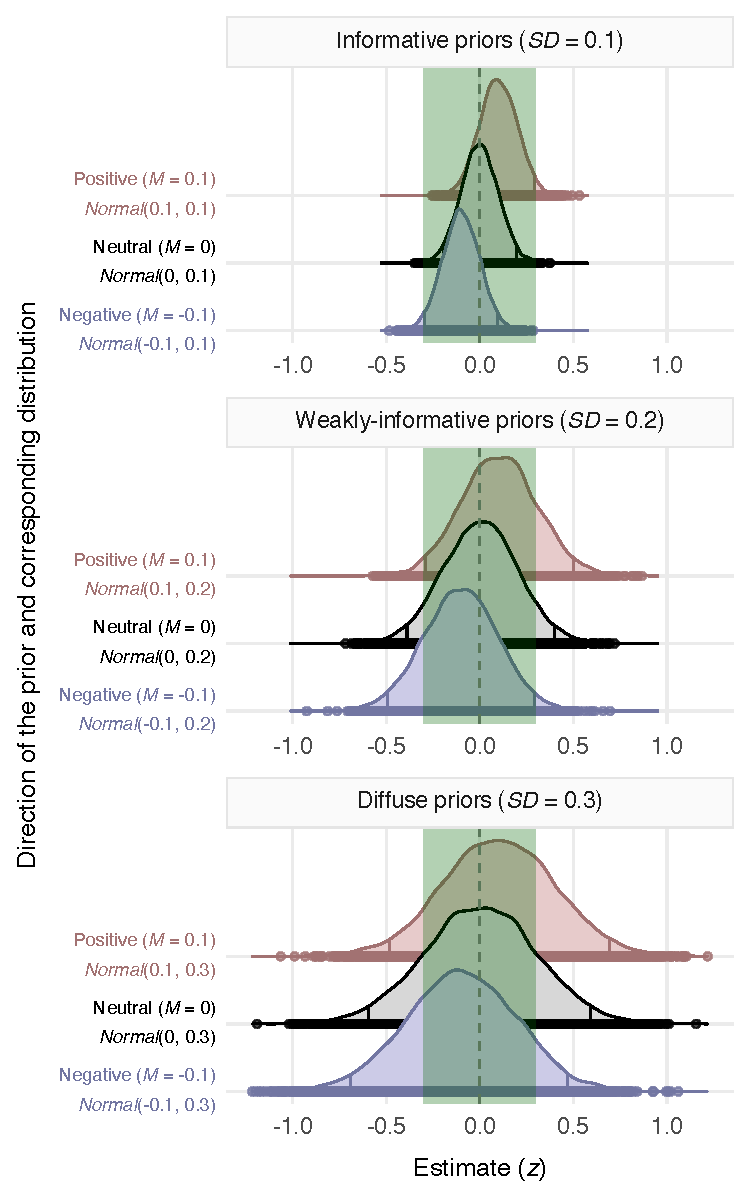
\includegraphics[width=1\linewidth]{/Users/pablodejuanbernabeu/Library/CloudStorage/OneDrive-LancasterUniversity/semanticpriming-semanticdecision-lexicaldecision/bayesian_priors/plots/bayesian_priors} 

}

\caption{Priors used in the three studies. The green vertical rectangle shows the range of plausible effect sizes based on relevant previous studies and on our frequentist analyses.}\label{fig:bayesian-priors}
\end{figure}

The adequacy of each of these priors was assessed with prior predictive checks, in which we compared the observed data to data predicted by the priors (Schoot et al., 2021). In these checks, we also tested the adequacy of two model-wide distributions: the traditional Gaussian distribution (default in most analyses) and an exponentially modified Gaussian---dubbed `ex-Gaussian'---distribution (Matzke \& Wagenmakers, 2009). The ex-Gaussian distribution was considered because the residual errors of the frequentist models were not normally distributed (Lo \& Andrews, 2015), and because this distribution was found to be more appropriate than the Gaussian one in a related, previous study (see supplementary materials of Rodríguez-Ferreiro et al., 2020). The ex-Gaussian distribution had an identity link function, which preserves the interpretability of the coefficients, as opposed to a transformation applied directly to the dependent variable (Lo \& Andrews, 2015).

Prior predictive checks revealed that the priors were adequate, and that the ex-Gaussian distribution was more appropriate than the Gaussian one, converging with Rodríguez-Ferreiro et al. (2020) (see the corresponding plots in \protect\hyperlink{appendix-D-interaction-plots}{\underline{Appendix D}}). Therefore, the ex-Gaussian distribution was used in the final models.

\hypertarget{prior-sensitivity-analysis}{%
\subparagraph{Prior sensitivity analysis}\label{prior-sensitivity-analysis}}

The priors were used in the main analyses within separate models. In other words, in each model, all priors had the same degree of informativeness (for similar approaches, see Pregla et al., 2021; Rodríguez-Ferreiro et al., 2020; Stone et al., 2021; Stone et al., 2020). In this way, a prior sensitivity analysis was performed to acknowledge the likely influence of the priors on the posterior distributions---that is, on the results (Lee \& Wagenmakers, 2014; Schoot et al., 2021; Stone et al., 2020).

\hypertarget{posterior-distributions}{%
\paragraph{Posterior distributions}\label{posterior-distributions}}

As a last diagnostic, posterior predictive checks were performed to assess the fit between the observed data and new data predicted by the posterior (Schoot et al., 2021). These checks are available in \protect\hyperlink{appendix-C-Bayesian-analysis-diagnostics}{\underline{Appendix C}}.

\hypertarget{general-method-for-statistical-power-analyses}{%
\subsection{General method for statistical power analyses}\label{general-method-for-statistical-power-analyses}}

Power curves based on Monte Carlo simulations were performed for most of the effects of interest, using the R package `simr', Version 1.0.5 (Green \& MacLeod, 2016). Obtaining power curves for a range of effects in each study allows for a comprehensive assessment of the plausibility of the power estimated for each effect.

Monte Carlo simulations are performed by running the statistical model a large number of times, under slight, random variations of the dependent variable (Green \& MacLeod, 2016; for a comparable approach, see Loken \& Gelman, 2017). The power to detect each effect of interest is calculated by dividing the number of times that the effect is significant by the total number of simulations run. For instance, if an effect is significant on 85 simulations out of 100, the power for that effect is 85\% (Kumle et al., 2021). The sample sizes tested in the semantic priming study ranged from 50 to 800 participants, whereas those tested in the semantic decision and lexical decision studies ranged from 50 to 2,000 participants. These sample sizes were unequally spaced to limit the computational requirements. They comprised the following: 50, 100, 200, 300, 400, 500, 600, 700, 800, 1,200, 1,600 and 2,000 participants.\footnote{For the semantic priming study, the remaining sample sizes up to 2,000 participants have not finished running yet. Upon finishing, they will be reported in this manuscript.} The variance of the results decreases as more simulations are run. In each of our three studies, 200 simulations (as in Brysbaert \& Stevens, 2018) were run for each effect of interest and for each sample size under consideration. Thus, for a power curve examining the power for an effect across 12 sample sizes, 2,400 simulations were run. In each study, the item-level sample size---i.e., the number of words---was not modified. Thus, each of the power curves we present assume the same number of words that existed in each of our studies (these numbers are detailed in each study below). \emph{P} values were calculated using the Satterthwaite approximation for degrees of freedom, which is faster than Kenward-Roger but similarly accurate (Luke, 2017).

It is difficult to determine an effect size for each effect examined in a power analysis, as the amount and the scope of relevant research are usually finite and biased (Albers \& Lakens, 2018; Gelman \& Carlin, 2014; Kumle et al., 2021). Power analyses sometimes use the original effect sizes from previous studies (e.g., Pacini \& Barnard, 2021; Villalonga et al., 2021). In contrast, some authors have opted to reduce the previous effect sizes to account for factors that can influence the effect size of the planned study. First, publication bias and low-powered studies cause published effect sizes to be inflated (Brysbaert, 2019; Loken \& Gelman, 2017; Open Science Collaboration, 2015; Vasishth et al., 2018; Vasishth \& Gelman, 2021). Second, there might be differences between the studies used in the power analysis and the study to be conducted. Some of these differences could be foreseeable---for instance, if they are due to a limitation in the literature available for the power analysis---, whereas other differences might arise from unexpected circumstances arising during the project or from random variation (Barsalou, 2019). Reducing the effect size in the power analysis leads to an increase of the sample size of the planned study (Brysbaert \& Stevens, 2018; Green \& MacLeod, 2016; Hoenig \& Heisey, 2001). The reduced effect size---sometimes dubbed the smallest effect size of interest---is often set with a certain arbitrariness. For instance, Fleur et al. (2020) applied a reduction of 1/8 (i.e., 12.5\%), whereas Kumle et al. (2021) applied a 15\% reduction. In the present study, a reduction of 20\% was applied to every effect examined in the power analysis. By comparison with the power analyses reviewed in this paragraph, the present reduction will lead to a relatively-conservative estimate of required sample sizes. Yet, it is intrinsically difficult to determine how conservative a power analysis is, once we consider the insufficient power of most studies in psychology, and the resulting overestimation of effect sizes.

Both the primary analysis and the power analysis were performed in R (R Core Team, 2021). Version 4.0.2 was used for the frequentist analysis, Version 4.1.0 was used for the Bayesian analysis, and Version 4.1.2 was used for fast operations such as plotting. All the statistical and the power analyses were run on the High-End Computing facility at Lancaster University.\footnote{Information about this facility is available at \url{https://answers.lancaster.ac.uk/display/ISS/High+End+Computing+\%28HEC\%29+help}}

\hypertarget{study-1-semantic-priming}{%
\section{Study 1: Semantic priming}\label{study-1-semantic-priming}}

The core data set in this study was that of the Semantic Priming Project (Hutchison et al., 2013; also see Yap et al., 2017). Out of the tasks delivered in the experiment, we used the lexical decision one because it was most relevant to our forthcoming research. In the lexical decision task, participants judged whether strings of letters constituted real words (e.g., `building') or nonwords (e.g., `gop'). Crucially, in the experimental manipulation that characterises semantic priming, a prime word was presented before the target word in each trial. Since prime words facilitate the comprehension of target words, the participants' responses to the targets can be analysed as a function of the semantic relationship between primes and targets (Hoedemaker \& Gordon, 2014).

In some studies, the association between prime and target words has been examined in terms of related versus unrelated pairs (Pecher et al., 1998; Trumpp et al., 2013), and in terms of first- and second-order relationships (Hutchison et al., 2013). In contrast to these categorical associations, other studies have measured the association between the prime and the target words using language-based similarity estimates (Günther et al., 2016a, 2016b; Hutchison et al., 2008; Jones et al., 2006; Lam et al., 2015; Lund et al., 1995; Lund \& Burgess, 1996; Mandera et al., 2017; McDonald \& Brew, 2002; Padó \& Lapata, 2007; Petilli et al., 2021; Wingfield \& Connell, 2022). In one of these studies, Mandera et al. (2017) found that the latter computational measures outperformed human-based associations at explaining the priming effect.

Priming associations beyond the linguistic realm have also been examined, with early studies finding perceptual priming effects (Flores d'Arcais et al., 1985; Schreuder et al., 1984). Yet, the earliest findings were soon reframed by Pecher et al. (1998), who conducted a follow-up with an improved design, and observed the perceptual priming effect only when the word processing task was preceded by a visually-intensive task (Pecher et al., 1998). This moderating condition, replicated by Yee et al. (2012), is consistent with other conceptual-processing studies using a non-priming paradigm (Ostarek \& Huettig, 2017). However, a considerable number of studies have observed perceptual priming even in the absence of a preparatory perceptual task. A set of these studies used the Conceptual Modality Switch paradigm, in which the primes and the targets are presented in separate, consecutive trials (Bernabeu et al., 2017; Collins et al., 2011; Hald et al., 2011, 2013; Louwerse \& Connell, 2011; Lynott \& Connell, 2009; Pecher et al., 2003; Trumpp et al., 2013). The other set of studies, using the more standard priming intervals, are described below.

Lam et al. (2015) conducted a semantic priming experiment containing a lexical decision task. Participants were instructed to respond whether the prime word and the target word in each trial were both real words or pseudowords. The semantic-priming manipulation consisted of the following types of associations between the prime and the target words: (1) semantic association (e.g., bolt → screwdriver), (2) action association (e.g., housekey → screwdriver), (3) visual association (e.g., soldering iron → screwdriver), and (4) no association (e.g., charger → screwdriver). In addition, four conditions were present that consisted of SOAs of 500, 650, 800 and 1,400 ms. In the results, Lam et al.~firstly observed priming effects of the semantic-association type with all SOAs. Secondly, the authors observed motor-association priming effects with the SOAs of 500, 650 and 1,400 ms. Lastly, they observed visual-association priming effects only with the SOA of 1,400 ms. Overall, semantic-association priming---corresponding to language-based association---was more consistent than the priming based on visual and action associations. This greater influence of the language system converges with other studies on semantic priming (Lam et al., 2015; Pecher et al., 1998; Petilli et al., 2021) and with studies using other paradigms (Banks et al., 2021; Kiela \& Bottou, 2014; Louwerse et al., 2015).

Similarly, the results of Lam et al. (2015) regarding the time course of language-based and vision-based priming were consistent with a wealth of literature observing that perceptual systems, such as vision, are activated later than the language system (Barsalou et al., 2008; Connell \& Lynott, 2013; Louwerse \& Connell, 2011; Santos et al., 2011). For instance, studies using electroencephalography have found that perceptual priming effects emerged in the first 300 ms. Following the 300-ms stage, the perceptual priming increased in some studies (Amsel et al., 2014; Bernabeu et al., 2017), whereas other studies it stabilised (Kiefer et al., 2022), and in a third set of studies, the effect fluctuated (Amsel, 2011). Taken together, the most prevalent pattern is of a gradual accumulation of information throughout word processing (also see Hauk, 2016), which is consistent with the accummulation of information required for the integration of context in sentences (Hald et al., 2006). This progression invites two hypotheses regarding SOA in the current study: (1) that language-based information will be more prevalent than vision-based information in both the short and the long SOA, and (2) that vision-based information will be more prevalent in the long SOA than in the short one. Consistent with the first hypothesis, Petilli et al. (2021) observed that language-based information was more influential in both the short and the long SOA, within the data set of Hutchison et al. (2013). The second hypothesis, in contrast, is challenged by other findings. First, Hutchison (2003) concluded that the vision-based priming effect was negligible. Second, other studies have observed the effect only when the word processing task was preceded by a visually-intensive task (Pecher et al., 1998; Yee et al., 2012). Third, Petilli et al.~observed vision-based priming with the short SOA (150 ms) but not with the long one (1,200 ms).

The findings of Petilli et al. (2021) were based on a novel analysis of the data set of Hutchison et al. (2013). The strengths of Petilli et al.'s study centred on the simultaneous analysis of language- and vision-based similarity using predictors that were continuous (see Cohen, 1983; Günther et al., 2016a; Mandera et al., 2017) and not based on human ratings (cf. Hutchison et al., 2008, 2013; Lam et al., 2015; Pecher et al., 1998). The authors used such measures to pursue a comprehensive analysis that was not affected by the problem of circularity between the independent and the dependent variables. The circularity problem obtains even though the participants who contributed to the ratings---or `norms'---are always different from those who participate in the main experiment.

Petilli et al.~operationalised language-based similarity based on text-based co-occurrence, producing a continuous measure in contrast to the categorical factors used earlier. Next, Petilli et al.~created a visual-similarity measure by retrieving ImageNet images for each word, and training vector representations on those images using neural networks. Importantly, the authors compared the resulting visual-similarity measure to previous scores based on human ratings (Pecher et al., 1998), and found a comparable pattern. Using these materials, Petilli et al.~examined language-based and vision-based priming in two tasks---lexical decision and naming---and with both a short and a long SOA. In lexical decision, the largest effect observed by the authors was that of language-based priming with the short SOA (150 ms). The second largest effect was that of language-based priming with the long SOA (1,200 ms). Next, the weakest effect that was significant was that of vision-based priming with the short SOA. Last, there was no effect of vision-based priming with the long SOA. Petilli et al. (2021) explained the absence of vision-based priming with the long SOA in lexical decision by contending that visual activation had likely decayed before participants processed the target words (also see Yee et al., 2011), owing to the limited semantic processing required for lexical decision (also see Balota \& Lorch, 1986; Becker et al., 1997; Connell \& Lynott, 2013; de Wit \& Kinoshita, 2015; Joordens \& Becker, 1997; Ostarek \& Huettig, 2017). Therefore, the authors suggested that perceptual simulation does \emph{not} outlast language-based processing in lexical decision, in contrast to the longer latency found in other tasks (Barsalou et al., 2008; Louwerse \& Connell, 2011).

In the naming task of Petilli et al. (2021), the largest effect was that of language-based priming with the long SOA. The second largest effect was that of language-based priming with the short SOA. Last, there was no effect of vision-based priming with either SOA. This finding contrasted with Connell and Lynott (2014), who found facilitatory effects of visual strength in both lexical decision and naming. Petilli et al.~explained the lack of vision-based priming in the naming task by alluding to the lower semantic depth of this task---compared to lexical decision---, and the mixture of visual and auditory processing in the naming task (Connell \& Lynott, 2014).

In the present study, we revisited the interplay between linguistic and perceptual simulation by conceptually replicating Petilli et al. (2021). Specifically, we used the same primary data set (Hutchison et al., 2013), and a language-based similarity measure that was very similar to that used by Petilli et al. (2021; both our measure and theirs originated from Mandera et al., 2017). In contrast, in the domain of vision, the operationalisation of visual-strength difference in our study---based one variable from (Lynott et al., 2020)---was simpler than that of Petilli et al.'s visual similarity---which involved convolutional neural networks. As a counterpoint, Petilli et al.'s measure was superior in that it was independent from human ratings, thus precluding the problem of circularity between the independent and the dependent variables. At \protect\hyperlink{comparing-two-measures-of-vision-based-information}{\underline{the end of the Results section}}, we compare the performance of these two measures.

\hypertarget{methods-1}{%
\subsection{Methods}\label{methods-1}}

\hypertarget{effects-of-interest}{%
\subsubsection{Effects of interest}\label{effects-of-interest}}

\begin{itemize}
\item
  Z-scored vocabulary size {[}\texttt{z\_vocabulary\_size}; calculated from average of \texttt{vocaba}, \texttt{vocabb} and \texttt{vocabc} in Hutchison et al. (2013){]}. The test used by Hutchison et al. (2013) comprised a synonym test, an antonym test, and an analogy test, all three extracted from the Woodcock--Johnson III diagnostic reading battery (Woodcock et al., 2001). We operationalised the vocabulary measure as the mean score across the three tasks per participant.
\item
  Z-scored, recoded participant's gender {[}\texttt{z\_recoded\_participant\_gender}; calculated from \texttt{gender} in Hutchison et al. (2013){]}
\item
  Z-scored language-based similarity between prime and target words {[}\texttt{z\_cosine\_similarity}{]}. This measure was calculated using a semantic space from Mandera et al. (2017), which the authors found to be the second-best predictor (\(R\)\textsuperscript{2} = .465) of the semantic priming effect in the lexical decision task of Hutchison et al. (2013) (we could not use the best semantic space, \(R\)\textsuperscript{2} = .471, owing to computational limitations). The second-best semantic space (see first row in Table 5 of Mandera et al., 2017) was based on lemmas from a subtitle corpus, processed in a Continuous Bag Of Words model, and the space had 300 dimensions and a window size of 6.
\item
  Z-scored vision-based information in words {[}\texttt{z\_visual\_rating}; calculated from \texttt{Visual.mean} in Lynott et al. (2020){]}
\item
  Z-scored, recoded SOA {[}\texttt{z\_recoded\_interstimulus\_interval}; calculated from \texttt{isi} in Hutchison et al. (2013){]}
\end{itemize}

The final data set contained 496 participants, 5,943 prime-target pairs, and a total of 345,666 RTs. On average, there were 697 prime-target pairs per participant (\(SD\) = 33.34), and conversely, 58 participants per prime-target pair (\(SD\) = 4.25).

Figure \ref{fig:semanticpriming-correlations} shows the zero-order correlations among the predictors and the dependent variable.

\begin{figure}

{\centering 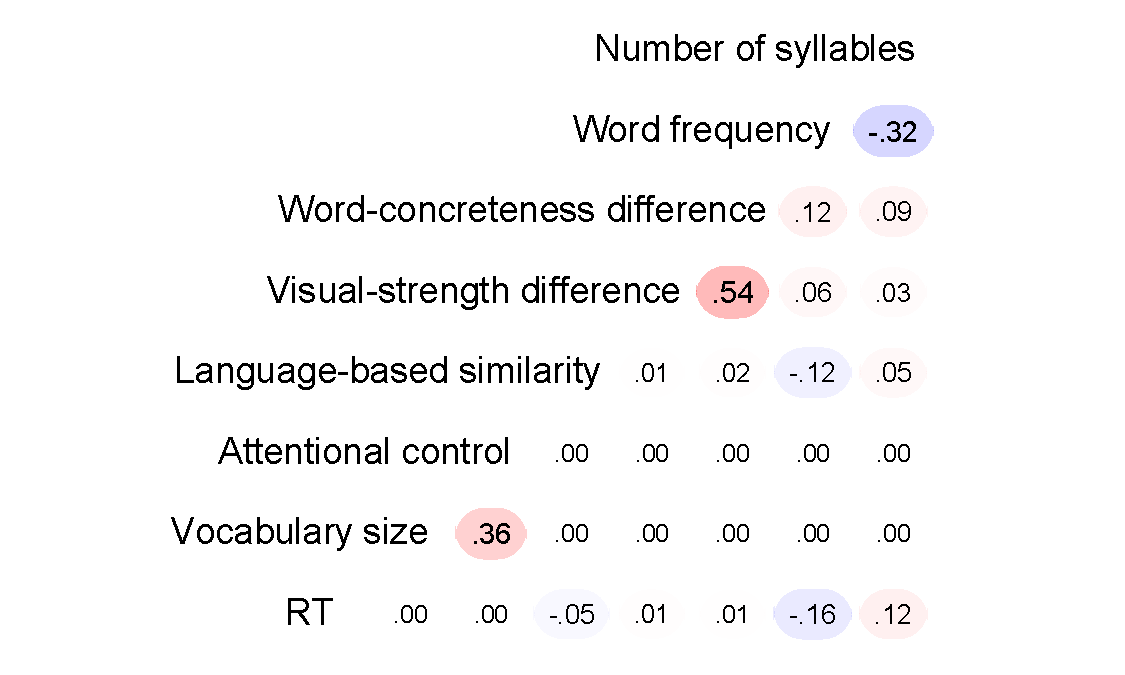
\includegraphics[width=0.65\linewidth]{manuscript_files/figure-latex/semanticpriming-correlations-1} 

}

\caption{Zero-order correlations in the semantic priming study.}\label{fig:semanticpriming-correlations}
\end{figure}

\hypertarget{covariates}{%
\subsubsection{Covariates}\label{covariates}}

The following covariates were included in the model to allow a rigorous analysis of the effects of interest.

\begin{itemize}
\item
  Lexical (see \protect\hyperlink{appendix-A-lexical-covariates}{\underline{Appendix A}}): z-scored word frequency and orthographic Levenshtein distance (Balota et al., 2007)
\item
  Semantic: z-scored word concreteness (Brysbaert et al., 2014), used as a covariate of visual rating.
\item
  Individual differences: z-scored attentional control (Hutchison et al., 2013). This covariate is related to vocabulary size (Ratcliff et al., 2010), and previous studies have pointed out the desirability of including these kinds of covariates in analyses (James et al., 2018; Pexman \& Yap, 2018). Attentional control was operationalised as the average score across three attention-demanding tasks: namely, operation span, Stroop, antisaccade.
\end{itemize}

\hypertarget{diagnostics-for-the-frequentist-model}{%
\subsubsection{Diagnostics for the frequentist model}\label{diagnostics-for-the-frequentist-model}}

The model presented convergence warnings. To avoid removing important random slopes, which could increase the Type I error (Brauer \& Curtin, 2018; Singmann \& Kellen, 2019), we examined the model after refitting it using seven optimization algorithms through the `allFit' function of the `lme4' package (Bates et al., 2021). The results showed that all optimizers produced virtually identical means for all effects, suggesting that the convergence warnings were not consequential (Bates et al., 2021) (see \protect\hyperlink{appendix-B-frequentist-analysis-diagnostics}{\underline{Appendix B}}).

The residual errors were not normally distributed, and attempts to mitigate this deviation proved unsuccessful (see \protect\hyperlink{appendix-B-frequentist-analysis-diagnostics}{\underline{Appendix B}}). However, this is not likely to have posed a major problem, as mixed-effects models are fairly robust to deviations from normality (Knief \& Forstmeier, 2021; Schielzeth et al., 2020).

The model did not present multicollinearity problems, all variance inflation factors (VIF) being smaller than 2 (Dormann et al., 2013; Harrison et al., 2018).

\hypertarget{diagnostics-for-the-bayesian-model}{%
\subsubsection{Diagnostics for the Bayesian model}\label{diagnostics-for-the-bayesian-model}}

Three Bayesian models were run that were respectively characterised by informative, weakly-informative and diffuse priors. In each model, 16 chains were used. In each chain, 1,500 warmup iterations were run, followed by 4,500 post-warmup iterations. Thus, a total of 72,000 post-warmup draws were produced over all the chains.

The maximum \(\widehat R\) value for the fixed effects across the three models was 1.00, suggesting that these parameters had converged (Schoot et al., 2021; Vehtari et al., 2021). In contrast, the maximum \(\widehat R\) value for the random effects was 1.13, exceeding the 1.01 threshold (Vehtari et al., 2021). Therefore, models with more iterations will be run, and once completed, they will be reported in this manuscript.

The posterior predictive checks were sound (see \protect\hyperlink{appendix-C-Bayesian-analysis-diagnostics}{\underline{Appendix C}}). Furthermore, in the prior sensitivity analysis, the results were virtually identical with the three priors that were considered (to recall the priors, see Figure \ref{fig:bayesian-priors} above; to view the results in detail, see \protect\hyperlink{appendix-E-Bayesian-analysis-results}{\underline{Appendix E}}).

\hypertarget{semanticpriming-results}{%
\subsection{Results}\label{semanticpriming-results}}

Table \ref{tab:semanticpriming-frequentist-model} presents the results of the mixed-effects model.

\begin{table}[!h]

\caption{\label{tab:semanticpriming-frequentist-model}Frequentist model for the semantic priming study.}
\centering
\begin{threeparttable}
\begin{tabular}[t]{lrrrrr}
\toprule
\multicolumn{1}{c}{ } & \multicolumn{1}{c}{$\upbeta$} & \multicolumn{1}{c}{$SE$} & \multicolumn{1}{c}{95\% CI} & \multicolumn{1}{c}{$t$} & \multicolumn{1}{c}{$p$}\\
\midrule
(Intercept) & 0.00 & 0.00 & {}[0.00, 0.01] & 1.59 & .112\\
\addlinespace[0.3em]
\multicolumn{6}{l}{\textbf{Individual differences}}\\
\cellcolor{gray!6}{\hspace{1em}Attentional control} & \cellcolor{gray!6}{0.00} & \cellcolor{gray!6}{0.00} & \cellcolor{gray!6}{{}[0.00, 0.00]} & \cellcolor{gray!6}{-0.56} & \cellcolor{gray!6}{.577}\\
\hspace{1em}Vocabulary size $^{\text{a}}$ & 0.00 & 0.00 & {}[0.00, 0.00] & 0.02 & .987\\
\hspace{1em}Gender $^{\text{a}}$ & 0.00 & 0.00 & {}[0.00, 0.00] & -0.03 & .979\\
\addlinespace[0.3em]
\multicolumn{6}{l}{\textbf{Target-word lexical covariates}}\\
\cellcolor{gray!6}{\hspace{1em}Word frequency} & \cellcolor{gray!6}{-0.16} & \cellcolor{gray!6}{0.00} & \cellcolor{gray!6}{{}[-0.16, -0.15]} & \cellcolor{gray!6}{-49.40} & \cellcolor{gray!6}{<.001}\\
\cellcolor{gray!6}{\hspace{1em}Number of syllables} & \cellcolor{gray!6}{0.07} & \cellcolor{gray!6}{0.00} & \cellcolor{gray!6}{{}[0.07, 0.08]} & \cellcolor{gray!6}{22.81} & \cellcolor{gray!6}{<.001}\\
\addlinespace[0.3em]
\multicolumn{6}{l}{\textbf{Prime-target semantic relationship}}\\
\cellcolor{gray!6}{\hspace{1em}Word-concreteness difference} & \cellcolor{gray!6}{0.01} & \cellcolor{gray!6}{0.00} & \cellcolor{gray!6}{{}[0.01, 0.02]} & \cellcolor{gray!6}{3.48} & \cellcolor{gray!6}{.001}\\
\hspace{1em}Language-based similarity $^{\text{b}}$ & -0.08 & 0.00 & {}[-0.08, -0.07] & -22.44 & <.001\\
\hspace{1em}Visual-strength difference $^{\text{b}}$ & 0.01 & 0.00 & {}[0.01, 0.02] & 4.18 & <.001\\
\addlinespace[0.3em]
\multicolumn{6}{l}{\textbf{Task condition}}\\
\hspace{1em}Stimulus-onset asynchrony (SOA) $^{\text{b}}$ & 0.06 & 0.01 & {}[0.04, 0.07] & 7.47 & <.001\\
\addlinespace[0.3em]
\multicolumn{6}{l}{\textbf{Interactions}}\\
\cellcolor{gray!6}{\hspace{1em}\makecell[l]{Word-concreteness difference  $\times$ \\ \hspace{0.3cm} Vocabulary size}} & \cellcolor{gray!6}{0.00} & \cellcolor{gray!6}{0.00} & \cellcolor{gray!6}{{}[0.00, 0.01]} & \cellcolor{gray!6}{1.31} & \cellcolor{gray!6}{.189}\\
\cellcolor{gray!6}{\hspace{1em}Word-concreteness difference  $\times$  SOA} & \cellcolor{gray!6}{0.00} & \cellcolor{gray!6}{0.00} & \cellcolor{gray!6}{{}[0.00, 0.01]} & \cellcolor{gray!6}{2.57} & \cellcolor{gray!6}{.010}\\
\cellcolor{gray!6}{\hspace{1em}Word-concreteness difference  $\times$  Gender} & \cellcolor{gray!6}{0.00} & \cellcolor{gray!6}{0.00} & \cellcolor{gray!6}{{}[-0.01, 0.00]} & \cellcolor{gray!6}{-0.97} & \cellcolor{gray!6}{.332}\\
\cellcolor{gray!6}{\hspace{1em}\makecell[l]{Language-based similarity  $\times$ \\ \hspace{0.3cm} Attentional control}} & \cellcolor{gray!6}{-0.01} & \cellcolor{gray!6}{0.00} & \cellcolor{gray!6}{{}[-0.01, 0.00]} & \cellcolor{gray!6}{-2.46} & \cellcolor{gray!6}{.014}\\
\cellcolor{gray!6}{\hspace{1em}\makecell[l]{Visual-strength difference  $\times$ \\ \hspace{0.3cm} Attentional control}} & \cellcolor{gray!6}{0.00} & \cellcolor{gray!6}{0.00} & \cellcolor{gray!6}{{}[0.00, 0.00]} & \cellcolor{gray!6}{0.24} & \cellcolor{gray!6}{.810}\\
\hspace{1em}\makecell[l]{Language-based similarity  $\times$ \\ \hspace{0.3cm} Vocabulary size} & -0.01 & 0.00 & {}[-0.01, 0.00] & -2.34 & .020\\
\hspace{1em}\makecell[l]{Visual-strength difference  $\times$ \\ \hspace{0.3cm} Vocabulary size} & 0.00 & 0.00 & {}[-0.01, 0.00] & -1.37 & .172\\
\hspace{1em}Language-based similarity  $\times$  Gender & 0.00 & 0.00 & {}[-0.01, 0.00] & -0.79 & .433\\
\hspace{1em}Visual-strength difference  $\times$  Gender & 0.00 & 0.00 & {}[0.00, 0.01] & 1.46 & .144\\
\hspace{1em}Language-based similarity  $\times$  SOA $^{\text{b}}$ & 0.01 & 0.00 & {}[0.00, 0.01] & 3.22 & .001\\
\hspace{1em}Visual-strength difference  $\times$  SOA $^{\text{b}}$ & 0.00 & 0.00 & {}[-0.01, 0.00] & -2.25 & .025\\
\bottomrule
\end{tabular}
\begin{tablenotes}
\item \textit{\linebreak} 
\item \textit{Note}. $\upbeta$ = Estimate based on z-scored variables; \textit{SE} = standard error; \linebreak \phantom{.}CI = confidence interval. Shaded rows contain covariates. Some interactions are \linebreak \phantom{.}split over two lines, with the second line indented. \linebreak \linebreak \phantom{.}$^{\text{a}}$ By-word random slopes were included for this effect. \linebreak \phantom{.}$^{\text{b}}$ By-participant random slopes were included for this effect.
\end{tablenotes}
\end{threeparttable}
\end{table}

The fixed effects of this model explained 4.22\% of the variance, and the random effects explained 11.01\% (Nakagawa et al., 2017). It is to be expected that random effects explain more variance, as they involve a far larger number of coefficients for each effect. For instance, the by-word random slopes for a single individual-level variable (e.g., vocabulary size) involve as many coefficients as the number of words. Similarly, the by-participant random slopes for a single word-level variable (e.g., language-based similarity) involve as many coefficients as the number of participants. In contrast, a fixed effect involves 1 coefficient only.

Figure \ref{fig:semanticpriming-interactions-with-vocabulary-size}-a shows the interaction between vocabulary size and language-based similarity, whereby higher-vocabulary participants presented a greater benefit from the language-based similarity between prime and target words. That is, the greater the similarity between prime and target words, the greater the advantage for participants with higher vocabularies. This interaction replicates the results of Yap et al. (2017), who analysed the same data set but using a categorical measure of similarity instead. Indeed, this replication is noteworthy as it holds in spite of some methodological differences between the studies. First, Yap et al. (2017) operationalised the priming effect as a categorical difference between related and unrelated prime-target pairs. In contrast, the present study applied a continuous measure of relatedness---i.e., cosine similarity---, which is more precise and may thus afford more statistical power (Mandera et al., 2017; Petilli et al., 2021). Second, the analysis conducted by Yap et al. (2017) was correlational, whereas the present analysis used mixed-effects models that included several covariates to measure the effects of interest as rigorously as possible.

Figure \ref{fig:semanticpriming-interactions-with-vocabulary-size}-b presents the interaction between vocabulary size and vision-based similarity. Albeit a non-significant interaction, it is noteworthy that the effect of vision-based information is larger in lower-vocabulary participants.



\begin{figure}

{\centering 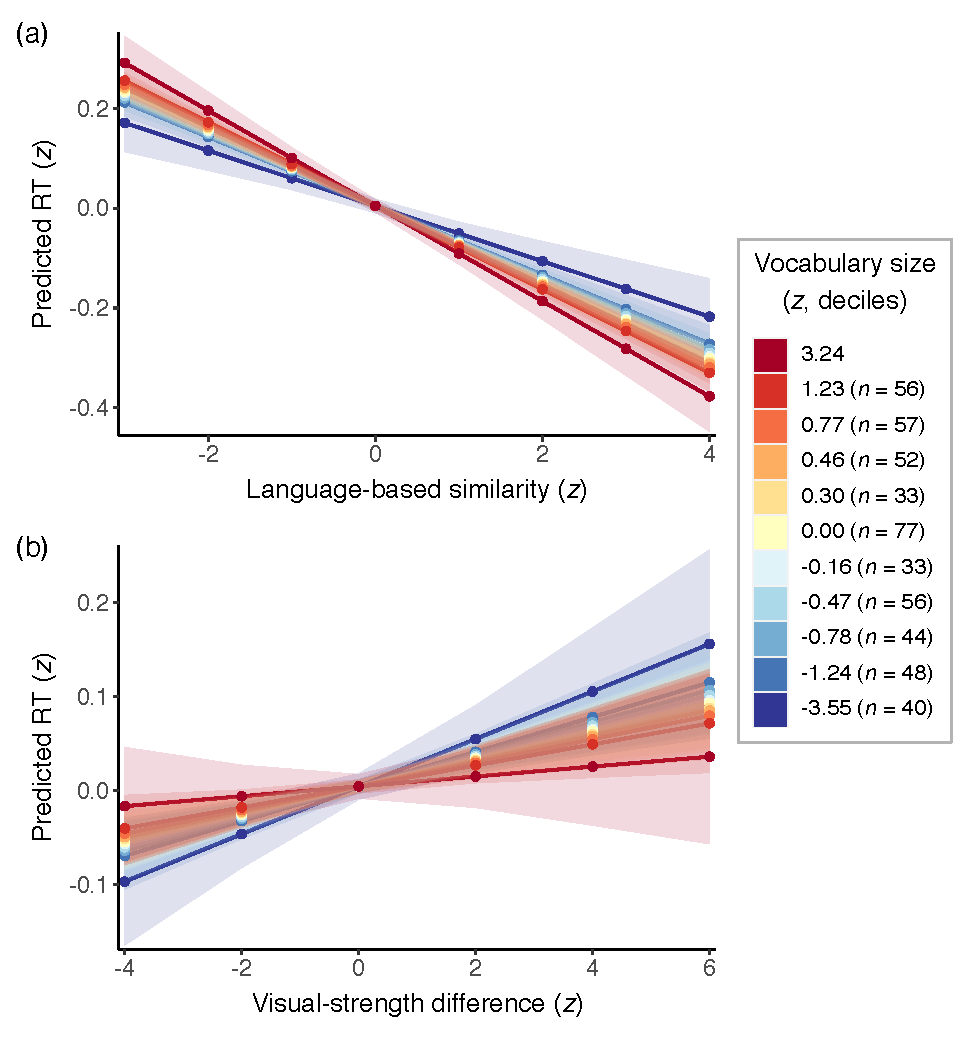
\includegraphics[width=0.85\linewidth]{/Users/pablodejuanbernabeu/Library/CloudStorage/OneDrive-LancasterUniversity/semanticpriming-semanticdecision-lexicaldecision/semanticpriming/frequentist_analysis/plots/semanticpriming-interactions-with-vocabulary-size} 

}

\caption{Interactions of vocabulary size with language- and vision-based similarity. Vocabulary size is constrained to deciles, whereas in the statistical analysis it contained more values within the current range. \emph{n} = number of participants contained between decile values.}\label{fig:semanticpriming-interactions-with-vocabulary-size}
\end{figure}

Methodologically, the interaction between vocabulary size and language-based similarity underscores the consistency that exists between human ratings and computational approximations to meaning (e.g., Charbonnier \& Wartena, 2019, 2020; Günther et al., 2016b; Louwerse et al., 2015; Mandera et al., 2017; Petilli et al., 2021; Solovyev, 2021; Wingfield \& Connell, 2022). In contrast to this consistency, some studies have found human ratings to have more explanatory power than computational measures (De Deyne et al., 2016, 2019; Gagné et al., 2016; Schmidtke et al., 2018), and other research has suggested that some computational measures are not intrinsically contentful, but arise from a missing-data problem (Snefjella \& Blank, 2020). In sum, this evidence suggests that computational measures are artificial, and yet valid for the study of cognition.

Figure \ref{fig:semanticpriming-interactions-with-SOA} shows that the effects of language-based similarity and visual strength were both larger with the short SOA. Yet there is a notable difference: whereas the effect of language-based similarity is present with both SOAs (i.e., 150 ms and 1,200 ms), the effect of visual strength is almost reserved to the the long SOA. This finding replicates Petilli et al. (2021), and stands in contrast to previous findings regarding the slower pace of the visual system in semantic priming (Lam et al., 2015) and in other paradigms (Connell \& Lynott, 2013; Louwerse \& Connell, 2011). \textbf{conclude}\_\_\_\_\_\_\_\_\_\_\_\_\_

\begin{figure}

{\centering 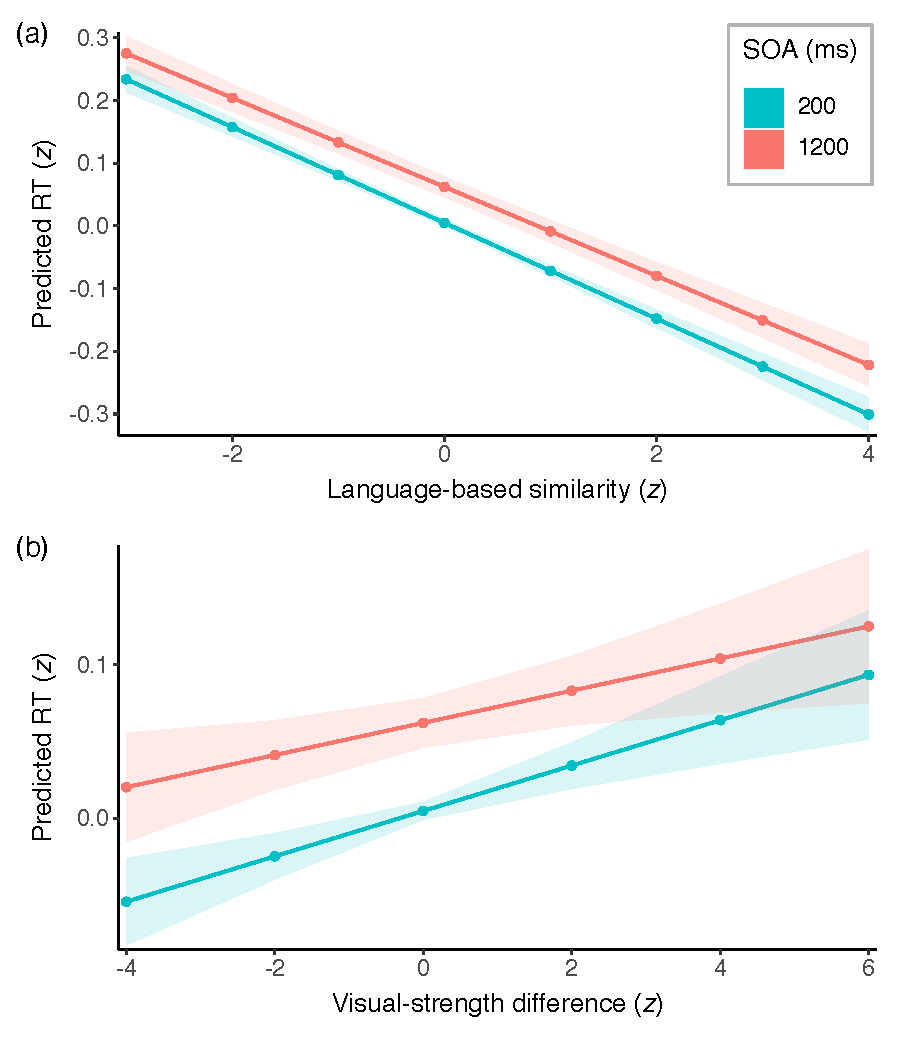
\includegraphics[width=0.8\linewidth]{/Users/pablodejuanbernabeu/Library/CloudStorage/OneDrive-LancasterUniversity/semanticpriming-semanticdecision-lexicaldecision/semanticpriming/frequentist_analysis/plots/semanticpriming-interactions-with-SOA} 

}

\caption{Interactions of SOA with language-based similarity and visual strength. SOA was analysed using z-scores, but for clarity, the variable is shown in its simpler form here.}\label{fig:semanticpriming-interactions-with-SOA}
\end{figure}

\hypertarget{the-importance-of-outliers}{%
\paragraph{The importance of outliers}\label{the-importance-of-outliers}}

The interaction in Figure \ref{fig:semanticpriming-interactions-with-vocabulary-size} is patent in all deciles of vocabulary size but most notably in the participants who lie more than 1 standard deviation away from the mean. Outliers in individual differences have played important roles in other areas of cognition as well, such as in the domains of aphantasia and hyperphantasia---traits characterised, respectively, by a diminished and an extraordinary ability to mentally visualise objects (Milton et al., 2021; Zeman et al., 2020). Furthermore, if we consider the difficulty of detecting effects involving individual differences (Diaz et al., 2021; Hedge et al., 2018; Rodríguez-Ferreiro et al., 2020), and the limited representativeness of most participant samples (Henrich et al., 2010), it seems recommendable to examine more varied samples in future studies, where possible.

\hypertarget{visualising-the-estimates}{%
\subsubsection{Visualising the estimates}\label{visualising-the-estimates}}

Figure \ref{fig:semanticpriming-frequentist-bayesian-plot-informativepriors-exgaussian} presents the posterior distribution of each effect, based on the informative prior model (for the models with the other priors, see \protect\hyperlink{appendix-E-Bayesian-analysis-results}{\underline{Appendix E}}). The frequentist estimates are also shown to facilitate the comparison with them.

\begin{figure}

{\centering 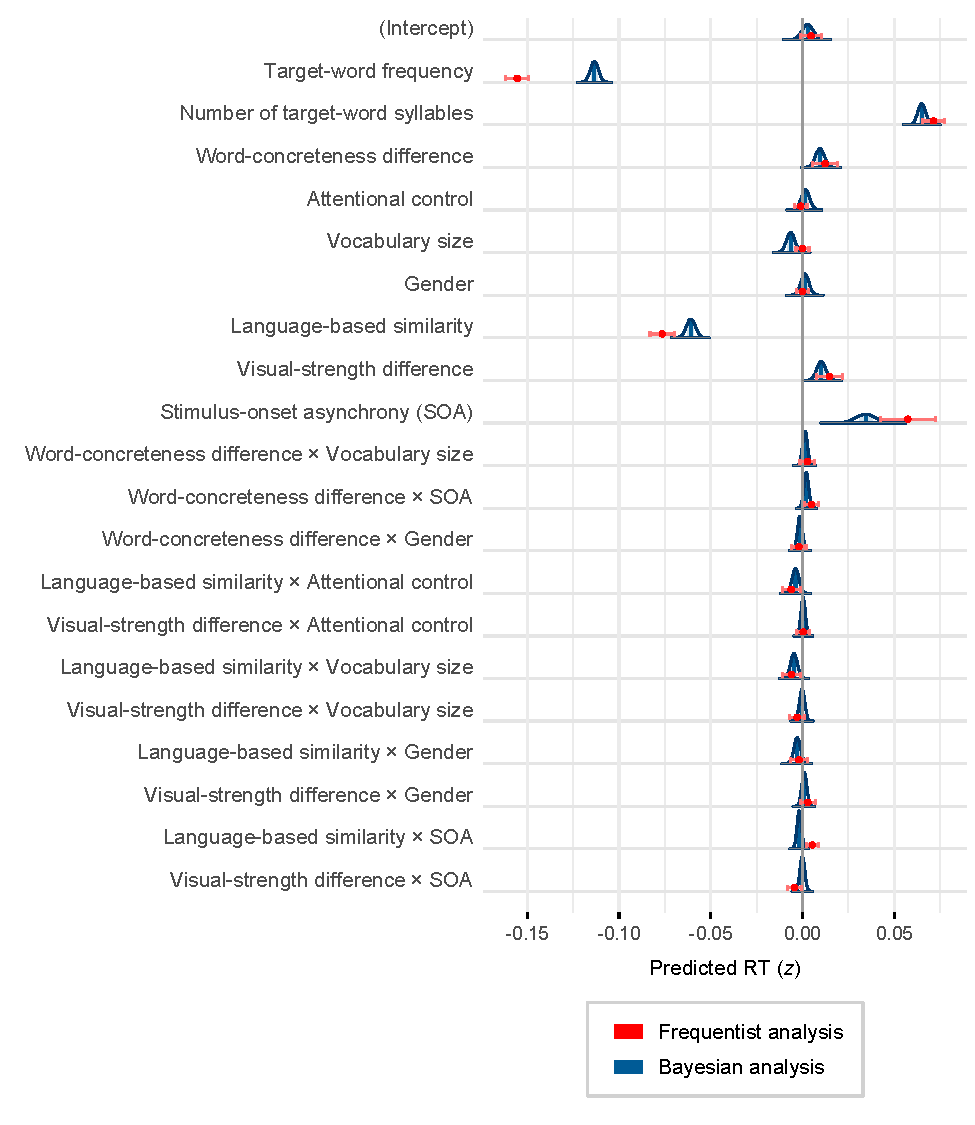
\includegraphics[width=1\linewidth]{/Users/pablodejuanbernabeu/Library/CloudStorage/OneDrive-LancasterUniversity/semanticpriming-semanticdecision-lexicaldecision/semanticpriming/frequentist_bayesian_plots/plots/semanticpriming_frequentist_bayesian_plot_informativepriors_exgaussian} 

}

\caption{Estimates from the frequentist analysis (in red) and from the Bayesian analysis (in blue) for the semantic priming study. The frequentist means (represented by points) are flanked by 95\% confidence intervals. The Bayesian means (represented by vertical lines) are flanked by 95\% credible intervals, in light blue (in some cases, the interval is covered up by the bar of the mean).}\label{fig:semanticpriming-frequentist-bayesian-plot-informativepriors-exgaussian}
\end{figure}

\hypertarget{comparing-two-measures-of-vision-based-information}{%
\subsubsection{Comparing two measures of vision-based information}\label{comparing-two-measures-of-vision-based-information}}

Next, we reflected on the adequacy of visual-strength difference as a measurement instrument, as it had never been used before to operationalise the semantic priming effect. On the one hand, its effect on RT was negative, as we would expect. However, we were concerned about the low correlation between this variable and language-based similarity (\(r\) = 0.01). This concern was especially motivated by the correlation that Petilli et al. (2021) had found between their `vision-based similarity' measure and language-based similarity, which reached \(r\) = .50. Based on this information, we set out to run a model with the aim of comparing the performance of our measures of vision-based information.

We created a subset of our data set in which we ensured that all the trials contained data from all the relevant variables---i.e., from all the existing variables and from the newly-added visual similarity from Petilli et al.~This subsetting resulted in the loss of 83\% of trials, owing to the strict selection criteria applied by Petilli et al.~in the creation of the visual-similarity measure (e.g., both the target and the prime word had to be associated to at least 100 pictures in ImageNet). As a result, our data set in this analysis contained 496 participants, 1,091 prime-target pairs, and a total of 254,140 RTs. On average, there were 128 prime-target pairs per participant (\(SD\) = 10.37), and conversely, 58 participants per prime-target pair (\(SD\) = 4.90).

Figure \ref{fig:semanticpriming-with-visualsimilarity-correlations} shows the zero-order correlations among the predictors and the dependent variable.

\begin{figure}

{\centering 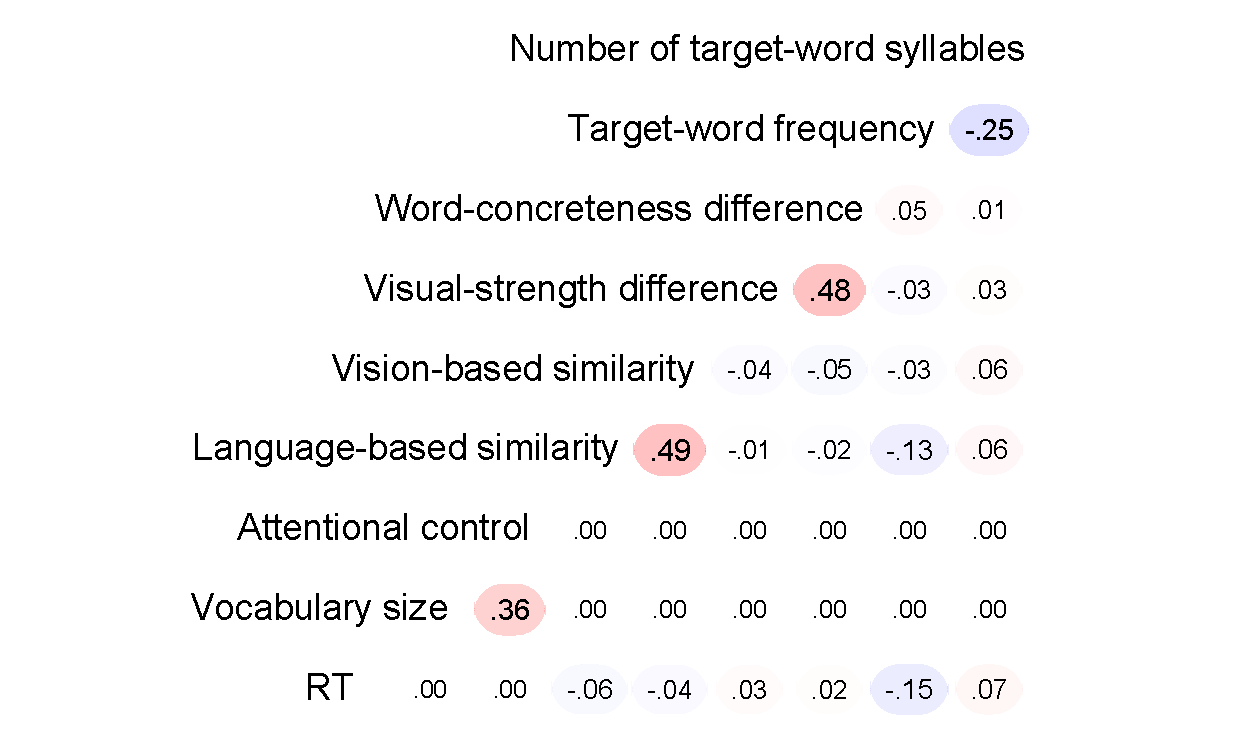
\includegraphics[width=0.73\linewidth]{manuscript_files/figure-latex/semanticpriming-with-visualsimilarity-correlations-1} 

}

\caption{Zero-order correlations in the semantic priming data set that included visual similarity.}\label{fig:semanticpriming-with-visualsimilarity-correlations}
\end{figure}

\hypertarget{diagnostics-for-the-frequentist-model-1}{%
\subsubsection{Diagnostics for the frequentist model}\label{diagnostics-for-the-frequentist-model-1}}

The model presented convergence warnings. To avoid removing important random slopes, which could increase the Type I error (Brauer \& Curtin, 2018; Singmann \& Kellen, 2019), we examined the model after refitting it using seven optimization algorithms through the `allFit' function of the `lme4' package (Bates et al., 2021). The results showed that all optimizers produced virtually identical means for all effects, suggesting that the convergence warnings were not consequential {[}Bates et al. (2021); see \protect\hyperlink{appendix-B-frequentist-analysis-diagnostics}{\underline{Appendix B}}{]}.

The residual errors were not normally distributed, and attempts to mitigate this deviation proved unsuccessful (see \protect\hyperlink{appendix-B-frequentist-analysis-diagnostics}{\underline{Appendix B}}). However, this is not likely to have posed a major problem, as mixed-effects models are fairly robust to deviations from normality (Knief \& Forstmeier, 2021; Schielzeth et al., 2020).

The model did not present multicollinearity problems, all VIFs being smaller than 2 (Dormann et al., 2013; Harrison et al., 2018).

Due to time constraints, this analysis did not include a Bayesian model.

\hypertarget{results}{%
\paragraph{Results}\label{results}}

Table \ref{tab:semanticpriming-with-visualsimilarity-frequentist-model} presents the results of the mixed-effects model. Due to space, the covariates are shown in Table \ref{tab:semanticpriming-with-visualsimilarity-frequentist-model-covariates}.

\begin{table}[!h]

\caption{\label{tab:semanticpriming-with-visualsimilarity-frequentist-model}Effects of interest in the semantic priming model that included visual similarity.}
\centering
\begin{threeparttable}
\begin{tabular}[t]{lrrrrr}
\toprule
\multicolumn{1}{c}{ } & \multicolumn{1}{c}{$\upbeta$} & \multicolumn{1}{c}{$SE$} & \multicolumn{1}{c}{95\% CI} & \multicolumn{1}{c}{$t$} & \multicolumn{1}{c}{$p$}\\
\midrule
(Intercept) & 0.01 & 0.01 & {}[-0.01, 0.02] & 0.90 & .370\\
\addlinespace[0.3em]
\multicolumn{6}{l}{\textbf{Individual differences}}\\
\hspace{1em}Vocabulary size $^{\text{a}}$ & 0.00 & 0.00 & {}[-0.01, 0.01] & 0.21 & .834\\
\hspace{1em}Gender $^{\text{a}}$ & 0.00 & 0.00 & {}[-0.01, 0.01] & -0.05 & .962\\
\addlinespace[0.3em]
\multicolumn{6}{l}{\textbf{Prime-target semantic relationship}}\\
\hspace{1em}Language-based similarity $^{\text{b}}$ & -0.07 & 0.01 & {}[-0.09, -0.06] & -8.33 & <.001\\
\hspace{1em}Visual-strength difference $^{\text{b}}$ & 0.03 & 0.01 & {}[0.01, 0.04] & 3.04 & .002\\
\hspace{1em}Vision-based similarity $^{\text{b}}$ & -0.02 & 0.01 & {}[-0.04, -0.01] & -2.55 & .011\\
\addlinespace[0.3em]
\multicolumn{6}{l}{\textbf{Task condition}}\\
\hspace{1em}Stimulus-onset asynchrony (SOA) $^{\text{b}}$ & 0.06 & 0.01 & {}[0.04, 0.08] & 6.80 & <.001\\
\addlinespace[0.3em]
\multicolumn{6}{l}{\textbf{Interactions}}\\
\hspace{1em}\makecell[l]{Language-based similarity  $\times$ \\ \hspace{0.3cm} Vocabulary size} & -0.01 & 0.01 & {}[-0.02, 0.01] & -0.96 & .339\\
\hspace{1em}\makecell[l]{Visual-strength difference  $\times$ \\ \hspace{0.3cm} Vocabulary size} & -0.01 & 0.01 & {}[-0.02, 0.01] & -1.02 & .309\\
\hspace{1em}\makecell[l]{Vision-based similarity  $\times$ \\ \hspace{0.3cm} Vocabulary size} & 0.00 & 0.01 & {}[-0.01, 0.01] & -0.01 & .991\\
\hspace{1em}Language-based similarity  $\times$  Gender & 0.00 & 0.01 & {}[-0.02, 0.01] & -0.75 & .456\\
\hspace{1em}Visual-strength difference  $\times$  Gender & -0.01 & 0.01 & {}[-0.02, 0.01] & -1.05 & .294\\
\hspace{1em}Vision-based similarity  $\times$  Gender & 0.00 & 0.01 & {}[-0.01, 0.01] & 0.39 & .696\\
\hspace{1em}Language-based similarity  $\times$  SOA $^{\text{b}}$ & 0.00 & 0.00 & {}[0.00, 0.01] & 0.87 & .382\\
\hspace{1em}Visual-strength difference  $\times$  SOA $^{\text{b}}$ & -0.01 & 0.00 & {}[-0.02, 0.00] & -2.60 & .010\\
\hspace{1em}Vision-based similarity  $\times$  SOA $^{\text{b}}$ & 0.01 & 0.00 & {}[0.00, 0.01] & 1.28 & .201\\
\bottomrule
\end{tabular}
\begin{tablenotes}
\item \textit{\linebreak} 
\item \textit{Note}. $\upbeta$ = Estimate based on z-scored variables; \textit{SE} = standard error; \linebreak \phantom{.}CI = confidence interval. Covariates shown in next table due to space. Some  \linebreak \phantom{.}interactions are split over two lines, with the second line indented. \linebreak \linebreak \phantom{.}$^{\text{a}}$ By-word random slopes were included for this effect. \linebreak \phantom{.}$^{\text{b}}$ By-participant random slopes were included for this effect.
\end{tablenotes}
\end{threeparttable}
\end{table}

\begin{table}[!h]

\caption{\label{tab:semanticpriming-with-visualsimilarity-frequentist-model-covariates}Covariates in the semantic priming model that included visual similarity.}
\centering
\begin{threeparttable}
\begin{tabular}[t]{lrrrrr}
\toprule
\multicolumn{1}{c}{ } & \multicolumn{1}{c}{$\upbeta$} & \multicolumn{1}{c}{$SE$} & \multicolumn{1}{c}{95\% CI} & \multicolumn{1}{c}{$t$} & \multicolumn{1}{c}{$p$}\\
\midrule
\addlinespace[0.3em]
\multicolumn{6}{l}{\textbf{Individual-differences covariate}}\\
\hspace{1em}Attentional control & 0.00 & 0.00 & {}[-0.01, 0.00] & -1.06 & .288\\
\addlinespace[0.3em]
\multicolumn{6}{l}{\textbf{Target-word lexical covariates}}\\
\hspace{1em}Word frequency & -0.15 & 0.01 & {}[-0.17, -0.14] & -21.97 & <.001\\
\hspace{1em}Number of syllables & 0.02 & 0.01 & {}[0.01, 0.04] & 3.54 & <.001\\
\addlinespace[0.3em]
\multicolumn{6}{l}{\textbf{Prime-target semantic covariate}}\\
\hspace{1em}Word-concreteness difference & 0.02 & 0.01 & {}[0.01, 0.04] & 2.73 & .006\\
\addlinespace[0.3em]
\multicolumn{6}{l}{\textbf{Covariate interactions}}\\
\hspace{1em}\makecell[l]{Word-concreteness difference  $\times$ \\ \hspace{0.3cm} Vocabulary size} & -0.01 & 0.00 & {}[-0.01, 0.00] & -1.15 & .252\\
\hspace{1em}Word-concreteness difference  $\times$  SOA & 0.01 & 0.00 & {}[0.01, 0.02] & 5.64 & <.001\\
\hspace{1em}Word-concreteness difference  $\times$  Gender & 0.01 & 0.00 & {}[0.00, 0.01] & 1.34 & .179\\
\hspace{1em}\makecell[l]{Language-based similarity  $\times$ \\ \hspace{0.3cm} Attentional control} & 0.00 & 0.00 & {}[-0.01, 0.01] & -0.91 & .362\\
\hspace{1em}\makecell[l]{Visual-strength difference  $\times$ \\ \hspace{0.3cm} Attentional control} & 0.00 & 0.00 & {}[-0.01, 0.01] & 0.71 & .477\\
\hspace{1em}\makecell[l]{Vision-based similarity  $\times$ \\ \hspace{0.3cm} Attentional control} & 0.00 & 0.00 & {}[-0.01, 0.01] & 0.80 & .423\\
\bottomrule
\end{tabular}
\begin{tablenotes}
\item \textit{\linebreak} 
\item \textit{Note}. $\upbeta$ = Estimate based on z-scored variables; \textit{SE} = standard error; \linebreak \phantom{.}CI = confidence interval. Some interactions are split over two lines, with the \linebreak \phantom{.}second line indented. \linebreak
\end{tablenotes}
\end{threeparttable}
\end{table}

The fixed effects of this model explained 3.53\% of the variance, and the random effects explained 18.47\% {[}Nakagawa et al. (2017); for background on why random effects explain more variance, see \protect\hyperlink{semanticpriming-results}{Results in Study 1}{]}.

Figure \ref{fig:semanticpriming-with-visualsimilarity-confidence-intervals-plot} presents the means and 95\% confidence intervals for the effects of interest.

\begin{figure}

{\centering 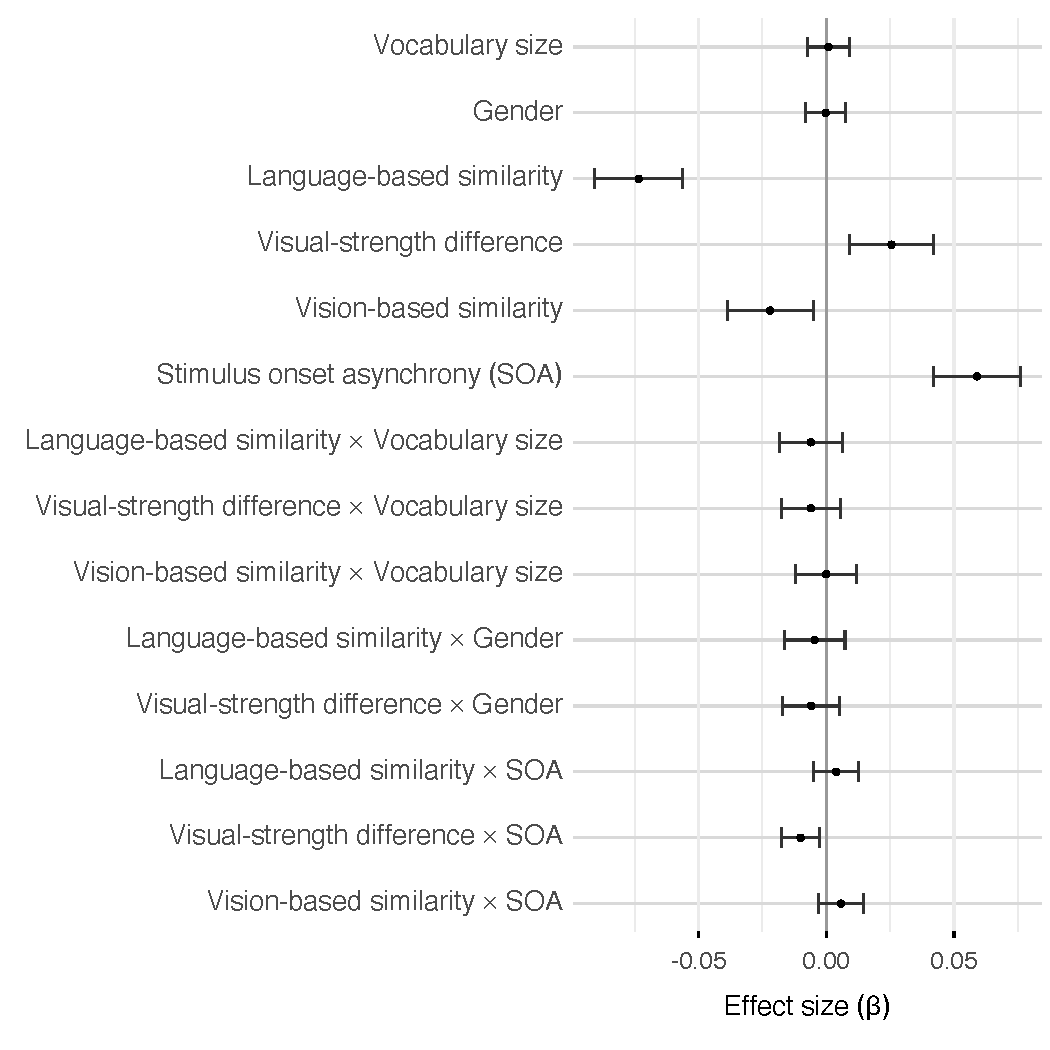
\includegraphics[width=0.89\linewidth]{/Users/pablodejuanbernabeu/Library/CloudStorage/OneDrive-LancasterUniversity/semanticpriming-semanticdecision-lexicaldecision/semanticpriming/analysis_with_visualsimilarity/plots/semanticpriming_with_visualsimilarity_confidence_intervals_plot} 

}

\caption{Means and 95\% confidence intervals for the effects of interest in the semantic priming model that included visual similarity.}\label{fig:semanticpriming-with-visualsimilarity-confidence-intervals-plot}
\end{figure}

The results revealed that visual-strength difference had a significantly larger effect. This difference was not due to an excessive collinearity between these measures (\(r\) = -0.04). Also importantly, both measures appeared to be valid based on their correlations with language-based similarity and with word concreteness.

\hypertarget{statistical-power-analysis}{%
\subsubsection{Statistical power analysis}\label{statistical-power-analysis}}

Power curves were performed for most effects of interest in the main model (no power analysis was performed for the model that included visual similarity). Figures \ref{fig:semanticpriming-powercurve-plots-1-2-3} and \ref{fig:semanticpriming-powercurve-plots-4-5-6-7-8-9} show the estimated power for the main effects and the interactions, respectively.

\begin{figure}

{\centering 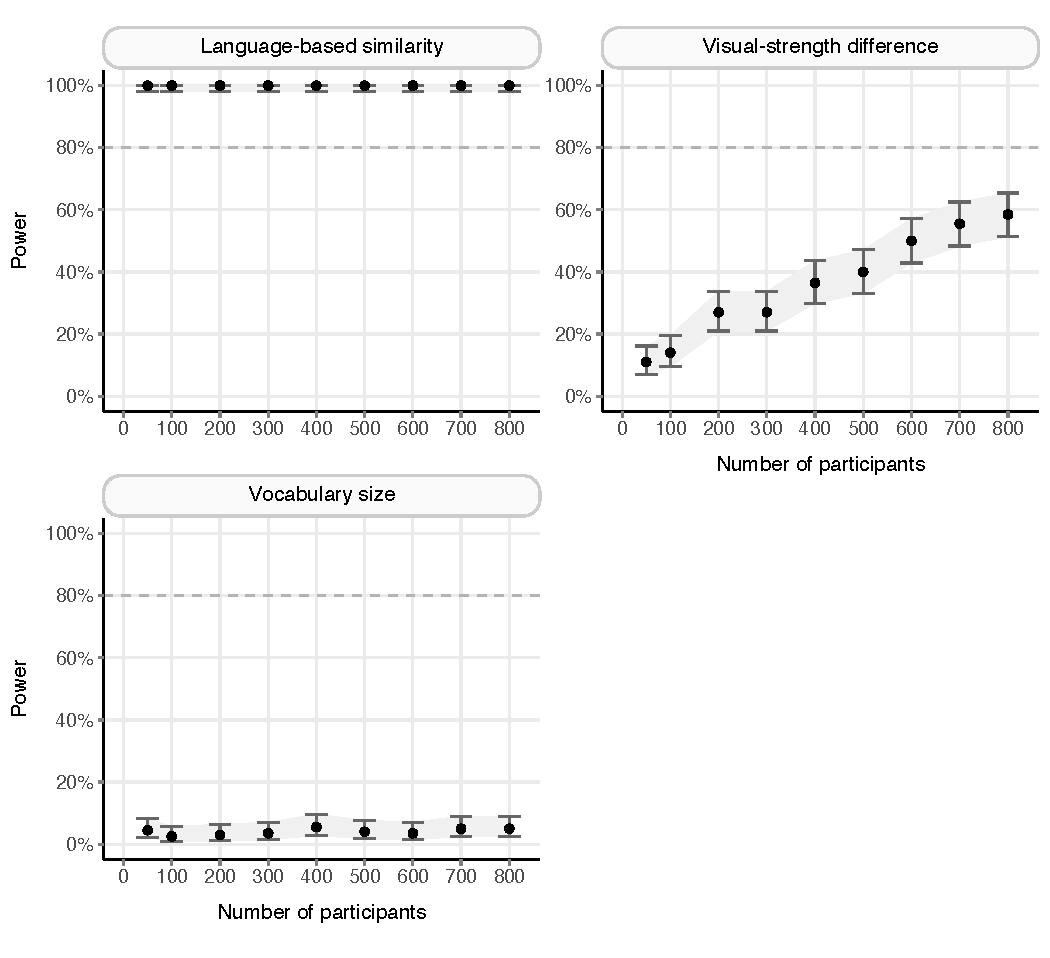
\includegraphics[width=1\linewidth]{/Users/pablodejuanbernabeu/Library/CloudStorage/OneDrive-LancasterUniversity/semanticpriming-semanticdecision-lexicaldecision/semanticpriming/power_analysis/plots/semanticpriming_powercurve_plots_1_2_3} 

}

\caption{Power curves for some main effects in the semantic priming study.}\label{fig:semanticpriming-powercurve-plots-1-2-3}
\end{figure}

\begin{figure}

{\centering 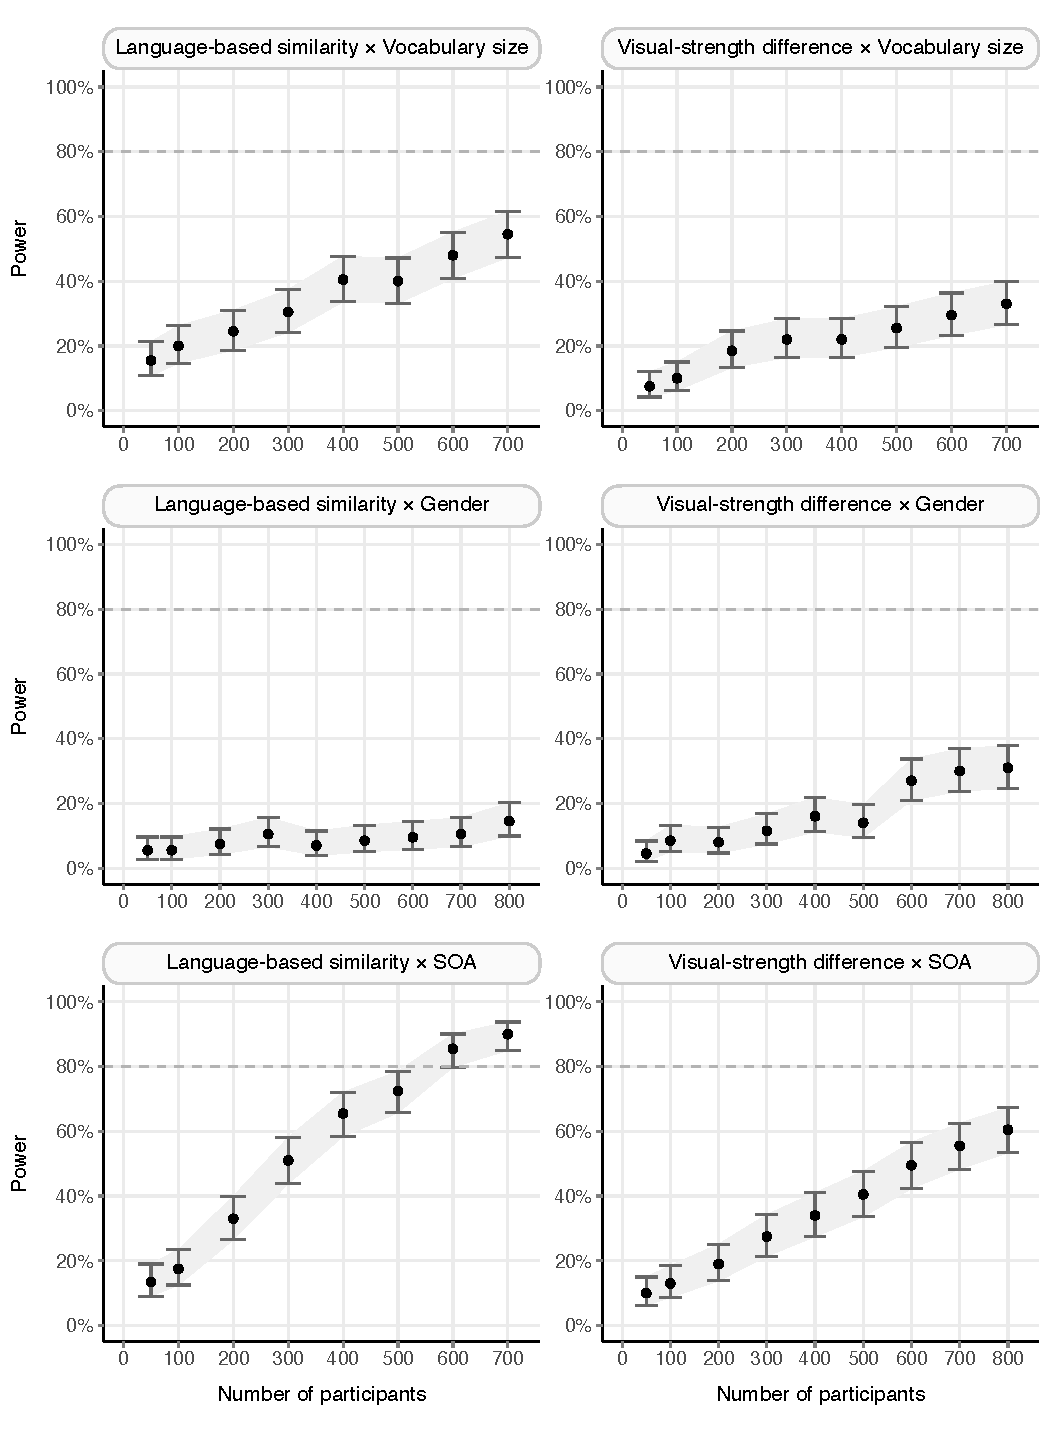
\includegraphics[width=0.9\linewidth]{/Users/pablodejuanbernabeu/Library/CloudStorage/OneDrive-LancasterUniversity/semanticpriming-semanticdecision-lexicaldecision/semanticpriming/power_analysis/plots/semanticpriming_powercurve_plots_4_5_6_7_8_9} 

}

\caption{Power curves for some interactions in the semantic priming study.}\label{fig:semanticpriming-powercurve-plots-4-5-6-7-8-9}
\end{figure}

\_\_\_\_\_\_\_ interpret \_\_\_\_\_\_\_\_\_\_\_\_

\hypertarget{discussion}{%
\subsection{Discussion}\label{discussion}}

\begin{center}\rule{0.5\linewidth}{0.5pt}\end{center}

\clearpage

\hypertarget{study-2-semantic-decision}{%
\section{Study 2: Semantic decision}\label{study-2-semantic-decision}}

The semantic decision task probes into the role of concreteness in conceptual processing. Specifically, this task requires participants to classify words as abstract or concrete. Researchers then analyse whether the responses can be explained by the sensory experientiality of the referents---that is, the degree to which they can be experienced through our senses---and by other variables, such as word frequency. The core data set in this study was that of the Calgary Semantic Decision Project (Pexman et al., 2017; Pexman \& Yap, 2018). The experimental task is semantic decision, in which participants judge whether words are relatively concrete (e.g., `building') or abstract (e.g., `thought').

Research has found that the processing of relatively concrete words relies considerably on sensorimotor information (Hultén et al., 2021; Kousta et al., 2011; Vigliocco et al., 2014). In contrast, the processing of relatively abstract words seems to draw more heavily on information from language (Barca et al., 2020; Duñabeitia et al., 2009; Snefjella \& Blank, 2020), emotion (Kousta et al., 2011; Ponari et al., 2020; Ponari, Norbury, Rotaru, et al., 2018; Ponari, Norbury, \& Vigliocco, 2018; Vigliocco et al., 2014) and sociality (Borghi et al., 2019; Diveica et al., 2022).

\hypertarget{word-co-occurrence}{%
\subsection{Word co-occurrence}\label{word-co-occurrence}}

Wingfield and Connell (2022) reanalysed the data from Pexman et al. (2017) using language-based variables that are more related to the language system than to the visual system. The authors found that the variables that best explained RTs were word co-occurrence measures. Specifically, the measures corresponded to the distance from each stimulus word to two labels that were central to the task, namely, the words `abstract' and `concrete'. Wingfield and Connell studied these distance measures in various forms, and found that cosine and correlation distance yielded the best results. We used the correlation distance following the advice of (Kiela \& Bottou, 2014). Furthermore, we sought to avoid the collinearity between these variables (\(r\) = .99) and to facilitate the analysis of interactions with other variables. For this purpose, we created a difference score by subtracting distance to `abstract' from the distance to `concrete'. The resulting variable was practically equivalent to the distance to `abstract', as attested by its large correlation with word concreteness (\(r\) = 0.02). Last, it should be noted that this difference score may not be affected by the reduced sensitivity of other ones (see Rodríguez-Ferreiro et al., 2020), as this difference score did not entail an aggregation of data points over any third variables.

\hypertarget{methods-2}{%
\subsection{Methods}\label{methods-2}}

\hypertarget{effects-of-interest-1}{%
\subsubsection{Effects of interest}\label{effects-of-interest-1}}

\begin{itemize}
\item
  Z-scored vocabulary size {[}\texttt{z\_vocabulary\_size}; calculated from \texttt{NAART} in Pexman et al. (2017){]}. In the test used by Pexman and Yap (2018), participants were presented with 35 rare words, whose pronunciations are not regular (e.g., \emph{gaoled}, \emph{ennui}), and they were asked to read the words aloud. When they pronounced a word correctly, it was inferred that they knew the word. This test was based on NAART35, a short version of the North American Adult Reading Test (Uttl, 2002).
\item
  Z-scored, recoded participant's gender {[}\texttt{z\_recoded\_participant\_gender}; calculated from \texttt{Gender} in Pexman and Yap (2018){]}
\item
  Z-scored distance to word `abstract': a distributional semantic distance measure obtained from Wingfield and Connell (2022) that reflects the correlation distance between each stimulus word and the word `abstract'.\footnote{Specifically, this measure is a difference score that merges both the distance to the word `abstract' and the distance to the word `concrete'. We drew on both variables because Wingfield and Connell (2022) found them to be similarly important. Yet, we had to create a difference score because these variables were highly correlated (\(r\) = .99), we created a difference score by subtracting the distance to `abstract' from the distance to `concrete'. The resulting difference score was practically equivalent to the distance to the word `abstract', as attested by its correlation with word concreteness (see Figure \ref{fig:semanticdecision-correlations}). Our difference score in practice The variable \texttt{Conditional\_probability\_BNC\_r5\_correlation\_abstract\_distance} was subtracted from \texttt{Conditional\_probability\_BNC\_r5\_correlation\_concrete\_distance}.}
\item
  Z-scored vision-based information in words {[}\texttt{z\_visual\_rating}; calculated from \texttt{Visual.mean} in Lynott et al. (2020){]}
\end{itemize}

The final data set contained 306 participants, 8,927 words, and a total of 246,432 RTs. On average, there were 755 words per participant (\(SD\) = 42.05), and conversely, 26 participants per word (\(SD\) = 4.80).

Figure \ref{fig:semanticdecision-correlations} shows the zero-order correlations among the predictors among the predictors and the dependent variable.

\begin{figure}

{\centering 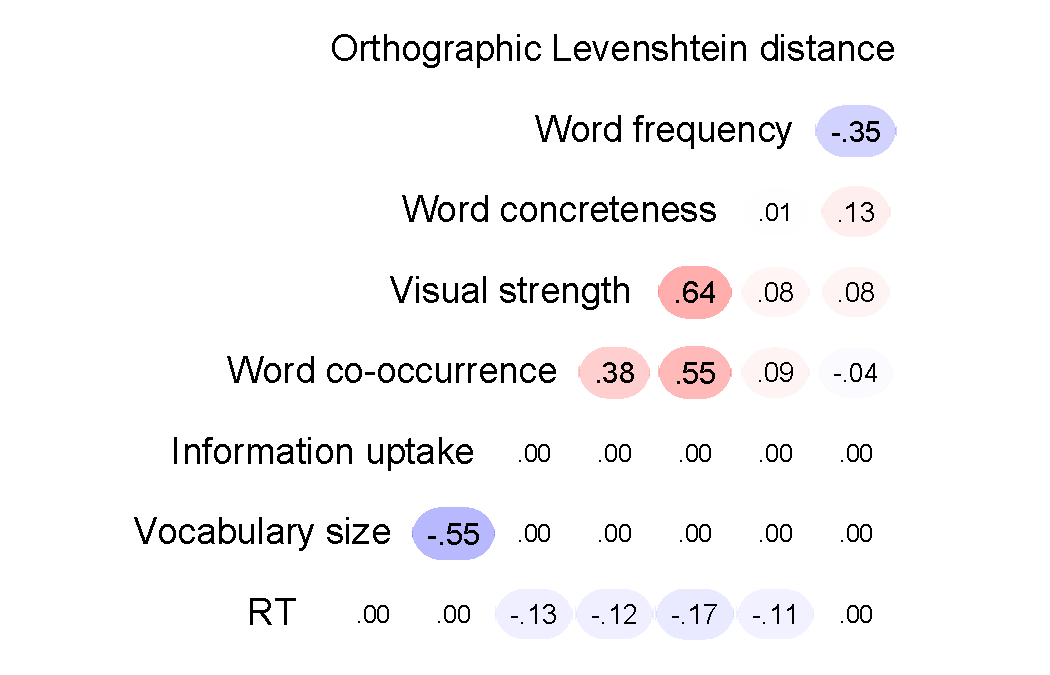
\includegraphics[width=0.57\linewidth]{manuscript_files/figure-latex/semanticdecision-correlations-1} 

}

\caption{Zero-order correlations in the semantic decision study.}\label{fig:semanticdecision-correlations}
\end{figure}

\hypertarget{covariates-1}{%
\subsubsection{Covariates}\label{covariates-1}}

The following covariates were included in the model to allow a rigorous analysis of the effects of interest.

\begin{itemize}
\item
  Lexical (see \protect\hyperlink{appendix-A-lexical-covariates}{\underline{Appendix A}}): z-scored word frequency and orthographic Levenshtein distance (Balota et al., 2007)
\item
  Semantic: z-scored word concreteness (Brysbaert et al., 2014). This variable is used as a covariate of visual strength, and it is especially fundamental in the semantic decision task, in which participants judge whether words are concrete or abstract (for a more general consideration of concreteness, see Bottini et al., 2021). Indeed, owing to the instructions of the task, word concreteness is likely to be more relevant to the participants' task than our effects of interest.
\item
  Individual differences: z-scored information uptake (Pexman \& Yap, 2018). This covariate is related to vocabulary size (Ratcliff et al., 2010; also see James et al., 2018; Pexman \& Yap, 2018).
\end{itemize}

\hypertarget{diagnostics-for-the-frequentist-model-2}{%
\subsubsection{Diagnostics for the frequentist model}\label{diagnostics-for-the-frequentist-model-2}}

The model presented convergence warnings. To avoid removing important random slopes, which could increase the Type I error (Brauer \& Curtin, 2018; Singmann \& Kellen, 2019), we examined the model after refitting it using seven optimization algorithms through the `allFit' function of the `lme4' package (Bates et al., 2021). The results showed that all optimizers produced virtually identical means for all effects, suggesting that the convergence warnings were not consequential {[}Bates et al. (2021); see \protect\hyperlink{appendix-B-frequentist-analysis-diagnostics}{\underline{Appendix B}}{]}.

The residual errors were not normally distributed, and attempts to mitigate this deviation proved unsuccessful (see \protect\hyperlink{appendix-B-frequentist-analysis-diagnostics}{\underline{Appendix B}}). However, this is not likely to have posed a major problem, as mixed-effects models are fairly robust to deviations from normality (Knief \& Forstmeier, 2021; Schielzeth et al., 2020).

The model did not present multicollinearity problems, all VIFs being smaller than 2 (Dormann et al., 2013; Harrison et al., 2018).

\hypertarget{diagnostics-for-the-bayesian-model-1}{%
\subsubsection{Diagnostics for the Bayesian model}\label{diagnostics-for-the-bayesian-model-1}}

Three Bayesian models were run that were respectively characterised by informative, weakly-informative and diffuse priors. In each model, 16 chains were used. In each chain, 2,000 warmup iterations were run, followed by 6,000 post-warmup iterations. Thus, a total of 96,000 post-warmup draws were produced over all the chains.

The maximum \(\widehat R\) value for the fixed effects across the three models was 1.42, far exceeding the 1.01 threshold (Vehtari et al., 2021; also see Schoot et al., 2021). Similarly, the maximum \(\widehat R\) value for the random effects was 1.31. Furthermore, the posterior predictive checks revealed major divergences between the observed data and the predicted outcome (see \protect\hyperlink{appendix-C-Bayesian-analysis-diagnostics}{\underline{Appendix C}}). Since the results were not valid, they are not shown in the main text but instead in \protect\hyperlink{appendix-E-Bayesian-analysis-results}{\underline{Appendix E}}.

\hypertarget{results-1}{%
\subsection{Results}\label{results-1}}

Table \ref{tab:semanticdecision-frequentist-model} presents the results of the mixed-effects model.

\begin{table}[!h]

\caption{\label{tab:semanticdecision-frequentist-model}Frequentist model for the semantic decision study.}
\centering
\begin{threeparttable}
\begin{tabular}[t]{lrrrrr}
\toprule
\multicolumn{1}{c}{ } & \multicolumn{1}{c}{$\upbeta$} & \multicolumn{1}{c}{$SE$} & \multicolumn{1}{c}{95\% CI} & \multicolumn{1}{c}{$t$} & \multicolumn{1}{c}{$p$}\\
\midrule
(Intercept) & 0.05 & 0.00 & {}[0.04, 0.06] & 11.87 & <.001\\
\addlinespace[0.3em]
\multicolumn{6}{l}{\textbf{Individual differences}}\\
\cellcolor{gray!6}{\hspace{1em}Information uptake} & \cellcolor{gray!6}{0.00} & \cellcolor{gray!6}{0.00} & \cellcolor{gray!6}{{}[0.00, 0.00]} & \cellcolor{gray!6}{0.20} & \cellcolor{gray!6}{.844}\\
\hspace{1em}Vocabulary size $^{\text{a}}$ & 0.00 & 0.00 & {}[-0.01, 0.00] & -1.42 & .155\\
\hspace{1em}Gender $^{\text{a}}$ & 0.00 & 0.00 & {}[0.00, 0.00] & -0.47 & .636\\
\addlinespace[0.3em]
\multicolumn{6}{l}{\textbf{Lexical covariates}}\\
\cellcolor{gray!6}{\hspace{1em}Word frequency} & \cellcolor{gray!6}{-0.12} & \cellcolor{gray!6}{0.00} & \cellcolor{gray!6}{{}[-0.13, -0.12]} & \cellcolor{gray!6}{-28.63} & \cellcolor{gray!6}{<.001}\\
\cellcolor{gray!6}{\hspace{1em}Orthographic Levenshtein distance} & \cellcolor{gray!6}{-0.01} & \cellcolor{gray!6}{0.00} & \cellcolor{gray!6}{{}[-0.02, 0.00]} & \cellcolor{gray!6}{-3.05} & \cellcolor{gray!6}{.002}\\
\addlinespace[0.3em]
\multicolumn{6}{l}{\textbf{Semantic variables}}\\
\cellcolor{gray!6}{\hspace{1em}Word concreteness} & \cellcolor{gray!6}{-0.13} & \cellcolor{gray!6}{0.01} & \cellcolor{gray!6}{{}[-0.14, -0.11]} & \cellcolor{gray!6}{-21.39} & \cellcolor{gray!6}{<.001}\\
\hspace{1em}Distance to word 'abstract' $^{\text{b}}$ & -0.03 & 0.01 & {}[-0.04, -0.02] & -4.48 & <.001\\
\hspace{1em}Visual strength $^{\text{b}}$ & -0.02 & 0.01 & {}[-0.03, -0.01] & -2.91 & .004\\
\addlinespace[0.3em]
\multicolumn{6}{l}{\textbf{Interactions}}\\
\cellcolor{gray!6}{\hspace{1em}Word concreteness  $\times$  Gender} & \cellcolor{gray!6}{-0.01} & \cellcolor{gray!6}{0.00} & \cellcolor{gray!6}{{}[-0.02, 0.00]} & \cellcolor{gray!6}{-3.50} & \cellcolor{gray!6}{<.001}\\
\cellcolor{gray!6}{\hspace{1em}Visual strength  $\times$  Information uptake} & \cellcolor{gray!6}{0.02} & \cellcolor{gray!6}{0.01} & \cellcolor{gray!6}{{}[0.01, 0.03]} & \cellcolor{gray!6}{3.05} & \cellcolor{gray!6}{.003}\\
\hspace{1em}\makecell[l]{Distance to word 'abstract'  $\times$ \\ \hspace{0.3cm} Vocabulary size} & 0.01 & 0.01 & {}[0.00, 0.02] & 1.66 & .098\\
\hspace{1em}Visual strength  $\times$  Vocabulary size & 0.01 & 0.01 & {}[0.00, 0.02] & 2.03 & .043\\
\hspace{1em}Distance to word 'abstract'  $\times$  Gender & 0.00 & 0.00 & {}[-0.01, 0.01] & 0.86 & .393\\
\hspace{1em}Visual strength  $\times$  Gender & 0.00 & 0.00 & {}[-0.01, 0.01] & -0.08 & .940\\
\hspace{1em}Word concreteness  $\times$  Vocabulary size & -0.02 & 0.00 & {}[-0.03, -0.02] & -7.66 & <.001\\
\hspace{1em}\makecell[l]{Information uptake  $\times$ \\ \hspace{0.3cm} Distance to word 'abstract'} & 0.01 & 0.01 & {}[0.00, 0.02] & 1.48 & .141\\
\bottomrule
\end{tabular}
\begin{tablenotes}
\item \textit{\linebreak} 
\item \textit{Note}. $\upbeta$ = Estimate based on z-scored variables; \textit{SE} = standard error; \linebreak \phantom{.}CI = confidence interval. Shaded rows contain covariates. Some interactions are \linebreak \phantom{.}split over two lines, with the second line indented. \linebreak \linebreak \phantom{.}$^{\text{a}}$ By-word random slopes were included for this effect. \linebreak \phantom{.}$^{\text{b}}$ By-participant random slopes were included for this effect.
\end{tablenotes}
\end{threeparttable}
\end{table}

The fixed effects of this model explained 4.11\% of the variance, and the random effects explained 17.48\% (Nakagawa et al., 2017).

Figures \ref{fig:semanticdecision-interactions-with-vocabulary-size}-a and \ref{fig:semanticdecision-interactions-with-vocabulary-size}-b show that lower-vocabulary participants benefited more strongly than higher-vocabulary participants from both language- and vision-based similarity. In contrast, Figure \ref{fig:semanticdecision-interactions-with-vocabulary-size}-c shows that higher-vocabulary participants benefitted more strongly from word concreteness. Since the variable that is most relevant to the semantic decision task is word concreteness, the present interactions may suggest that higher-vocabulary participants were better able to focus on the most relevant information, whereas lower-vocabulary participants were sensitive to a greater breadth of information (Lim et al., 2020; Pexman \& Yap, 2018; Yap et al., 2012, 2017).



\begin{figure}

{\centering 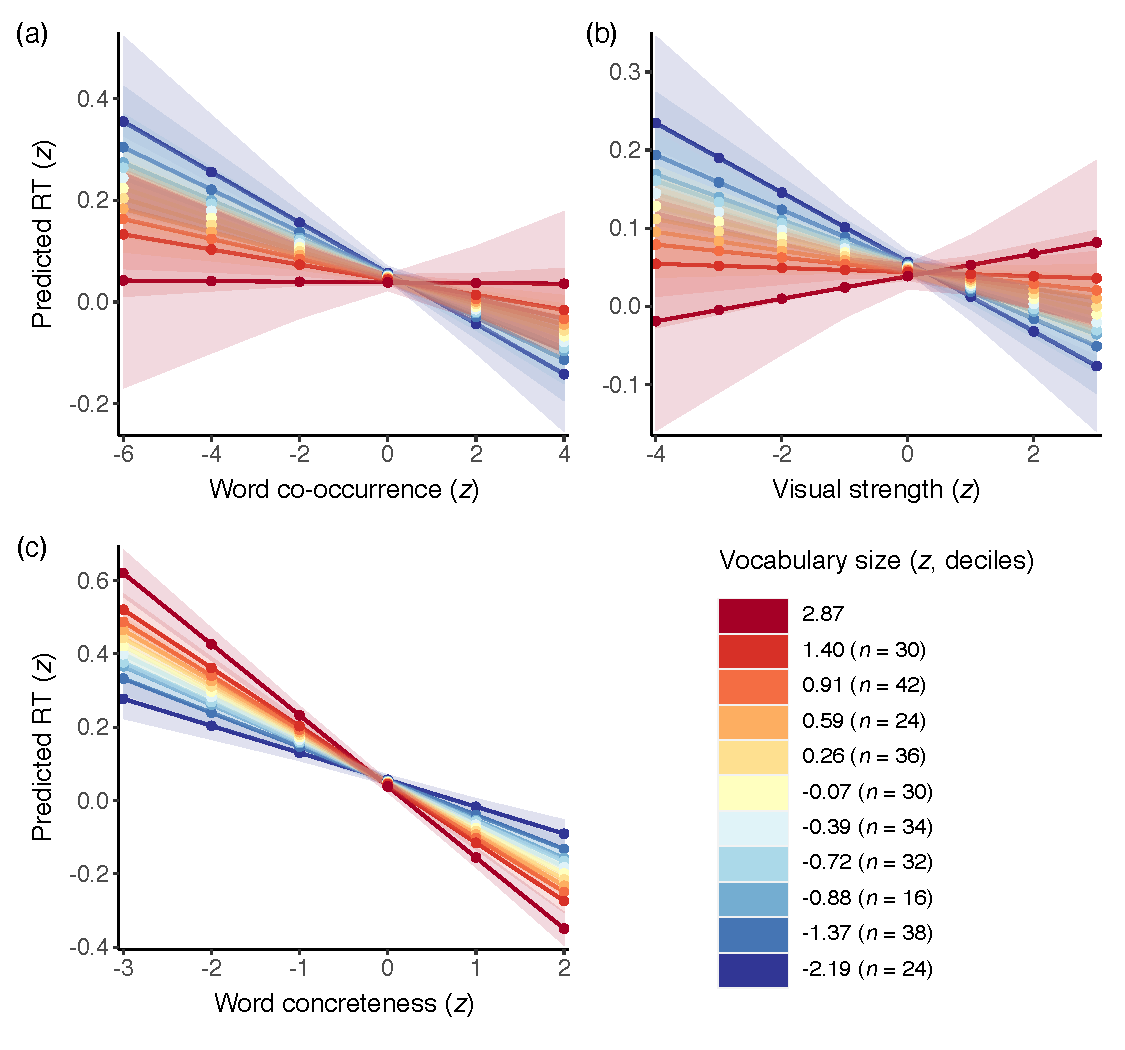
\includegraphics[width=1\linewidth,height=0.95\textheight]{/Users/pablodejuanbernabeu/Library/CloudStorage/OneDrive-LancasterUniversity/semanticpriming-semanticdecision-lexicaldecision/semanticdecision/frequentist_analysis/plots/semanticdecision-interactions-with-vocabulary-size} 

}

\caption{Interactions of vocabulary size with (a) language-based information, (b) visual strength and (c) word concreteness. Vocabulary size is constrained to deciles, whereas in the statistical analysis it contained more values within the current range. \emph{n} = number of participants contained between decile values.}\label{fig:semanticdecision-interactions-with-vocabulary-size}
\end{figure}

The present analysis uses a continuous measure of word concreteness. In contrast, Pexman and Yap (2018) analysed the same data set after dividing the stimulus words into abstract and concrete subsets, which they analysed separately. Pexman and Yap found that high-vocabulary participants were more sensitive to the relative abstractness of words. Specifically, these participants were faster to classify very abstract words than mid-abstract ones, thus presenting a reverse concreteness effect. Such a reverse effect might stem from the bimodal distributions of concreteness ratings (Brysbaert et al., 2014) and semantic decisions (Pexman \& Yap, 2018). The reverse effect has also been found in semantic dementia patients (Connell \& Lynott, 2012). Since the reverse effect contrasted with the long-established concreteness effect, the former has sometimes been regarded as an inconsistency.

Notwithstanding the aforementioned bimodal distributions, Troche et al. (2017) suggested that a continuous analysis remains necessary to study word concreteness (also see Cohen, 1983). Consistent with this, our present findings demonstrated the sensitivity of a continuous word-concreteness variable to patterns such as the greater role of task-relevant variables in high-vocabulary participants. In conclusion, the literature and our findings suggest that the split-data approach and the continuous approach to word concreteness are both useful. Where feasible, the application of both approaches would provide the most information.

\hypertarget{visualising-the-estimates-1}{%
\subsubsection{Visualising the estimates}\label{visualising-the-estimates-1}}

Figure \ref{fig:semanticdecision-confidence-intervals-plot} presents the means and 95\% confidence intervals for the effects of interest.\footnote{Bayesian estimates not shown as they were not valid. They are nonetheless available in \protect\hyperlink{appendix-E-Bayesian-analysis-results}{\underline{Appendix E}}.}

\begin{figure}

{\centering 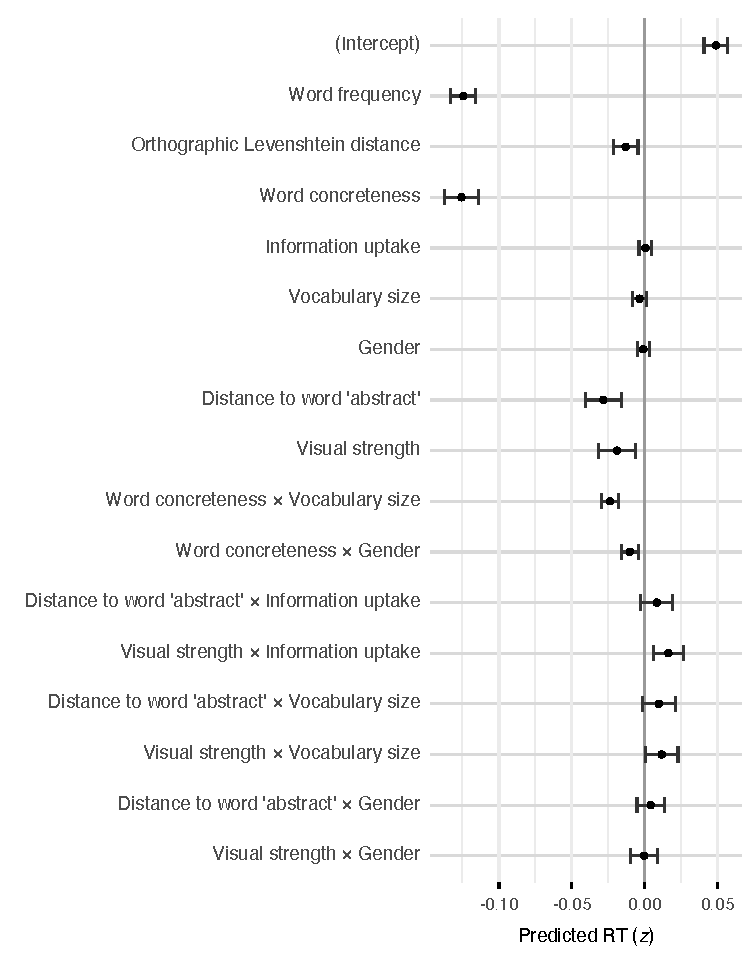
\includegraphics[width=0.92\linewidth]{/Users/pablodejuanbernabeu/Library/CloudStorage/OneDrive-LancasterUniversity/semanticpriming-semanticdecision-lexicaldecision/semanticdecision/frequentist_analysis/plots/semanticdecision_confidence_intervals_plot} 

}

\caption{Means and 95\% confidence intervals for the effects of interest in the semantic decision model.}\label{fig:semanticdecision-confidence-intervals-plot}
\end{figure}

\hypertarget{statistical-power-analysis-1}{%
\subsubsection{Statistical power analysis}\label{statistical-power-analysis-1}}

Figures \ref{fig:semanticdecision-powercurve-plots-1-2-3} and \ref{fig:semanticdecision-powercurve-plots-4-5-6-7} show the estimated power available for main effects and interactions of interest, respectively.

\begin{figure}

{\centering 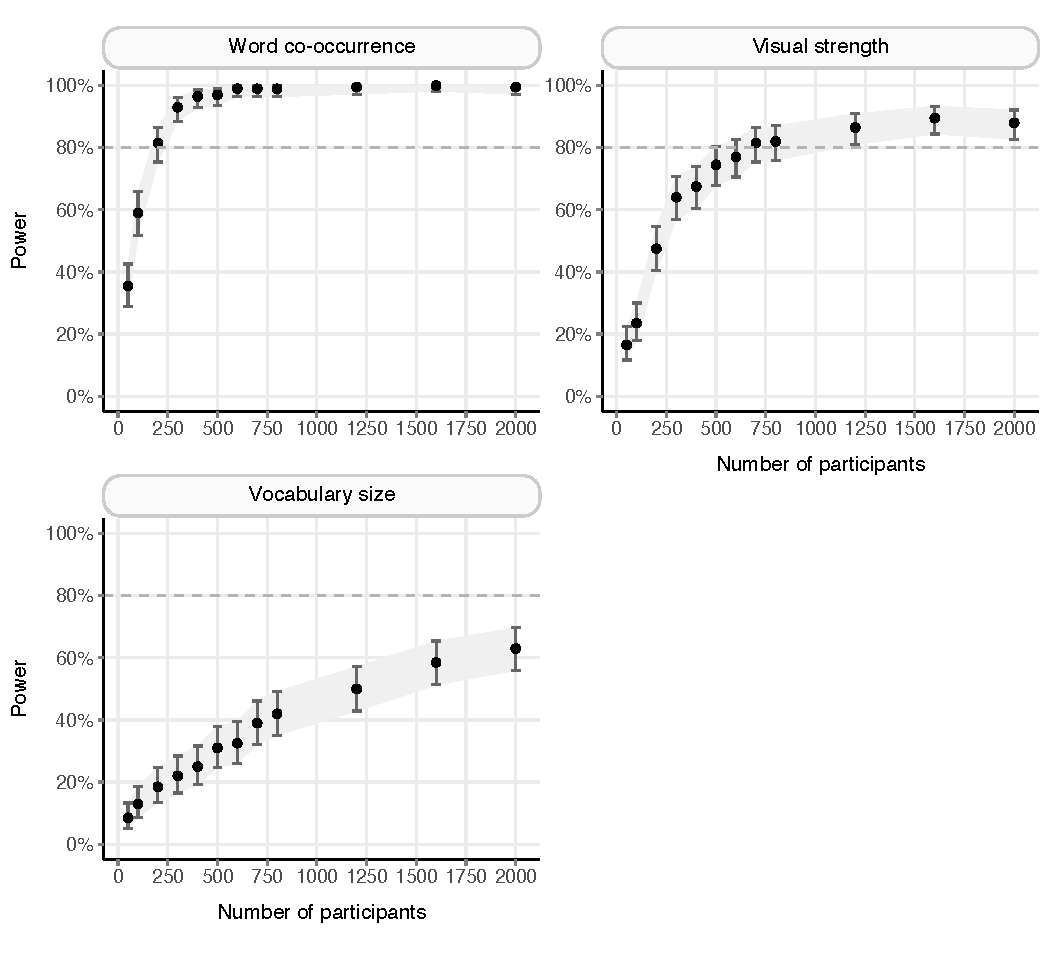
\includegraphics[width=1\linewidth]{/Users/pablodejuanbernabeu/Library/CloudStorage/OneDrive-LancasterUniversity/semanticpriming-semanticdecision-lexicaldecision/semanticdecision/power_analysis/plots/semanticdecision_powercurve_plots_1_2_3} 

}

\caption{Power curves for some main effects in the semantic decision study.}\label{fig:semanticdecision-powercurve-plots-1-2-3}
\end{figure}

\begin{figure}

{\centering 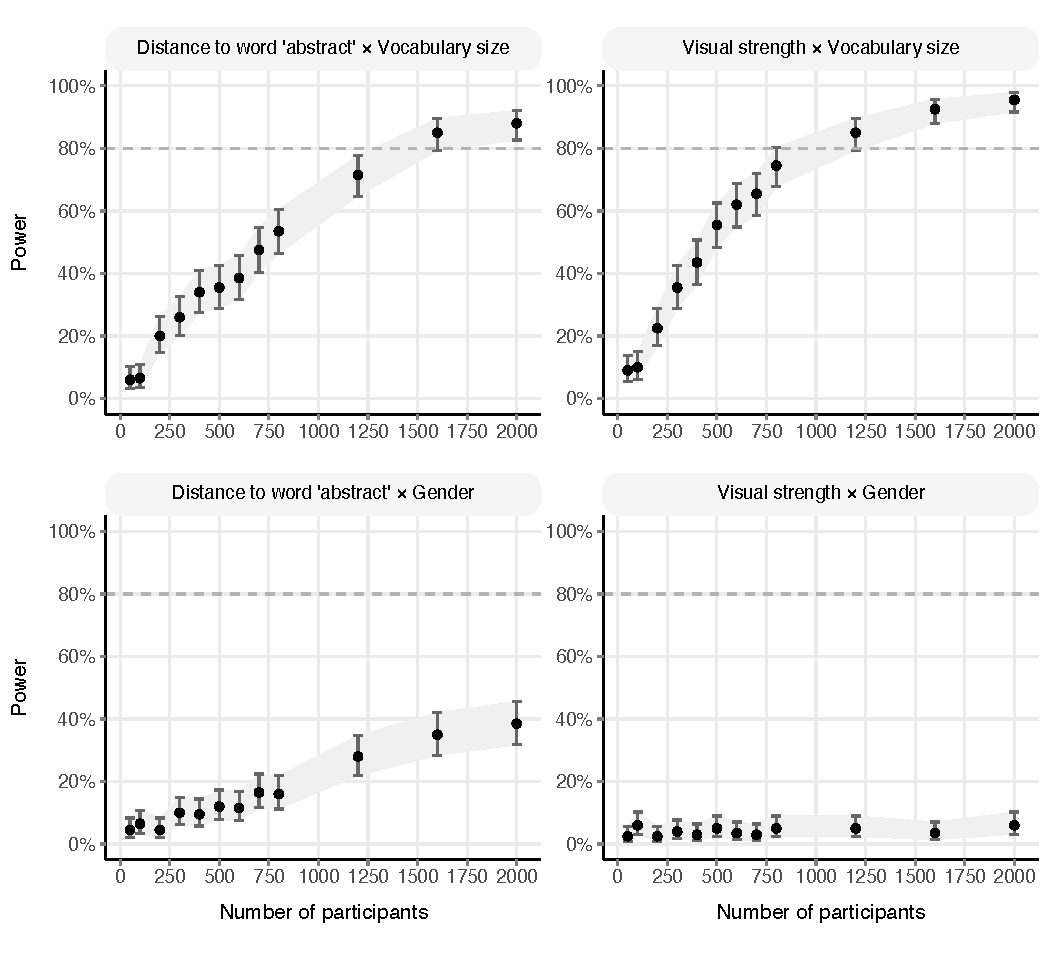
\includegraphics[width=1\linewidth]{/Users/pablodejuanbernabeu/Library/CloudStorage/OneDrive-LancasterUniversity/semanticpriming-semanticdecision-lexicaldecision/semanticdecision/power_analysis/plots/semanticdecision_powercurve_plots_4_5_6_7} 

}

\caption{Power curves for some interactions in the semantic decision study.}\label{fig:semanticdecision-powercurve-plots-4-5-6-7}
\end{figure}

\_\_\_\_\_\_\_ interpret \_\_\_\_\_\_\_\_\_\_\_\_

\hypertarget{discussion-1}{%
\subsection{Discussion}\label{discussion-1}}

\begin{center}\rule{0.5\linewidth}{0.5pt}\end{center}

\clearpage

\hypertarget{study-3-lexical-decision}{%
\section{Study 3: Lexical decision}\label{study-3-lexical-decision}}

The core data set in this study was the lexical decision subset of the English Lexicon Project---ELP (Balota et al., 2007). The lexical decision task differs from semantic priming and semantic decision in two important aspects.

\begin{enumerate}
\def\labelenumi{\arabic{enumi}.}
\item
  \textbf{Less semantic processing.} The lexical decision paradigm is likely to involve less semantic processing than the other paradigms. \_\_\_\_\_\_\_\_\_\_\_\_
\item
  \textbf{Single-word measures.} Compared to semantic priming and semantic decision, it is more difficult in the lexical decision paradigm to create word-to-word distance measures to capture language-based and vision-based information. The possibility of calculating the distance between words in consecutive trials is hindered by the need to skip trials, owing to the high prevalence of nonword trials in the lexical decision paradigm. Therefore, the measures must be based on each word alone. Accordingly, vision-based information can be operationalised as the visual strength of each word. Language-based information could be operationalised as any of several lexical variables. In the present study, word frequency was chosen as it had the most explanatory power out of 5 candidates---the other candidates being number of letters, number of syllables, orthographic Levenshtein distance and phonological Levenshtein distance (see \protect\hyperlink{appendix-A-lexical-covariates}{\underline{Appendix A}}). It should also be noted that word frequency has been found to be more closely related to semantic variables than to lexical ones, such as word length, orthography, phonology (see Table 4 in Yap et al., 2012).
\end{enumerate}

Word frequency is also of interest due to its varying relationship to vocabulary size across different paradigms. Yap et al. (2012) found that higher-vocabulary participants in the ELP were more strongly influenced by word frequency than lower-vocabulary participants. The same finding also appeared in a lexical decision study in Chinese (Lim et al., 2020). In contrast, deeper semantic tasks, such as semantic priming (Yap et al., 2017) and semantic decision (Pexman \& Yap, 2018), have yielded the opposite pattern, with the effect of word frequency decreasing in higher-vocabulary participants.

\hypertarget{effects-of-interest-2}{%
\subsection{Effects of interest}\label{effects-of-interest-2}}

\begin{itemize}
\item
  Z-scored vocabulary age {[}\texttt{z\_vocabulary\_age}; calculated from \texttt{vocabAge} in Balota et al. (2007){]}
\item
  Z-scored, recoded participant's gender {[}\texttt{z\_recoded\_participant\_gender}; calculated from \texttt{Gender} in Balota et al. (2007){]}
\item
  Z-scored word frequency {[}\texttt{z\_word\_frequency}; calculated from \texttt{LgSUBTLWF} in Balota et al. (2007){]}
\item
  Z-scored vision-based information in words {[}\texttt{z\_visual\_rating}; calculated from \texttt{Visual.mean} in Lynott et al. (2020){]}
\end{itemize}

The final data set contained 795 participants, 12,636 words, and a total of 19,828 RTs. On average, there were 25 words per participant (\(SD\) = 36.04), and conversely, 2 participants per word (\(SD\) = 0.86).

Figure \ref{fig:lexicaldecision-correlations} shows the zero-order correlations among the predictors and the dependent variable.

\begin{figure}

{\centering 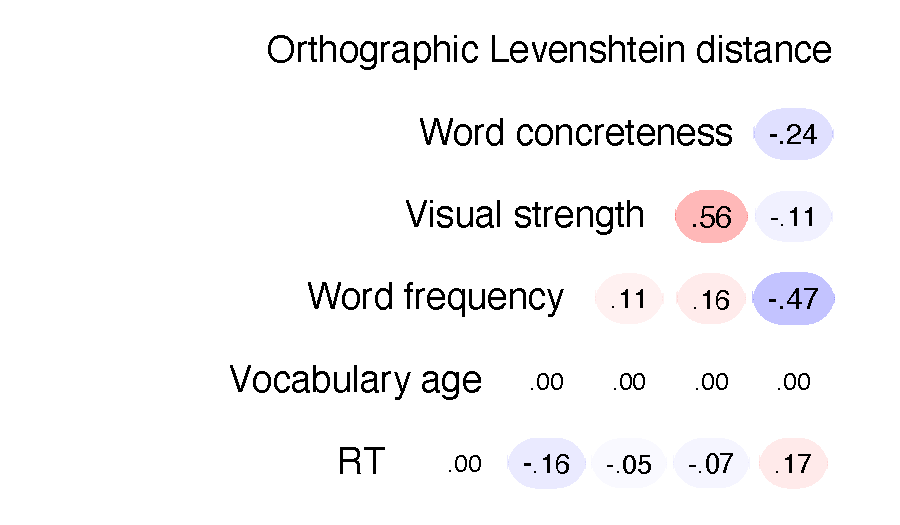
\includegraphics[width=0.5\linewidth]{manuscript_files/figure-latex/lexicaldecision-correlations-1} 

}

\caption{Zero-order correlations in the lexical decision study.}\label{fig:lexicaldecision-correlations}
\end{figure}

\hypertarget{covariates-2}{%
\subsection{Covariates}\label{covariates-2}}

The following lexical covariates were included in the model to allow a rigorous analysis of the effects of interest.

\begin{itemize}
\item
  Lexical (see \protect\hyperlink{appendix-A-lexical-covariates}{\underline{Appendix A}}): Z-scored orthographic Levenshtein distance (Balota et al., 2007)
\item
  Semantic: z-scored word concreteness (Brysbaert et al., 2014), used as a covariate of visual rating.
\end{itemize}

\hypertarget{diagnostics-for-the-frequentist-model-3}{%
\subsubsection{Diagnostics for the frequentist model}\label{diagnostics-for-the-frequentist-model-3}}

The model presented convergence warnings. To avoid removing important random slopes, which could increase the Type I error (Brauer \& Curtin, 2018; Singmann \& Kellen, 2019), we examined the model after refitting it using seven optimization algorithms through the `allFit' function of the `lme4' package (Bates et al., 2021). The results showed that all optimizers produced virtually identical means for all effects, suggesting that the convergence warnings were not consequential {[}Bates et al. (2021); see \protect\hyperlink{appendix-B-frequentist-analysis-diagnostics}{\underline{Appendix B}}{]}.

The residual errors were not normally distributed, and attempts to mitigate this deviation proved unsuccessful (see \protect\hyperlink{appendix-B-frequentist-analysis-diagnostics}{\underline{Appendix B}}). However, this is not likely to have posed a major problem, as mixed-effects models are fairly robust to deviations from normality (Knief \& Forstmeier, 2021; Schielzeth et al., 2020).

The model did not present multicollinearity problems, all VIFs being smaller than 2 (Dormann et al., 2013; Harrison et al., 2018).

\hypertarget{diagnostics-for-the-bayesian-model-2}{%
\subsubsection{Diagnostics for the Bayesian model}\label{diagnostics-for-the-bayesian-model-2}}

Three Bayesian models were run that were respectively characterised by informative, weakly-informative and diffuse priors. In each model, 5 chains were used. In each chain, 2,000 warmup iterations were run, followed by 18,000 post-warmup iterations. Thus, a total of 90,000 post-warmup draws were produced over all the chains.

The maximum \(\widehat R\) value for the fixed effects across the three models was 1.00, suggesting that these effects converged (Schoot et al., 2021; Vehtari et al., 2021). For the random effects, the maximum \(\widehat R\) value was 1.02, barely exceeding the 1.01 threshold (Vehtari et al., 2021).

The posterior predictive checks were sound (see \protect\hyperlink{appendix-C-Bayesian-analysis-diagnostics}{\underline{Appendix C}}). Furthermore, in the prior sensitivity analysis, the results were virtually identical with the three priors that were considered (to recall the priors, see Figure \ref{fig:bayesian-priors} above; to view the results in detail, see \protect\hyperlink{appendix-E-Bayesian-analysis-results}{\underline{Appendix E}}).

\hypertarget{results-2}{%
\subsection{Results}\label{results-2}}

Table \ref{tab:lexicaldecision-frequentist-model} presents the results of the mixed-effects model.

\begin{table}[H]

\caption{\label{tab:lexicaldecision-frequentist-model}Frequentist model for the lexical decision study.}
\centering
\begin{threeparttable}
\begin{tabular}[t]{lrrrrr}
\toprule
\multicolumn{1}{c}{ } & \multicolumn{1}{c}{$\upbeta$} & \multicolumn{1}{c}{$SE$} & \multicolumn{1}{c}{95\% CI} & \multicolumn{1}{c}{$t$} & \multicolumn{1}{c}{$p$}\\
\midrule
(Intercept) & 0.00 & 0.01 & {}[-0.01, 0.01] & -0.02 & .983\\
\addlinespace[0.3em]
\multicolumn{6}{l}{\textbf{Individual differences}}\\
\hspace{1em}Vocabulary age $^{\text{a}}$ & 0.00 & 0.01 & {}[-0.01, 0.01] & -0.06 & .950\\
\hspace{1em}Gender $^{\text{a}}$ & 0.00 & 0.01 & {}[-0.01, 0.01] & 0.01 & .995\\
\addlinespace[0.3em]
\multicolumn{6}{l}{\textbf{Lexical covariate}}\\
\cellcolor{gray!6}{\hspace{1em}Orthographic Levenshtein distance} & \cellcolor{gray!6}{0.11} & \cellcolor{gray!6}{0.01} & \cellcolor{gray!6}{{}[0.09, 0.12]} & \cellcolor{gray!6}{13.41} & \cellcolor{gray!6}{<.001}\\
\addlinespace[0.3em]
\multicolumn{6}{l}{\textbf{Semantic variables}}\\
\cellcolor{gray!6}{\hspace{1em}Word concreteness} & \cellcolor{gray!6}{-0.02} & \cellcolor{gray!6}{0.01} & \cellcolor{gray!6}{{}[-0.04, -0.01]} & \cellcolor{gray!6}{-2.79} & \cellcolor{gray!6}{.005}\\
\hspace{1em}Word frequency $^{\text{b}}$ & -0.16 & 0.01 & {}[-0.18, -0.14] & -13.01 & <.001\\
\hspace{1em}Visual strength $^{\text{b}}$ & -0.01 & 0.01 & {}[-0.03, 0.01] & -1.36 & .175\\
\addlinespace[0.3em]
\multicolumn{6}{l}{\textbf{Interactions}}\\
\cellcolor{gray!6}{\hspace{1em}Word concreteness  $\times$  Vocabulary age} & \cellcolor{gray!6}{0.01} & \cellcolor{gray!6}{0.01} & \cellcolor{gray!6}{{}[-0.01, 0.03]} & \cellcolor{gray!6}{1.16} & \cellcolor{gray!6}{.244}\\
\cellcolor{gray!6}{\hspace{1em}Word concreteness  $\times$  Gender} & \cellcolor{gray!6}{0.00} & \cellcolor{gray!6}{0.01} & \cellcolor{gray!6}{{}[-0.02, 0.02]} & \cellcolor{gray!6}{0.16} & \cellcolor{gray!6}{.876}\\
\hspace{1em}Word frequency  $\times$  Vocabulary age & -0.02 & 0.01 & {}[-0.04, 0.01] & -1.31 & .191\\
\hspace{1em}Visual strength  $\times$  Vocabulary age & 0.00 & 0.01 & {}[-0.02, 0.02] & 0.05 & .962\\
\hspace{1em}Word frequency  $\times$  Gender & -0.02 & 0.01 & {}[-0.04, 0.00] & -1.75 & .080\\
\hspace{1em}Visual strength  $\times$  Gender & -0.01 & 0.01 & {}[-0.03, 0.01] & -0.86 & .390\\
\bottomrule
\end{tabular}
\begin{tablenotes}
\item \textit{\linebreak} 
\item \textit{Note}. $\upbeta$ = Estimate based on z-scored variables; \textit{SE} = standard error; \linebreak \phantom{.}CI = confidence interval. Shaded rows contain covariates. \linebreak \linebreak \phantom{.}$^{\text{a}}$ By-word random slopes were included for this effect. \linebreak \phantom{.}$^{\text{b}}$ By-participant random slopes were included for this effect.
\end{tablenotes}
\end{threeparttable}
\end{table}

The fixed effects of this model explained 5.61\% of the variance, and the random effects explained 10.25\% (Nakagawa et al., 2017).

\hypertarget{visualising-the-estimates-2}{%
\subsubsection{Visualising the estimates}\label{visualising-the-estimates-2}}

Figure \ref{fig:lexicaldecision-frequentist-bayesian-plot-weaklyinformativepriors-exgaussian} presents the posterior distribution of each effect, based on the informative prior model (for the models with the other priors, see \protect\hyperlink{appendix-E-Bayesian-analysis-results}{\underline{Appendix E}}). The frequentist estimates are also shown to facilitate the comparison with them.

\begin{figure}

{\centering 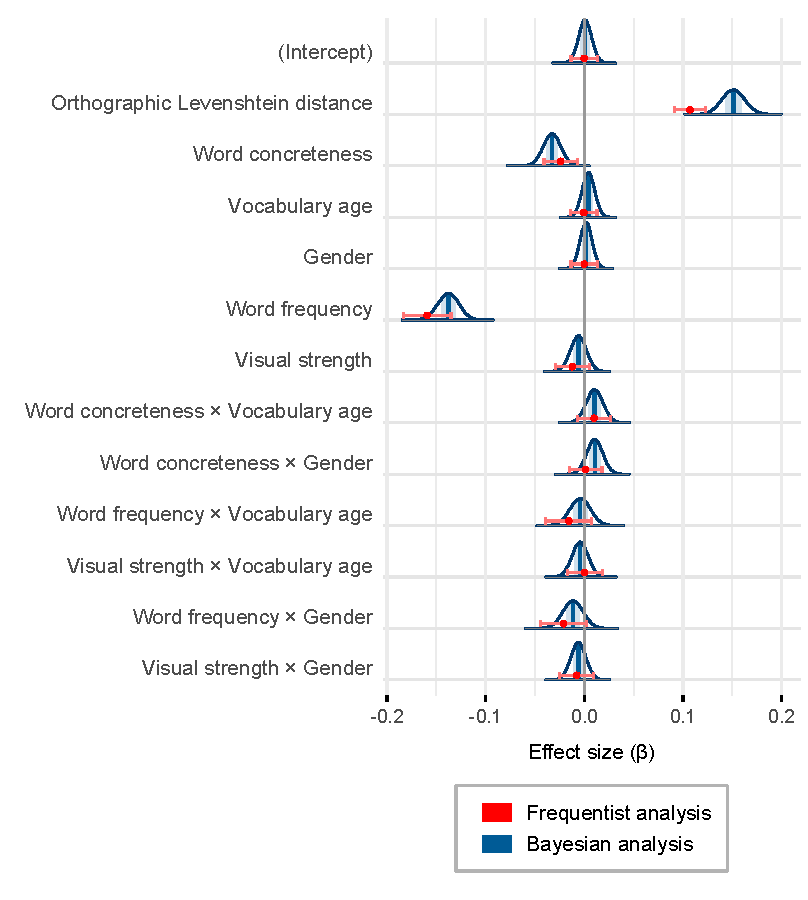
\includegraphics[width=1\linewidth]{/Users/pablodejuanbernabeu/Library/CloudStorage/OneDrive-LancasterUniversity/semanticpriming-semanticdecision-lexicaldecision/lexicaldecision/frequentist_bayesian_plots/plots/lexicaldecision_frequentist_bayesian_plot_weaklyinformativepriors_exgaussian} 

}

\caption{Estimates from the frequentist analysis (in red) and from the Bayesian analysis (in blue) for the lexical decision study. The frequentist means (represented by points) are flanked by 95\% confidence intervals. The Bayesian means (represented by vertical lines) are flanked by 95\% credible intervals, in light blue (in some cases, the interval is covered up by the bar of the mean).}\label{fig:lexicaldecision-frequentist-bayesian-plot-weaklyinformativepriors-exgaussian}
\end{figure}

\hypertarget{statistical-power-analysis-2}{%
\subsubsection{Statistical power analysis}\label{statistical-power-analysis-2}}

Figures \ref{fig:lexicaldecision-powercurve-plots-1-2-3} and \ref{fig:lexicaldecision-powercurve-plots-4-5-6-7} show the estimated power available for main effects and interactions of interest, respectively.

\begin{figure}

{\centering 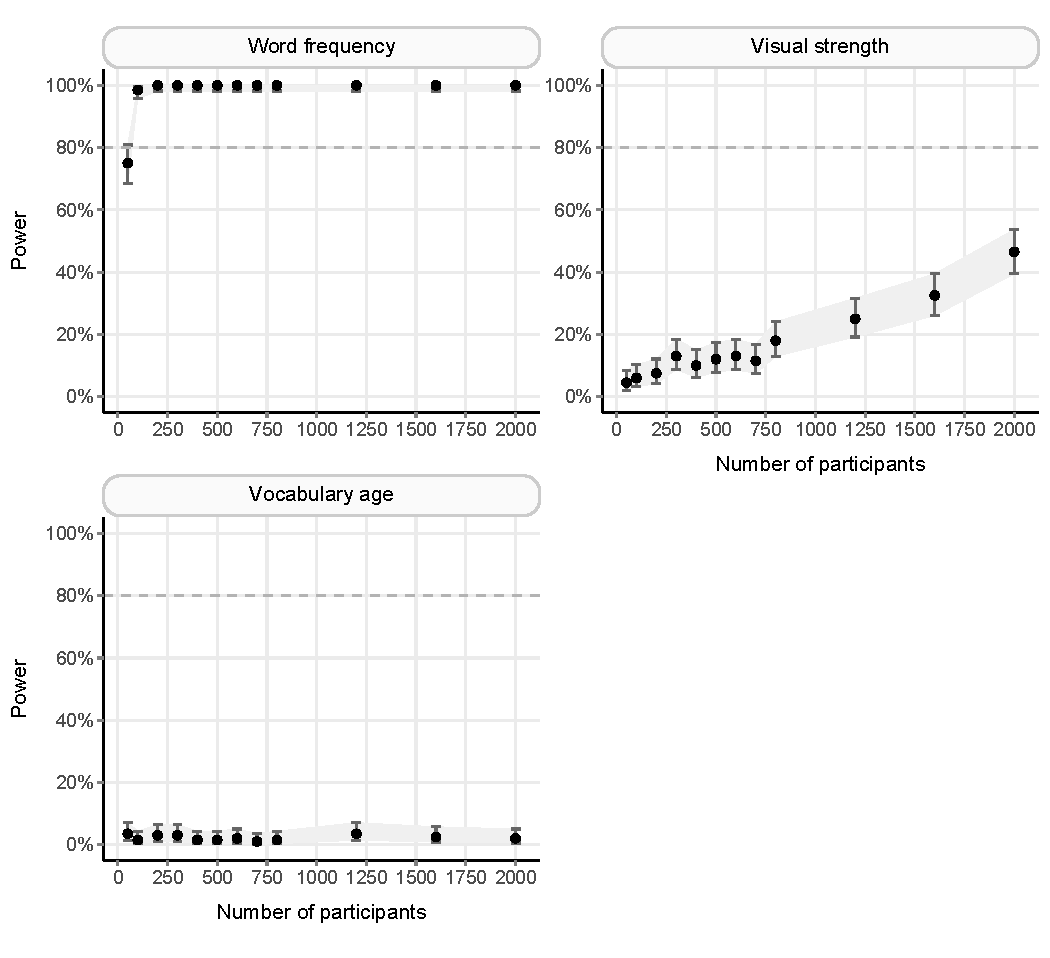
\includegraphics[width=1\linewidth]{/Users/pablodejuanbernabeu/Library/CloudStorage/OneDrive-LancasterUniversity/semanticpriming-semanticdecision-lexicaldecision/lexicaldecision/power_analysis/plots/lexicaldecision_powercurve_plots_1_2_3} 

}

\caption{Power curves for some main effects in the lexical decision study.}\label{fig:lexicaldecision-powercurve-plots-1-2-3}
\end{figure}

\begin{figure}

{\centering 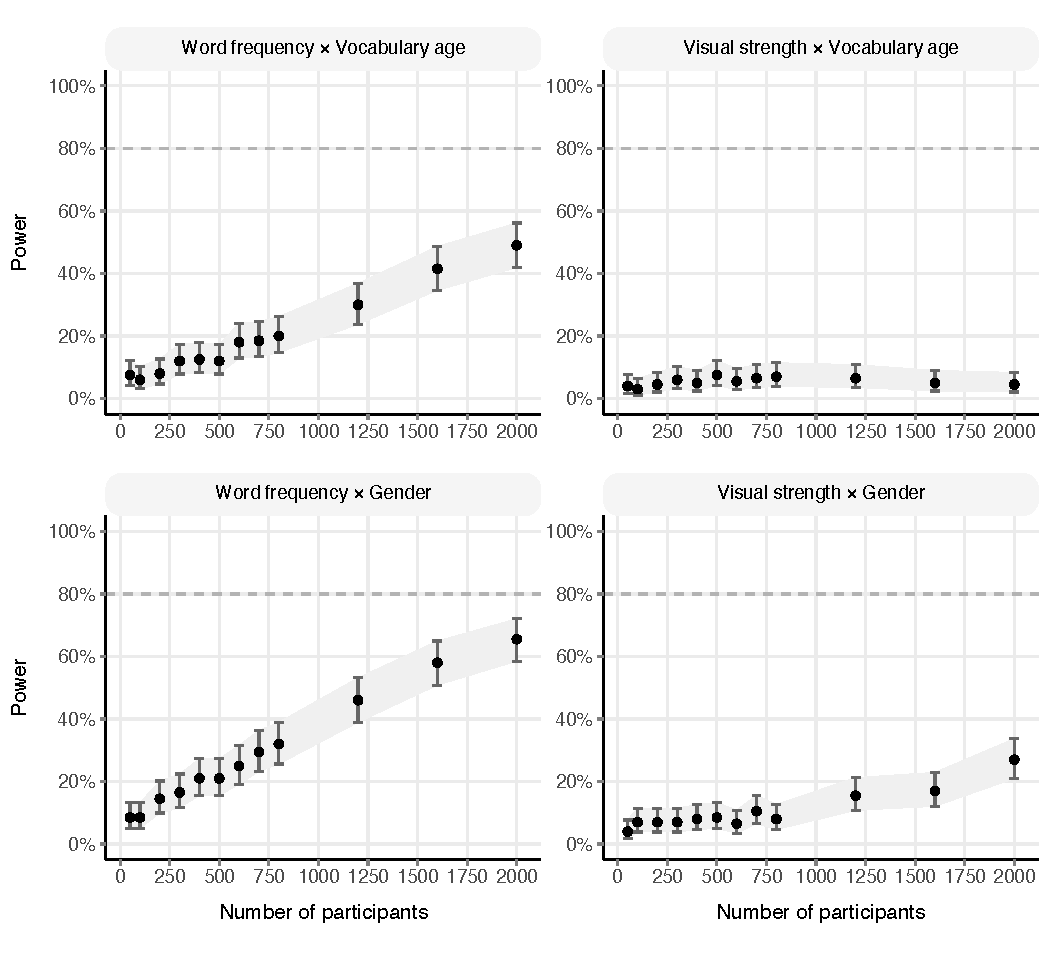
\includegraphics[width=1\linewidth]{/Users/pablodejuanbernabeu/Library/CloudStorage/OneDrive-LancasterUniversity/semanticpriming-semanticdecision-lexicaldecision/lexicaldecision/power_analysis/plots/lexicaldecision_powercurve_plots_4_5_6_7} 

}

\caption{Power curves for some interactions in the lexical decision study.}\label{fig:lexicaldecision-powercurve-plots-4-5-6-7}
\end{figure}

\_\_\_\_\_\_\_ interpret \_\_\_\_\_\_\_\_\_\_\_\_

\hypertarget{discussion-2}{%
\subsection{Discussion}\label{discussion-2}}

\begin{center}\rule{0.5\linewidth}{0.5pt}\end{center}

\hypertarget{general-discussion}{%
\section{General discussion}\label{general-discussion}}

In all three studies, the main effects and the interactions of language-based information were larger than those of vision-based information, consistent with previous research {[}\ldots{]}. Beyond that, the results revealed a dynamic process influenced by three levels of variation: participants, words and tasks. The associations that appeared across these levels revealed the roles of language-based and vision-based mechanisms in conceptual processing.

The RTs of higher-vocabulary participants were influenced by a smaller number of variables than those of lower-vocabulary participants. This converges with previous findings suggesting that higher and lower-vocabulary participants are affected by different variables. Potentially, the variables affecting higher-vocabulary participants are more relevant to the task (Lim et al., 2020; Pexman \& Yap, 2018; Yap et al., 2012, 2017).

\hypertarget{differences-between-measurement-instruments-and-the-associated-risks}{%
\subsection{Differences between measurement instruments and the associated risks}\label{differences-between-measurement-instruments-and-the-associated-risks}}

We also compared two measures of visual priming. The first measure was operationalised as the difference in visual strength (Lynott et al., 2020) between the prime and the target word in each trial. The second measure, created by (Petilli et al., 2021), was based on vector representations trained on images. The results revealed that the visual strength measure was significantly superior in explaining RTs. This difference was not due to an excessive collinearity between these measures (\(r\) = .02). Also importantly, both measures appeared to be valid based on their correlations with language-based similarity and with word concreteness.

If we indeed accept that both the above measures were valid, we must reflect on the possibility that measurement instruments create confounds when different systems are compared. That is, in the case of linguistic and embodied processing, the large difference between the effect sizes of these systems---found in the three current studies and in the previous literature {[}\ldots{]}---would not be trustworthy if the instruments that were used to measure the language system were far more precise than the instruments used to measure the embodiment system. In this sense, consider how variables are refined in research: it is done by comparing the performance of different variables. Critically, the literature seems to contain many comparisons of text-based variables, some dating from the 1990s (De Deyne et al., 2016, 2013; Günther et al., 2016a, 2016b; Jones et al., 2006; Lund \& Burgess, 1996; Mikolov et al., 2013; Wingfield \& Connell, 2022). In contrast, the work on embodiment variables began more than a decade afterwards, and this work has been more concerned with comparisons of different \emph{modalities}---e.g., valence, visual strength, auditory strength, etc. (Lynott et al., 2020; Lynott \& Connell, 2009; Newcombe et al., 2012). Thus, this historical discrepancy might in part (only in part) account for the superiority of linguistic information over embodied information, as found in the present study and in previous studies (Banks et al., 2021; Kiela \& Bottou, 2014; Lam et al., 2015; Louwerse et al., 2015; Pecher et al., 1998; Petilli et al., 2021).

The case of different measurement instruments is one of several factors that can exert a great influence in analyses. In the medium term, it may pay dividends to devote more work to comparing different instruments and, more generally, different analyses (see Barsalou, 2019; Botvinik-Nezer et al., 2020; Wagenmakers et al., 2022).

\hypertarget{statistical-power}{%
\subsection{Statistical power}\label{statistical-power}}

Power analyses were performed to \_\_\_\_\_\_\_\_\_\_\_\_\_\_\_\_\_\_\_\_\_. \_\_\_\_\_\_\_\_\_\_\_\_\_\_\_\_\_\_\_\_\_\_\_. The sample sizes required for some of the effects are not easily feasible with the usual distribution of funding in psychological research projects.

\clearpage

\hypertarget{references}{%
\section{References}\label{references}}

\hypertarget{refs}{}
\begin{CSLReferences}{1}{0}
\leavevmode\vadjust pre{\hypertarget{ref-albersWhenPowerAnalyses2018}{}}%
Albers, C., \& Lakens, D. (2018). When power analyses based on pilot data are biased: {Inaccurate} effect size estimators and follow-up bias. \emph{Journal of Experimental Social Psychology}, \emph{74}, 187--195. \url{https://doi.org/10.1016/j.jesp.2017.09.004}

\leavevmode\vadjust pre{\hypertarget{ref-amselTrackingRealtimeNeural2011}{}}%
Amsel, B. D. (2011). Tracking real-time neural activation of conceptual knowledge using single-trial event-related potentials. \emph{Neuropsychologia}, \emph{49}(5), 970--983. \url{https://doi.org/10.1016/j.neuropsychologia.2011.01.003}

\leavevmode\vadjust pre{\hypertarget{ref-amselEmpiricallyGroundingGrounded2014}{}}%
Amsel, B. D., Urbach, T. P., \& Kutas, M. (2014). Empirically grounding grounded cognition: {The} case of color. \emph{NeuroImage}, \emph{99}, 149--157. \url{https://doi.org/10.1016/j.neuroimage.2014.05.025}

\leavevmode\vadjust pre{\hypertarget{ref-andersonResponseCommentEstimating2016}{}}%
Anderson, C. J., Bahník, Š., Barnett-Cowan, M., Bosco, F. A., Chandler, J., Chartier, C. R., Cheung, F., Christopherson, C. D., Cordes, A., Cremata, E. J., Della Penna, N., Estel, V., Fedor, A., Fitneva, S. A., Frank, M. C., Grange, J. A., Hartshorne, J. K., Hasselman, F., Henninger, F., \ldots{} Zuni, K. (2016). Response to {Comment} on {``{Estimating} the reproducibility of psychological science.''} \emph{Science}, \emph{351}(6277), 1037--1037. \url{https://doi.org/10.1126/science.aad9163}

\leavevmode\vadjust pre{\hypertarget{ref-andrewsIntegratingExperientialDistributional2009}{}}%
Andrews, M., Vigliocco, G., \& Vinson, D. (2009). Integrating experiential and distributional data to learn semantic representations. \emph{Psychological Review}, \emph{116}(3), 463--498. \url{https://doi.org/10.1037/a0016261}

\leavevmode\vadjust pre{\hypertarget{ref-aujlaLanguageExperiencePredicts2021}{}}%
Aujla, H. (2021). Language experience predicts semantic priming of lexical decision. \emph{Canadian Journal of Experimental Psychology/Revue Canadienne de Psychologie Expérimentale}, \emph{75}(3), 235. \url{https://doi.org/10.1037/cep0000255}

\leavevmode\vadjust pre{\hypertarget{ref-balotaDepthAutomaticSpreading1986}{}}%
Balota, D. A., \& Lorch, R. F. (1986). Depth of automatic spreading activation: {Mediated} priming effects in pronunciation but not in lexical decision. \emph{Journal of Experimental Psychology: Learning, Memory, and Cognition}, \emph{12}(3), 336--345. \url{https://doi.org/10.1037/0278-7393.12.3.336}

\leavevmode\vadjust pre{\hypertarget{ref-balotaMeanResponseLatency2008}{}}%
Balota, D. A., Yap, M. J., Cortese, M. J., \& Watson, J. M. (2008). Beyond mean response latency: {Response} time distributional analyses of semantic priming. \emph{Journal of Memory and Language}, \emph{59}(4), 495--523. \url{https://doi.org/10.1016/j.jml.2007.10.004}

\leavevmode\vadjust pre{\hypertarget{ref-balota2007a}{}}%
Balota, D. A., Yap, M. J., Hutchison, K. A., Cortese, M. J., Kessler, B., Loftis, B., Neely, J. H., Nelson, D. L., Simpson, G. B., \& Treiman, R. (2007). The {English Lexicon Project}. \emph{Behavior Research Methods}, \emph{39}, 445--459. \url{https://doi.org/10.3758/BF03193014}

\leavevmode\vadjust pre{\hypertarget{ref-banksLinguisticDistributionalKnowledge2021}{}}%
Banks, B., Wingfield, C., \& Connell, L. (2021). Linguistic distributional knowledge and sensorimotor grounding both contribute to semantic category production. \emph{Cognitive Science}, \emph{45}(10), e13055. \url{https://doi.org/10.1111/cogs.13055}

\leavevmode\vadjust pre{\hypertarget{ref-barca2020a}{}}%
Barca, L., Mazzuca, C., \& Borghi, A. (2020). Overusing the pacifier during infancy sets a footprint on abstract words processing. \emph{Journal of Child Language}, \emph{47}(5), 1084--1099. \url{https://doi.org/10.1017/S0305000920000070}

\leavevmode\vadjust pre{\hypertarget{ref-barrRandomEffectsStructure2013}{}}%
Barr, D. J., Levy, R., Scheepers, C., \& Tily, H. J. (2013). Random effects structure for confirmatory hypothesis testing: {Keep} it maximal. \emph{Journal of Memory and Language}, \emph{68}(3), 255--278. \url{https://doi.org/10.1016/j.jml.2012.11.001}

\leavevmode\vadjust pre{\hypertarget{ref-barsalouEstablishingGeneralizableMechanisms2019}{}}%
Barsalou, L. W. (2019). Establishing generalizable mechanisms. \emph{Psychological Inquiry}, \emph{30}(4), 220--230. \url{https://doi.org/10.1080/1047840X.2019.1693857}

\leavevmode\vadjust pre{\hypertarget{ref-barsalouPerceptualSymbolSystems1999}{}}%
Barsalou, L. W. (1999). Perceptual symbol systems. \emph{Behavioral and Brain Sciences}, \emph{22}(4), 577--660. \url{https://doi.org/10.1017/S0140525X99002149}

\leavevmode\vadjust pre{\hypertarget{ref-barsalouLanguageSimulationConceptual2008}{}}%
Barsalou, L. W., Santos, A., Simmons, W. K., \& Wilson, C. D. (2008). Language and simulation in conceptual processing. In \emph{Symbols and {Embodiment}}. {Oxford University Press}. \url{https://doi.org/10.1093/acprof:oso/9780199217274.003.0013}

\leavevmode\vadjust pre{\hypertarget{ref-bartonWordlengthEffectReading2014}{}}%
Barton, J. J. S., Hanif, H. M., Eklinder Björnström, L., \& Hills, C. (2014). The word-length effect in reading: {A} review. \emph{Cognitive Neuropsychology}, \emph{31}(5-6), 378--412. \url{https://doi.org/10.1080/02643294.2014.895314}

\leavevmode\vadjust pre{\hypertarget{ref-batesFittingLinearMixedeffects2015}{}}%
Bates, D., Mächler, M., Bolker, B., \& Walker, S. (2015). Fitting linear mixed-effects models using {lme4}. \emph{Journal of Statistical Software}, \emph{67}, 1--48. \url{https://doi.org/10.18637/jss.v067.i01}

\leavevmode\vadjust pre{\hypertarget{ref-batesPackageLme42021}{}}%
Bates, D., Maechler, M., Bolker, B., Walker, S., Christensen, R. H. B., Singmann, H., Dai, B., Scheipl, F., Grothendieck, G., Green, P., Fox, J., Brauer, A., \& Krivitsky, P. N. (2021). \emph{Package '{lme4}'}. {CRAN}. \url{https://cran.r-project.org/web/packages/lme4/lme4.pdf}

\leavevmode\vadjust pre{\hypertarget{ref-beckerLongtermSemanticPriming1997}{}}%
Becker, S., Moscovitch, M., Behrmann, M., \& Joordens, S. (1997). Long-term semantic priming: {A} computational account and empirical evidence. \emph{Journal of Experimental Psychology: Learning, Memory, and Cognition}, \emph{23}(5), 1059--1082. \url{https://doi.org/10.1037/0278-7393.23.5.1059}

\leavevmode\vadjust pre{\hypertarget{ref-bernabeu2021a}{}}%
Bernabeu, P., Lynott, D., \& Connell, L. (2021). \emph{Preregistration: {The} interplay between linguistic and embodied systems in conceptual processing}. {OSF}. \url{https://osf.io/ftydw/}

\leavevmode\vadjust pre{\hypertarget{ref-bernabeu2017a}{}}%
Bernabeu, P., Willems, R. M., \& Louwerse, M. M. (2017). Modality switch effects emerge early and increase throughout conceptual processing: {Evidence} from {ERPs}. In G. Gunzelmann, A. Howes, T. Tenbrink, \& E. J. Davelaar (Eds.), \emph{Proceedings of the 39th {Annual Conference} of the {Cognitive Science Society}} (pp. 1629--1634). {Cognitive Science Society}. \url{https://mindmodeling.org/cogsci2017/papers/0318}

\leavevmode\vadjust pre{\hypertarget{ref-beyersmannEvidenceEmbeddedWord2020}{}}%
Beyersmann, E., Grainger, J., \& Taft, M. (2020). Evidence for embedded word length effects in complex nonwords. \emph{Language, Cognition and Neuroscience}, \emph{35}(2), 235--245. \url{https://doi.org/10.1080/23273798.2019.1659989}

\leavevmode\vadjust pre{\hypertarget{ref-borghiWordsSocialTools2019}{}}%
Borghi, A. M., Barca, L., Binkofski, F., Castelfranchi, C., Pezzulo, G., \& Tummolini, L. (2019). Words as social tools: {Language}, sociality and inner grounding in abstract concepts. \emph{Physics of Life Reviews}, \emph{29}, 120--153. \url{https://doi.org/10.1016/j.plrev.2018.12.001}

\leavevmode\vadjust pre{\hypertarget{ref-bottiniConcretenessAdvantageLexical2021}{}}%
Bottini, R., Morucci, P., D'Urso, A., Collignon, O., \& Crepaldi, D. (2021). The concreteness advantage in lexical decision does not depend on perceptual simulations. \emph{Journal of Experimental Psychology: General}. \url{https://doi.org/10.1037/xge0001090}

\leavevmode\vadjust pre{\hypertarget{ref-botvinik-nezerVariabilityAnalysisSingle2020}{}}%
Botvinik-Nezer, R., Holzmeister, F., Camerer, C. F., Dreber, A., Huber, J., Johannesson, M., Kirchler, M., Iwanir, R., Mumford, J. A., Adcock, R. A., Avesani, P., Baczkowski, B. M., Bajracharya, A., Bakst, L., Ball, S., Barilari, M., Bault, N., Beaton, D., Beitner, J., \ldots{} Schonberg, T. (2020). Variability in the analysis of a single neuroimaging dataset by many teams. \emph{Nature}, \emph{582}(7810, 7810), 84--88. \url{https://doi.org/10.1038/s41586-020-2314-9}

\leavevmode\vadjust pre{\hypertarget{ref-brauer2018a}{}}%
Brauer, M., \& Curtin, J. J. (2018). Linear mixed-effects models and the analysis of nonindependent data: {A} unified framework to analyze categorical and continuous independent variables that vary within-subjects and/or within-items. \emph{Psychological Methods}, \emph{23}(3), 389--411. \url{https://doi.org/10.1037/met0000159}

\leavevmode\vadjust pre{\hypertarget{ref-brysbaertHowManyParticipants2019}{}}%
Brysbaert, M. (2019). How many participants do we have to include in properly powered experiments? {A} tutorial of power analysis with reference tables. \emph{Journal of Cognition}, \emph{2}(1, 1), 16. \url{https://doi.org/10.5334/joc.72}

\leavevmode\vadjust pre{\hypertarget{ref-brysbaertWordRecognitionII2022}{}}%
Brysbaert, M. (2022). Word recognition {II}. In M. J. Snowling, C. Hulme, \& K. Nation, \emph{The science of reading} (pp. 79--101). {John Wiley \& Sons, Ltd}. \url{https://doi.org/10.1002/9781119705116.ch4}

\leavevmode\vadjust pre{\hypertarget{ref-brysbaertWordFrequencyEffect2018a}{}}%
Brysbaert, M., Mandera, P., \& Keuleers, E. (2018). The word frequency effect in word processing: {An} updated review. \emph{Current Directions in Psychological Science}, \emph{27}(1), 45--50. \url{https://doi.org/10.1177/0963721417727521}

\leavevmode\vadjust pre{\hypertarget{ref-brysbaertPowerAnalysisEffect2018}{}}%
Brysbaert, M., \& Stevens, M. (2018). Power analysis and effect size in mixed effects models: A tutorial. \emph{Journal of Cognition}, \emph{1}(1), 9. \url{https://doi.org/10.5334/joc.10}

\leavevmode\vadjust pre{\hypertarget{ref-brysbaertImpactWordPrevalence2016}{}}%
Brysbaert, M., Stevens, M., Mandera, P., \& Keuleers, E. (2016). The impact of word prevalence on lexical decision times: {Evidence} from the {Dutch Lexicon Project} 2. \emph{Journal of Experimental Psychology: Human Perception and Performance}, \emph{42}(3), 441--458. \url{https://doi.org/10.1037/xhp0000159}

\leavevmode\vadjust pre{\hypertarget{ref-brysbaert2014a}{}}%
Brysbaert, M., Warriner, A. B., \& Kuperman, V. (2014). Concreteness ratings for 40 thousand generally known {English} word lemmas. \emph{Behavior Research Methods}, \emph{46}, 904--911. \url{https://doi.org/10.3758/s13428-013-0403-5}

\leavevmode\vadjust pre{\hypertarget{ref-bullinariaExtractingSemanticRepresentations2007}{}}%
Bullinaria, J. A., \& Levy, J. P. (2007). Extracting semantic representations from word co-occurrence statistics: {A} computational study. \emph{Behavior Research Methods}, \emph{39}(3), 510--526. \url{https://doi.org/10.3758/BF03193020}

\leavevmode\vadjust pre{\hypertarget{ref-burknerAdvancedBayesianMultilevel2018}{}}%
Bürkner, P.-C. (2018). Advanced {Bayesian} multilevel modeling with the {R} package {brms}. \emph{The R Journal}, \emph{10}(1), 395--411. \url{https://journal.r-project.org/archive/2018/RJ-2018-017/index.html}

\leavevmode\vadjust pre{\hypertarget{ref-burknerPackageBrms2022}{}}%
Bürkner, P.-C., Gabry, J., Weber, S., Johnson, A., Modrak, M., Badr, H. S., Weber, F., Ben-Shachar, M. S., \& Rabel, H. (2022). \emph{Package '{brms}'}. {CRAN}. \url{https://cran.r-project.org/web/packages/brms/brms.pdf}

\leavevmode\vadjust pre{\hypertarget{ref-burman2008a}{}}%
Burman, D., Bitan, T., \& Both, J. (2008). Sex differences in neural processing of language among children. \emph{Neuropsychologia}, \emph{46, 5}, 1349--1362. \url{https://doi.org/10.1016/j.neuropsychologia.2007.12.021}

\leavevmode\vadjust pre{\hypertarget{ref-buttonPowerFailureWhy2013}{}}%
Button, K. S., Ioannidis, J. P. A., Mokrysz, C., Nosek, B. A., Flint, J., Robinson, E. S. J., \& Munafò, M. R. (2013). Power failure: {Why} small sample size undermines the reliability of neuroscience. \emph{Nature Reviews Neuroscience}, \emph{14}(5, 5), 365--376. \url{https://doi.org/10.1038/nrn3475}

\leavevmode\vadjust pre{\hypertarget{ref-cerniMotorExpertiseTyping2016}{}}%
Cerni, T., Velay, J.-L., Alario, F.-X., Vaugoyeau, M., \& Longcamp, M. (2016). Motor expertise for typing impacts lexical decision performance. \emph{Trends in Neuroscience and Education}, \emph{5}(3), 130--138. \url{https://doi.org/10.1016/j.tine.2016.07.007}

\leavevmode\vadjust pre{\hypertarget{ref-charbonnierPredictingConcretenessGerman2020}{}}%
Charbonnier, J., \& Wartena, C. (2020). Predicting the concreteness of {German} words. \emph{Proceedings of the 5th {Swiss Text Analytics Conference} ({SwissText})}, \emph{2624}. \url{https://doi.org/10.25968/opus-2075}

\leavevmode\vadjust pre{\hypertarget{ref-charbonnierPredictingWordConcreteness2019}{}}%
Charbonnier, J., \& Wartena, C. (2019). Predicting word concreteness and imagery. \emph{Proceedings of the 13th {International Conference} on {Computational Semantics} - {Long Papers}}, 176--187. \url{https://doi.org/10.18653/v1/W19-0415}

\leavevmode\vadjust pre{\hypertarget{ref-cohenCostDichotomization1983}{}}%
Cohen, J. (1983). The cost of dichotomization. \emph{Applied Psychological Measurement}, \emph{7}(3), 249--253. \url{https://doi.org/10.1177/014662168300700301}

\leavevmode\vadjust pre{\hypertarget{ref-collinsModalitySwitchingProperty2011}{}}%
Collins, J., Pecher, D., Zeelenberg, R., \& Coulson, S. (2011). Modality switching in a property verification task: {An} erp study of what happens when candles flicker after high heels click. \emph{Frontiers in Psychology}, \emph{2}. \url{https://www.frontiersin.org/article/10.3389/fpsyg.2011.00010}

\leavevmode\vadjust pre{\hypertarget{ref-concaSearchDifferentCategories2021}{}}%
Conca, F., Catricalà, E., Canini, M., Petrini, A., Vigliocco, G., Cappa, S. F., \& Della Rosa, P. A. (2021). In search of different categories of abstract concepts: A {fMRI} adaptation study. \emph{Scientific Reports}, \emph{11}(1, 1), 22587. \url{https://doi.org/10.1038/s41598-021-02013-8}

\leavevmode\vadjust pre{\hypertarget{ref-connell2019a}{}}%
Connell, L. (2019). What have labels ever done for us? {The} linguistic shortcut in conceptual processing. \emph{Language, Cognition and Neuroscience}, \emph{34}(10), 1308--1318. \url{https://doi.org/10.1080/23273798.2018.1471512}

\leavevmode\vadjust pre{\hypertarget{ref-connellStrengthPerceptualExperience2012}{}}%
Connell, L., \& Lynott, D. (2012). Strength of perceptual experience predicts word processing performance better than concreteness or imageability. \emph{Cognition}, \emph{125}(3), 452--465. \url{https://doi.org/10.1016/j.cognition.2012.07.010}

\leavevmode\vadjust pre{\hypertarget{ref-connell2013a}{}}%
Connell, L., \& Lynott, D. (2013). Flexible and fast: {Linguistic} shortcut affects both shallow and deep conceptual processing. \emph{Psychonomic Bulletin \& Review}, \emph{20, 3}, 542--550. \url{https://doi.org/10.3758/s13423-012-0368-x}

\leavevmode\vadjust pre{\hypertarget{ref-connellSeeHearWhat2014}{}}%
Connell, L., \& Lynott, D. (2014). I see/hear what you mean: {Semantic} activation in visual word recognition depends on perceptual attention. \emph{Journal of Experimental Psychology: General}, \emph{143}(2), 527--533. \url{https://doi.org/10.1037/a0034626}

\leavevmode\vadjust pre{\hypertarget{ref-connellWeKnowWhat2016}{}}%
Connell, L., \& Lynott, D. (2016). Do we know what we're simulating? {Information} loss on transferring unconscious perceptual simulation to conscious imagery. \emph{Journal of Experimental Psychology: Learning, Memory, and Cognition}, \emph{42}(8), 1218--1232. \url{https://doi.org/10.1037/xlm0000245}

\leavevmode\vadjust pre{\hypertarget{ref-connellInteroceptionForgottenModality2018}{}}%
Connell, L., Lynott, D., \& Banks, B. (2018). Interoception: The forgotten modality in perceptual grounding of abstract and concrete concepts. \emph{Philosophical Transactions of the Royal Society B: Biological Sciences}, \emph{373}(1752), 20170143. \url{https://doi.org/10.1098/rstb.2017.0143}

\leavevmode\vadjust pre{\hypertarget{ref-contreraskallensQuantifyingInterdisciplinarityCognitive2022}{}}%
Contreras Kallens, P., Dale, R., \& Christiansen, M. H. (2022). Quantifying interdisciplinarity in cognitive science and beyond. \emph{Topics in Cognitive Science}. \url{https://doi.org/10.1111/tops.12609}

\leavevmode\vadjust pre{\hypertarget{ref-corkerHighQualityDirect2014}{}}%
Corker, K. S., Lynott, D., Wortman, J., Connell, L., Donnellan, M. B., Lucas, R. E., \& O'Brien, K. (2014). High quality direct replications matter: {Response} to {Williams} (2014). \emph{Social Psychology}, \emph{45}(4), 324--326.

\leavevmode\vadjust pre{\hypertarget{ref-cummingNewStatisticsWhy2014}{}}%
Cumming, G. (2014). The new statistics: {Why} and how. \emph{Psychological Science}, \emph{25}(1), 7--29. \url{https://doi.org/10.1177/0956797613504966}

\leavevmode\vadjust pre{\hypertarget{ref-davies2017a}{}}%
Davies, R. A., Arnell, R., Birchenough, J. M., Grimmond, D., \& Houlson, S. (2017). Reading through the life span: {Individual} differences in psycholinguistic effects. \emph{Journal of Experimental Psychology: Learning, Memory, and Cognition}, \emph{43}(8), 1298. \url{https://doi.org/10.1037/xlm0000366}

\leavevmode\vadjust pre{\hypertarget{ref-dedeyneVisualAffectiveMultimodal2021}{}}%
De Deyne, S., Navarro, D. J., Collell, G., \& Perfors, A. (2021). Visual and affective multimodal models of word meaning in language and mind. \emph{Cognitive Science}, \emph{45}(1), e12922. \url{https://doi.org/10.1111/cogs.12922}

\leavevmode\vadjust pre{\hypertarget{ref-de2019a}{}}%
De Deyne, S., Navarro, D. J., Perfors, A., Brysbaert, M., \& Storms, G. (2019). The {``{Small World} of {Words}''} {English} word association norms for over 12,000 cue words. \emph{Behavior Research Methods}, \emph{51}, 987--1006. \url{https://doi.org/10.3758/s13428-018-1115-7}

\leavevmode\vadjust pre{\hypertarget{ref-dedeyneBetterExplanationsLexical2013}{}}%
De Deyne, S., Navarro, D. J., \& Storms, G. (2013). Better explanations of lexical and semantic cognition using networks derived from continued rather than single-word associations. \emph{Behavior Research Methods}, \emph{45}(2), 480--498. \url{https://doi.org/10.3758/s13428-012-0260-7}

\leavevmode\vadjust pre{\hypertarget{ref-de2016a}{}}%
De Deyne, S., Perfors, A., \& Navarro, D. (2016). Predicting human similarity judgments with distributional models: {The} value of word associations. \emph{Proceedings of {COLING} 2016, the 26th International Conference on Computational Linguistics: {Technical} Papers}, 1861--1870.

\leavevmode\vadjust pre{\hypertarget{ref-dewitMaskedSemanticPriming2015}{}}%
de Wit, B., \& Kinoshita, S. (2015). The masked semantic priming effect is task dependent: {Reconsidering} the automatic spreading activation process. \emph{Journal of Experimental Psychology: Learning, Memory, and Cognition}, \emph{41}(4), 1062--1075. \url{https://doi.org/10.1037/xlm0000074}

\leavevmode\vadjust pre{\hypertarget{ref-dilolloDecouplingStimulusDuration2004}{}}%
Di Lollo, V., Mühlenen, A. von, Enns, J. T., \& Bridgeman, B. (2004). Decoupling stimulus duration from brightness in metacontrast masking: {Data} and models. \emph{Journal of Experimental Psychology: Human Perception and Performance}, \emph{30}(4), 733--745. \url{https://doi.org/10.1037/0096-1523.30.4.733}

\leavevmode\vadjust pre{\hypertarget{ref-diazNeuralSensitivityPhonological2021}{}}%
Diaz, M. T., Karimi, H., Troutman, S. B. W., Gertel, V. H., Cosgrove, A. L., \& Zhang, H. (2021). Neural sensitivity to phonological characteristics is stable across the lifespan. \emph{NeuroImage}, \emph{225}, 117511. \url{https://doi.org/10.1016/j.neuroimage.2020.117511}

\leavevmode\vadjust pre{\hypertarget{ref-dijkstraMultilinkComputationalModel2019}{}}%
Dijkstra, T., Wahl, A., Buytenhuijs, F., Halem, N. V., Al-Jibouri, Z., Korte, M. D., \& Rekké, S. (2019). Multilink: {A} computational model for bilingual word recognition and word translation. \emph{Bilingualism: Language and Cognition}, \emph{22}(4), 657--679. \url{https://doi.org/10.1017/S1366728918000287}

\leavevmode\vadjust pre{\hypertarget{ref-dils2010a}{}}%
Dils, A. T., \& Boroditsky, L. (2010). Visual motion aftereffect from understanding motion language. \emph{Proceedings of the National Academy of Sciences}, \emph{107}(37), 16396--16400. \url{https://doi.org/10.1073/pnas.1009438107}

\leavevmode\vadjust pre{\hypertarget{ref-diveicaQuantifyingSocialSemantics2022}{}}%
Diveica, V., Pexman, P. M., \& Binney, R. J. (2022). Quantifying social semantics: {An} inclusive definition of socialness and ratings for 8388 {English} words. \emph{Behavior Research Methods}. \url{https://doi.org/10.3758/s13428-022-01810-x}

\leavevmode\vadjust pre{\hypertarget{ref-dormannCollinearityReviewMethods2013}{}}%
Dormann, C. F., Elith, J., Bacher, S., Buchmann, C., Carl, G., Carré, G., Marquéz, J. R. G., Gruber, B., Lafourcade, B., Leitão, P. J., Münkemüller, T., McClean, C., Osborne, P. E., Reineking, B., Schröder, B., Skidmore, A. K., Zurell, D., \& Lautenbach, S. (2013). Collinearity: A review of methods to deal with it and a simulation study evaluating their performance. \emph{Ecography}, \emph{36}(1), 27--46. \url{https://doi.org/10.1111/j.1600-0587.2012.07348.x}

\leavevmode\vadjust pre{\hypertarget{ref-dove2020a}{}}%
Dove, G. (2020). More than a scaffold: {Language} is a neuroenhancement. \emph{Cognitive Neuropsychology}, \emph{37}(5-6), 288--311. \url{https://doi.org/10.1080/02643294.2019.1637338}

\leavevmode\vadjust pre{\hypertarget{ref-dunabeitiaQualitativeDifferencesRepresentation2009}{}}%
Duñabeitia, J. A., Avilés, A., Afonso, O., Scheepers, C., \& Carreiras, M. (2009). Qualitative differences in the representation of abstract versus concrete words: {Evidence} from the visual-world paradigm. \emph{Cognition}, \emph{110}(2), 284--292. \url{https://doi.org/10.1016/j.cognition.2008.11.012}

\leavevmode\vadjust pre{\hypertarget{ref-faust1999a}{}}%
Faust, M. E., Balota, D. A., Spieler, D. H., \& Ferraro, F. R. (1999). Individual differences in information-processing rate and amount: {Implications} for group differences in response latency. \emph{Psychological Bulletin}, \emph{125}, 777--799. \url{https://doi.org/10.1037/0033-2909.125.6.777}

\leavevmode\vadjust pre{\hypertarget{ref-fernandinoDecodingInformationStructure2022}{}}%
Fernandino, L., Tong, J.-Q., Conant, L. L., Humphries, C. J., \& Binder, J. R. (2022). Decoding the information structure underlying the neural representation of concepts. \emph{Proceedings of the National Academy of Sciences}, \emph{119}(6). \url{https://doi.org/10.1073/pnas.2108091119}

\leavevmode\vadjust pre{\hypertarget{ref-fettermanFeelingWarmBeing2018}{}}%
Fetterman, A. K., Wilkowski, B. M., \& Robinson, M. D. (2018). On feeling warm and being warm: {Daily} perceptions of physical warmth fluctuate with interpersonal warmth. \emph{Social Psychological and Personality Science}, \emph{9}(5), 560--567. \url{https://doi.org/10.1177/1948550617712032}

\leavevmode\vadjust pre{\hypertarget{ref-fleurDefinitelySawIt2020}{}}%
Fleur, D. S., Flecken, M., Rommers, J., \& Nieuwland, M. S. (2020). Definitely saw it coming? {The} dual nature of the pre-nominal prediction effect. \emph{Cognition}, \emph{204}, 104335. \url{https://doi.org/10.1016/j.cognition.2020.104335}

\leavevmode\vadjust pre{\hypertarget{ref-floresdarcaisSemanticActivationRecognition1985}{}}%
Flores d'Arcais, G. B., Schreuder, R., \& Glazenborg, G. (1985). Semantic activation during recognition of referential words. \emph{Psychological Research}, \emph{47}(1), 39--49. \url{https://doi.org/10.1007/BF00309217}

\leavevmode\vadjust pre{\hypertarget{ref-foxGeneralizedLinearModels2016}{}}%
Fox, J. (2016). Generalized linear models. In \emph{Applied regression analysis and generalized linear models} (Third Edition, pp. 418--472). {SAGE}.

\leavevmode\vadjust pre{\hypertarget{ref-gagneProcessingEnglishCompounds2016}{}}%
Gagné, C. L., Spalding, T. L., \& Nisbet, K. A. (2016). Processing english compounds: {Investigating} semantic transparency. \emph{SKASE Journal of Theoretical Linguistics}, \emph{13}(2), 2--22. \url{https://link.gale.com/apps/doc/A469757337/LitRC?u=anon~b6a332f4\&xid=9960afc7}

\leavevmode\vadjust pre{\hypertarget{ref-galleseBrainConceptsRole2005}{}}%
Gallese, V., \& Lakoff, G. (2005). The {Brain}'s concepts: The role of the {Sensory-motor} system in conceptual knowledge. \emph{Cognitive Neuropsychology}, \emph{22}(3-4), 455--479. \url{https://doi.org/10.1080/02643290442000310}

\leavevmode\vadjust pre{\hypertarget{ref-garceaPreservedToolKnowledge2013}{}}%
Garcea, F., Dombovy, M., \& Mahon, B. Z. (2013). Preserved {Tool Knowledge} in the {Context} of {Impaired Action Knowledge}: {Implications} for {Models} of {Semantic Memory}. \emph{Frontiers in Human Neuroscience}, \emph{7}, 120. \url{https://doi.org/10.3389/fnhum.2013.00120}

\leavevmode\vadjust pre{\hypertarget{ref-garciaTimeFaceLanguage2020}{}}%
García, A. M., Hesse, E., Birba, A., Adolfi, F., Mikulan, E., Caro, M. M., Petroni, A., Bekinschtein, T. A., del Carmen García, M., Silva, W., Ciraolo, C., Vaucheret, E., Sedeño, L., \& Ibáñez, A. (2020). Time to face language: Embodied mechanisms underpin the inception of face-related meanings in the human brain. \emph{Cerebral Cortex}, \emph{30}(11), 6051--6068. \url{https://doi.org/10.1093/cercor/bhaa178}

\leavevmode\vadjust pre{\hypertarget{ref-gelmanPowerCalculationsAssessing2014}{}}%
Gelman, A., \& Carlin, J. (2014). Beyond power calculations: Assessing type s (sign) and type m (magnitude) errors. \emph{Perspectives on Psychological Science}, \emph{9}(6), 641--651. \url{https://doi.org/10.1177/1745691614551642}

\leavevmode\vadjust pre{\hypertarget{ref-gelmanPosteriorPredictiveAssessment1996}{}}%
Gelman, A., Meng, X., \& Stern, H. (1996). Posterior predictive assessment of model fitness via realized discrepancies. \emph{Statistica Sinica}, 733--807.

\leavevmode\vadjust pre{\hypertarget{ref-gilbertCommentEstimatingReproducibility2016}{}}%
Gilbert, D. T., King, G., Pettigrew, S., \& Wilson, T. D. (2016). Comment on {``{Estimating} the reproducibility of psychological science.''} \emph{Science}, \emph{351}(6277), 1037--1037. \url{https://doi.org/10.1126/science.aad7243}

\leavevmode\vadjust pre{\hypertarget{ref-greenSIMRPackagePower2016}{}}%
Green, P., \& MacLeod, C. J. (2016). {SIMR}: {An R} package for power analysis of generalized linear mixed models by simulation. \emph{Methods in Ecology and Evolution}, \emph{7}(4), 493--498. \url{https://doi.org/10.1111/2041-210X.12504}

\leavevmode\vadjust pre{\hypertarget{ref-guntherLatentSemanticAnalysis2016}{}}%
Günther, F., Dudschig, C., \& Kaup, B. (2016a). Latent semantic analysis cosines as a cognitive similarity measure: {Evidence} from priming studies. \emph{Quarterly Journal of Experimental Psychology}, \emph{69}(4), 626--653. \url{https://doi.org/10.1080/17470218.2015.1038280}

\leavevmode\vadjust pre{\hypertarget{ref-guenther2016a}{}}%
Günther, F., Dudschig, C., \& Kaup, B. (2016b). Predicting lexical priming effects from distributional semantic similarities: {A} replication with extension. \emph{Frontiers in Psychology}, \emph{7}. \url{https://doi.org/10.3389/fpsyg.2016.01646}

\leavevmode\vadjust pre{\hypertarget{ref-guntherSymbolGroundingDirect2018}{}}%
Günther, F., Dudschig, C., \& Kaup, B. (2018). Symbol grounding without direct experience: Do words inherit sensorimotor activation from purely linguistic context? \emph{Cognitive Science}, \emph{42}(S2), 336--374. \url{https://doi.org/10.1111/cogs.12549}

\leavevmode\vadjust pre{\hypertarget{ref-guntherLimitsAutomaticSensorimotor2021}{}}%
Günther, F., Press, S. A., Dudschig, C., \& Kaup, B. (2021). The limits of automatic sensorimotor processing during word processing: Investigations with repeated linguistic experience, memory consolidation during sleep, and rich linguistic learning contexts. \emph{Psychological Research}. \url{https://doi.org/10.1007/s00426-021-01620-4}

\leavevmode\vadjust pre{\hypertarget{ref-haldEEGThetaGamma2006}{}}%
Hald, L. A., Bastiaansen, M. C. M., \& Hagoort, P. (2006). {EEG} theta and gamma responses to semantic violations in online sentence processing. \emph{Brain and Language}, \emph{96}(1), 90--105. \url{https://doi.org/10.1016/j.bandl.2005.06.007}

\leavevmode\vadjust pre{\hypertarget{ref-hald2013a}{}}%
Hald, L. A., Hocking, I., Vernon, D., Marshall, J. A., \& Garnham, A. (2013). Exploring modality switching effects in negated sentences: {Further} evidence for grounded representations. \emph{Frontiers in Psychology}, \emph{4}, 93. \url{https://doi.org/10.3389/fpsyg.2013.00093}

\leavevmode\vadjust pre{\hypertarget{ref-hald2011a}{}}%
Hald, L. A., Marshall, J. A., Janssen, D. P., \& Garnham, A. (2011). Switching modalities in a sentence verification task: {ERP} evidence for embodied language processing. \emph{Frontiers in Psychology}, \emph{2}, 45. \url{https://doi.org/10.3389/fpsyg.2011.00045}

\leavevmode\vadjust pre{\hypertarget{ref-harnadSymbolGroundingProblem1990}{}}%
Harnad, S. (1990). The symbol grounding problem. \emph{Physica D: Nonlinear Phenomena}, \emph{42}(1), 335--346. \url{https://doi.org/10.1016/0167-2789(90)90087-6}

\leavevmode\vadjust pre{\hypertarget{ref-harrison2018a}{}}%
Harrison, X. A., Donaldson, L., Correa-Cano, M. E., Evans, J., Fisher, D. N., Goodwin, C., Robinson, B. S., Hodgson, D. J., \& Inger, R. (2018). A brief introduction to mixed effects modelling and multi-model inference in ecology. \emph{PeerJ}, \emph{6}, 4794. \url{https://doi.org/10.7717/peerj.4794}

\leavevmode\vadjust pre{\hypertarget{ref-haukOnlyTimeWill2016}{}}%
Hauk, O. (2016). Only time will tell -- why temporal information is essential for our neuroscientific understanding of semantics. \emph{Psychonomic Bulletin \& Review}, \emph{23}(4), 1072--1079. \url{https://doi.org/10.3758/s13423-015-0873-9}

\leavevmode\vadjust pre{\hypertarget{ref-hedge2018a}{}}%
Hedge, C., Powell, G., \& Sumner, P. (2018). The reliability paradox: {Why} robust cognitive tasks do not produce reliable individual differences. \emph{Behavior Research Methods}, \emph{50}(3), 1166--1186. \url{https://doi.org/10.3758/s13428-017-0935-1}

\leavevmode\vadjust pre{\hypertarget{ref-henrich2010a}{}}%
Henrich, J., Heine, S. J., \& Norenzayan, A. (2010). The weirdest people in the world? \emph{Behavioral and Brain Sciences}, \emph{33}(2-3), 61--135. \url{https://doi.org/10.1017/S0140525X0999152X}

\leavevmode\vadjust pre{\hypertarget{ref-hoedemakerItTakesTime2014}{}}%
Hoedemaker, R. S., \& Gordon, P. C. (2014). It takes time to prime: {Semantic} priming in the ocular lexical decision task. \emph{Journal of Experimental Psychology: Human Perception and Performance}, \emph{40}(6), 2179--2197. \url{https://doi.org/10.1037/a0037677}

\leavevmode\vadjust pre{\hypertarget{ref-hoenigAbusePower2001}{}}%
Hoenig, J. M., \& Heisey, D. M. (2001). The {Abuse} of {Power}. \emph{The American Statistician}, \emph{55}(1), 19--24. \url{https://doi.org/10.1198/000313001300339897}

\leavevmode\vadjust pre{\hypertarget{ref-holt2006a}{}}%
Holt, L. E., \& Beilock, S. L. (2006). Expertise and its embodiment: {Examining} the impact of sensorimotor skill expertise on the representation of action-related text. \emph{Psychonomic Bulletin \& Review}, \emph{13}(4), 694--701. \url{https://doi.org/10.3758/BF03193983}

\leavevmode\vadjust pre{\hypertarget{ref-hultenNeuralRepresentationAbstract2021}{}}%
Hultén, A., Vliet, M. van, Kivisaari, S., Lammi, L., Lindh-Knuutila, T., Faisal, A., \& Salmelin, R. (2021). The neural representation of abstract words may arise through grounding word meaning in language itself. \emph{Human Brain Mapping}, \emph{42}(15), 4973--4984. \url{https://onlinelibrary.wiley.com/doi/abs/10.1002/hbm.25593}

\leavevmode\vadjust pre{\hypertarget{ref-hutchinson2013a}{}}%
Hutchinson, S., \& Louwerse, M. M. (2013). Language statistics and individual differences in processing primary metaphors. \emph{Cognitive Linguistics}, \emph{24}(4), 667--687. \url{https://doi.org/10.1515/cog-2013-0023}

\leavevmode\vadjust pre{\hypertarget{ref-hutchisonSemanticPrimingDue2003}{}}%
Hutchison, K. A. (2003). Is semantic priming due to association strength or feature overlap? {A} microanalytic review. \emph{Psychonomic Bulletin \& Review}, \emph{10}(4), 785--813. \url{https://doi.org/10.3758/BF03196544}

\leavevmode\vadjust pre{\hypertarget{ref-hutchisonPredictingSemanticPriming2008}{}}%
Hutchison, K. A., Balota, D. A., Cortese, M. J., \& Watson, J. M. (2008). Predicting semantic priming at the item level. \emph{Quarterly Journal of Experimental Psychology}, \emph{61}(7), 1036--1066. \url{https://doi.org/10.1080/17470210701438111}

\leavevmode\vadjust pre{\hypertarget{ref-hutchison2013a}{}}%
Hutchison, K. A., Balota, D. A., Neely, J. H., Cortese, M. J., Cohen-Shikora, E. R., Tse, C.-S., Yap, M. J., Bengson, J. J., Niemeyer, D., \& Buchanan, E. (2013). The semantic priming project. \emph{Behavior Research Methods}, \emph{45}, 1099--1114. \url{https://doi.org/10.3758/s13428-012-0304-z}

\leavevmode\vadjust pre{\hypertarget{ref-james2018a}{}}%
James, A. N., Fraundorf, S. H., Lee, E. K., \& Watson, D. G. (2018). Individual differences in syntactic processing: {Is} there evidence for reader-text interactions? \emph{Journal of Memory and Language}, \emph{102}, 155--181. \url{https://doi.org/10.1016/j.jml.2018.05.006}

\leavevmode\vadjust pre{\hypertarget{ref-jones2006a}{}}%
Jones, M. N., Kintsch, W., \& Mewhort, D. J. (2006). High-dimensional semantic space accounts of priming. \emph{Journal of Memory and Language}, \emph{55}(4), 534--552. \url{https://doi.org/10.1016/j.jml.2006.07.003}

\leavevmode\vadjust pre{\hypertarget{ref-joordensLongShortSemantic1997}{}}%
Joordens, S., \& Becker, S. (1997). The long and short of semantic priming effects in lexical decision. \emph{Journal of Experimental Psychology: Learning, Memory, and Cognition}, \emph{23}(5), 1083--1105. \url{https://doi.org/10.1037/0278-7393.23.5.1083}

\leavevmode\vadjust pre{\hypertarget{ref-jung2019a}{}}%
Jung, M., Mody, M., Fujioka, T., Kimura, Y., Okazawa, H., \& Kosaka, H. (2019). Sex differences in white matter pathways related to language ability. \emph{Frontiers in Human Neuroscience}, \emph{13}, 898. \url{https://doi.org/10.3389/fnins.2019.00898}

\leavevmode\vadjust pre{\hypertarget{ref-kieferDifferentialTemporospatialPattern2022}{}}%
Kiefer, M., Pielke, L., \& Trumpp, N. M. (2022). Differential temporo-spatial pattern of electrical brain activity during the processing of abstract concepts related to mental states and verbal associations. \emph{NeuroImage}, \emph{252}, 119036. \url{https://doi.org/10.1016/j.neuroimage.2022.119036}

\leavevmode\vadjust pre{\hypertarget{ref-kiela2014a}{}}%
Kiela, D., \& Bottou, L. (2014). Learning image embeddings using convolutional neural networks for improved multi-modal semantics. \emph{Proceedings of the 2014 Conference on Empirical Methods in Natural Language Processing ({EMNLP}}, 36--45. \url{https://doi.org/10.3115/v1/D14-1005}

\leavevmode\vadjust pre{\hypertarget{ref-kimEffectsLexicalFeatures2018}{}}%
Kim, M., Crossley, S. A., \& Skalicky, S. (2018). Effects of lexical features, textual properties, and individual differences on word processing times during second language reading comprehension. \emph{Reading and Writing}, \emph{31}(5), 1155--1180. \url{https://doi.org/10.1007/s11145-018-9833-x}

\leavevmode\vadjust pre{\hypertarget{ref-kniefViolatingNormalityAssumption2021}{}}%
Knief, U., \& Forstmeier, W. (2021). Violating the normality assumption may be the lesser of two evils. \emph{Behavior Research Methods}. \url{https://doi.org/10.3758/s13428-021-01587-5}

\leavevmode\vadjust pre{\hypertarget{ref-R-robustlmm}{}}%
Koller, M. (2016). {robustlmm}: An {R} package for robust estimation of linear mixed-effects models. \emph{Journal of Statistical Software}, \emph{75}(6), 1--24. \url{https://doi.org/10.18637/jss.v075.i06}

\leavevmode\vadjust pre{\hypertarget{ref-kosIndividualVariationLate2012}{}}%
Kos, M., Van den Brink, D., \& Hagoort, P. (2012). Individual {Variation} in the {Late Positive Complex} to {Semantic Anomalies}. \emph{Frontiers in Psychology}, \emph{3}. \url{https://www.frontiersin.org/article/10.3389/fpsyg.2012.00318}

\leavevmode\vadjust pre{\hypertarget{ref-kousta2011a}{}}%
Kousta, S.-T., Vigliocco, G., Vinson, D. P., Andrews, M., \& Del Campo, E. (2011). The representation of abstract words: {Why} emotion matters. \emph{Journal of Experimental Psychology: General}, \emph{140}, 14--34. \url{https://doi.org/10.1037/a0021446}

\leavevmode\vadjust pre{\hypertarget{ref-kruschkeBayesianNewStatistics2018}{}}%
Kruschke, J. K., \& Liddell, T. M. (2018). The {Bayesian New Statistics}: {Hypothesis} testing, estimation, meta-analysis, and power analysis from a {Bayesian} perspective. \emph{Psychonomic Bulletin \& Review}, \emph{25}(1), 178--206. \url{https://doi.org/10.3758/s13423-016-1221-4}

\leavevmode\vadjust pre{\hypertarget{ref-kumar2021a}{}}%
Kumar, A. A. (2021). Semantic memory: {A} review of methods, models, and current challenges. \emph{Psychonomic Bulletin \& Review}, \emph{28}(1), 40--80. \url{https://doi.org/10.3758/s13423-020-01792-x}

\leavevmode\vadjust pre{\hypertarget{ref-kumarDistantConnectivityMultiplestep2020}{}}%
Kumar, A. A., Balota, D. A., \& Steyvers, M. (2020). Distant connectivity and multiple-step priming in large-scale semantic networks. \emph{Journal of Experimental Psychology: Learning, Memory, and Cognition}, \emph{46}(12), 2261--2276. \url{https://doi.org/10.1037/xlm0000793}

\leavevmode\vadjust pre{\hypertarget{ref-kumleEstimatingPowerGeneralized2021}{}}%
Kumle, L., Võ, M. L.-H., \& Draschkow, D. (2021). Estimating power in (generalized) linear mixed models: {An} open introduction and tutorial in {R}. \emph{Behavior Research Methods}. \url{https://doi.org/10.3758/s13428-021-01546-0}

\leavevmode\vadjust pre{\hypertarget{ref-R-lmerTest}{}}%
Kuznetsova, A., Brockhoff, P. B., \& Christensen, R. H. B. (2017). {lmerTest} package: Tests in linear mixed effects models. \emph{Journal of Statistical Software}, \emph{82}(13), 1--26. \url{https://doi.org/10.18637/jss.v082.i13}

\leavevmode\vadjust pre{\hypertarget{ref-lam2015a}{}}%
Lam, K. J., Dijkstra, T., \& Rueschemeyer, S. A. (2015). Feature activation during word recognition: Action, visual, and associative-semantic priming effects. \emph{Frontiers in Psychology}, \emph{6}, 659. \url{https://doi.org/10.3389/fpsyg.2015.00659}

\leavevmode\vadjust pre{\hypertarget{ref-lamiellStatisticalThinkingPsychology2019}{}}%
Lamiell, J. T. (2019). Statistical thinking in psychology: Some needed critical perspective on what {``everyone knows.''} In J. T. Lamiell (Ed.), \emph{Psychology's {Misuse} of {Statistics} and {Persistent Dismissal} of its {Critics}} (pp. 99--121). {Springer International Publishing}. \url{https://doi.org/10.1007/978-3-030-12131-0_5}

\leavevmode\vadjust pre{\hypertarget{ref-landauerIntroductionLatentSemantic1998}{}}%
Landauer, T. K., Foltz, P. W., \& Laham, D. (1998). An introduction to latent semantic analysis. \emph{Discourse Processes}, \emph{25}(2-3), 259--284. \url{https://doi.org/10.1080/01638539809545028}

\leavevmode\vadjust pre{\hypertarget{ref-leboisAreAutomaticConceptual2015}{}}%
Lebois, L. A. M., Wilson-Mendenhall, C. D., \& Barsalou, L. W. (2015). Are automatic conceptual cores the gold standard of semantic processing? {The} context-dependence of spatial meaning in grounded congruency effects. \emph{Cognitive Science}, \emph{39}(8), 1764--1801. \url{https://doi.org/10.1111/cogs.12174}

\leavevmode\vadjust pre{\hypertarget{ref-leeBayesianCognitiveModeling2014}{}}%
Lee, M. D., \& Wagenmakers, E.-J. (2014). \emph{Bayesian cognitive modeling: {A} practical course}. {Cambridge University Press}. \url{https://doi.org/10.1017/CBO9781139087759}

\leavevmode\vadjust pre{\hypertarget{ref-lieversLinguisticDimensionsConcrete2021}{}}%
Lievers, F. S., Bolognesi, M., \& Winter, B. (2021). The linguistic dimensions of concrete and abstract concepts: Lexical category, morphological structure, countability, and etymology. \emph{Cognitive Linguistics}, \emph{32}(4), 641--670. \url{https://doi.org/10.1515/cog-2021-0007}

\leavevmode\vadjust pre{\hypertarget{ref-lim2020a}{}}%
Lim, R. Y., Yap, M. J., \& Tse, C.-S. (2020). Individual differences in cantonese chinese word recognition: {Insights} from the chinese lexicon project. \emph{Quarterly Journal of Experimental Psychology}, \emph{73}(4), 504--518. \url{https://doi.org/10.1177/1747021820906566}

\leavevmode\vadjust pre{\hypertarget{ref-loTransformNotTransform2015}{}}%
Lo, S., \& Andrews, S. (2015). To transform or not to transform: Using generalized linear mixed models to analyse reaction time data. \emph{Frontiers in Psychology}, \emph{6}. \url{https://doi.org/10.3389/fpsyg.2015.01171}

\leavevmode\vadjust pre{\hypertarget{ref-lokenMeasurementErrorReplication2017}{}}%
Loken, E., \& Gelman, A. (2017). Measurement error and the replication crisis. \emph{Science}, \emph{355}(6325), 584--585. \url{https://doi.org/10.1126/science.aal3618}

\leavevmode\vadjust pre{\hypertarget{ref-louwerseSymbolInterdependencySymbolic2011}{}}%
Louwerse, M. M. (2011). Symbol {Interdependency} in {Symbolic} and {Embodied Cognition}. \emph{Topics in Cognitive Science}, \emph{3}(2), 273--302. \url{https://doi.org/10.1111/j.1756-8765.2010.01106.x}

\leavevmode\vadjust pre{\hypertarget{ref-louwerseTasteWordsLinguistic2011}{}}%
Louwerse, M. M., \& Connell, L. (2011). A taste of words: Linguistic context and perceptual simulation predict the modality of words. \emph{Cognitive Science}, \emph{35}(2), 381--398. \url{https://doi.org/10.1111/j.1551-6709.2010.01157.x}

\leavevmode\vadjust pre{\hypertarget{ref-louwerse2015a}{}}%
Louwerse, M. M., Hutchinson, S., Tillman, R., \& Recchia, G. (2015). Effect size matters: {The} role of language statistics and perceptual simulation in conceptual processing. \emph{Language, Cognition and Neuroscience}, \emph{30}(4), 430--447. \url{https://doi.org/10.1080/23273798.2014.981552}

\leavevmode\vadjust pre{\hypertarget{ref-louwerseLanguageEncodesGeographical2009}{}}%
Louwerse, M. M., \& Zwaan, R. A. (2009). Language encodes geographical information. \emph{Cognitive Science}, \emph{33}(1), 51--73. \url{https://doi.org/10.1111/j.1551-6709.2008.01003.x}

\leavevmode\vadjust pre{\hypertarget{ref-luke2017a}{}}%
Luke, S. G. (2017). Evaluating significance in linear mixed-effects models in {R}. \emph{Behavior Research Methods}, \emph{49}(4), 1494--1502. \url{https://doi.org/10.3758/s13428-016-0809-y}

\leavevmode\vadjust pre{\hypertarget{ref-lund1996a}{}}%
Lund, K., \& Burgess, C. (1996). Producing high-dimensional semantic spaces from lexical co-occurrence. \emph{Behavior Research Methods, Instruments, \& Computers}, \emph{28}(2), 203--208. \url{https://doi.org/10.3758/BF03204766}

\leavevmode\vadjust pre{\hypertarget{ref-lund1995a}{}}%
Lund, K., Burgess, C., \& Atchley, R. A. (1995). Semantic and associative priming in high-dimensional semantic space. \emph{Proceedings of the Cognitive Science Society}, 660--665.

\leavevmode\vadjust pre{\hypertarget{ref-lynottModalityExclusivityNorms2009}{}}%
Lynott, D., \& Connell, L. (2009). Modality exclusivity norms for 423 object properties. \emph{Behavior Research Methods}, \emph{41}(2), 558--564. \url{https://doi.org/10.3758/BRM.41.2.558}

\leavevmode\vadjust pre{\hypertarget{ref-lynott2020a}{}}%
Lynott, D., Connell, L., Brysbaert, M., Brand, J., \& Carney, J. (2020). The {Lancaster Sensorimotor Norms}: {Multidimensional} measures of perceptual and action strength for 40,000 {English} words. \emph{Behavior Research Methods}, \emph{52}, 1271--1291. \url{https://doi.org/10.3758/s13428-019-01316-z}

\leavevmode\vadjust pre{\hypertarget{ref-lynottReplicationExperiencingPhysical2014}{}}%
Lynott, D., Corker, K. S., Wortman, J., Connell, L., Donnellan, M. B., Lucas, R. E., \& O'Brien, K. (2014). Replication of {``{Experiencing} physical warmth promotes interpersonal warmth''} by {Williams} and {Bargh} (2008). \emph{Social Psychology}, \emph{45}(3), 216--222. \url{https://doi.org/10.1027/1864-9335/a000187}

\leavevmode\vadjust pre{\hypertarget{ref-mahonCriticalLookEmbodied2008}{}}%
Mahon, B. Z., \& Caramazza, A. (2008). A critical look at the embodied cognition hypothesis and a new proposal for grounding conceptual content. \emph{Journal of Physiology-Paris}, \emph{102}(1), 59--70. \url{https://doi.org/10.1016/j.jphysparis.2008.03.004}

\leavevmode\vadjust pre{\hypertarget{ref-mahon2016a}{}}%
Mahon, B. Z., \& Hickok, G. (2016). Arguments about the nature of concepts: {Symbols}, embodiment, and beyond. \emph{Psychonomic Bulletin \& Review}, \emph{23}(4), 941--958. \url{https://doi.org/10.3758/s13423-016-1045-2}

\leavevmode\vadjust pre{\hypertarget{ref-majidOdorsAreExpressible2014}{}}%
Majid, A., \& Burenhult, N. (2014). Odors are expressible in language, as long as you speak the right language. \emph{Cognition}, \emph{130}(2), 266--270. \url{https://doi.org/10.1016/j.cognition.2013.11.004}

\leavevmode\vadjust pre{\hypertarget{ref-majidSensesLanguageCulture2011}{}}%
Majid, A., \& Levinson, S. C. (2011). The senses in language and culture. \emph{The Senses and Society}, \emph{6}(1), 5--18. \url{https://doi.org/10.2752/174589311X12893982233551}

\leavevmode\vadjust pre{\hypertarget{ref-majidCanNomenclatureBody2015}{}}%
Majid, A., \& van Staden, M. (2015). Can nomenclature for the body be explained by embodiment theories? \emph{Topics in Cognitive Science}, \emph{7}(4), 570--594. \url{https://doi.org/10.1111/tops.12159}

\leavevmode\vadjust pre{\hypertarget{ref-mak2019a}{}}%
Mak, M., \& Willems, R. M. (2019). Mental simulation during literary reading: {Individual} differences revealed with eye-tracking. \emph{Language, Cognition and Neuroscience}, \emph{34}(4), 511--535. \url{https://doi.org/10.1080/23273798.2018.1552007}

\leavevmode\vadjust pre{\hypertarget{ref-mandera2017a}{}}%
Mandera, P., Keuleers, E., \& Brysbaert, M. (2017). Explaining human performance in psycholinguistic tasks with models of semantic similarity based on prediction and counting: {A} review and empirical validation. \emph{Journal of Memory and Language}, \emph{92}, 57--78. \url{https://doi.org/10.1016/j.jml.2016.04.001}

\leavevmode\vadjust pre{\hypertarget{ref-marekReproducibleBrainwideAssociation2022}{}}%
Marek, S., Tervo-Clemmens, B., Calabro, F. J., Montez, D. F., Kay, B. P., Hatoum, A. S., Donohue, M. R., Foran, W., Miller, R. L., Hendrickson, T. J., Malone, S. M., Kandala, S., Feczko, E., Miranda-Dominguez, O., Graham, A. M., Earl, E. A., Perrone, A. J., Cordova, M., Doyle, O., \ldots{} Dosenbach, N. U. F. (2022). Reproducible brain-wide association studies require thousands of individuals. \emph{Nature}, 1--7. \url{https://doi.org/10.1038/s41586-022-04492-9}

\leavevmode\vadjust pre{\hypertarget{ref-matuschekBalancingTypeError2017}{}}%
Matuschek, H., Kliegl, R., Vasishth, S., Baayen, H., \& Bates, D. (2017). Balancing {Type I} error and power in linear mixed models. \emph{Journal of Memory and Language}, \emph{94}, 305--315. \url{https://doi.org/10.1016/j.jml.2017.01.001}

\leavevmode\vadjust pre{\hypertarget{ref-matzkePsychologicalInterpretationExGaussian2009}{}}%
Matzke, D., \& Wagenmakers, E.-J. (2009). Psychological interpretation of the ex-{Gaussian} and shifted {Wald} parameters: {A} diffusion model analysis. \emph{Psychonomic Bulletin \& Review}, \emph{16}(5), 798--817. \url{https://doi.org/10.3758/PBR.16.5.798}

\leavevmode\vadjust pre{\hypertarget{ref-mcdonald2002a}{}}%
McDonald, S., \& Brew, C. (2002). A distributional model of semantic context effects in lexical processing. \emph{Proceedings of the 42nd Annual Meeting on Association for Computational Linguistics}, 17--24. \url{http://dblp.uni-trier.de/db/conf/acl/acl2004.html\#McDonaldB04}

\leavevmode\vadjust pre{\hypertarget{ref-mendesPervasiveEffectWord2021}{}}%
Mendes, P. S., \& Undorf, M. (2021). On the pervasive effect of word frequency in metamemory. \emph{Quarterly Journal of Experimental Psychology}, 17470218211053329. \url{https://doi.org/10.1177/17470218211053329}

\leavevmode\vadjust pre{\hypertarget{ref-miceliDifferencesRelatedAging2022}{}}%
Miceli, A., Wauthia, E., Lefebvre, L., Vallet, G. T., Ris, L., \& Loureiro, I. S. (2022). Differences related to aging in sensorimotor knowledge: {Investigation} of perceptual strength and body object interaction. \emph{Archives of Gerontology and Geriatrics}, \emph{102}, 104715. \url{https://doi.org/10.1016/j.archger.2022.104715}

\leavevmode\vadjust pre{\hypertarget{ref-mikolovEfficientEstimationWord2013}{}}%
Mikolov, T., Chen, K., Corrado, G., \& Dean, J. (2013). \emph{Efficient estimation of word representations in vector space} (Version 3). {arXiv}. \url{https://doi.org/10.48550/arXiv.1301.3781}

\leavevmode\vadjust pre{\hypertarget{ref-milekEavesdroppingHappinessRevisited2018}{}}%
Milek, A., Butler, E. A., Tackman, A. M., Kaplan, D. M., Raison, C. L., Sbarra, D. A., Vazire, S., \& Mehl, M. R. (2018). {``{Eavesdropping} on happiness''} revisited: {A} pooled, multisample replication of the association between life satisfaction and observed daily conversation quantity and quality. \emph{Psychological Science}, \emph{29}(9), 1451--1462. \url{https://doi.org/10.1177/0956797618774252}

\leavevmode\vadjust pre{\hypertarget{ref-milton2021a}{}}%
Milton, F., Fulford, J., Dance, C., Gaddum, J., Heuerman-Williamson, B., Jones, K., Knight, K. F., MacKisack, M., Winlove, C., \& Zeman, A. (2021). Behavioral and neural signatures of visual imagery vividness extremes: Aphantasia versus hyperphantasia. \emph{Cerebral Cortex Communications}, \emph{2}(2), 035. \url{https://doi.org/10.1093/texcom/tgab035}

\leavevmode\vadjust pre{\hypertarget{ref-montero-melisConsistencyMotionEvent2021}{}}%
Montero-Melis, G. (2021). Consistency in motion event encoding across languages. \emph{Frontiers in Psychology}, \emph{12}(625153). \url{https://doi.org/10.3389/fpsyg.2021.625153}

\leavevmode\vadjust pre{\hypertarget{ref-montero-melisSatelliteVsVerbframing2017}{}}%
Montero-Melis, G., Eisenbeiss, S., Narasimhan, B., Ibarretxe-Antuñano, I., Kita, S., Kopecka, A., Lüpke, F., Nikitina, T., Tragel, I., Jaeger, T. F., \& Bohnemeyer, J. (2017). Satellite- vs. Verb-framing underpredicts nonverbal motion categorization: Insights from a large language sample and simulations. \emph{Cognitive Semantics}, \emph{3}(1), 36--61. \url{https://doi.org/10.1163/23526416-00301002}

\leavevmode\vadjust pre{\hypertarget{ref-montero-melisNoEvidenceEmbodiment2022}{}}%
Montero-Melis, G., van Paridon, J., Ostarek, M., \& Bylund, E. (2022). No evidence for embodiment: {The} motor system is not needed to keep action verbs in working memory. \emph{Cortex}, \emph{150}, 108--125. \url{https://doi.org/10.1016/j.cortex.2022.02.006}

\leavevmode\vadjust pre{\hypertarget{ref-moranPosteriorPredictiveNull2021}{}}%
Moran, G. E., Cunningham, J. P., \& Blei, D. M. (2021). \emph{Posterior predictive null checks} (No. arXiv:2112.03333). {arXiv}. \url{https://doi.org/10.48550/arXiv.2112.03333}

\leavevmode\vadjust pre{\hypertarget{ref-nakagawaCoefficientDeterminationR22017}{}}%
Nakagawa, S., Johnson, P. C. D., \& Schielzeth, H. (2017). The coefficient of determination {\emph{R}}{\textsuperscript{2}} and intra-class correlation coefficient from generalized linear mixed-effects models revisited and expanded. \emph{Journal of The Royal Society Interface}, \emph{14}(134), 20170213. \url{https://doi.org/10.1098/rsif.2017.0213}

\leavevmode\vadjust pre{\hypertarget{ref-negriWhatRoleMotor2007}{}}%
Negri, G. A. L., Rumiati, R. I., Zadini, A., Ukmar, M., Mahon, B. Z., \& Caramazza, A. (2007). What is the role of motor simulation in action and object recognition? {Evidence} from apraxia. \emph{Cognitive Neuropsychology}, \emph{24}(8), 795--816. \url{https://doi.org/10.1080/02643290701707412}

\leavevmode\vadjust pre{\hypertarget{ref-newcombeEffectsEmotionalSensorimotor2012}{}}%
Newcombe, P., Campbell, C., Siakaluk, P., \& Pexman, P. (2012). Effects of emotional and sensorimotor knowledge in semantic processing of concrete and abstract nouns. \emph{Frontiers in Human Neuroscience}, \emph{6}. \url{https://www.frontiersin.org/article/10.3389/fnhum.2012.00275}

\leavevmode\vadjust pre{\hypertarget{ref-opensciencecollaborationEstimatingReproducibilityPsychological2015}{}}%
Open Science Collaboration. (2015). Estimating the reproducibility of psychological science. \emph{Science}, \emph{349}(6251), aac4716. \url{https://doi.org/10.1126/science.aac4716}

\leavevmode\vadjust pre{\hypertarget{ref-ostarekStrongInferenceResearch2021}{}}%
Ostarek, M., \& Bottini, R. (2021). Towards strong inference in research on embodiment -- {Possibilities} and limitations of causal paradigms. \emph{Journal of Cognition}, \emph{4}(1), 5. \url{https://doi.org/10.5334/joc.139}

\leavevmode\vadjust pre{\hypertarget{ref-ostarekTaskdependentCausalRole2017}{}}%
Ostarek, M., \& Huettig, F. (2017). A task-dependent causal role for low-level visual processes in spoken word comprehension. \emph{Journal of Experimental Psychology: Learning, Memory, and Cognition}, \emph{43}(8), 1215--1224. \url{https://doi.org/10.1037/xlm0000375}

\leavevmode\vadjust pre{\hypertarget{ref-ostarekSixChallengesEmbodiment2019}{}}%
Ostarek, M., \& Huettig, F. (2019). Six challenges for embodiment research. \emph{Current Directions in Psychological Science}, \emph{28}(6), 593--599. \url{https://doi.org/10.1177/0963721419866441}

\leavevmode\vadjust pre{\hypertarget{ref-paciniExocentricCodingMapping2021}{}}%
Pacini, A. M., \& Barnard, P. J. (2021). Exocentric coding of the mapping between valence and regions of space: {Implications} for embodied cognition. \emph{Acta Psychologica}, \emph{214}, 103264. \url{https://doi.org/10.1016/j.actpsy.2021.103264}

\leavevmode\vadjust pre{\hypertarget{ref-pad2007a}{}}%
Padó, S., \& Lapata, M. (2007). Dependency-based construction of semantic space models. \emph{Computational Linguistics}, \emph{33}(2), 161--199. \url{https://doi.org/10.1162/coli.2007.33.2.161}

\leavevmode\vadjust pre{\hypertarget{ref-paivioMentalRepresentationsDual1990}{}}%
Paivio, A. (1990). \emph{Mental representations: A dual coding approach}. {Oxford University Press}. \url{https://doi.org/10.1093/acprof:oso/9780195066661.001.0001}

\leavevmode\vadjust pre{\hypertarget{ref-papeoActionPerformanceActionword2010}{}}%
Papeo, L., Negri, G. A. L., Zadini, A., \& Ida Rumiati, R. (2010). Action performance and action-word understanding: {Evidence} of double dissociations in left-damaged patients. \emph{Cognitive Neuropsychology}, \emph{27}(5), 428--461. \url{https://doi.org/10.1080/02643294.2011.570326}

\leavevmode\vadjust pre{\hypertarget{ref-pearsonHeterogeneityMentalRepresentation2015}{}}%
Pearson, J., \& Kosslyn, S. M. (2015). The heterogeneity of mental representation: {Ending} the imagery debate. \emph{Proceedings of the National Academy of Sciences}, \emph{112}(33), 10089--10092. \url{https://doi.org/10.1073/pnas.1504933112}

\leavevmode\vadjust pre{\hypertarget{ref-pecherVerifyingDifferentmodalityProperties2003}{}}%
Pecher, D., Zeelenberg, R., \& Barsalou, L. W. (2003). Verifying different-modality properties for concepts produces switching costs. \emph{Psychological Science}, \emph{14}(2), 119--124. \url{https://doi.org/10.1111/1467-9280.t01-1-01429}

\leavevmode\vadjust pre{\hypertarget{ref-pecherDoesPizzaPrime1998}{}}%
Pecher, D., Zeelenberg, R., \& Raaijmakers, J. G. W. (1998). Does pizza prime coin? {Perceptual} priming in lexical decision and pronunciation. \emph{Journal of Memory and Language}, \emph{38}(4), 401--418. \url{https://doi.org/10.1006/jmla.1997.2557}

\leavevmode\vadjust pre{\hypertarget{ref-petilli2021a}{}}%
Petilli, M. A., Günther, F., Vergallito, A., Ciapparelli, M., \& Marelli, M. (2021). Data-driven computational models reveal perceptual simulation in word processing. \emph{Journal of Memory and Language}, \emph{117}, 104194. \url{https://doi.org/10.1016/j.jml.2020.104194}

\leavevmode\vadjust pre{\hypertarget{ref-pexman2017a}{}}%
Pexman, P. M., Heard, A., Lloyd, E., \& Yap, M. J. (2017). The {Calgary} semantic decision project: {Concrete}/abstract decision data for 10,000 {English} words. \emph{Behavior Research Methods}, \emph{49}(2), 407--417. \url{https://doi.org/10.3758/s13428-016-0720-6}

\leavevmode\vadjust pre{\hypertarget{ref-pexman2018a}{}}%
Pexman, P. M., \& Yap, M. J. (2018). Individual differences in semantic processing: {Insights} from the {Calgary} semantic decision project. \emph{Journal of Experimental Psychology: Learning, Memory, and Cognition}, \emph{44}(7), 1091--1112. \url{https://doi.org/10.1037/xlm0000499}

\leavevmode\vadjust pre{\hypertarget{ref-ponari2018a}{}}%
Ponari, M., Norbury, C. F., Rotaru, A., Lenci, A., \& Vigliocco, G. (2018). Learning abstract words and concepts: {Insights} from developmental language disorder. \emph{Philosophical Transactions of the Royal Society B: Biological Sciences}, \emph{373}, 20170140. \url{https://doi.org/10.1098/rstb.2017.0140}

\leavevmode\vadjust pre{\hypertarget{ref-ponariRoleEmotionalValence2020}{}}%
Ponari, M., Norbury, C. F., \& Vigliocco, G. (2020). The role of emotional valence in learning novel abstract concepts. \emph{Developmental Psychology}, \emph{56}(10), 1855--1865. \url{https://doi.org/10.1037/dev0001091}

\leavevmode\vadjust pre{\hypertarget{ref-ponari2018b}{}}%
Ponari, M., Norbury, C. F., \& Vigliocco, G. (2018). Acquisition of abstract concepts is influenced by emotional valence. \emph{Developmental Science}, \emph{21}(2), 12549. \url{https://doi.org/10.1111/desc.12549}

\leavevmode\vadjust pre{\hypertarget{ref-preglaVariabilitySentenceComprehension2021}{}}%
Pregla, D., Lissón, P., Vasishth, S., Burchert, F., \& Stadie, N. (2021). Variability in sentence comprehension in aphasia in {German}. \emph{Brain and Language}, \emph{222}, 105008. \url{https://doi.org/10.1016/j.bandl.2021.105008}

\leavevmode\vadjust pre{\hypertarget{ref-pulvermullerHowNeuronsMake2013}{}}%
Pulvermüller, F. (2013). How neurons make meaning: {Brain} mechanisms for embodied and abstract-symbolic semantics. \emph{Trends in Cognitive Sciences}, \emph{17}(9), 458--470. \url{https://doi.org/10.1016/j.tics.2013.06.004}

\leavevmode\vadjust pre{\hypertarget{ref-pylyshynWhatMindEye1973}{}}%
Pylyshyn, Z. W. (1973). What the mind's eye tells the mind's brain: {A} critique of mental imagery. \emph{Psychological Bulletin}, \emph{80}(1), 1--24. \url{https://doi.org/10.1037/h0034650}

\leavevmode\vadjust pre{\hypertarget{ref-R-base}{}}%
R Core Team. (2021). \emph{R: A language and environment for statistical computing}. R Foundation for Statistical Computing. \url{https://www.R-project.org/}

\leavevmode\vadjust pre{\hypertarget{ref-rajanandaRandomdotKinematogramWebbased2018}{}}%
Rajananda, S., Lau, H., \& Odegaard, B. (2018). A random-dot kinematogram for web-based vision research. \emph{Journal of Open Research Software}, \emph{6}(1, 1), 6. \url{https://doi.org/10.5334/jors.194}

\leavevmode\vadjust pre{\hypertarget{ref-ratcliff2010a}{}}%
Ratcliff, R., Thapar, A., \& McKoon, G. (2010). Individual differences, aging, and {IQ} in two-choice tasks. \emph{Cognitive Psychology}, \emph{60}, 127--157. \url{https://doi.org/10.1016/j.cogpsych.2009.09.001}

\leavevmode\vadjust pre{\hypertarget{ref-regginDevelopmentAbstractWord2021}{}}%
Reggin, L. D., Muraki, E. J., \& Pexman, P. M. (2021). Development of abstract word knowledge. \emph{Frontiers in Psychology}, \emph{12}, 2115. \url{https://doi.org/10.3389/fpsyg.2021.686478}

\leavevmode\vadjust pre{\hypertarget{ref-reillyEnglishLexiconMirrors2020}{}}%
Reilly, J., Flurie, M., \& Peelle, J. E. (2020). The {English} lexicon mirrors functional brain activation for a sensory hierarchy dominated by vision and audition: {Point-counterpoint}. \emph{Journal of Neurolinguistics}, \emph{55}, 100895. \url{https://doi.org/10.1016/j.jneuroling.2020.100895}

\leavevmode\vadjust pre{\hypertarget{ref-riccardiDissociatingActionAbstract2019}{}}%
Riccardi, N., Yourganov, G., Rorden, C., Fridriksson, J., \& Desai, R. H. (2019). Dissociating action and abstract verb comprehension post-stroke. \emph{Cortex}, \emph{120}, 131--146. \url{https://doi.org/10.1016/j.cortex.2019.05.013}

\leavevmode\vadjust pre{\hypertarget{ref-rodriguez-ferreiroSemanticPrimingSchizotypal2020}{}}%
Rodríguez-Ferreiro, J., Aguilera, M., \& Davies, R. (2020). Semantic priming and schizotypal personality: Reassessing the link between thought disorder and enhanced spreading of semantic activation. \emph{PeerJ}, \emph{8}, e9511. \url{https://doi.org/10.7717/peerj.9511}

\leavevmode\vadjust pre{\hypertarget{ref-rouderPsychometricsIndividualDifferences2019}{}}%
Rouder, J. N., \& Haaf, J. M. (2019). A psychometrics of individual differences in experimental tasks. \emph{Psychonomic Bulletin \& Review}, \emph{26}(2), 452--467. \url{https://doi.org/10.3758/s13423-018-1558-y}

\leavevmode\vadjust pre{\hypertarget{ref-rouderBayesianInferencePsychology2018}{}}%
Rouder, J. N., Haaf, J. M., \& Vandekerckhove, J. (2018). Bayesian inference for psychology, part {IV}: {Parameter} estimation and {Bayes} factors. \emph{Psychonomic Bulletin \& Review}, \emph{25}(1), 102--113. \url{https://doi.org/10.3758/s13423-017-1420-7}

\leavevmode\vadjust pre{\hypertarget{ref-santosPropertyGenerationReflects2011}{}}%
Santos, A., Chaigneau, S. E., Simmons, W. K., \& Barsalou, L. W. (2011). Property generation reflects word association and situated simulation. \emph{Language and Cognition}, \emph{3}(1), 83--119. \url{https://doi.org/10.1515/langcog.2011.004}

\leavevmode\vadjust pre{\hypertarget{ref-sassenhagenCommonMisapplicationStatistical2016}{}}%
Sassenhagen, J., \& Alday, P. M. (2016). A common misapplication of statistical inference: {Nuisance} control with null-hypothesis significance tests. \emph{Brain and Language}, \emph{162}, 42--45. \url{https://doi.org/10.1016/j.bandl.2016.08.001}

\leavevmode\vadjust pre{\hypertarget{ref-satoTaskRelatedModulation2008}{}}%
Sato, M., Mengarelli, M., Riggio, L., Gallese, V., \& Buccino, G. (2008). Task related modulation of the motor system during language processing. \emph{Brain and Language}, \emph{105}(2), 83--90. \url{https://doi.org/10.1016/j.bandl.2007.10.001}

\leavevmode\vadjust pre{\hypertarget{ref-schielzethRobustnessLinearMixed2020}{}}%
Schielzeth, H., Dingemanse, N. J., Nakagawa, S., Westneat, D. F., Allegue, H., Teplitsky, C., Réale, D., Dochtermann, N. A., Garamszegi, L. Z., \& Araya‐Ajoy, Y. G. (2020). Robustness of linear mixed‐effects models to violations of distributional assumptions. \emph{Methods in Ecology and Evolution}, \emph{11}(9), 1141--1152. \url{https://doi.org/10.1111/2041-210X.13434}

\leavevmode\vadjust pre{\hypertarget{ref-schmalzWhatBayesFactor2021}{}}%
Schmalz, X., Biurrun Manresa, J., \& Zhang, L. (2021). What is a {Bayes} factor? \emph{Psychological Methods}. \url{https://doi.org/10.1037/met0000421}

\leavevmode\vadjust pre{\hypertarget{ref-schmidtke2018a}{}}%
Schmidtke, D., Van Dyke, J. A., \& Kuperman, V. (2018). Individual variability in the semantic processing of {English} compound words. \emph{Journal of Experimental Psychology: Learning, Memory, and Cognition}, \emph{44}(3), 421--439. \url{https://doi.org/10.1037/xlm0000442}

\leavevmode\vadjust pre{\hypertarget{ref-schootBayesianStatisticsModelling2021}{}}%
Schoot, R. van de, Depaoli, S., Gelman, A., King, R., Kramer, B., Märtens, K., Tadesse, M. G., Vannucci, M., Willemsen, J., \& Yau, C. (2021). Bayesian statistics and modelling. \emph{Nature Reviews Methods Primers}, \emph{1}, 3. \url{https://doi.org/10.1038/s43586-020-00003-0}

\leavevmode\vadjust pre{\hypertarget{ref-schreuderEffectsPerceptualConceptual1984}{}}%
Schreuder, R., Flores d'Arcais, G. B., \& Glazenborg, G. (1984). Effects of perceptual and conceptual similarity in semantic priming. \emph{Psychological Research}, \emph{45}(4), 339--354. \url{https://doi.org/10.1007/BF00309710}

\leavevmode\vadjust pre{\hypertarget{ref-shebaniWhatImpairedSpatial2021}{}}%
Shebani, Z., Nestor, P. J., \& Pulvermüller, F. (2021). What's {``up''}? {Impaired} spatial preposition processing in posterior cortical atrophy. \emph{Frontiers in Human Neuroscience}, \emph{15}, 718. \url{https://doi.org/10.3389/fnhum.2021.731104}

\leavevmode\vadjust pre{\hypertarget{ref-shebaniFlexibilityLanguageAction2018}{}}%
Shebani, Z., \& Pulvermüller, F. (2018). Flexibility in {Language Action Interaction}: {The Influence} of {Movement Type}. \emph{Frontiers in Human Neuroscience}, \emph{12}. \url{https://www.frontiersin.org/article/10.3389/fnhum.2018.00252}

\leavevmode\vadjust pre{\hypertarget{ref-R-afex}{}}%
Singmann, H., Bolker, B., Westfall, J., Aust, F., \& Ben-Shachar, M. S. (2021). \emph{{afex}: Analysis of factorial experiments}. \url{https://CRAN.R-project.org/package=afex}

\leavevmode\vadjust pre{\hypertarget{ref-singmann2019a}{}}%
Singmann, H., \& Kellen, D. (2019). An introduction to mixed models for experimental psychology. In D. H. Spieler \& E. Schumacher (Eds.), \emph{New methods in cognitive psychology} (pp. 4--31). {Psychology Press}.

\leavevmode\vadjust pre{\hypertarget{ref-sleegersPupillometryHindsightBias2021}{}}%
Sleegers, W. W. A., Proulx, T., \& van Beest, I. (2021). Pupillometry and hindsight bias: Physiological arousal predicts compensatory behavior. \emph{Social Psychological and Personality Science}, \emph{12}(7), 1146--1154. \url{https://doi.org/10.1177/1948550620966153}

\leavevmode\vadjust pre{\hypertarget{ref-snefjella2020a}{}}%
Snefjella, B., \& Blank, I. (2020). \emph{Semantic norm extrapolation is a missing data problem}. {PsyArXiv}. \url{https://doi.org/10.31234/osf.io/y2gav}

\leavevmode\vadjust pre{\hypertarget{ref-solovyevConcretenessAbstractnessConcept2021}{}}%
Solovyev, V. (2021). Concreteness/abstractness concept: State of the art. In B. M. Velichkovsky, P. M. Balaban, \& V. L. Ushakov (Eds.), \emph{Advances in {Cognitive Research}, {Artificial Intelligence} and {Neuroinformatics}} (pp. 275--283). {Springer International Publishing}. \url{https://doi.org/10.1007/978-3-030-71637-0_33}

\leavevmode\vadjust pre{\hypertarget{ref-speedImpairedComprehensionSpeed2017}{}}%
Speed, L. J., van Dam, W. O., Hirath, P., Vigliocco, G., \& Desai, R. H. (2017). Impaired comprehension of speed verbs in parkinson's disease. \emph{Journal of the International Neuropsychological Society}, \emph{23}(5), 412--420. \url{https://doi.org/10.1017/S1355617717000248}

\leavevmode\vadjust pre{\hypertarget{ref-stasenkoWhenConceptsLose2014}{}}%
Stasenko, A., Garcea, F. E., Dombovy, M., \& Mahon, B. Z. (2014). When concepts lose their color: {A} case of object-color knowledge impairment. \emph{Cortex}, \emph{58}, 217--238. \url{https://doi.org/10.1016/j.cortex.2014.05.013}

\leavevmode\vadjust pre{\hypertarget{ref-stoneEffectDecayLexical2020}{}}%
Stone, K., Malsburg, T. von der, \& Vasishth, S. (2020). The effect of decay and lexical uncertainty on processing long-distance dependencies in reading. \emph{PeerJ}, \emph{8}, e10438. \url{https://doi.org/10.7717/peerj.10438}

\leavevmode\vadjust pre{\hypertarget{ref-stoneInteractionGrammaticallyDistinct2021}{}}%
Stone, K., Veríssimo, J., Schad, D. J., Oltrogge, E., Vasishth, S., \& Lago, S. (2021). The interaction of grammatically distinct agreement dependencies in predictive processing. \emph{Language, Cognition and Neuroscience}, \emph{36}(9), 1159--1179. \url{https://doi.org/10.1080/23273798.2021.1921816}

\leavevmode\vadjust pre{\hypertarget{ref-suarezObservingNeighborhoodEffects2011}{}}%
Suárez, L., Tan, S. H., Yap, M. J., \& Goh, W. D. (2011). Observing neighborhood effects without neighbors. \emph{Psychonomic Bulletin \& Review}, \emph{18}(3), 605--611. \url{https://doi.org/10.3758/s13423-011-0078-9}

\leavevmode\vadjust pre{\hypertarget{ref-tendeiroReviewIssuesNull2019}{}}%
Tendeiro, J. N., \& Kiers, H. A. L. (2019). A review of issues about null hypothesis {Bayesian} testing. \emph{Psychological Methods}, \emph{24}(6), 774--795. \url{https://doi.org/10.1037/met0000221}

\leavevmode\vadjust pre{\hypertarget{ref-tendeiroOnTheWhite2022}{}}%
Tendeiro, J. N., \& Kiers, H. A. L. (in press). On the white, the black, and the many shades of gray in between: {Our} reply to van {Ravenzwaaij} and {Wagenmakers} (2021). \emph{Psychological Methods}.

\leavevmode\vadjust pre{\hypertarget{ref-tillmanHowSharpOccam2015}{}}%
Tillman, R., Hutchinson, S., \& Louwerse, M. M. (2015). How sharp is {Occam}'s razor? {Language} statistics in cognitive processing. In D. C. Noelle, R. Dale, A. S. Warlaumont, J. Yoshimi, T. Matlock, C. D. Jennings, \& P. P. Maglio (Eds.), \emph{Proceedings of the 37th {Annual Conference} of the {Cognitive Science Society}} (pp. 2404--2409). {Cognitive Science Society}. \url{https://cogsci.mindmodeling.org/2015/papers/0413/paper0413.pdf}

\leavevmode\vadjust pre{\hypertarget{ref-trocheDefiningConceptualTopography2017}{}}%
Troche, J., Crutch, S. J., \& Reilly, J. (2017). Defining a conceptual topography of word concreteness: {Clustering} properties of emotion, sensation, and magnitude among 750 english words. \emph{Frontiers in Psychology}, \emph{8}, 1787. \url{https://doi.org/10.3389/fpsyg.2017.01787}

\leavevmode\vadjust pre{\hypertarget{ref-trumppMaskedPrimingConceptual2013}{}}%
Trumpp, N. M., Traub, F., \& Kiefer, M. (2013). Masked priming of conceptual features reveals differential brain activation during unconscious access to conceptual action and sound information. \emph{PLOS ONE}, \emph{8}(5), e65910. \url{https://doi.org/10.1371/journal.pone.0065910}

\leavevmode\vadjust pre{\hypertarget{ref-tverskyBeliefLawSmall1971}{}}%
Tversky, A., \& Kahneman, D. (1971). Belief in the law of small numbers. \emph{Psychological Bulletin}, \emph{76}(2), 105--110. \url{https://doi.org/10.1037/h0031322}

\leavevmode\vadjust pre{\hypertarget{ref-ullman2008a}{}}%
Ullman, M. T., Miranda, R. A., \& Travers, M. L. (2008). Sex differences in the neurocognition of language. In J. B. Becker, K. J. Berkley, N. Geary, E. Hampson, J. Herman, \& E. Young (Eds.), \emph{Sex on the brain: {From} genes to behavior} (pp. 291--309). {Oxford University Press}.

\leavevmode\vadjust pre{\hypertarget{ref-uttlNorthAmericanAdult2002}{}}%
Uttl, B. (2002). North {American Adult Reading Test}: {Age} norms, reliability, and validity. \emph{Journal of Clinical and Experimental Neuropsychology}, \emph{24}(8), 1123--1137. \url{https://doi.org/10.1076/jcen.24.8.1123.8375}

\leavevmode\vadjust pre{\hypertarget{ref-vanravenzwaaijAdvantagesMasqueradingIssues2021}{}}%
van Ravenzwaaij, D., \& Wagenmakers, E.-J. (2021). Advantages masquerading as {``issues''} in {Bayesian} hypothesis testing: {A} commentary on {Tendeiro} and {Kiers} (2019). \emph{Psychological Methods}. \url{https://doi.org/10.1037/met0000415}

\leavevmode\vadjust pre{\hypertarget{ref-vannuscorpsPersistentSparingAction2016}{}}%
Vannuscorps, G., Dricot, L., \& Pillon, A. (2016). Persistent sparing of action conceptual processing in spite of increasing disorders of action production: {A} case against motor embodiment of action concepts. \emph{Cognitive Neuropsychology}, \emph{33}(3-4), 191--219. \url{https://doi.org/10.1080/02643294.2016.1186615}

\leavevmode\vadjust pre{\hypertarget{ref-vasishthHowEmbraceVariation2021}{}}%
Vasishth, S., \& Gelman, A. (2021). How to embrace variation and accept uncertainty in linguistic and psycholinguistic data analysis. \emph{Linguistics}, \emph{59}(5), 1311--1342. \url{https://doi.org/10.1515/ling-2019-0051}

\leavevmode\vadjust pre{\hypertarget{ref-vasishthStatisticalSignificanceFilter2018}{}}%
Vasishth, S., Mertzen, D., Jäger, L. A., \& Gelman, A. (2018). The statistical significance filter leads to overoptimistic expectations of replicability. \emph{Journal of Memory and Language}, \emph{103}, 151--175. \url{https://doi.org/10.1016/j.jml.2018.07.004}

\leavevmode\vadjust pre{\hypertarget{ref-vehtariRanknormalizationFoldingLocalization2021}{}}%
Vehtari, A., Gelman, A., Simpson, D., Carpenter, B., \& Burkner, P.-C. (2021). Rank-normalization, folding, and localization: {An} improved {R-hat} for assessing convergence of {MCMC}. \emph{Bayesian Analysis}, \emph{16}(2), 667--718. \url{https://doi.org/10.1214/20-BA1221}

\leavevmode\vadjust pre{\hypertarget{ref-versaceImpactEmbodiedSimulation2021}{}}%
Versace, R., Bailloud, N., Magnan, A., \& Ecalle, J. (2021). The impact of embodied simulation in vocabulary learning. \emph{The Mental Lexicon}, \emph{16}(1), 2--22. \url{https://doi.org/10.1075/ml.20011.ver}

\leavevmode\vadjust pre{\hypertarget{ref-vigliocco2014a}{}}%
Vigliocco, G., Kousta, S.-T., Della Rosa, P. A., Vinson, D. P., Tettamanti, M., Devlin, J. T., \& Cappa, S. F. (2014). The neural representation of abstract words: The role of emotion. \emph{Cerebral Cortex}, \emph{7}(24), 1767--1777. \url{https://doi.org/10.1093/cercor/bht025}

\leavevmode\vadjust pre{\hypertarget{ref-villalongaPerceptualTimingPrecision2021}{}}%
Villalonga, M. B., Sussman, R. F., \& Sekuler, R. (2021). Perceptual timing precision with vibrotactile, auditory, and multisensory stimuli. \emph{Attention, Perception, \& Psychophysics}, \emph{83}(5), 2267--2280. \url{https://doi.org/10.3758/s13414-021-02254-9}

\leavevmode\vadjust pre{\hypertarget{ref-vitaleNeuralInhibitionNetwork2021}{}}%
Vitale, F., Monti, I., Padrón, I., Avenanti, A., \& de Vega, M. (2021). The neural inhibition network is causally involved in the disembodiment effect of linguistic negation. \emph{Cortex}. \url{https://doi.org/10.1016/j.cortex.2021.11.015}

\leavevmode\vadjust pre{\hypertarget{ref-vondermalsburgFalsePositivesOther2017}{}}%
von der Malsburg, T., \& Angele, B. (2017). False positives and other statistical errors in standard analyses of eye movements in reading. \emph{Journal of Memory and Language}, \emph{94}, 119--133. \url{https://doi.org/10.1016/j.jml.2016.10.003}

\leavevmode\vadjust pre{\hypertarget{ref-vukovicPrimaryMotorCortex2017}{}}%
Vukovic, N., Feurra, M., Shpektor, A., Myachykov, A., \& Shtyrov, Y. (2017). Primary motor cortex functionally contributes to language comprehension: {An} online {rTMS} study. \emph{Neuropsychologia}, \emph{96}, 222--229. \url{https://doi.org/10.1016/j.neuropsychologia.2017.01.025}

\leavevmode\vadjust pre{\hypertarget{ref-vukovic2015a}{}}%
Vukovic, N., \& Williams, J. N. (2015). Individual differences in spatial cognition influence mental simulation of language. \emph{Cognition}, \emph{142}, 110--122. \url{https://doi.org/10.1016/j.cognition.2015.05.017}

\leavevmode\vadjust pre{\hypertarget{ref-wagenmakersOneStatisticalAnalysis2022}{}}%
Wagenmakers, E.-J., Sarafoglou, A., \& Aczel, B. (2022). One statistical analysis must not rule them all. \emph{Nature}, \emph{605}(7910), 423--425. \url{https://doi.org/10.1038/d41586-022-01332-8}

\leavevmode\vadjust pre{\hypertarget{ref-wallentinChapterGenderDifferences2020}{}}%
Wallentin, M. (2020). Chapter 6 - {Gender} differences in language are small but matter for disorders. In R. Lanzenberger, G. S. Kranz, \& I. Savic (Eds.), \emph{Handbook of {Clinical Neurology}} (Vol. 175, pp. 81--102). {Elsevier}. \url{https://doi.org/10.1016/B978-0-444-64123-6.00007-2}

\leavevmode\vadjust pre{\hypertarget{ref-wangNeuralRepresentationAbstract2010}{}}%
Wang, J., Conder, J. A., Blitzer, D. N., \& Shinkareva, S. V. (2010). Neural representation of abstract and concrete concepts: {A} meta-analysis of neuroimaging studies. \emph{Human Brain Mapping}, \emph{31}(10), 1459--1468. \url{https://doi.org/10.1002/hbm.20950}

\leavevmode\vadjust pre{\hypertarget{ref-wangSocialEmotionDimensional2021}{}}%
Wang, X., Li, G., Zhao, G., Li, Y., Wang, B., Lin, C.-P., Liu, X., \& Bi, Y. (2021). Social and emotion dimensional organizations in the abstract semantic space: The neuropsychological evidence. \emph{Scientific Reports}, \emph{11}(1, 1), 23572. \url{https://doi.org/10.1038/s41598-021-02824-9}

\leavevmode\vadjust pre{\hypertarget{ref-willemsFlexibilityEmbodiedLanguage2011}{}}%
Willems, R. M., \& Casasanto, D. (2011). Flexibility in {Embodied Language Understanding}. \emph{Frontiers in Psychology}, \emph{0}. \url{https://doi.org/10.3389/fpsyg.2011.00116}

\leavevmode\vadjust pre{\hypertarget{ref-williamsImprovingPsychologicalScience2014}{}}%
Williams, L. E. (2014). Improving psychological science requires theory, data, and caution: {Reflections} on {Lynott} et al. (2014). \emph{Social Psychology}, \emph{45}(4), 321--323.

\leavevmode\vadjust pre{\hypertarget{ref-wingfieldUnderstandingRoleLinguistic2022}{}}%
Wingfield, C., \& Connell, L. (2022). Understanding the role of linguistic distributional knowledge in cognition. \emph{Language, Cognition and Neuroscience}, 1--51. \url{https://doi.org/10.1080/23273798.2022.2069278}

\leavevmode\vadjust pre{\hypertarget{ref-winterVisionDominatesPerceptual2018}{}}%
Winter, B., Perlman, M., \& Majid, A. (2018). Vision dominates in perceptual language: {English} sensory vocabulary is optimized for usage. \emph{Cognition}, \emph{179}, 213--220. \url{https://doi.org/10.1016/j.cognition.2018.05.008}

\leavevmode\vadjust pre{\hypertarget{ref-woodcockWoodcockJohnsonIII2001}{}}%
Woodcock, R. W., McGrew, K. S., \& Mather, N. (2001). \emph{Woodcock {Johnson III} tests of cognitive abilities}. {Riverside Publishing}.

\leavevmode\vadjust pre{\hypertarget{ref-yap2012a}{}}%
Yap, M. J., Balota, D. A., Sibley, D. E., \& Ratcliff, R. (2012). Individual differences in visual word recognition: {Insights} from the {English Lexicon Project}. \emph{Journal of Experimental Psychology: Human Perception and Performance}, \emph{38, 1}, 53--79. \url{https://doi.org/10.1037/a0024177}

\leavevmode\vadjust pre{\hypertarget{ref-yapAdditiveInteractiveEffects2013}{}}%
Yap, M. J., Balota, D. A., \& Tan, S. E. (2013). Additive and interactive effects in semantic priming: {Isolating} lexical and decision processes in the lexical decision task. \emph{Journal of Experimental Psychology: Learning, Memory, and Cognition}, \emph{39}(1), 140--158. \url{https://doi.org/10.1037/a0028520}

\leavevmode\vadjust pre{\hypertarget{ref-yap2017a}{}}%
Yap, M. J., Hutchison, K. A., \& Tan, L. C. (2017). Individual differences in semantic priming performance: {Insights} from the semantic priming project. In M. N. Jones (Ed.), \emph{Frontiers of cognitive psychology. {Big} data in cognitive science} (pp. 203--226). {Routledge/Taylor \& Francis Group}.

\leavevmode\vadjust pre{\hypertarget{ref-yapIndividualDifferencesJoint2009}{}}%
Yap, M. J., Tse, C.-S., \& Balota, D. A. (2009). Individual differences in the joint effects of semantic priming and word frequency revealed by {RT} distributional analyses: {The} role of lexical integrity. \emph{Journal of Memory and Language}, \emph{61}(3), 303--325. \url{https://doi.org/10.1016/j.jml.2009.07.001}

\leavevmode\vadjust pre{\hypertarget{ref-yarkoniMovingColtheartNew2008}{}}%
Yarkoni, T., Balota, D., \& Yap, M. (2008). Moving beyond {Coltheart}'s {N}: {A} new measure of orthographic similarity. \emph{Psychonomic Bulletin \& Review}, \emph{15}(5), 971--979. \url{https://doi.org/10.3758/PBR.15.5.971}

\leavevmode\vadjust pre{\hypertarget{ref-yeeColorlessGreenIdeas2012}{}}%
Yee, E., Ahmed, S. Z., \& Thompson-Schill, S. L. (2012). Colorless green ideas (can) prime furiously. \emph{Psychological Science}, \emph{23}(4), 364--369. \url{https://doi.org/10.1177/0956797611430691}

\leavevmode\vadjust pre{\hypertarget{ref-yeeFunctionFollowsForm2011}{}}%
Yee, E., Huffstetler, S., \& Thompson-Schill, S. L. (2011). Function follows form: {Activation} of shape and function features during object identification. \emph{Journal of Experimental Psychology: General}, \emph{140}(3), 348--363. \url{https://doi.org/10.1037/a0022840}

\leavevmode\vadjust pre{\hypertarget{ref-zeman2020a}{}}%
Zeman, A., Milton, F., Della Sala, S., Dewar, M., Frayling, T., Gaddum, J., Hattersley, A., Heuerman-Williamson, B., Jones, K., \& MacKisack, M. (2020). Phantasia---the psychological significance of lifelong visual imagery vividness extremes. \emph{Cortex}, \emph{130}, 426--440. \url{https://doi.org/10.1016/j.cortex.2020.04.003}

\end{CSLReferences}

\newpage

\hypertarget{appendix-appendix}{%
\appendix}


\renewcommand{\thefigure}{A\arabic{figure}} \setcounter{figure}{0}
\renewcommand{\thetable}{A\arabic{table}} \setcounter{table}{0}

\hypertarget{appendix-A-lexical-covariates}{%
\section{Appendix A: Selection of lexical covariates}\label{appendix-A-lexical-covariates}}

Lexical covariates are usually used in conceptual processing studies due to the widespread connections among lexical and semantic variables. Including these covariates---or nuisance variables---in the model allows a more rigorous analysis of the predictors of interest (Sassenhagen \& Alday, 2016).

In each study, the covariates were selected out of a group of 5 variables that had been used as covariates in Wingfield and Connell (2022), and are widely used (e.g., Petilli et al., 2021). Some of these covariates were highly intercorrelated (\(r\) \textgreater{} .70), as shown below. To avoid the problem of multicollinearity, the maximum zero-order correlation allowed between any two covariates was of \(r\) = \(\pm\).70 (Dormann et al., 2013; Harrison et al., 2018). In cases of higher correlations, the covariate with the largest effect in the model, based on the estimate (\(\upbeta\)), was selected.

In Studies 1 (semantic priming) and 2 (semantic decision), the lexical covariates were selected out of five variables, which mirrored those used by Wingfield and Connell (2022): namely, number of letters (i.e., orthographic length, which we computed in R), word frequency, number of syllables (both the latter from Balota et al., 2007), orthographic Levenshtein distance (Yarkoni et al., 2008) and phonological Levenshtein distance (Suárez et al., 2011). In Study 3 (lexical decision), the procedure was identical except that word frequency could not be selected as a covariate because it constituted a predictor of interest, specifically corresponding to linguistic information (for details, see Study 3 in the main article).

All the models included by-participant and by-word random intercepts, as well as by-participant random slopes for every predictor. Below, the correlations and the selection model are shown for each study.

\hypertarget{study-1-semantic-priming-1}{%
\subsection{Study 1: Semantic priming}\label{study-1-semantic-priming-1}}

All lexical covariates considered in the semantic priming study were based on the target words. Figure \ref{fig:semanticpriming-lexical-covariates-correlations} shows the zero-order correlations among the lexical covariates considered in the selection.

\begin{figure}

{\centering 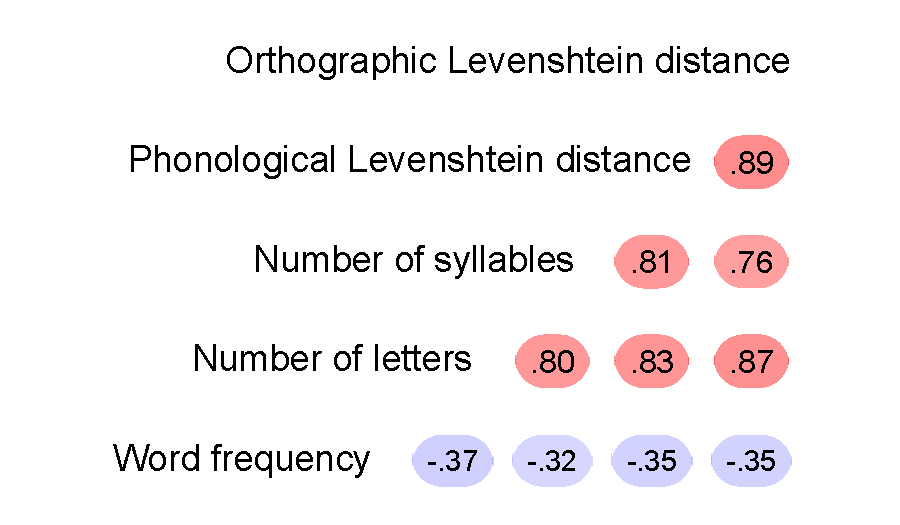
\includegraphics[width=0.5\linewidth]{manuscript_files/figure-latex/semanticpriming-lexical-covariates-correlations-1} 

}

\caption{Zero-order correlations among lexical covariates pretested in the semantic priming study.}\label{fig:semanticpriming-lexical-covariates-correlations}
\end{figure}

Table \ref{tab:semanticpriming-lexical-covariates-selection} shows the results of the selection model.

\begin{table}[H]

\caption{\label{tab:semanticpriming-lexical-covariates-selection}Mixed-effects model for the selection of lexical covariates in the semantic priming study.}
\centering
\begin{threeparttable}
\begin{tabular}[t]{lrrrrr}
\toprule
\multicolumn{1}{c}{ } & \multicolumn{1}{c}{$\upbeta$} & \multicolumn{1}{c}{$SE$} & \multicolumn{1}{c}{95\% CI} & \multicolumn{1}{c}{$t$} & \multicolumn{1}{c}{$p$}\\
\midrule
(Intercept) & 0.01 & 0.00 & {}[0.00, 0.02] & 1.19 & .236\\
Word frequency & -0.14 & 0.01 & {}[-0.15, -0.13] & -24.19 & <.001\\
Number of letters & 0.00 & 0.01 & {}[-0.02, 0.02] & 0.12 & .903\\
Number of syllables & 0.04 & 0.01 & {}[0.02, 0.06] & 4.02 & <.001\\
Orthographic Levenshtein distance & 0.03 & 0.01 & {}[0.00, 0.05] & 2.19 & .029\\
Phonological Levenshtein distance & 0.02 & 0.01 & {}[-0.01, 0.04] & 1.28 & .199\\
\bottomrule
\end{tabular}
\begin{tablenotes}
\item \textit{\linebreak} 
\item \textit{Note}. $\upbeta$ = Estimate based on z-scored variables; \textit{SE} = standard error; \linebreak \phantom{.}CI = confidence interval. By-participant random slopes were included for \linebreak \phantom{.}every effect.
\end{tablenotes}
\end{threeparttable}
\end{table}

Considering the maximum correlation allowed (\(r\) = \(\pm\).70) and the results of the model, the variables that will be included as covariates in the main analysis are word frequency and number of syllables.

\hypertarget{study-2-semantic-decision-1}{%
\subsection{Study 2: Semantic decision}\label{study-2-semantic-decision-1}}

Figure \ref{fig:semanticdecision-lexical-covariates-correlations} shows the zero-order correlations among the lexical covariates considered in the selection.

\begin{figure}

{\centering 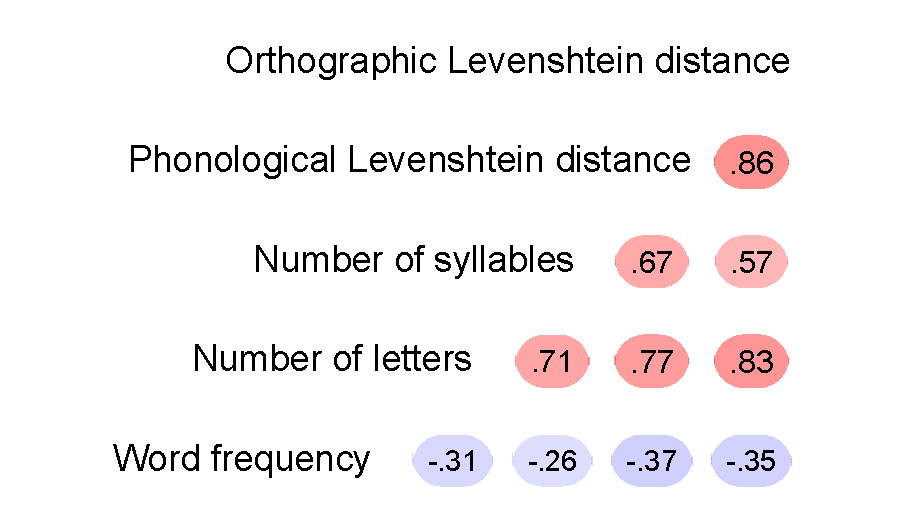
\includegraphics[width=0.5\linewidth]{manuscript_files/figure-latex/semanticdecision-lexical-covariates-correlations-1} 

}

\caption{Zero-order correlations for the lexical covariates pretested in the semantic decision study.}\label{fig:semanticdecision-lexical-covariates-correlations}
\end{figure}

Table \ref{tab:semanticdecision-lexical-covariates-selection} shows the results of the selection model.

\begin{table}[H]

\caption{\label{tab:semanticdecision-lexical-covariates-selection}Mixed-effects model for the selection of lexical covariates in the semantic decision study.}
\centering
\begin{threeparttable}
\begin{tabular}[t]{lrrrrr}
\toprule
\multicolumn{1}{c}{ } & \multicolumn{1}{c}{$\upbeta$} & \multicolumn{1}{c}{$SE$} & \multicolumn{1}{c}{95\% CI} & \multicolumn{1}{c}{$t$} & \multicolumn{1}{c}{$p$}\\
\midrule
(Intercept) & 0.05 & 0.00 & {}[0.05, 0.06] & 12.35 & <.001\\
Word frequency & -0.13 & 0.01 & {}[-0.14, -0.11] & -20.01 & <.001\\
Number of letters & 0.05 & 0.01 & {}[0.03, 0.07] & 5.20 & <.001\\
Number of syllables & 0.08 & 0.01 & {}[0.07, 0.10] & 10.80 & <.001\\
Orthographic Levenshtein distance & -0.13 & 0.01 & {}[-0.15, -0.10] & -10.23 & <.001\\
Phonological Levenshtein distance & 0.01 & 0.01 & {}[-0.01, 0.03] & 0.91 & .361\\
\bottomrule
\end{tabular}
\begin{tablenotes}
\item \textit{\linebreak} 
\item \textit{Note}. $\upbeta$ = Estimate based on z-scored variables; \textit{SE} = standard error; \linebreak \phantom{.}CI = confidence interval. By-participant random slopes were included for \linebreak \phantom{.}every effect.
\end{tablenotes}
\end{threeparttable}
\end{table}

Considering the maximum correlation allowed (\(r\) = \(\pm\).70) and the results of the model, the variables that will be included as covariates in the main analysis are word frequency and orthographic Levenshtein distance.

\hypertarget{study-3-lexical-decision-1}{%
\subsection{Study 3: Lexical decision}\label{study-3-lexical-decision-1}}

Figure \ref{fig:lexicaldecision-lexical-covariates-correlations} shows the zero-order correlations among the lexical covariates considered in the selection.

\begin{figure}

{\centering 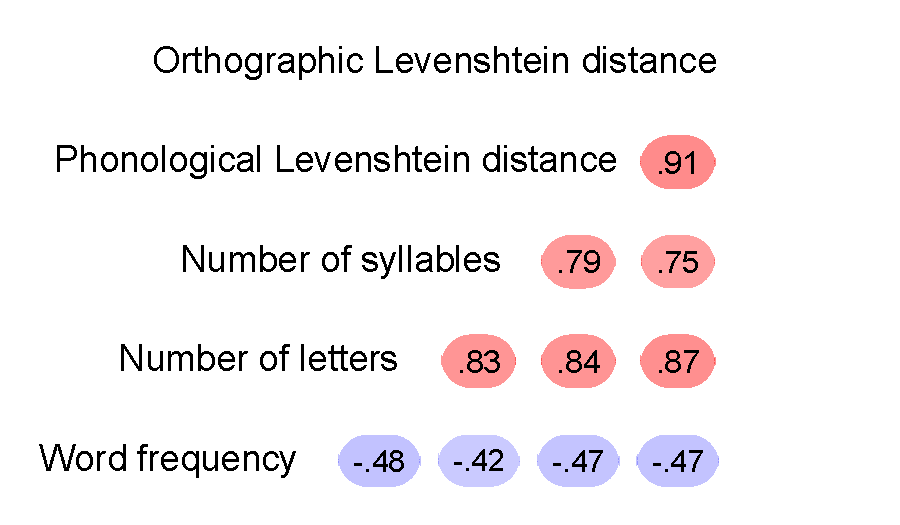
\includegraphics[width=0.5\linewidth]{manuscript_files/figure-latex/lexicaldecision-lexical-covariates-correlations-1} 

}

\caption{Zero-order correlations for the lexical covariates pretested in the lexical decision study.}\label{fig:lexicaldecision-lexical-covariates-correlations}
\end{figure}

Table \ref{tab:lexicaldecision-lexical-covariates-selection} shows the results of the selection model.

\begin{table}[H]

\caption{\label{tab:lexicaldecision-lexical-covariates-selection}Mixed-effects model for the selection of lexical covariates in the lexical decision study.}
\centering
\begin{threeparttable}
\begin{tabular}[t]{lrrrrr}
\toprule
\multicolumn{1}{c}{ } & \multicolumn{1}{c}{$\upbeta$} & \multicolumn{1}{c}{$SE$} & \multicolumn{1}{c}{95\% CI} & \multicolumn{1}{c}{$t$} & \multicolumn{1}{c}{$p$}\\
\midrule
(Intercept) & 0.00 & 0.01 & {}[-0.01, 0.01] & -0.02 & .981\\
Word frequency & -0.12 & 0.01 & {}[-0.15, -0.10] & -11.60 & <.001\\
Number of letters & 0.05 & 0.02 & {}[0.01, 0.09] & 2.73 & .006\\
Number of syllables & 0.06 & 0.01 & {}[0.03, 0.09] & 4.43 & <.001\\
Orthographic Levenshtein distance & 0.10 & 0.02 & {}[0.05, 0.14] & 4.52 & <.001\\
Phonological Levenshtein distance & -0.02 & 0.02 & {}[-0.06, 0.02] & -1.18 & .238\\
\bottomrule
\end{tabular}
\begin{tablenotes}
\item \textit{\linebreak} 
\item \textit{Note}. $\upbeta$ = Estimate based on z-scored variables; \textit{SE} = standard error; \linebreak \phantom{.}CI = confidence interval. By-participant random slopes were included for \linebreak \phantom{.}every effect.
\end{tablenotes}
\end{threeparttable}
\end{table}

Considering the maximum correlation allowed (\(r\) = \(\pm\).70), the results of the model, and the use of word frequency as a predictor of interest in the model, the variable that will be included as a covariate in the main analysis is orthographic Levenshtein distance.

\hypertarget{conclusion}{%
\subsection{Conclusion}\label{conclusion}}

Word frequency presented the largest effect in the three models. Orthographic Levenshtein distance was the second largest effect in the semantic decision and the lexical decision studies, whereas its phonological counterpart was not significant in any of the studies. The latter difference makes sense, as participants read the stimulus words in the three studies (Brysbaert, 2022).

\clearpage

\renewcommand{\thefigure}{B\arabic{figure}} \setcounter{figure}{0}
\renewcommand{\thetable}{B\arabic{table}} \setcounter{table}{0}

\hypertarget{appendix-B-frequentist-analysis-diagnostics}{%
\section{Appendix B: Diagnostics for the frequentist analyses}\label{appendix-B-frequentist-analysis-diagnostics}}

Below, the convergence warnings and the non-normal residuals are first addressed generally, and then in more detail in the context of each study.

\hypertarget{lack-of-convergence}{%
\subsection{Lack of convergence}\label{lack-of-convergence}}

The challenge of convergence is well known in the area of mixed-effects models. The solutions proposed range from the removal of random slopes under certain conditions (Matuschek et al., 2017) to the maintenance of random slopes in spite of convergence warnings, which seeks to avoid an inflation of the Type I error caused by non-independence in the data (Brauer \& Curtin, 2018; Singmann \& Kellen, 2019).

\hypertarget{the-multiple-optimizers-sanity-check-from-lme4allfit}{%
\subsubsection{\texorpdfstring{The multiple-optimizers sanity check from \texttt{lme4::allFit()}}{The multiple-optimizers sanity check from lme4::allFit()}}\label{the-multiple-optimizers-sanity-check-from-lme4allfit}}

Framed within the drive to maintain random slopes wherever possible, the developers of the `lme4' package propose a sanity check that uses a part of the `lme4' \emph{engine} called `optimizer'. Every model has a default optimizer, unless a specific one is chosen through \texttt{control\ =\ lmerControl(optimizer\ =\ \textquotesingle{}...\textquotesingle{})} (in \texttt{lmer} models) or \texttt{control\ =\ glmerControl(optimizer\ =\ \textquotesingle{}...\textquotesingle{})} (in \texttt{glmer} models). The 7 widely-available optimizers are:

\begin{itemize}
\tightlist
\item
  bobyqa
\item
  Nelder\_Mead
\item
  nlminbwrap
\item
  nmkbw
\item
  optimx.L-BFGS-B
\item
  nloptwrap.NLOPT\_LN\_NELDERMEAD
\item
  nloptwrap.NLOPT\_LN\_BOBYQA
\end{itemize}

To assess whether convergence warnings render the results invalid, or on the contrary, the results can be deemed valid in spite of the warnings, Bates et al. (2021) suggest refitting models affected by convergence warnings with a variety of optimizers. The authors argue that if the different optimizers produce practically-equivalent results, the results are valid. For this purpose, the `allFit' function from the `lme4' package allows the refitting of models using a number of optimizers. To use the 7 optimizers listed above, two extra packages were installed: `dfoptim' and `optimx' (see \href{https://cran.r-project.org/web/packages/lme4/lme4.pdf}{lme4 manual}). The output from `allFit' contains several statistics on the fixed and the random effects fitted by each optimizer (see \href{https://github.com/lme4/lme4/issues/512\#issue-425198940}{example}).

The severity of convergence problems in each study will be examined below using the `allFit' function from the `lme4' package.

\hypertarget{residual-errors-not-normally-distributed}{%
\subsection{Residual errors not normally distributed}\label{residual-errors-not-normally-distributed}}

The residuals of the linear mixed-effects models in all three studies violated the assumption of normality. Even though linear mixed-effects models tend to be quite robust to deviations from normality (Knief \& Forstmeier, 2021; Schielzeth et al., 2020), we sought to verify our results. To this end, two robust models were performed in each study, as described below.

\hypertarget{method-a-robustlmm-model}{%
\subsubsection{\texorpdfstring{Method A: \emph{robustlmm} model}{Method A: robustlmm model}}\label{method-a-robustlmm-model}}

The first method uses the R package `robustlmm' v2.4-4 (Koller, 2016). To calculate the p values, we followed the procedure of Sleegers et al. (2021), but used the Kenward-Roger method instead of Satterthwaite (see Luke, 2017).

\hypertarget{method-b-inverse-gaussian-model-with-identity-link-function}{%
\subsubsection{Method B: Inverse Gaussian model with identity link function}\label{method-b-inverse-gaussian-model-with-identity-link-function}}

We followed a method proposed by Lo and Andrews (2015), based on generalized linear mixed-effects models (GLMM) implementing an identity link function. According to Lo and Andrews (2015), the link function helps avoid directly transforming the dependent variable, which can hinder the interpretability of the results (also see Knief \& Forstmeier, 2021).

GLMMs require the use of families of distributions. Lo and Andrews (2015) tested the Gaussian, Gamma and Inverse Gaussian families, with either an identity or an inverse link function. The authors found that the Inverse Gaussian family with an identity link yielded the most normal residuals. The Inverse Gaussian and the Gamma families only accept positive values in the outcome variable (see Table 15.2 in Fox, 2016). Due to this restriction, the dependent variable in the present model is raw RT, unlike the standardised RT that was used in the main analysis.

\emph{P} values were to be calculated through parametric bootstrapping, which is the most robust method for GLMMs, as the Kenward-Roger and Satterthwaite methods are not available for these models (Luke, 2017; Singmann et al., 2021).

Neither Method A nor Method B could finally be used, as the code produced errors. These errors are shown in the corresponding scripts inside the `model\_diagnostics' folder in each study. Nonetheless, the residuals are shown below.

\hypertarget{study-1-semantic-priming-2}{%
\subsection{Study 1: Semantic priming}\label{study-1-semantic-priming-2}}

\hypertarget{lack-of-convergence-1}{%
\subsubsection{Lack of convergence}\label{lack-of-convergence-1}}

In the initial model, the optimizer used (the default one in `lmerTest') was `nloptwrap', and the convergence warning read: `boundary (singular) fit: see ?isSingular'.

Based on the reanalysis using 7 optimizers, Figure \ref{fig:main-effects-semanticpriming-allFit-convergence} shows the fixed, main effects, and Figure \ref{fig:interactions-semanticpriming-allFit-convergence} shows the fixed interactions.

\begin{figure}

{\centering 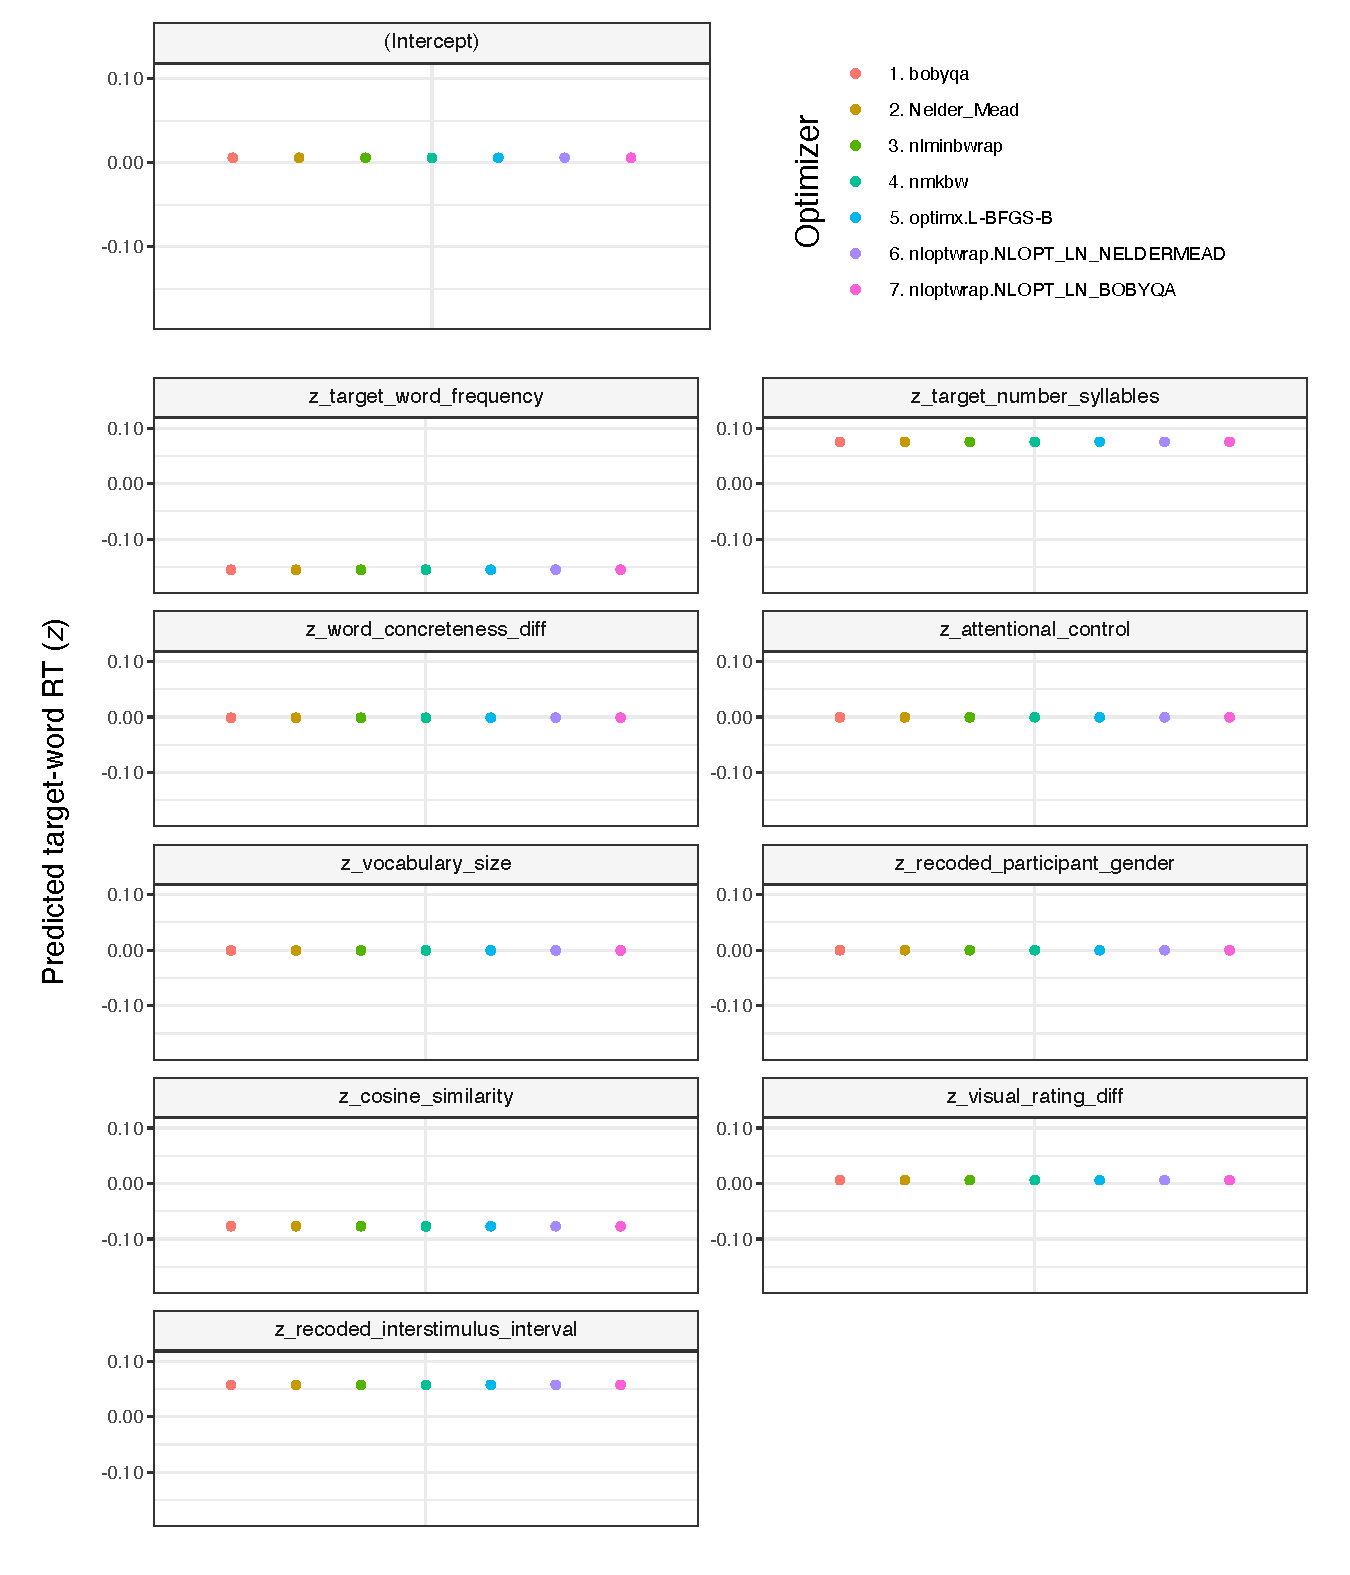
\includegraphics[width=1\linewidth]{/Users/pablodejuanbernabeu/Library/CloudStorage/OneDrive-LancasterUniversity/semanticpriming-semanticdecision-lexicaldecision/semanticpriming/frequentist_analysis/model_diagnostics/plots/main_effects_semanticpriming_allFit_convergence} 

}

\caption{Fixed, main effects from the semantic priming study fitted by 7 optimizers.}\label{fig:main-effects-semanticpriming-allFit-convergence}
\end{figure}

\begin{figure}

{\centering 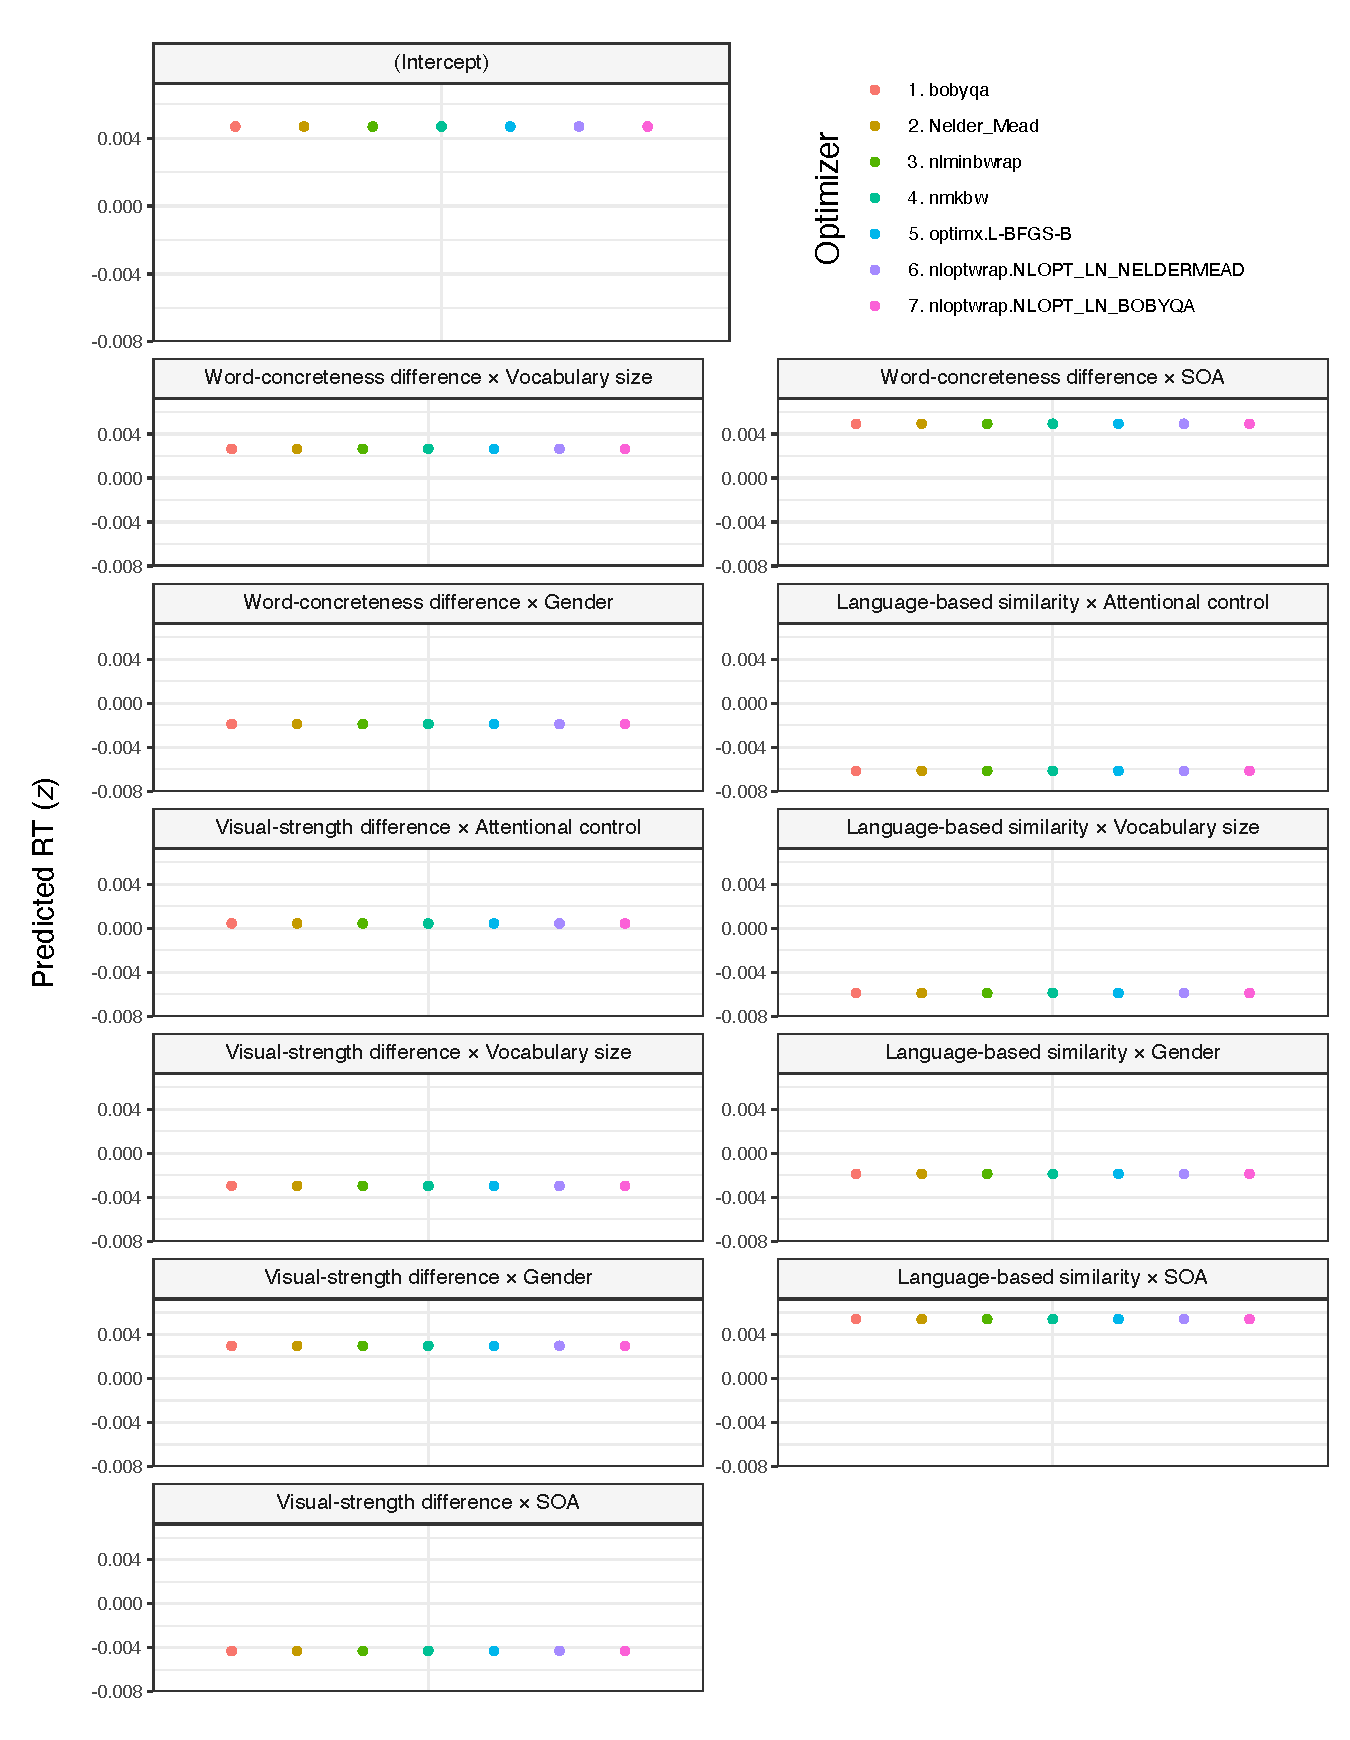
\includegraphics[width=1\linewidth]{/Users/pablodejuanbernabeu/Library/CloudStorage/OneDrive-LancasterUniversity/semanticpriming-semanticdecision-lexicaldecision/semanticpriming/frequentist_analysis/model_diagnostics/plots/interactions_semanticpriming_allFit_convergence} 

}

\caption{Fixed interaction effects from the semantic priming study fitted by 7 optimizers.}\label{fig:interactions-semanticpriming-allFit-convergence}
\end{figure}

\hypertarget{residual-errors-not-normally-distributed-1}{%
\subsubsection{Residual errors not normally distributed}\label{residual-errors-not-normally-distributed-1}}

Figure \ref{fig:semanticpriming-residuals} shows the deviation from normality of the residuals of the linear mixed-effects model.

\begin{figure}

{\centering 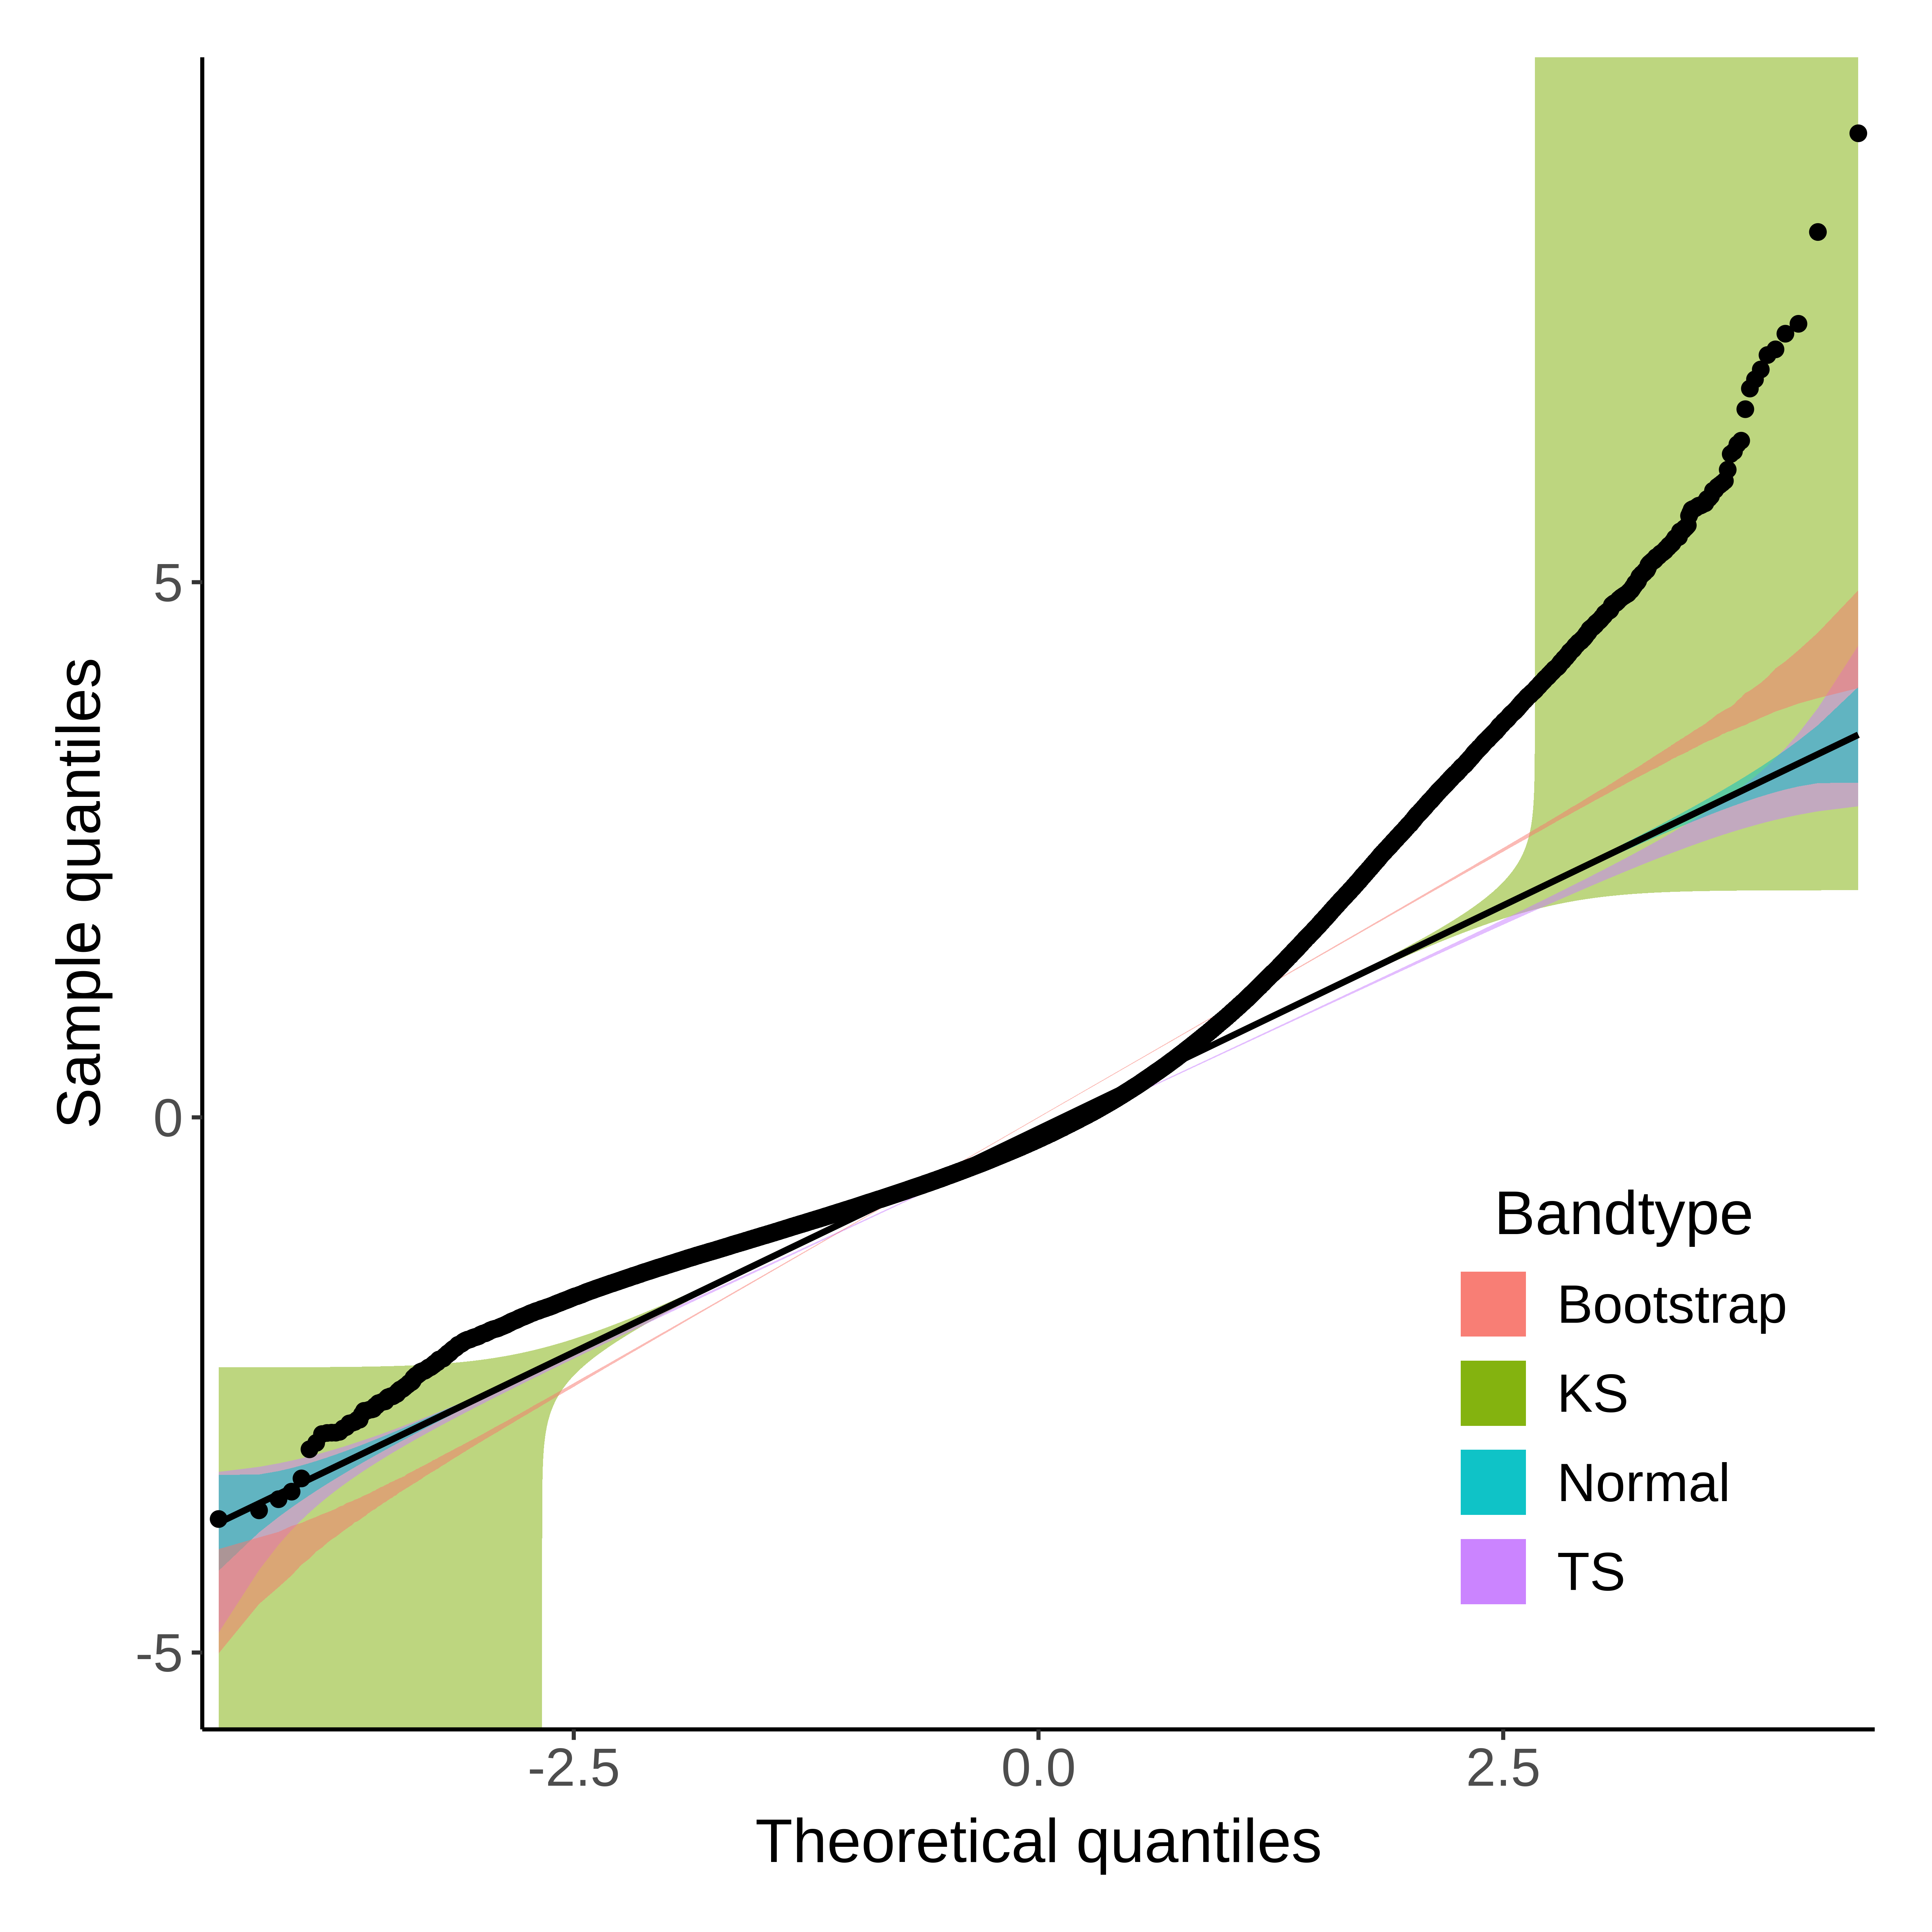
\includegraphics[width=0.65\linewidth]{/Users/pablodejuanbernabeu/Library/CloudStorage/OneDrive-LancasterUniversity/semanticpriming-semanticdecision-lexicaldecision/semanticpriming/frequentist_analysis/model_diagnostics/plots/semanticpriming_residuals} 

}

\caption{Residuals of the linear mixed-effects model from the semantic priming study. \linebreak KS = Kolmogorov-Smirnov test; TS = tail-sensitive confidence bands.}\label{fig:semanticpriming-residuals}
\end{figure}

\hypertarget{semantic-priming-model-including-visual-similarity}{%
\subsubsection{Semantic priming model including visual similarity}\label{semantic-priming-model-including-visual-similarity}}

\hypertarget{convergence}{%
\paragraph{Convergence}\label{convergence}}

In the initial model, the optimizer used (the default one in `lmerTest') was `nloptwrap', and the convergence warning read: `boundary (singular) fit: see ?isSingular'.

Based on the reanalysis using 7 optimizers, Figure \ref{fig:main-effects-semanticpriming-with-visualsimilarity-allFit-convergence} shows the fixed, main effects, and Figure \ref{fig:interactions-semanticpriming-with-visualsimilarity-allFit-convergence} shows the fixed interactions.

\begin{figure}

{\centering 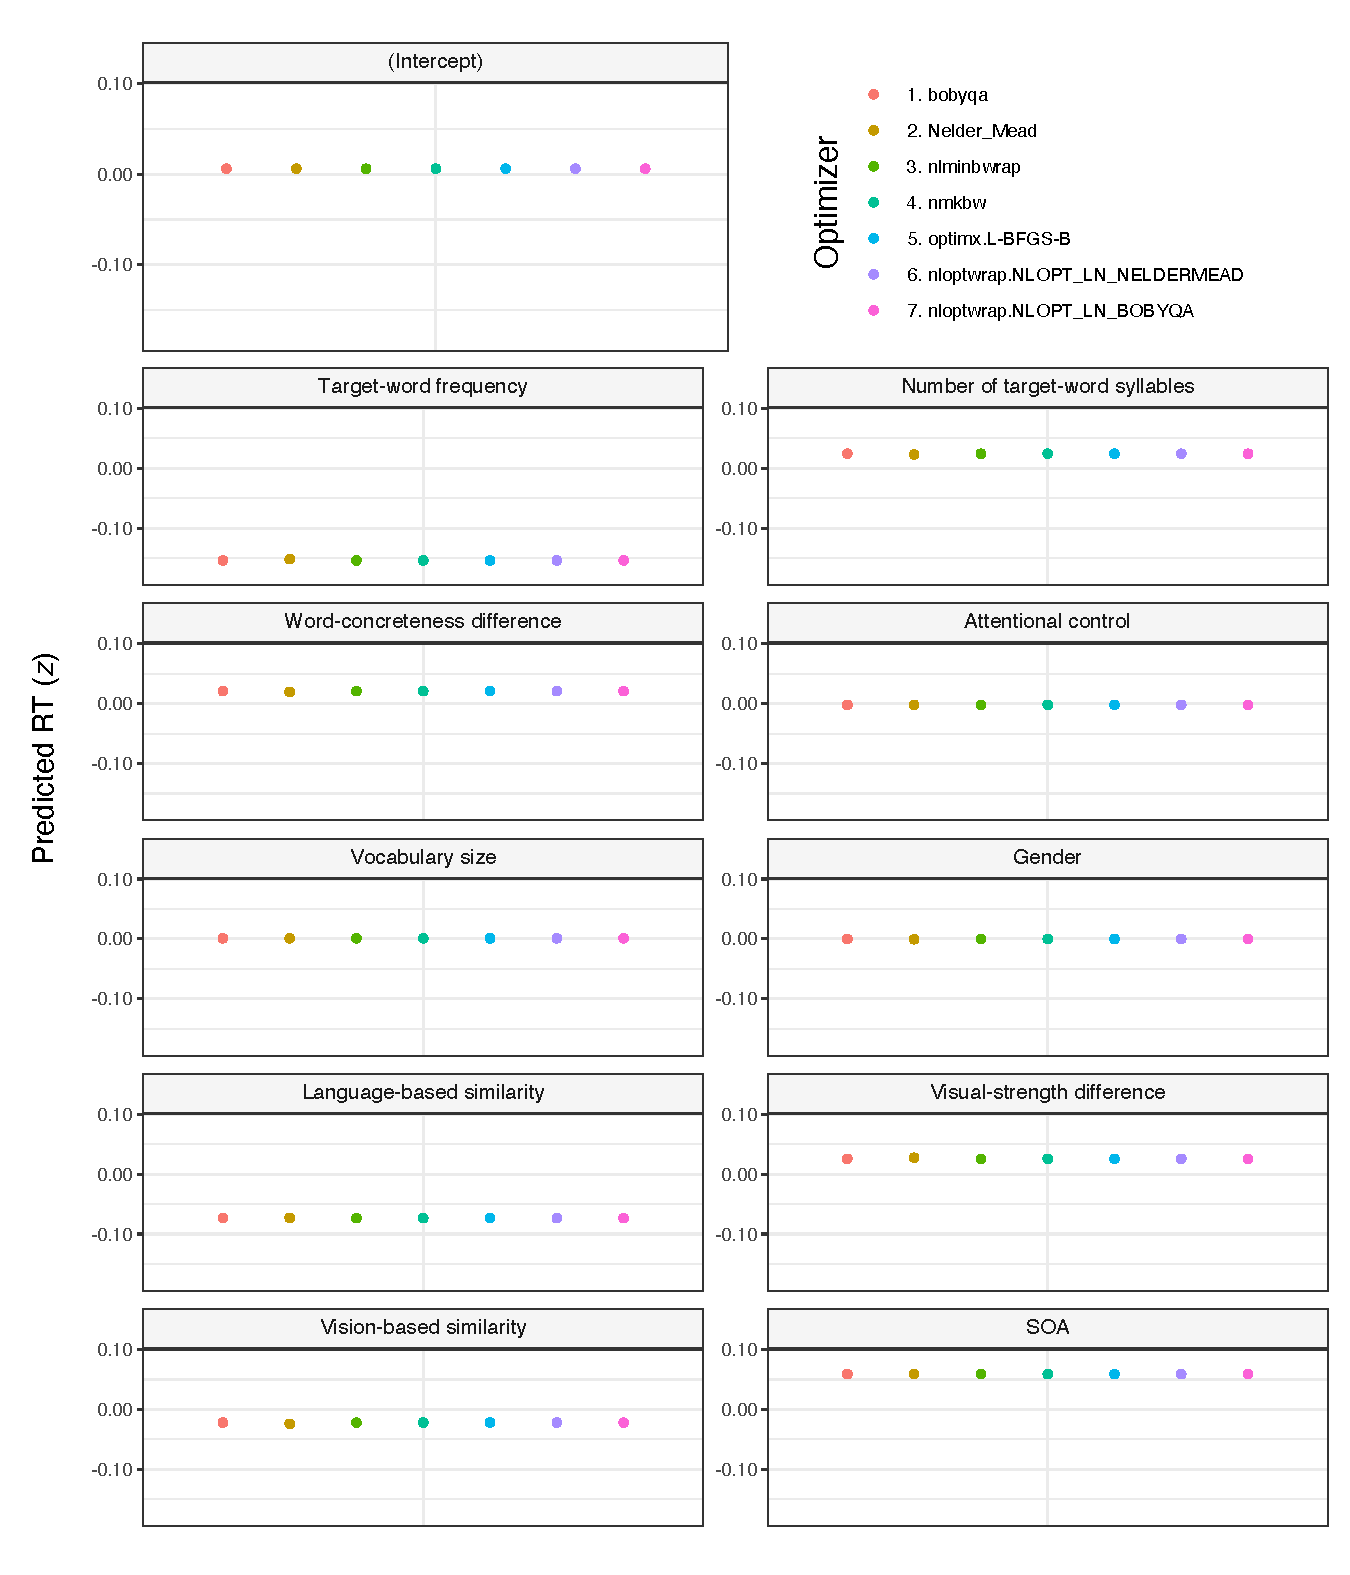
\includegraphics[width=1\linewidth]{/Users/pablodejuanbernabeu/Library/CloudStorage/OneDrive-LancasterUniversity/semanticpriming-semanticdecision-lexicaldecision/semanticpriming/analysis_with_visualsimilarity/model_diagnostics/plots/main_effects_semanticpriming_with_visualsimilarity_allFit_convergence} 

}

\caption{Fixed, main effects from the semantic priming study fitted by 7 optimizers.}\label{fig:main-effects-semanticpriming-with-visualsimilarity-allFit-convergence}
\end{figure}

\begin{figure}

{\centering 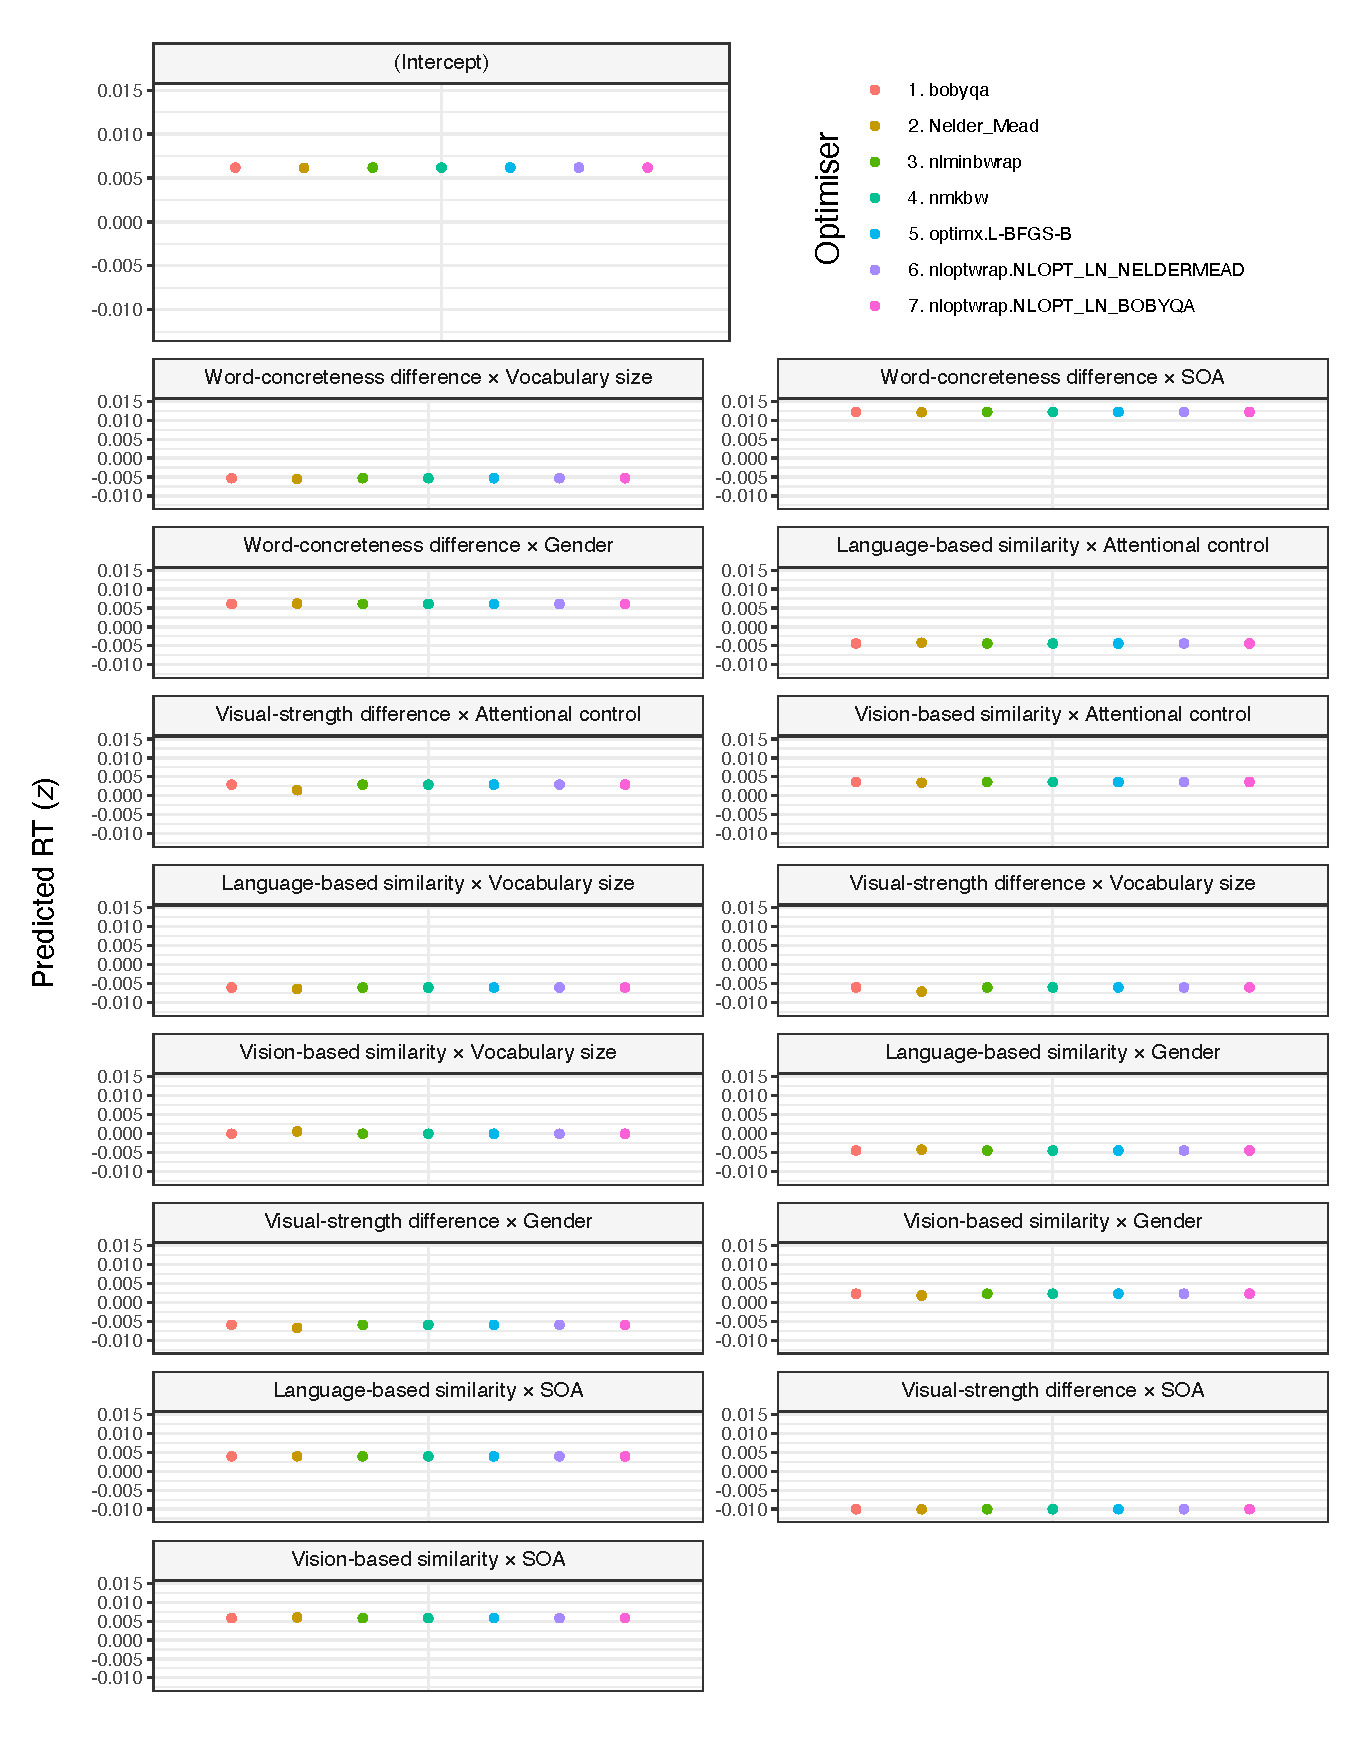
\includegraphics[width=1\linewidth]{/Users/pablodejuanbernabeu/Library/CloudStorage/OneDrive-LancasterUniversity/semanticpriming-semanticdecision-lexicaldecision/semanticpriming/analysis_with_visualsimilarity/model_diagnostics/plots/interactions_semanticpriming_with_visualsimilarity_allFit_convergence} 

}

\caption{Fixed interaction effects from the semantic priming study fitted by 7 optimizers.}\label{fig:interactions-semanticpriming-with-visualsimilarity-allFit-convergence}
\end{figure}

\hypertarget{residual-errors-not-normally-distributed-2}{%
\paragraph{Residual errors not normally distributed}\label{residual-errors-not-normally-distributed-2}}

Figure \ref{fig:semanticpriming-with-visualsimilarity-residuals} shows the deviation from normality of the residuals of the linear mixed-effects model.

\begin{figure}

{\centering 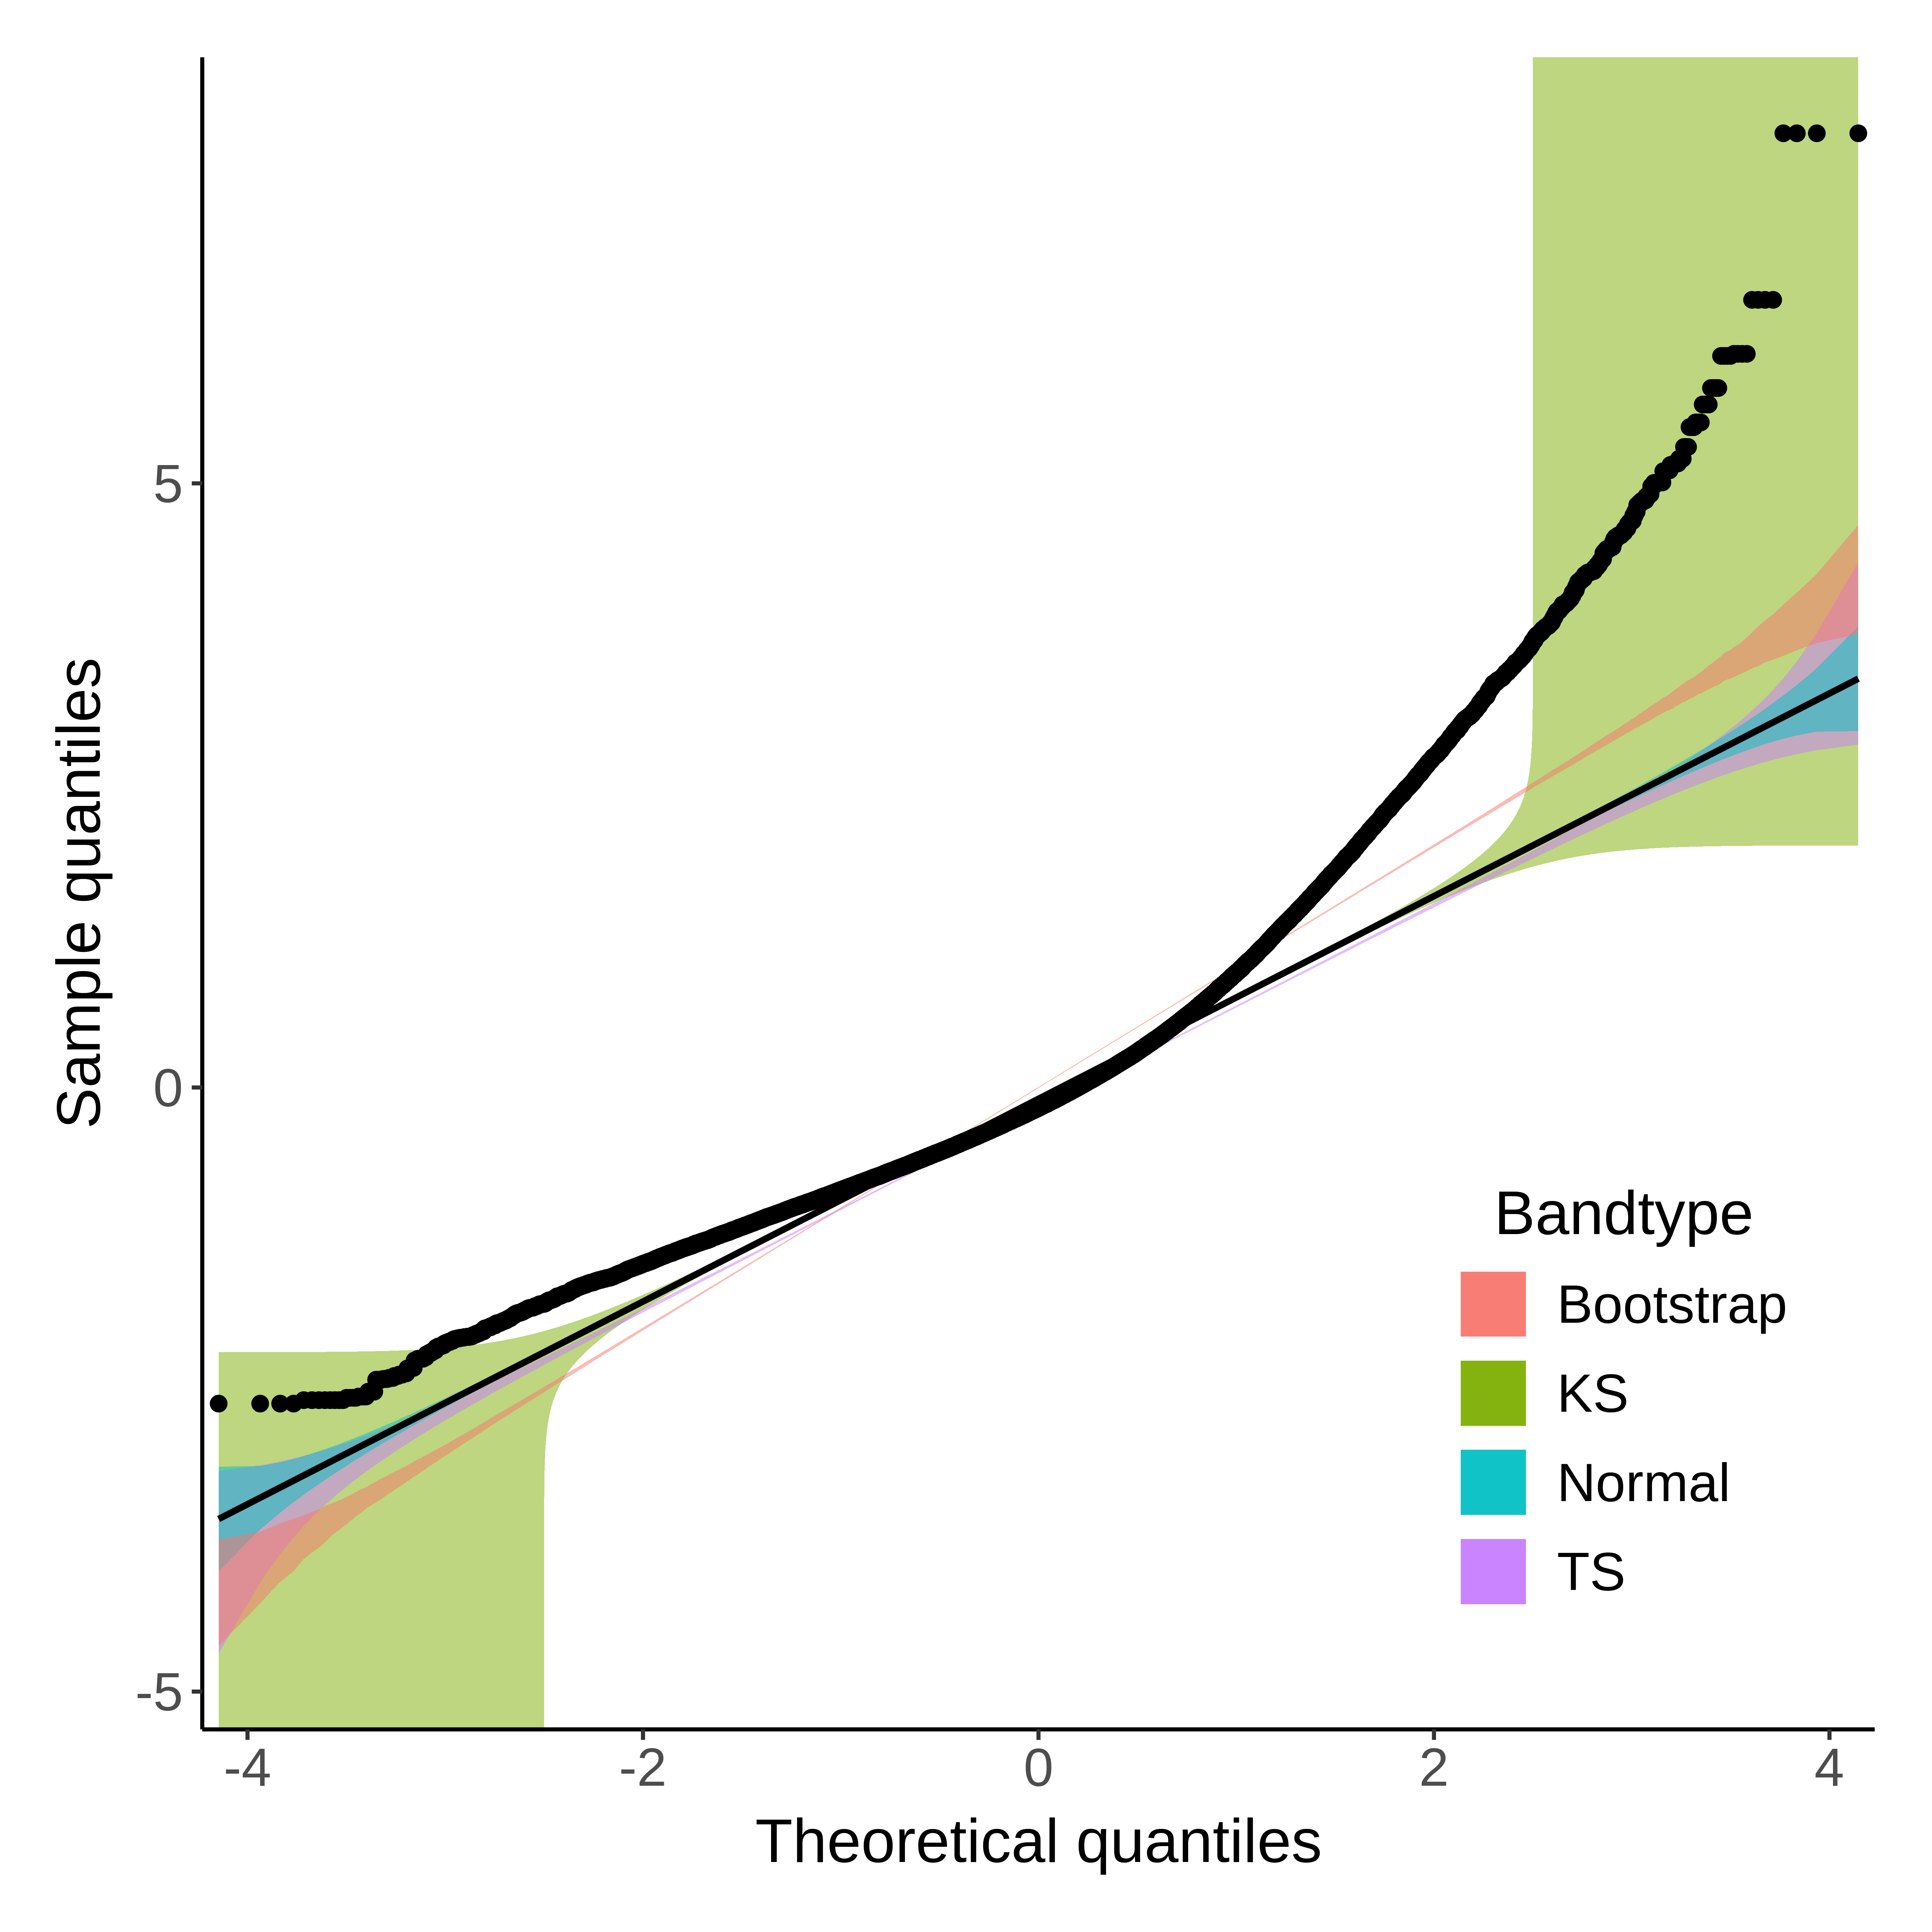
\includegraphics[width=0.65\linewidth]{/Users/pablodejuanbernabeu/Library/CloudStorage/OneDrive-LancasterUniversity/semanticpriming-semanticdecision-lexicaldecision/semanticpriming/analysis_with_visualsimilarity/model_diagnostics/plots/semanticpriming_with_visualsimilarity_residuals} 

}

\caption{Residuals of the linear mixed-effects model from the semantic priming study. \linebreak KS = Kolmogorov-Smirnov test; TS = tail-sensitive confidence bands.}\label{fig:semanticpriming-with-visualsimilarity-residuals}
\end{figure}

\hypertarget{study-2-semantic-decision-2}{%
\subsection{Study 2: Semantic decision}\label{study-2-semantic-decision-2}}

\hypertarget{convergence-1}{%
\subsubsection{Convergence}\label{convergence-1}}

In the initial model, the optimizer used (the default one in `lmerTest') was `nloptwrap', and the convergence warning read: `boundary (singular) fit: see ?isSingular'.

Based on the reanalysis using 7 optimizers, Figure \ref{fig:main-effects-semanticdecision-allFit-convergence} shows the fixed, main effects, and Figure \ref{fig:interactions-semanticdecision-allFit-convergence} shows the fixed interactions.

\begin{figure}

{\centering 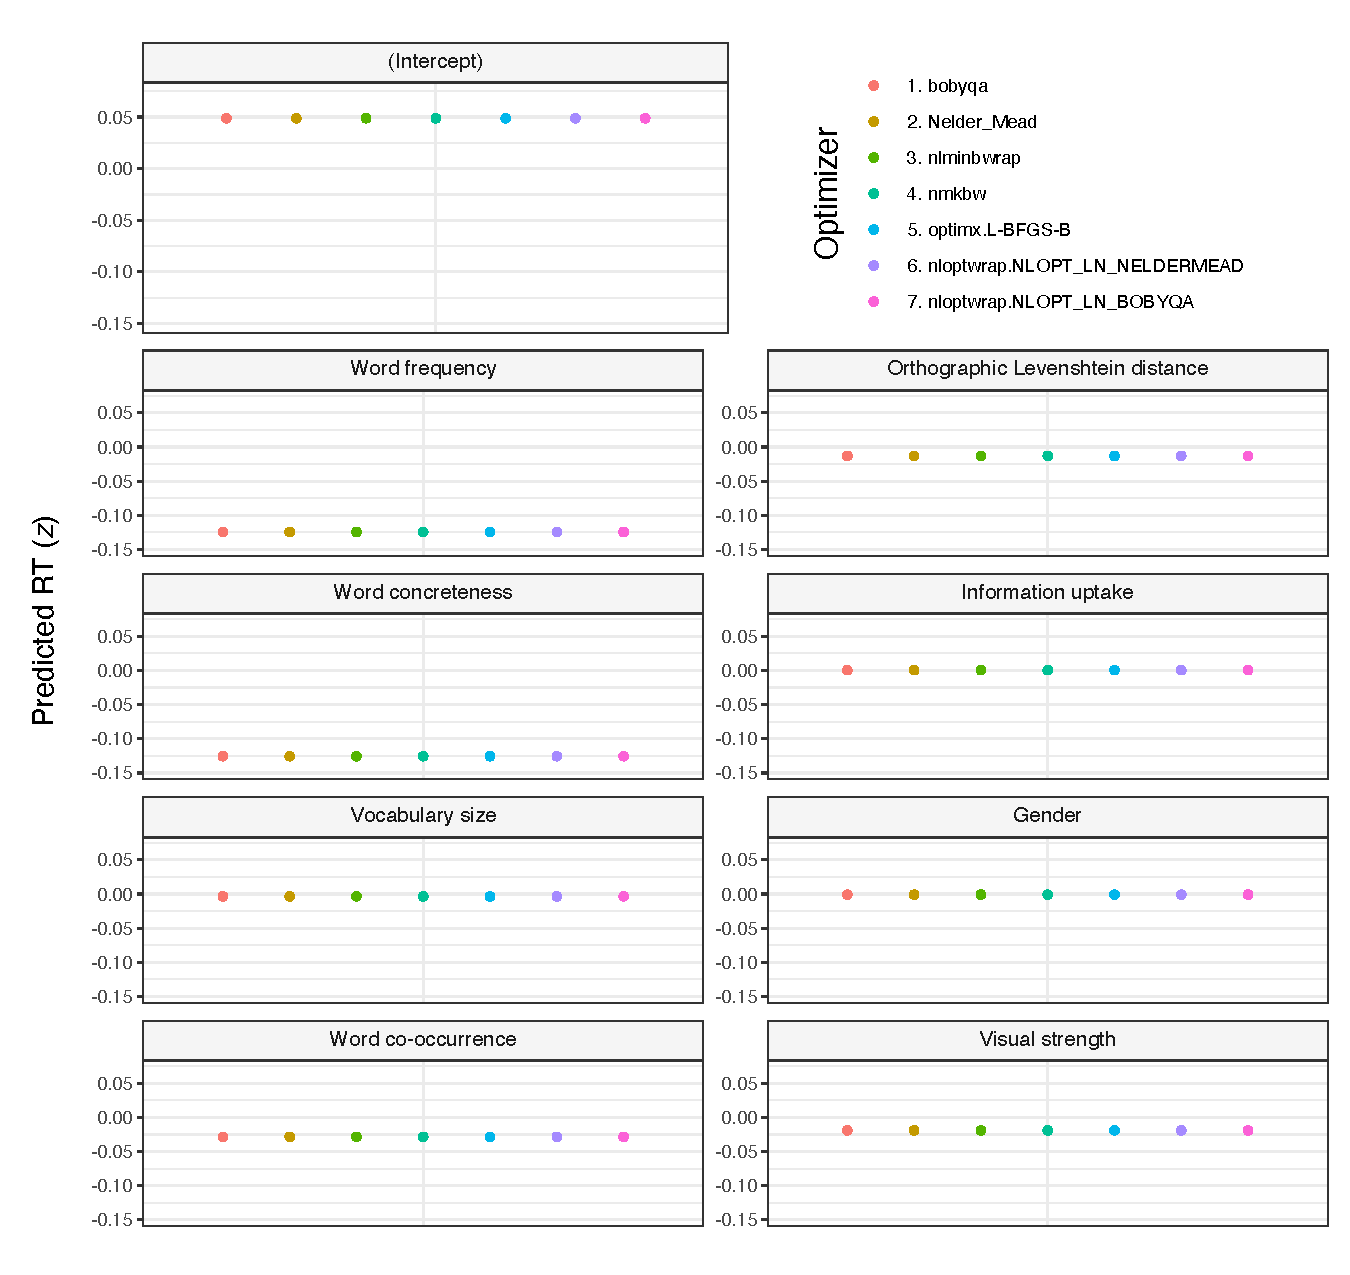
\includegraphics[width=1\linewidth]{/Users/pablodejuanbernabeu/Library/CloudStorage/OneDrive-LancasterUniversity/semanticpriming-semanticdecision-lexicaldecision/semanticdecision/frequentist_analysis/model_diagnostics/plots/main_effects_semanticdecision_allFit_convergence} 

}

\caption{Fixed, main effects from the semantic decision study fitted by 7 optimizers.}\label{fig:main-effects-semanticdecision-allFit-convergence}
\end{figure}

\begin{figure}

{\centering 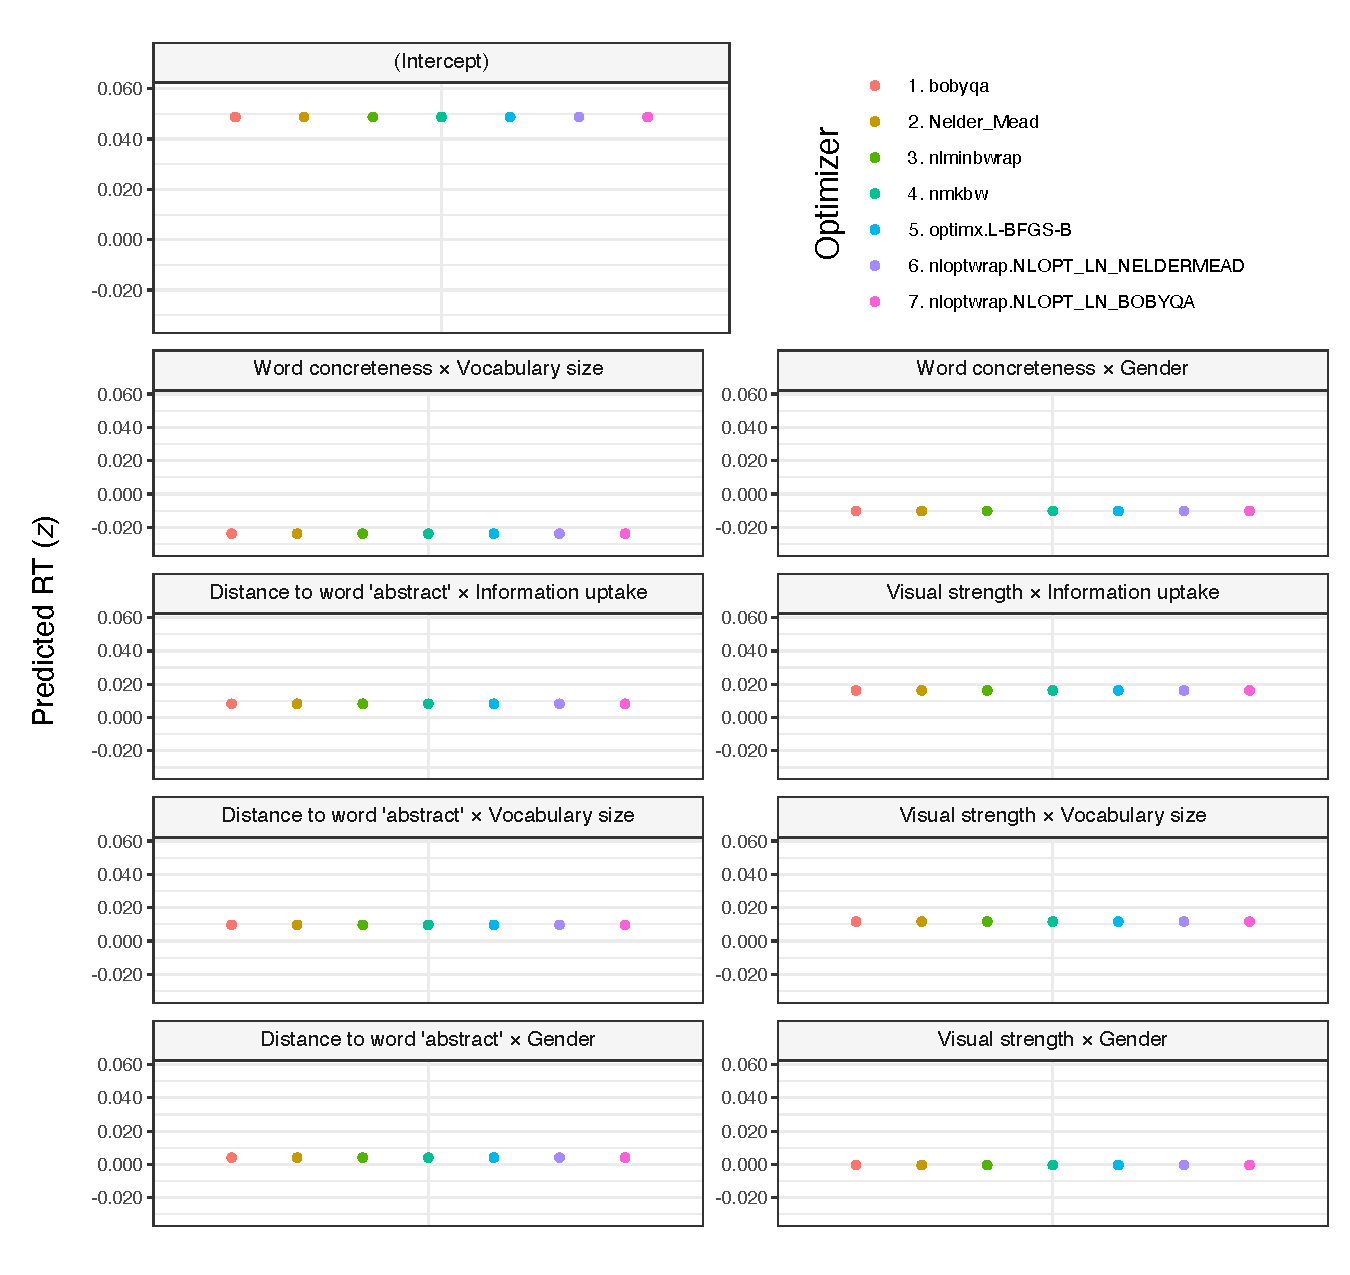
\includegraphics[width=1\linewidth]{/Users/pablodejuanbernabeu/Library/CloudStorage/OneDrive-LancasterUniversity/semanticpriming-semanticdecision-lexicaldecision/semanticdecision/frequentist_analysis/model_diagnostics/plots/interactions_semanticdecision_allFit_convergence} 

}

\caption{Fixed interaction effects from the semantic decision study fitted by 7 optimizers.}\label{fig:interactions-semanticdecision-allFit-convergence}
\end{figure}

\hypertarget{residual-errors-not-normally-distributed-3}{%
\subsubsection{Residual errors not normally distributed}\label{residual-errors-not-normally-distributed-3}}

Figure \ref{fig:semanticdecision-residuals} shows the deviation from normality of the residuals.

\begin{figure}

{\centering 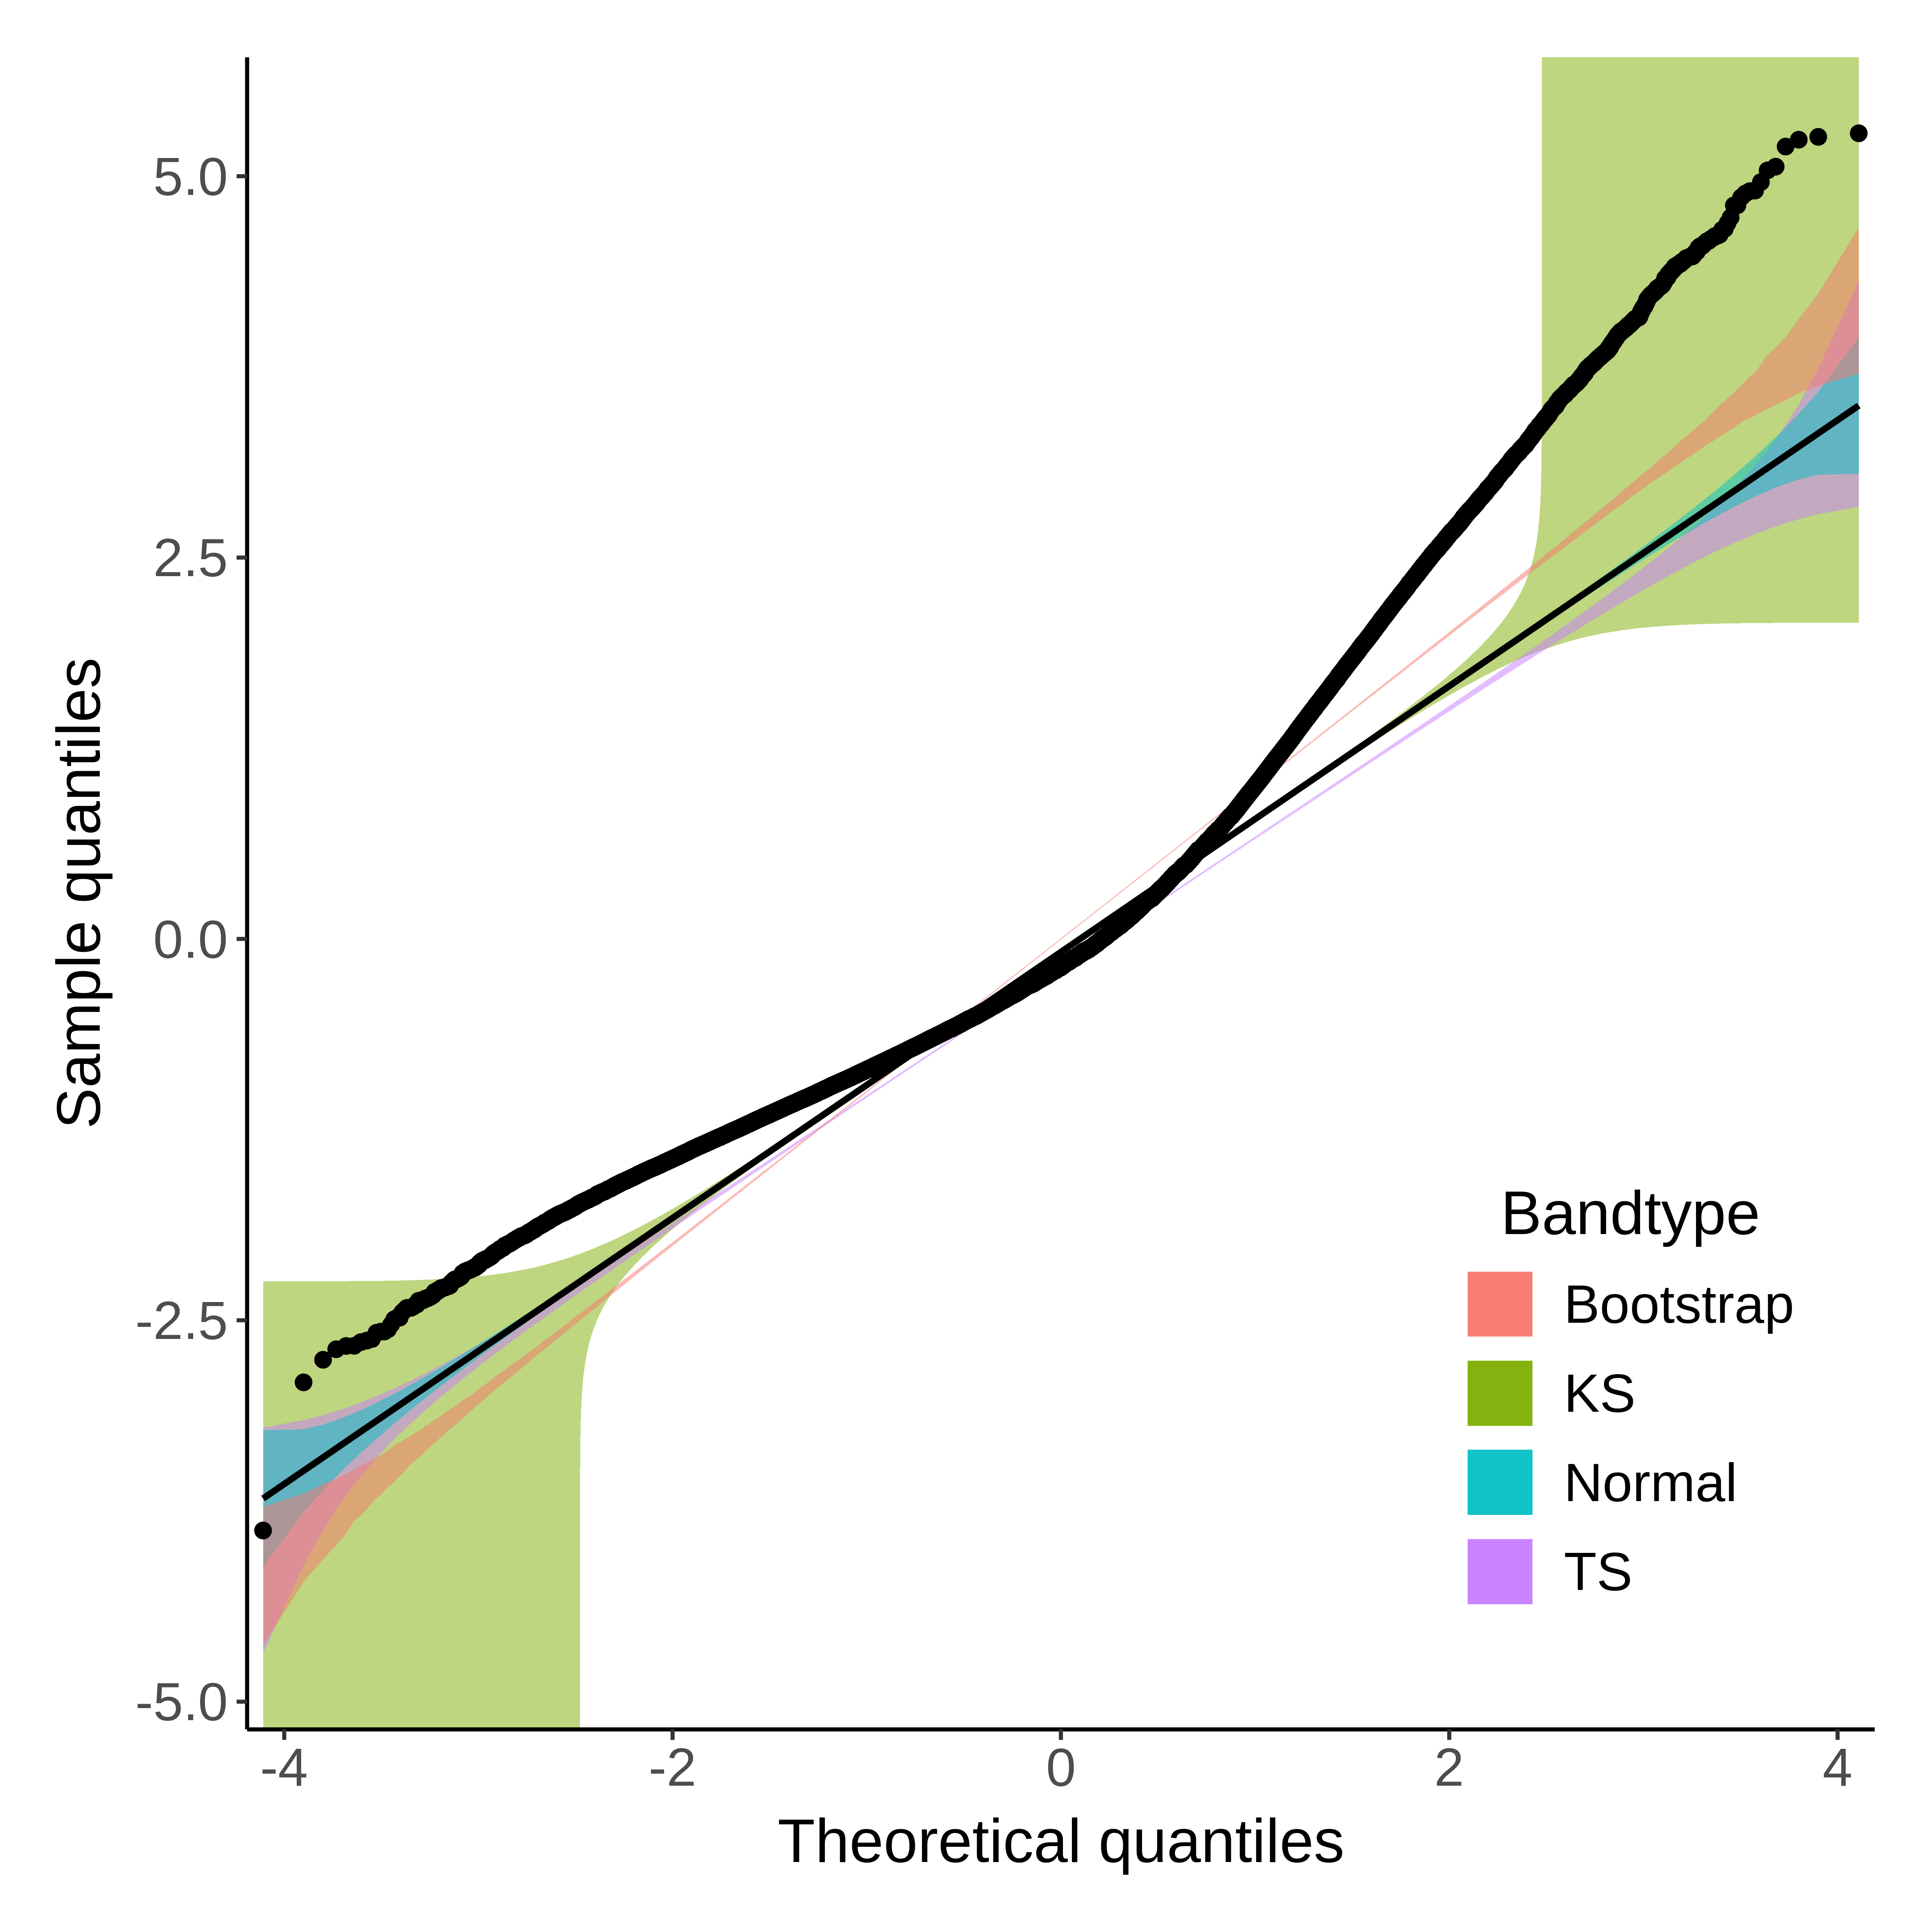
\includegraphics[width=0.65\linewidth]{/Users/pablodejuanbernabeu/Library/CloudStorage/OneDrive-LancasterUniversity/semanticpriming-semanticdecision-lexicaldecision/semanticdecision/frequentist_analysis/model_diagnostics/plots/semanticdecision_residuals} 

}

\caption{Residuals of the linear mixed-effects model from the semantic decision study. \linebreak KS = Kolmogorov-Smirnov test; TS = tail-sensitive confidence bands.}\label{fig:semanticdecision-residuals}
\end{figure}

\hypertarget{study-3-lexical-decision-2}{%
\subsection{Study 3: Lexical decision}\label{study-3-lexical-decision-2}}

\hypertarget{convergence-2}{%
\subsubsection{Convergence}\label{convergence-2}}

In the initial model, the optimizer used (the default one in `lmerTest') was `nloptwrap', and the convergence warning read: `boundary (singular) fit: see ?isSingular'.

Based on the reanalysis using 7 optimizers, Figure \ref{fig:main-effects-lexicaldecision-allFit-convergence} shows the fixed, main effects, and Figure \ref{fig:interactions-lexicaldecision-allFit-convergence} shows the fixed interactions.

\begin{figure}

{\centering 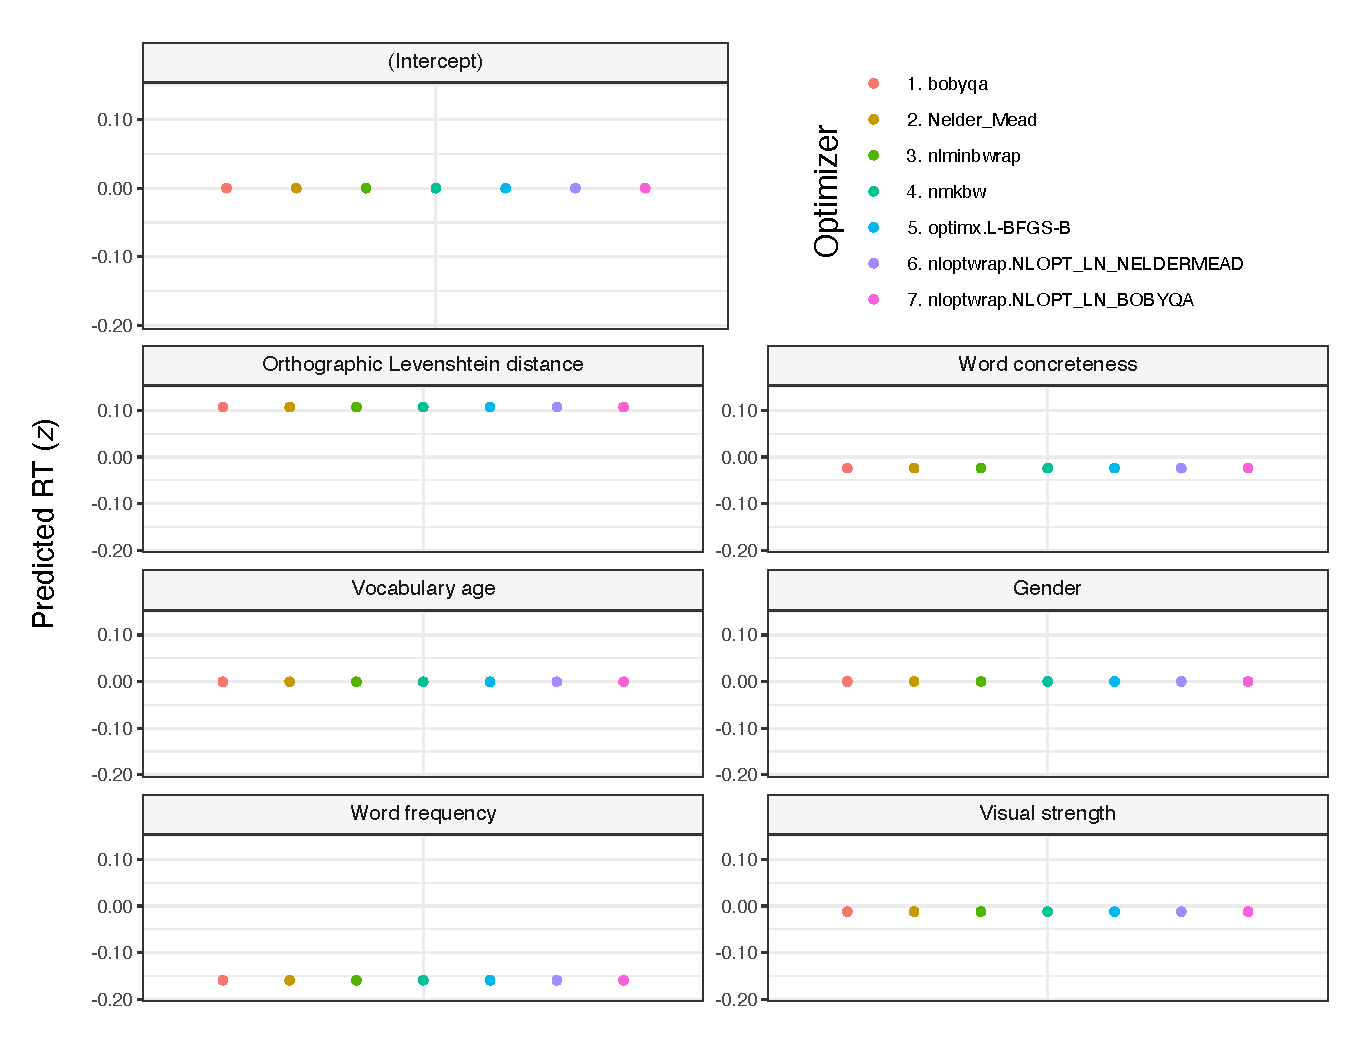
\includegraphics[width=1\linewidth]{/Users/pablodejuanbernabeu/Library/CloudStorage/OneDrive-LancasterUniversity/semanticpriming-semanticdecision-lexicaldecision/lexicaldecision/frequentist_analysis/model_diagnostics/plots/main_effects_lexicaldecision_allFit_convergence} 

}

\caption{Fixed, main effects from the lexical decision study fitted by 7 optimizers.}\label{fig:main-effects-lexicaldecision-allFit-convergence}
\end{figure}

\begin{figure}

{\centering 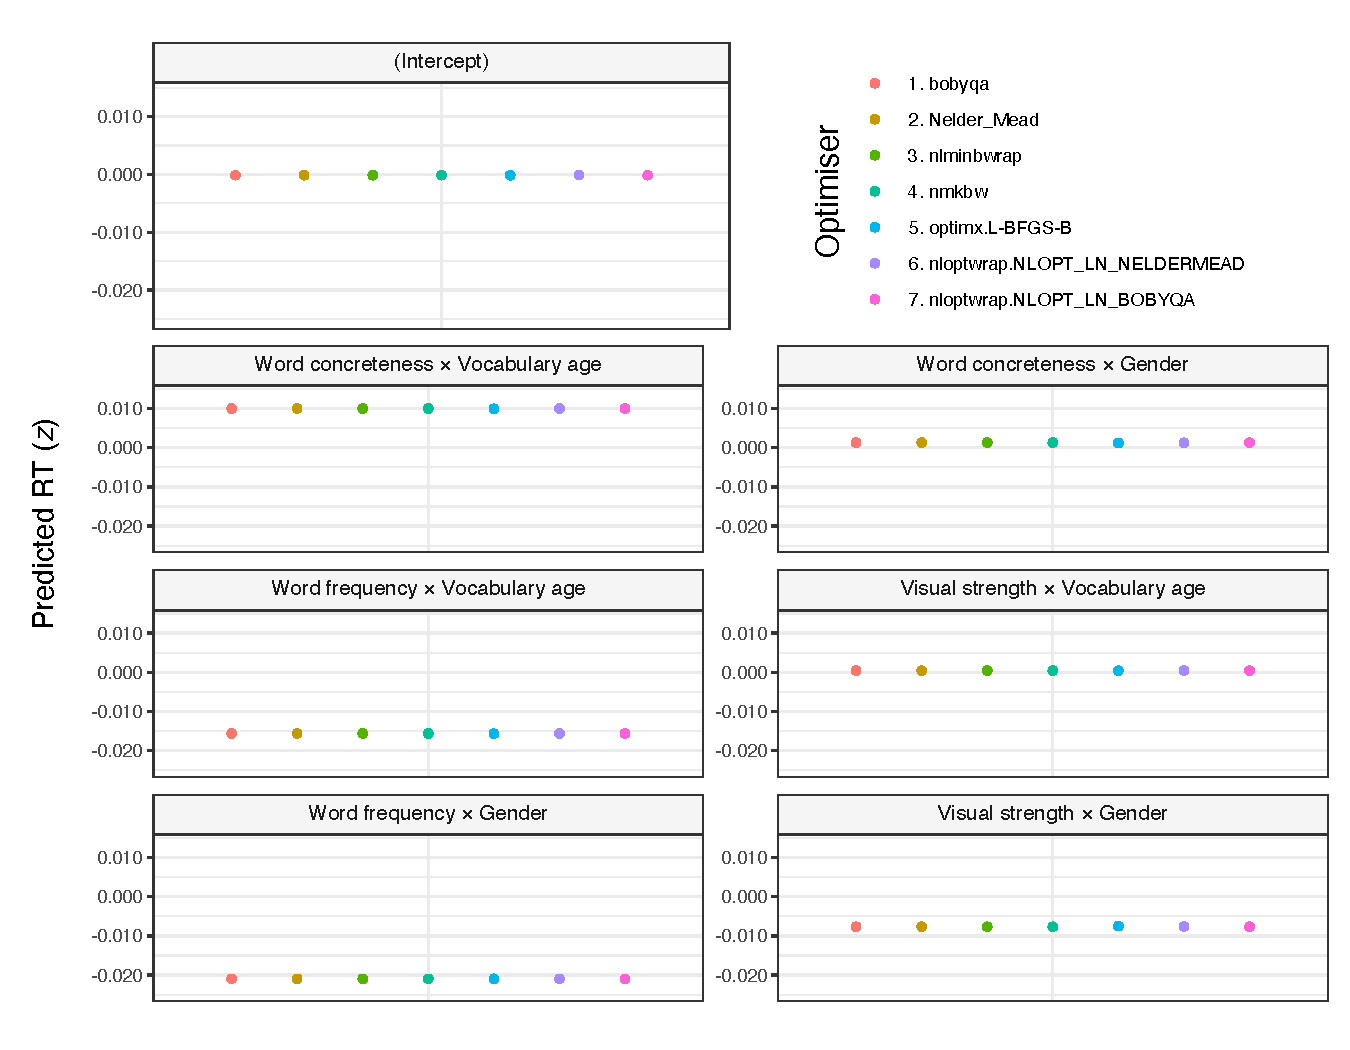
\includegraphics[width=1\linewidth]{/Users/pablodejuanbernabeu/Library/CloudStorage/OneDrive-LancasterUniversity/semanticpriming-semanticdecision-lexicaldecision/lexicaldecision/frequentist_analysis/model_diagnostics/plots/interactions_lexicaldecision_allFit_convergence} 

}

\caption{Fixed interaction effects from the lexical decision study fitted by 7 optimizers.}\label{fig:interactions-lexicaldecision-allFit-convergence}
\end{figure}

\hypertarget{residual-errors-not-normally-distributed-4}{%
\subsubsection{Residual errors not normally distributed}\label{residual-errors-not-normally-distributed-4}}

Figure \ref{fig:lexicaldecision-residuals} shows the deviation from normality of the residuals.

\begin{figure}

{\centering 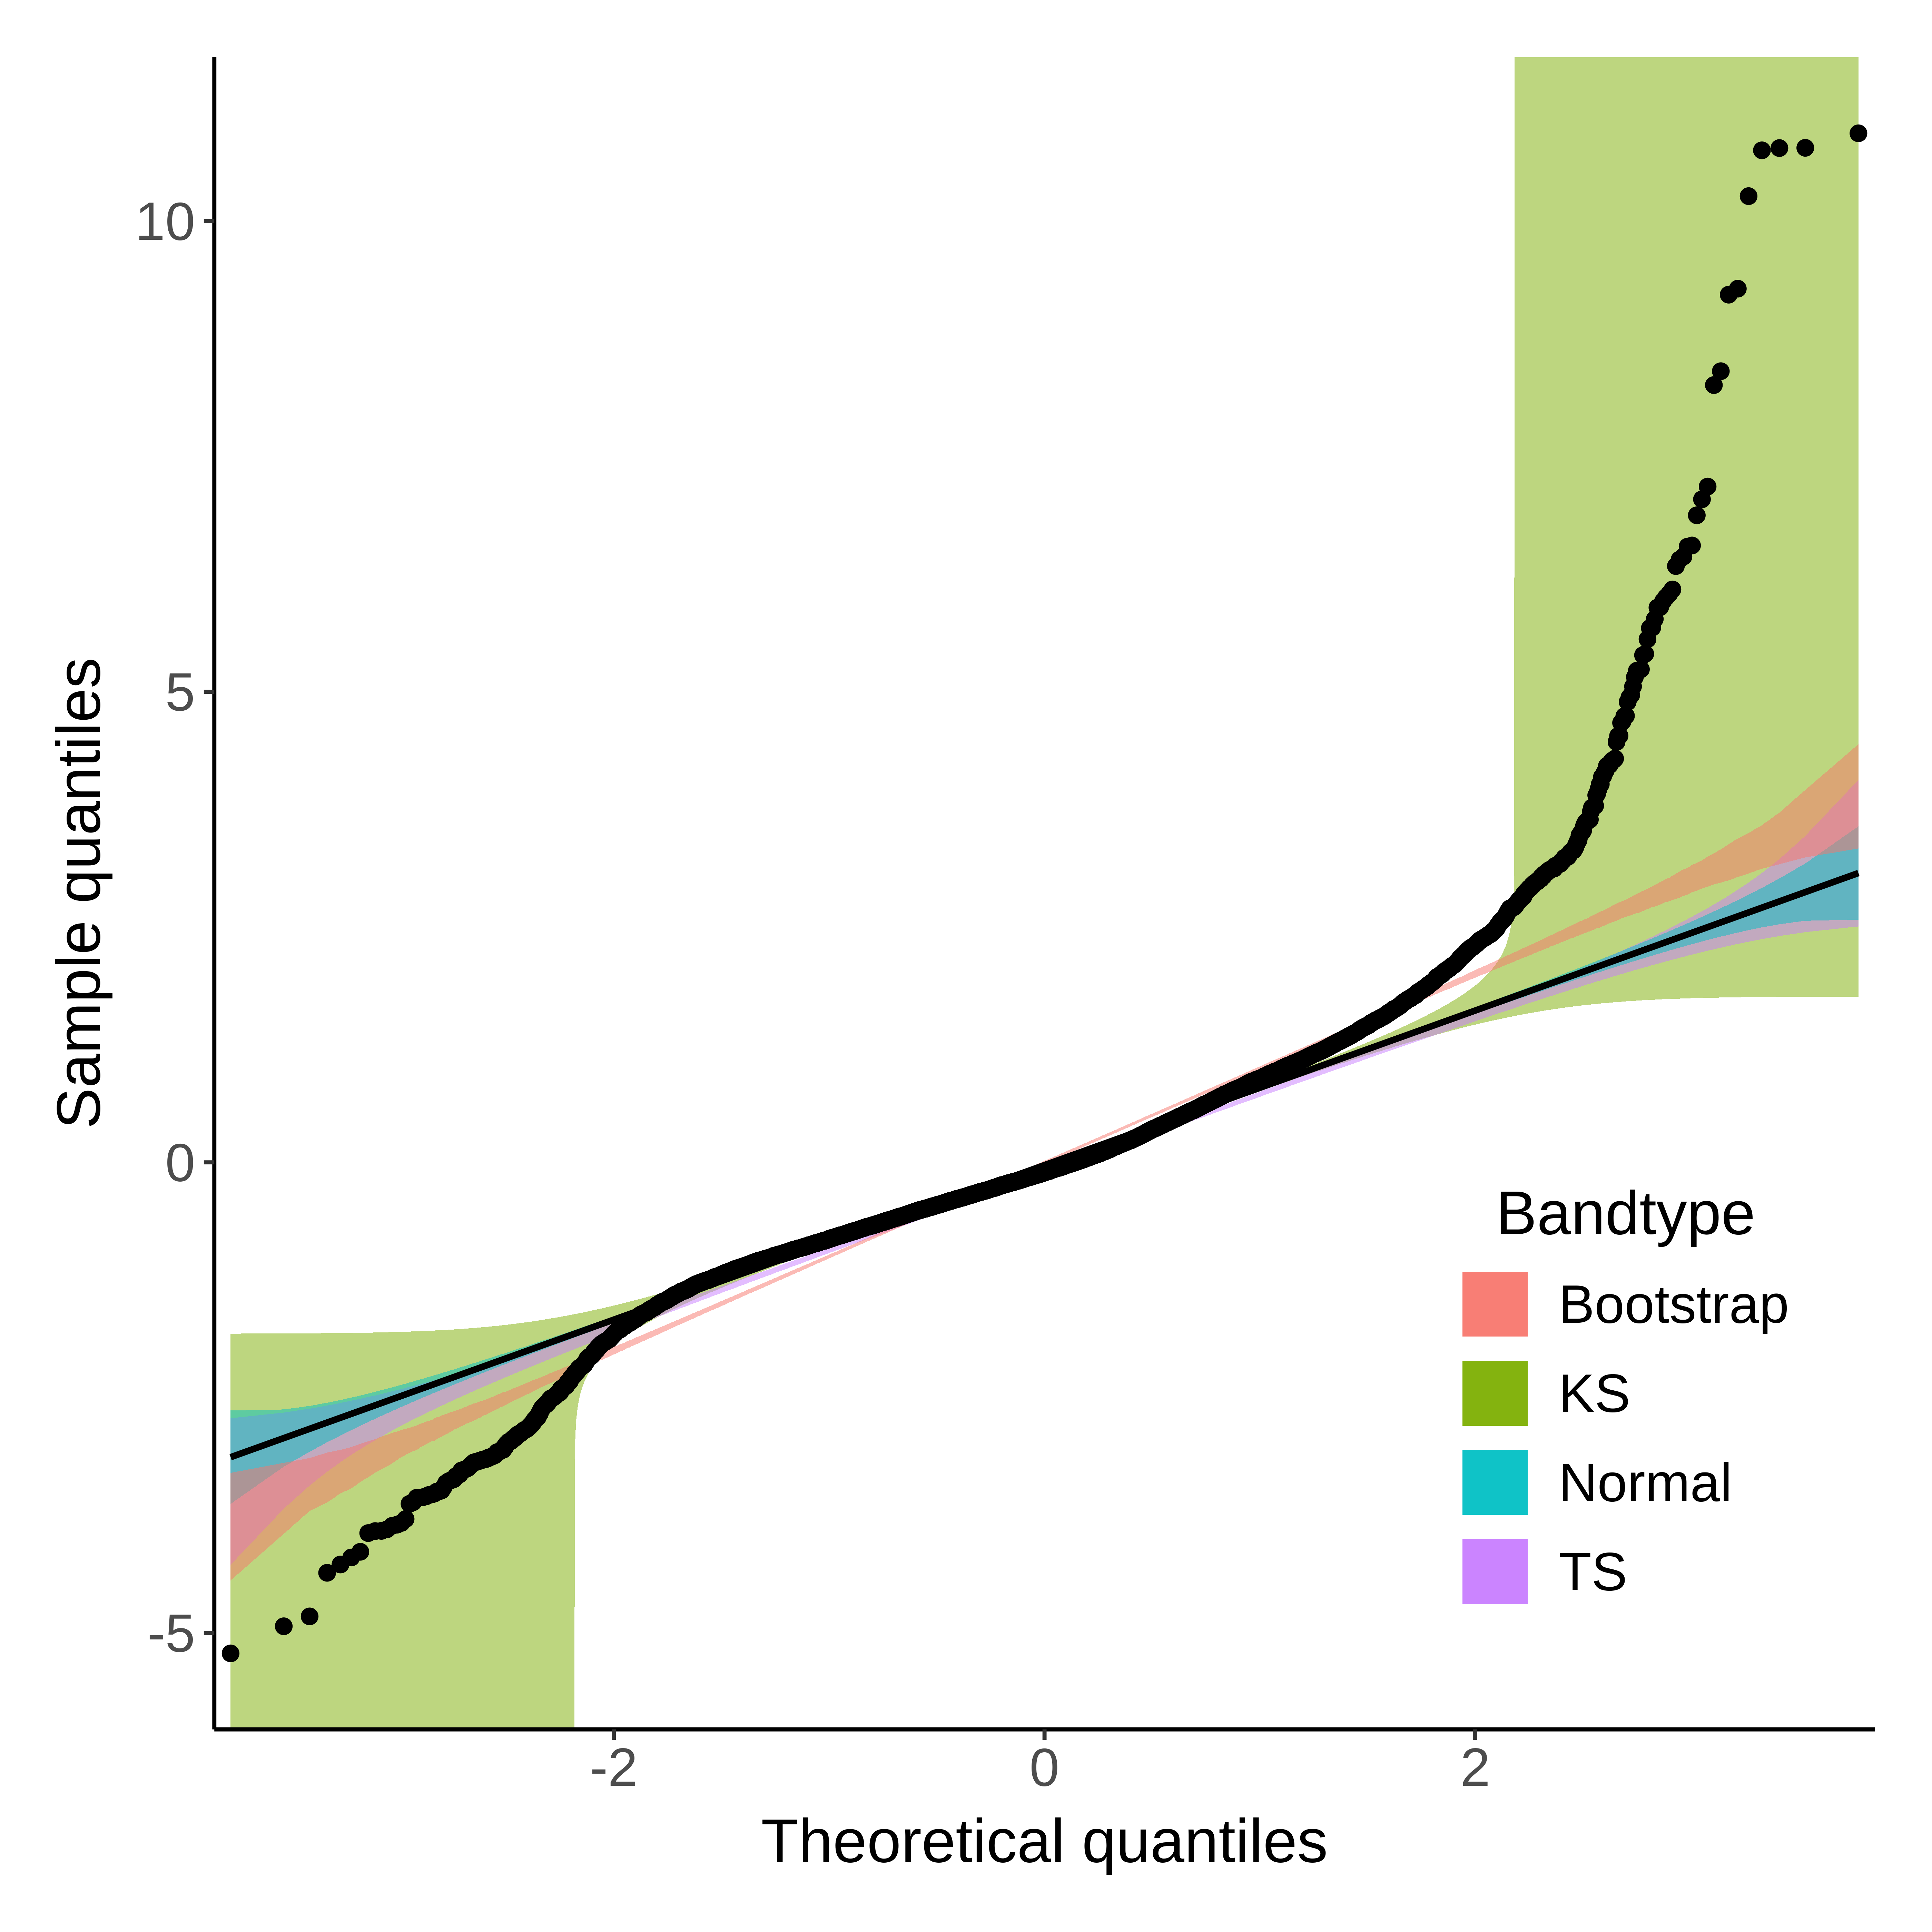
\includegraphics[width=0.65\linewidth]{/Users/pablodejuanbernabeu/Library/CloudStorage/OneDrive-LancasterUniversity/semanticpriming-semanticdecision-lexicaldecision/lexicaldecision/frequentist_analysis/model_diagnostics/plots/lexicaldecision_residuals} 

}

\caption{Residuals of the linear mixed-effects model from the lexical decision study. The outliers in the residuals deviate from the coloured areas indicating an acceptable normality. \linebreak KS = Kolmogorov-Smirnov test; TS = tail-sensitive confidence bands.}\label{fig:lexicaldecision-residuals}
\end{figure}

\clearpage

\renewcommand{\thefigure}{C\arabic{figure}} \setcounter{figure}{0}
\renewcommand{\thetable}{C\arabic{table}} \setcounter{table}{0}

\hypertarget{appendix-C-Bayesian-analysis-diagnostics}{%
\section{Appendix C: Diagnostics for the Bayesian analyses}\label{appendix-C-Bayesian-analysis-diagnostics}}

This appendix presents diagnostics for the Bayesian analyses. In each study, prior predictive checks are presented before posterior predictive checks. Furthermore, in each of these checks, the models presented first have the default Gaussian distribution, whereas the next series have an exponentially modified Gaussian (dubbed `ex-Gaussian') distribution with an identity link function (for details, see the section titled `Distributions and prior predictive checks' in the main article). Eyeball estimation is used to assess the outcomes of these checks (for background on predictive checks and for alternative estimation procedures, see Gelman et al., 1996; Moran et al., 2021; Schoot et al., 2021). One diagnostic not shown in this appendix is the \(\widehat R\), which is shown in \protect\hyperlink{appendix-E-Bayesian-analysis-results}{\underline{Appendix E}} instead.

\hypertarget{study1-bayesian-diagnostics}{%
\subsection{Study 1: Semantic priming}\label{study1-bayesian-diagnostics}}

\hypertarget{prior-predictive-checks}{%
\subsubsection{Prior predictive checks}\label{prior-predictive-checks}}

Figures \ref{fig:semanticpriming-priorpredictivecheck-informativepriors}, \ref{fig:semanticpriming-priorpredictivecheck-weaklyinformativepriors} and \ref{fig:semanticpriming-priorpredictivecheck-diffusepriors} show the prior predictive checks for the Gaussian models. These plots show the maximum, mean and minimum values of the observed data (\(y\)) and those of the predicted distribution (\(y_{rep}\), which stands for \emph{rep}lications of the outcome). The way of interpreting these plots is by comparing the observed data to the predicted distribution. The specifics of this vary across the three plots in the series. Firstly, in the upper plot, which shows the maximum values, the ideal scenario would have the observed (\(y\)) value overlapping with the maximum value of the predicted distribution (\(y_{rep}\)). Secondly, in the middle plot, showing the mean values, the ideal scenario would show the observed (\(y\)) value overlapping with the mean value of the predicted distribution (\(y_{rep}\)). Lastly, in the lower plot, which shows the minimum values, the ideal scenario would have the observed (\(y\)) value overlapping with the minimum value of the predicted distribution (\(y_{rep}\)). The overlap need not be absolute but the closer the observed and the predicted values on the X axis, the better. As such, the three predictive checks below---corresponding to models that used the default Gaussian distribution---show that the priors fitted the data acceptably but not very well.



\begin{figure}

{\centering 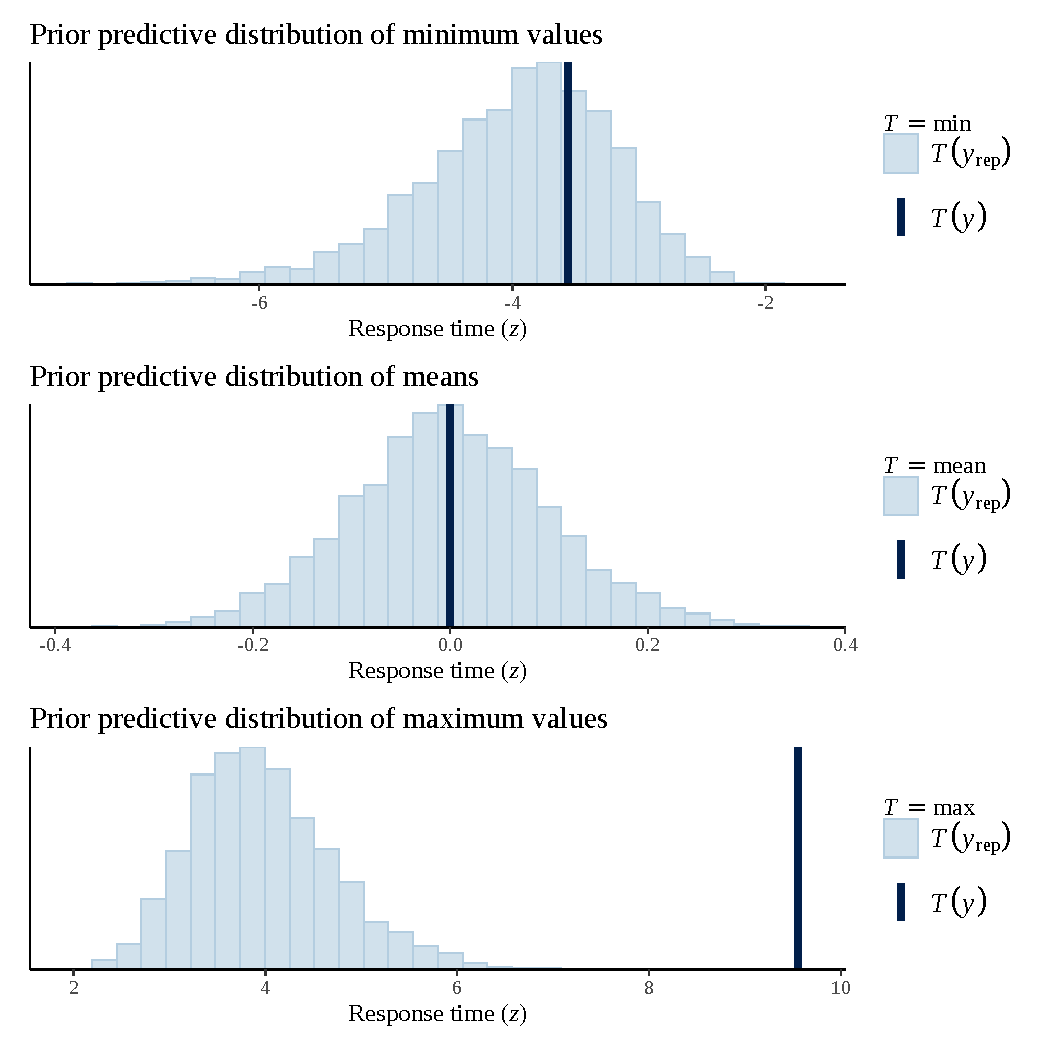
\includegraphics[width=0.8\linewidth]{/Users/pablodejuanbernabeu/Library/CloudStorage/OneDrive-LancasterUniversity/semanticpriming-semanticdecision-lexicaldecision/semanticpriming/bayesian_analysis/prior_predictive_checks/plots/semanticpriming_priorpredictivecheck_informativepriors} 

}

\caption{Prior predictive checks for the Gaussian, informative prior model from the semantic priming study. \(y\) = observed data; \(y_{rep}\) = predicted data.}\label{fig:semanticpriming-priorpredictivecheck-informativepriors}
\end{figure}



\begin{figure}

{\centering 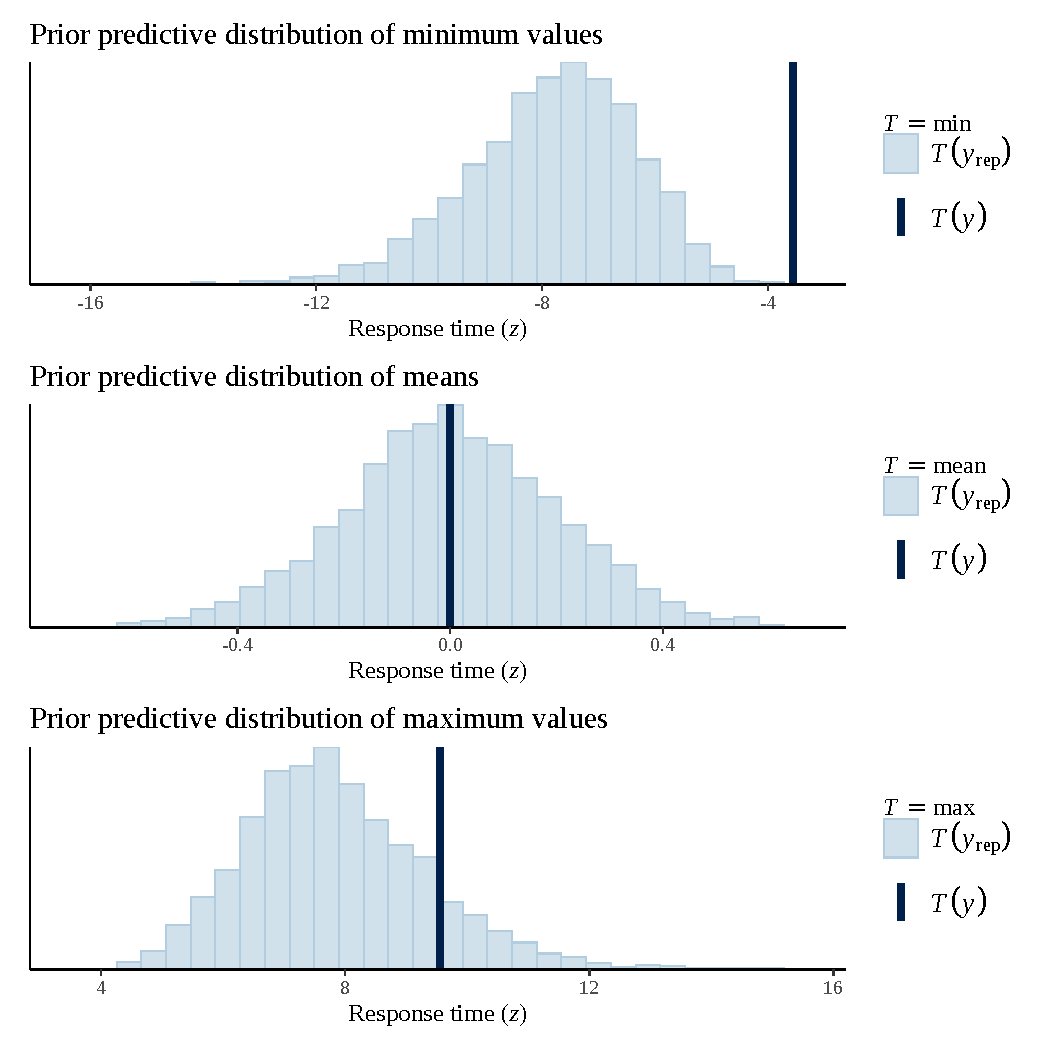
\includegraphics[width=0.8\linewidth]{/Users/pablodejuanbernabeu/Library/CloudStorage/OneDrive-LancasterUniversity/semanticpriming-semanticdecision-lexicaldecision/semanticpriming/bayesian_analysis/prior_predictive_checks/plots/semanticpriming_priorpredictivecheck_weaklyinformativepriors} 

}

\caption{Prior predictive checks for the Gaussian, weakly-informative prior model from the semantic priming study. \(y\) = observed data; \(y_{rep}\) = predicted data.}\label{fig:semanticpriming-priorpredictivecheck-weaklyinformativepriors}
\end{figure}



\begin{figure}

{\centering 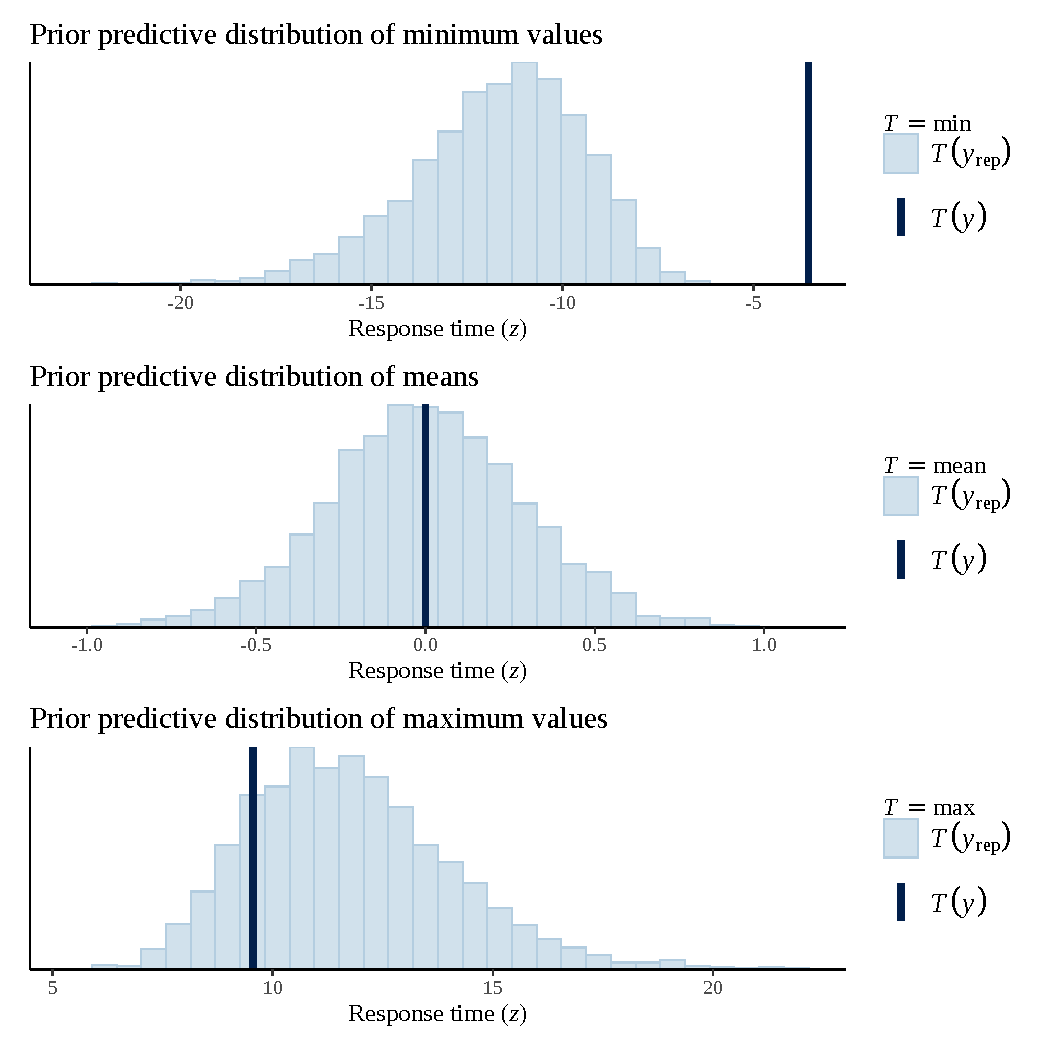
\includegraphics[width=0.8\linewidth]{/Users/pablodejuanbernabeu/Library/CloudStorage/OneDrive-LancasterUniversity/semanticpriming-semanticdecision-lexicaldecision/semanticpriming/bayesian_analysis/prior_predictive_checks/plots/semanticpriming_priorpredictivecheck_diffusepriors} 

}

\caption{Prior predictive checks for the Gaussian, diffuse prior model from the semantic priming study. \(y\) = observed data; \(y_{rep}\) = predicted data.}\label{fig:semanticpriming-priorpredictivecheck-diffusepriors}
\end{figure}

In contrast to the above results, Figures \ref{fig:semanticpriming-priorpredictivecheck-informativepriors-exgaussian}, \ref{fig:semanticpriming-priorpredictivecheck-weaklyinformativepriors-exgaussian} and \ref{fig:semanticpriming-priorpredictivecheck-diffusepriors-exgaussian} demonstrate that, when an ex-Gaussian distribution was used, the priors fitted the data far better, which converged with the results of a similar comparison performed by Rodríguez-Ferreiro et al. (2020) (see supplementary materials of the latter study).



\begin{figure}

{\centering 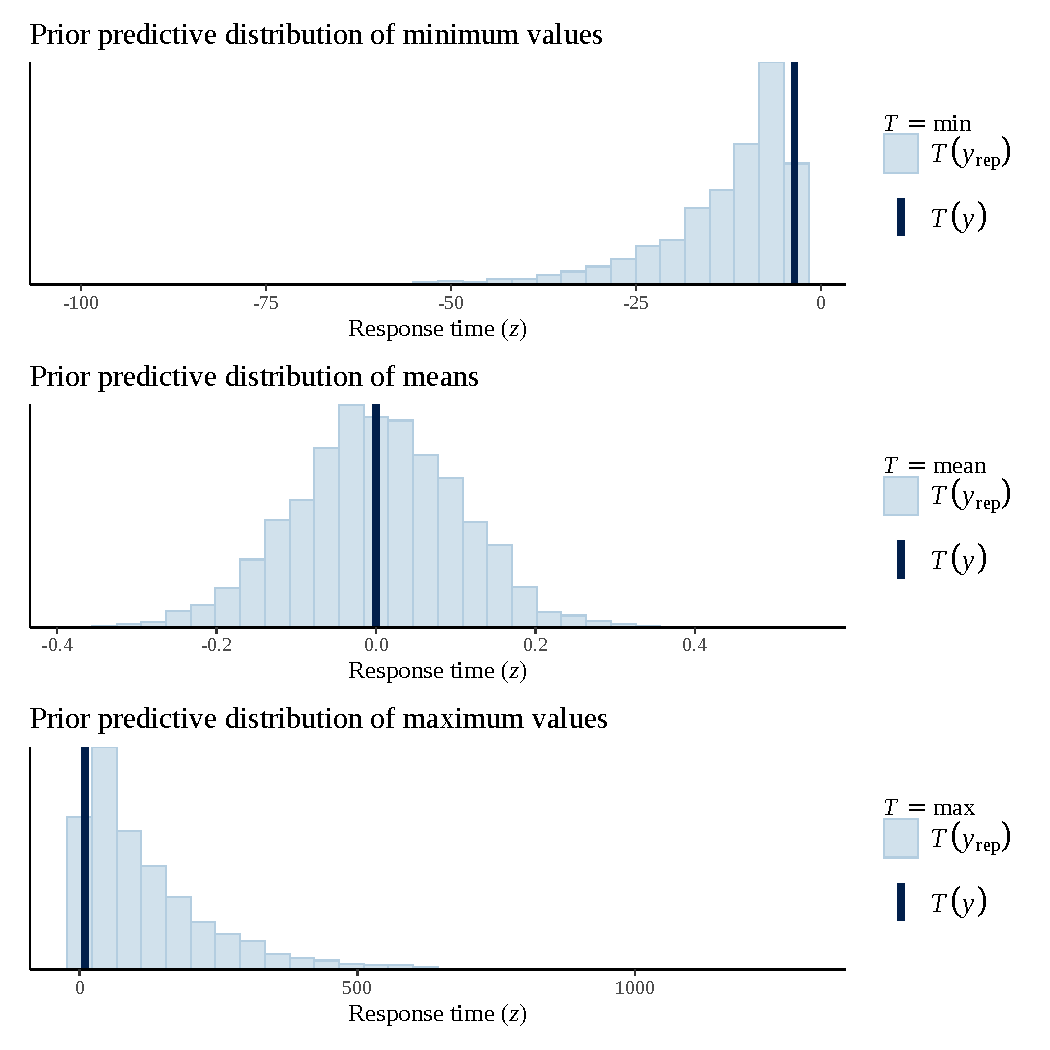
\includegraphics[width=0.8\linewidth]{/Users/pablodejuanbernabeu/Library/CloudStorage/OneDrive-LancasterUniversity/semanticpriming-semanticdecision-lexicaldecision/semanticpriming/bayesian_analysis/prior_predictive_checks/plots/semanticpriming_priorpredictivecheck_informativepriors_exgaussian} 

}

\caption{Prior predictive checks for the ex-Gaussian, informative prior model from the semantic priming study. \(y\) = observed data; \(y_{rep}\) = predicted data.}\label{fig:semanticpriming-priorpredictivecheck-informativepriors-exgaussian}
\end{figure}



\begin{figure}

{\centering 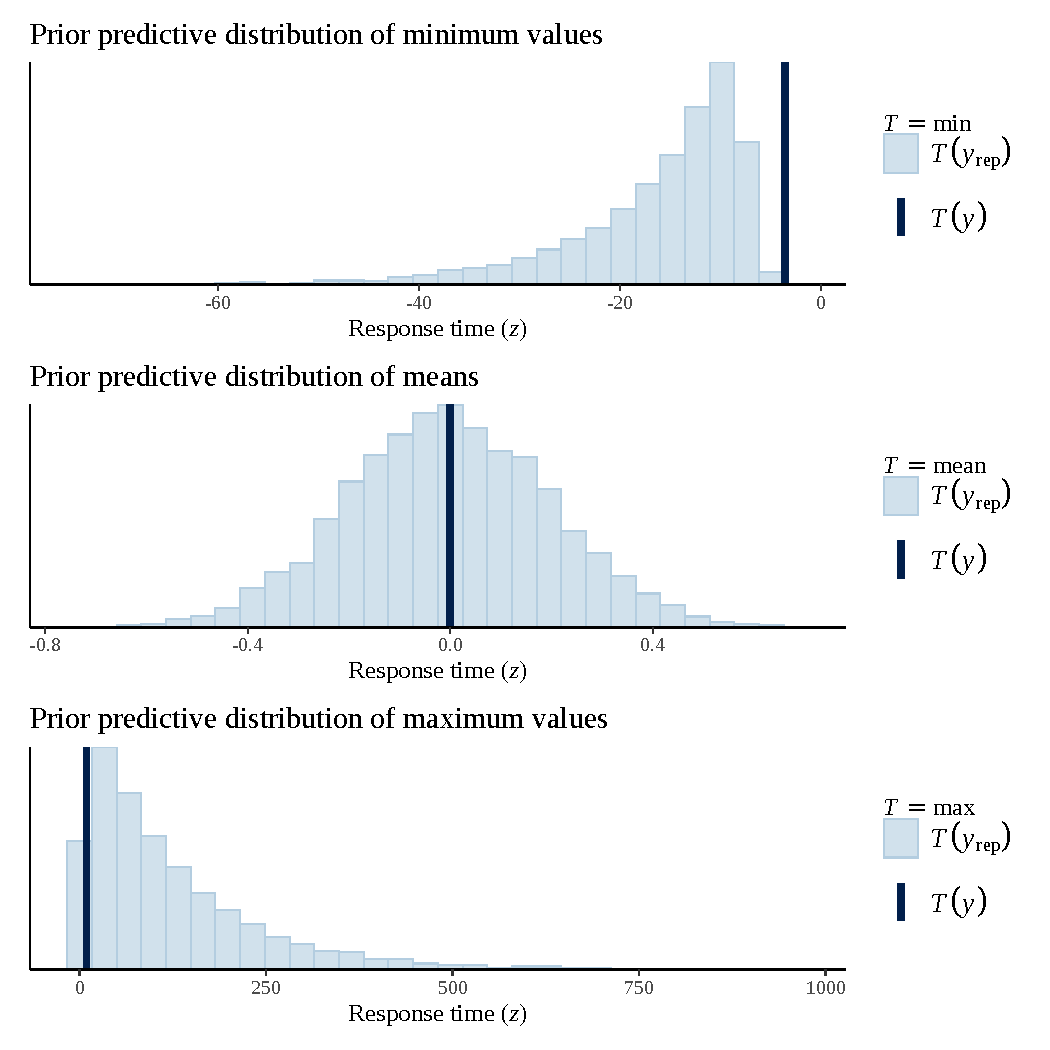
\includegraphics[width=0.8\linewidth]{/Users/pablodejuanbernabeu/Library/CloudStorage/OneDrive-LancasterUniversity/semanticpriming-semanticdecision-lexicaldecision/semanticpriming/bayesian_analysis/prior_predictive_checks/plots/semanticpriming_priorpredictivecheck_weaklyinformativepriors_exgaussian} 

}

\caption{Prior predictive checks for the ex-Gaussian, weakly-informative prior model from the semantic priming study. \(y\) = observed data; \(y_{rep}\) = predicted data.}\label{fig:semanticpriming-priorpredictivecheck-weaklyinformativepriors-exgaussian}
\end{figure}



\begin{figure}

{\centering 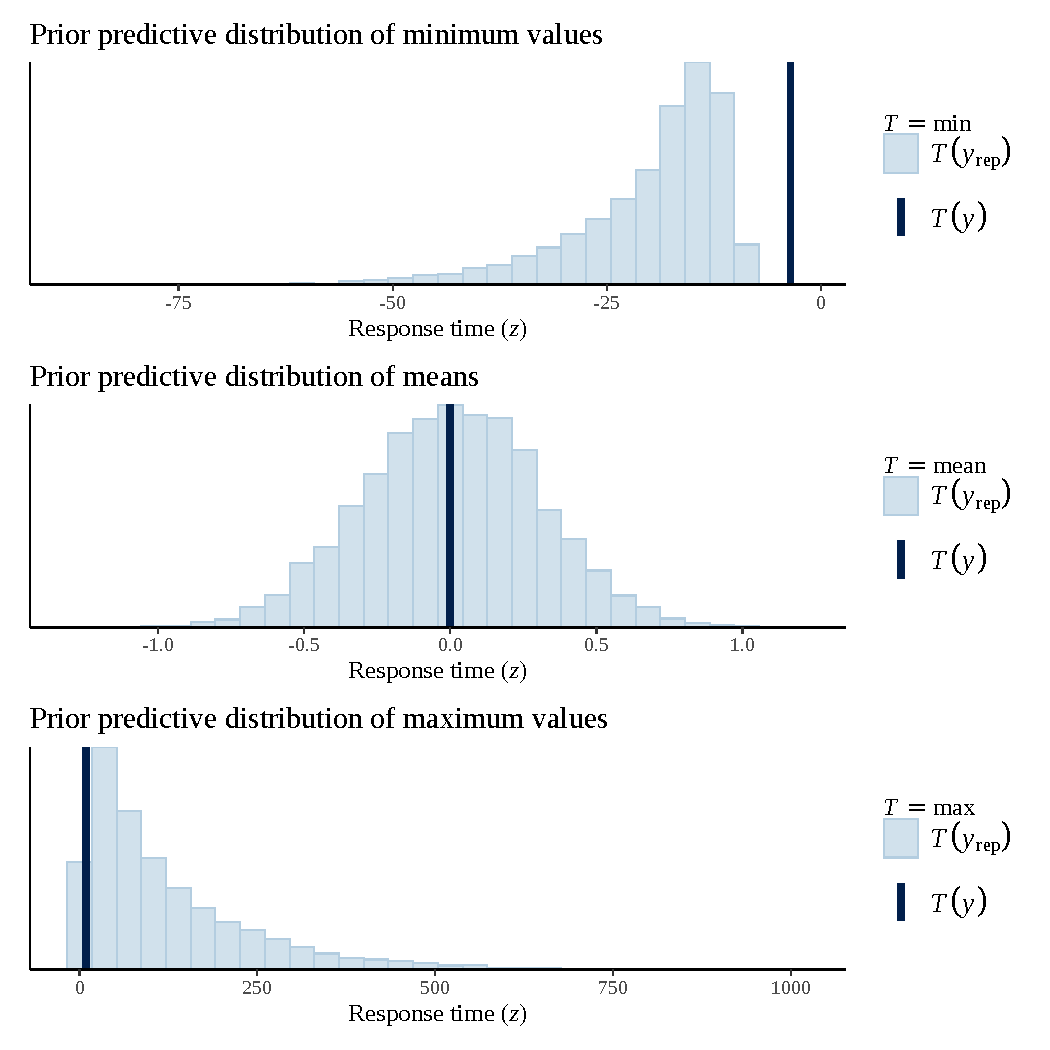
\includegraphics[width=0.8\linewidth]{/Users/pablodejuanbernabeu/Library/CloudStorage/OneDrive-LancasterUniversity/semanticpriming-semanticdecision-lexicaldecision/semanticpriming/bayesian_analysis/prior_predictive_checks/plots/semanticpriming_priorpredictivecheck_diffusepriors_exgaussian} 

}

\caption{Prior predictive checks for the ex-Gaussian, diffuse prior model from the semantic priming study. \(y\) = observed data; \(y_{rep}\) = predicted data.}\label{fig:semanticpriming-priorpredictivecheck-diffusepriors-exgaussian}
\end{figure}

\hypertarget{posterior-predictive-checks}{%
\subsubsection{Posterior predictive checks}\label{posterior-predictive-checks}}

Based on the above results, the ex-Gaussian distribution was used in the final models. Figure \ref{fig:semanticpriming-posteriorpredictivechecks-allpriors-exgaussian} presents the posterior predictive checks the latter models. The interpretation of these plots is simple: the distributions of the observed (\(y\)) and the predicted data (\(y_{rep}\)) should be as similar as possible. As such, the plots below suggest that the results are trustworthy.



\begin{figure}

{\centering 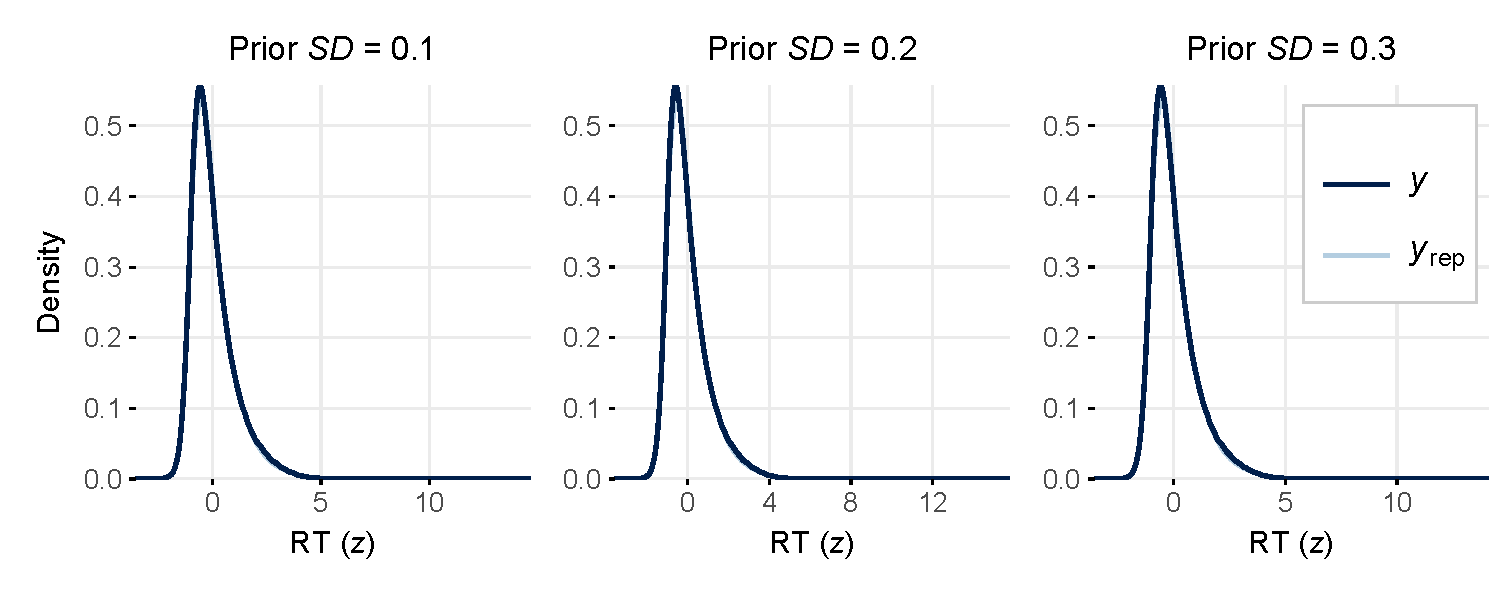
\includegraphics[width=1\linewidth]{/Users/pablodejuanbernabeu/Library/CloudStorage/OneDrive-LancasterUniversity/semanticpriming-semanticdecision-lexicaldecision/semanticpriming/bayesian_analysis/posterior_predictive_checks/plots/semanticpriming_posteriorpredictivechecks_allpriors_exgaussian} 

}

\caption{Posterior predictive checks for the (ex-Gaussian) models from the semantic priming study. \(y\) = observed data; \(y_{rep}\) = predicted data.}\label{fig:semanticpriming-posteriorpredictivechecks-allpriors-exgaussian}
\end{figure}

\hypertarget{study-2-semantic-decision-3}{%
\subsection{Study 2: Semantic decision}\label{study-2-semantic-decision-3}}

\hypertarget{prior-predictive-checks-1}{%
\subsubsection{Prior predictive checks}\label{prior-predictive-checks-1}}

Figures \ref{fig:semanticdecision-priorpredictivecheck-informativepriors}, \ref{fig:semanticdecision-priorpredictivecheck-weaklyinformativepriors} and \ref{fig:semanticdecision-priorpredictivecheck-diffusepriors} show the prior predictive checks for the Gaussian models (for background on these checks, see \protect\hyperlink{study1-bayesian-diagnostics}{\underline{Study 1 above}}). The three plots---corresponding to models that used the default Gaussian distribution---show that the priors fitted the data acceptably but not very well.



\begin{figure}

{\centering 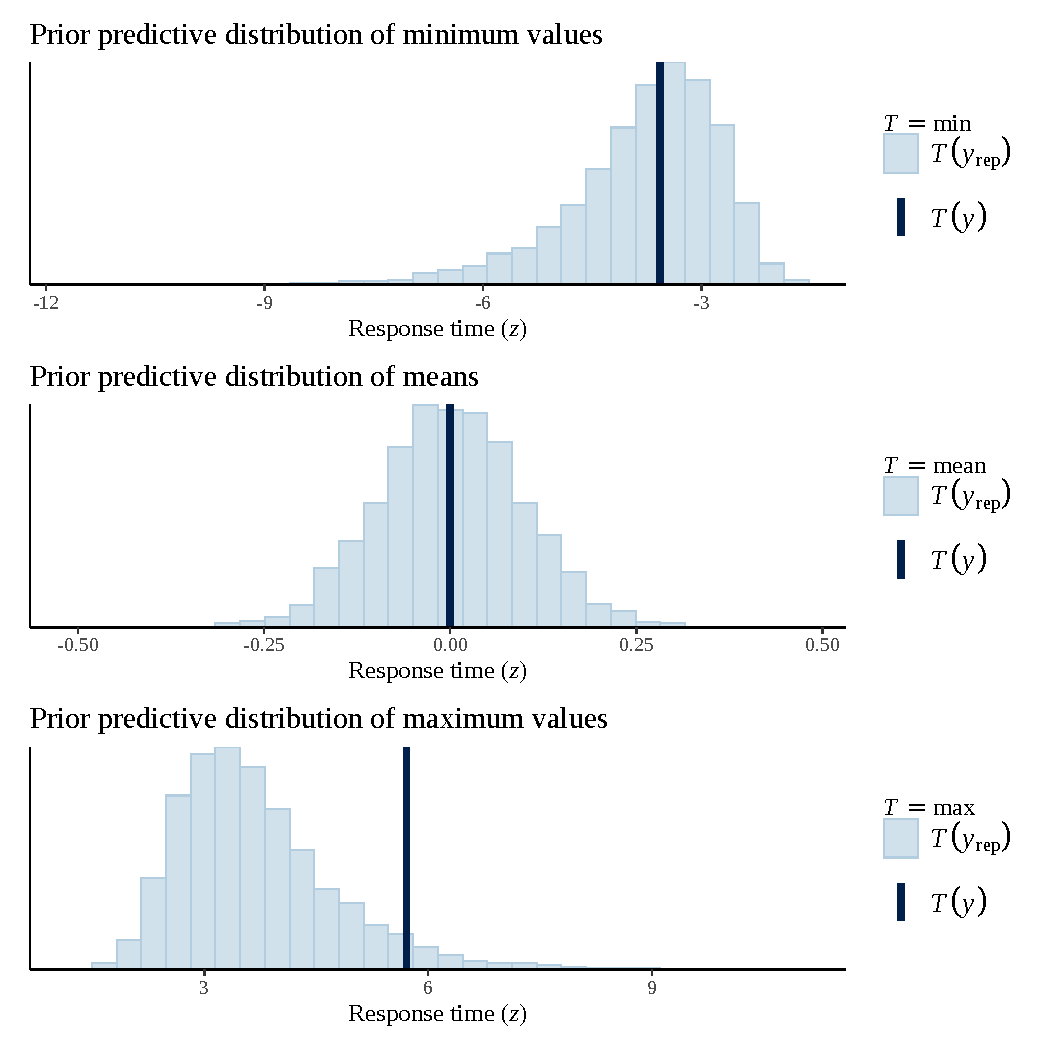
\includegraphics[width=0.8\linewidth]{/Users/pablodejuanbernabeu/Library/CloudStorage/OneDrive-LancasterUniversity/semanticpriming-semanticdecision-lexicaldecision/semanticdecision/bayesian_analysis/prior_predictive_checks/plots/semanticdecision_priorpredictivecheck_informativepriors} 

}

\caption{Prior predictive checks for the Gaussian, informative prior model from the semantic decision study. \(y\) = observed data; \(y_{rep}\) = predicted data.}\label{fig:semanticdecision-priorpredictivecheck-informativepriors}
\end{figure}



\begin{figure}

{\centering 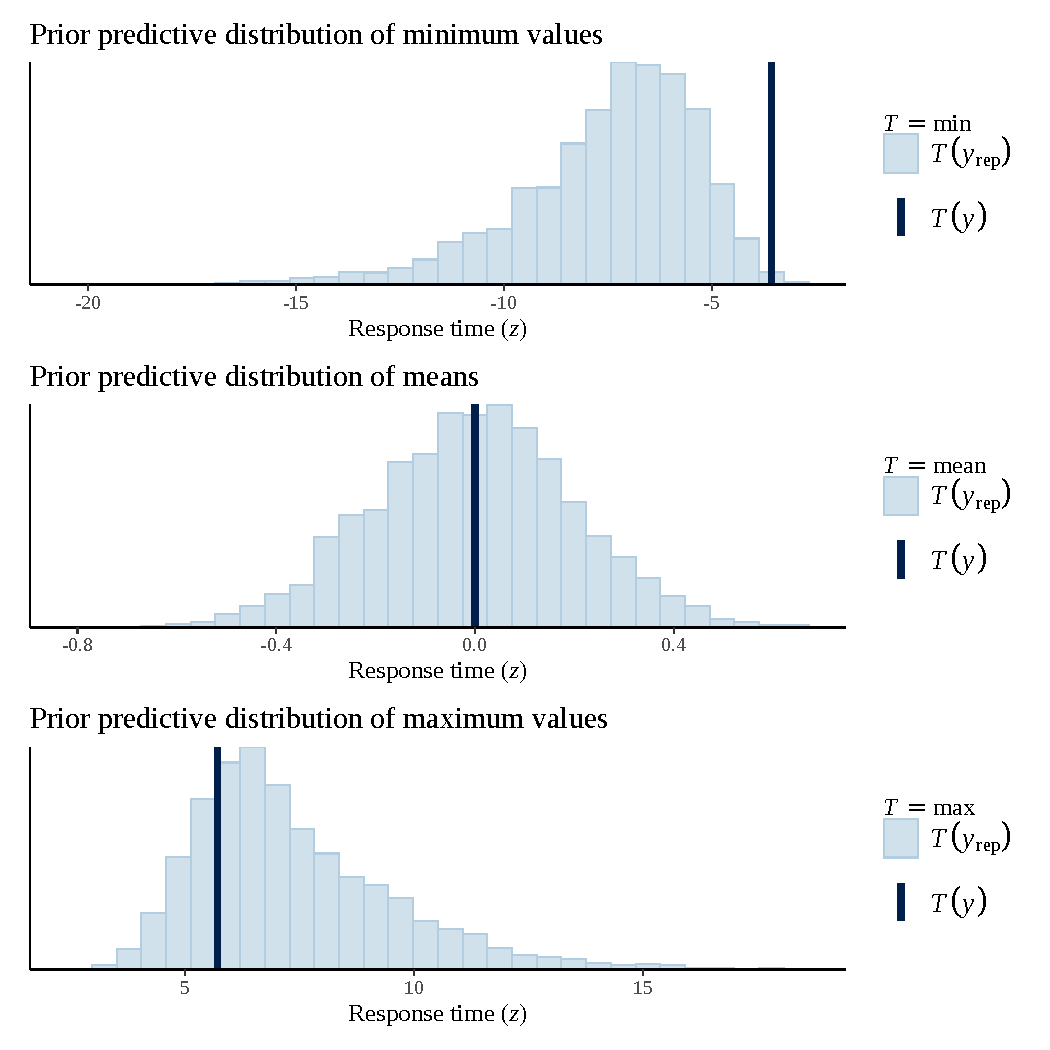
\includegraphics[width=0.8\linewidth]{/Users/pablodejuanbernabeu/Library/CloudStorage/OneDrive-LancasterUniversity/semanticpriming-semanticdecision-lexicaldecision/semanticdecision/bayesian_analysis/prior_predictive_checks/plots/semanticdecision_priorpredictivecheck_weaklyinformativepriors} 

}

\caption{Prior predictive checks for the Gaussian, weakly-informative prior model from the semantic decision study. \(y\) = observed data; \(y_{rep}\) = predicted data.}\label{fig:semanticdecision-priorpredictivecheck-weaklyinformativepriors}
\end{figure}



\begin{figure}

{\centering 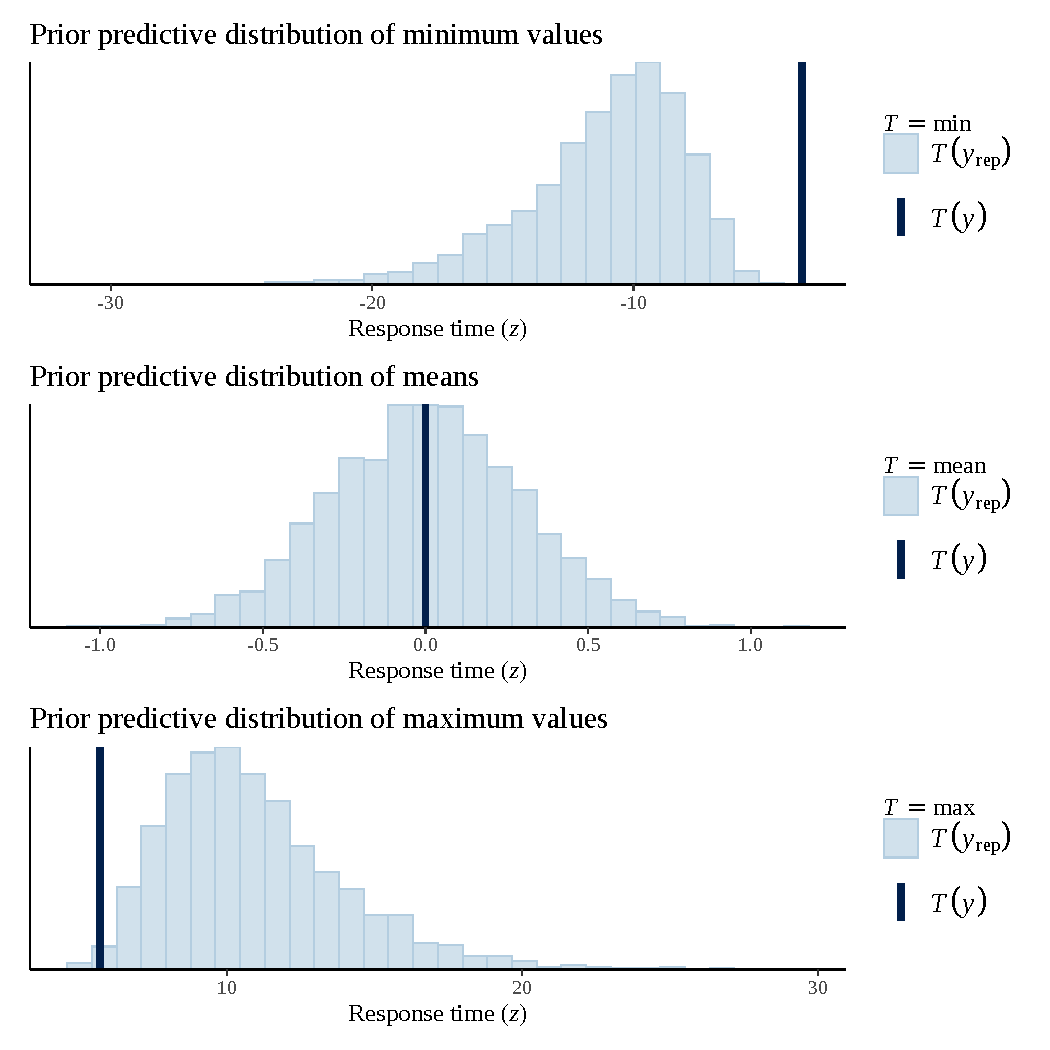
\includegraphics[width=0.8\linewidth]{/Users/pablodejuanbernabeu/Library/CloudStorage/OneDrive-LancasterUniversity/semanticpriming-semanticdecision-lexicaldecision/semanticdecision/bayesian_analysis/prior_predictive_checks/plots/semanticdecision_priorpredictivecheck_diffusepriors} 

}

\caption{Prior predictive checks for the Gaussian, diffuse prior model from the semantic decision study. \(y\) = observed data; \(y_{rep}\) = predicted data.}\label{fig:semanticdecision-priorpredictivecheck-diffusepriors}
\end{figure}

In contrast to the results from the Gaussian models, Figures \ref{fig:semanticdecision-priorpredictivecheck-informativepriors-exgaussian}, \ref{fig:semanticdecision-priorpredictivecheck-weaklyinformativepriors-exgaussian} and \ref{fig:semanticdecision-priorpredictivecheck-diffusepriors-exgaussian} demonstrate that, when an ex-Gaussian distribution was used, the priors fitted the data far better, which converged with the results found in Study 1.



\begin{figure}

{\centering 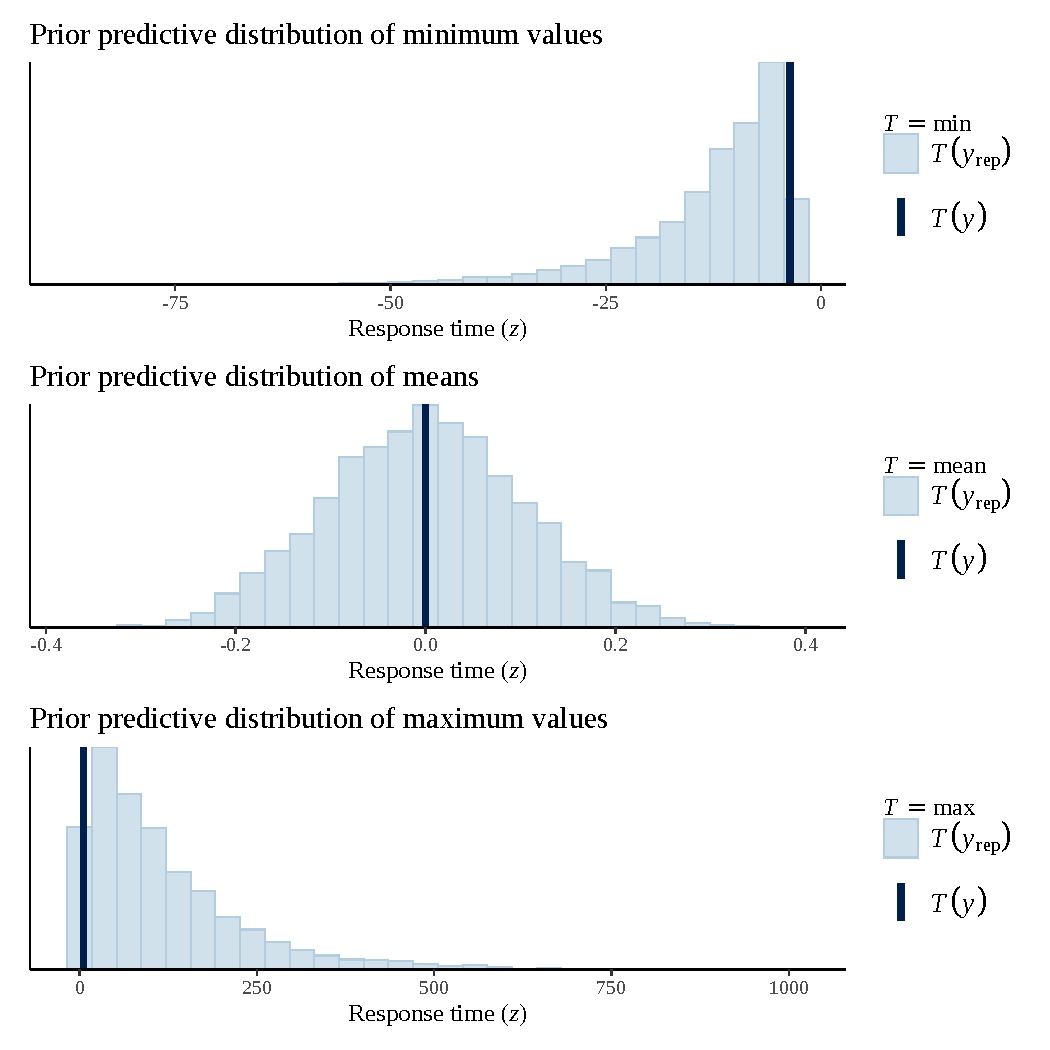
\includegraphics[width=0.8\linewidth]{/Users/pablodejuanbernabeu/Library/CloudStorage/OneDrive-LancasterUniversity/semanticpriming-semanticdecision-lexicaldecision/semanticdecision/bayesian_analysis/prior_predictive_checks/plots/semanticdecision_priorpredictivecheck_informativepriors_exgaussian} 

}

\caption{Prior predictive checks for the ex-Gaussian, informative prior model from the semantic decision study. \(y\) = observed data; \(y_{rep}\) = predicted data.}\label{fig:semanticdecision-priorpredictivecheck-informativepriors-exgaussian}
\end{figure}



\begin{figure}

{\centering 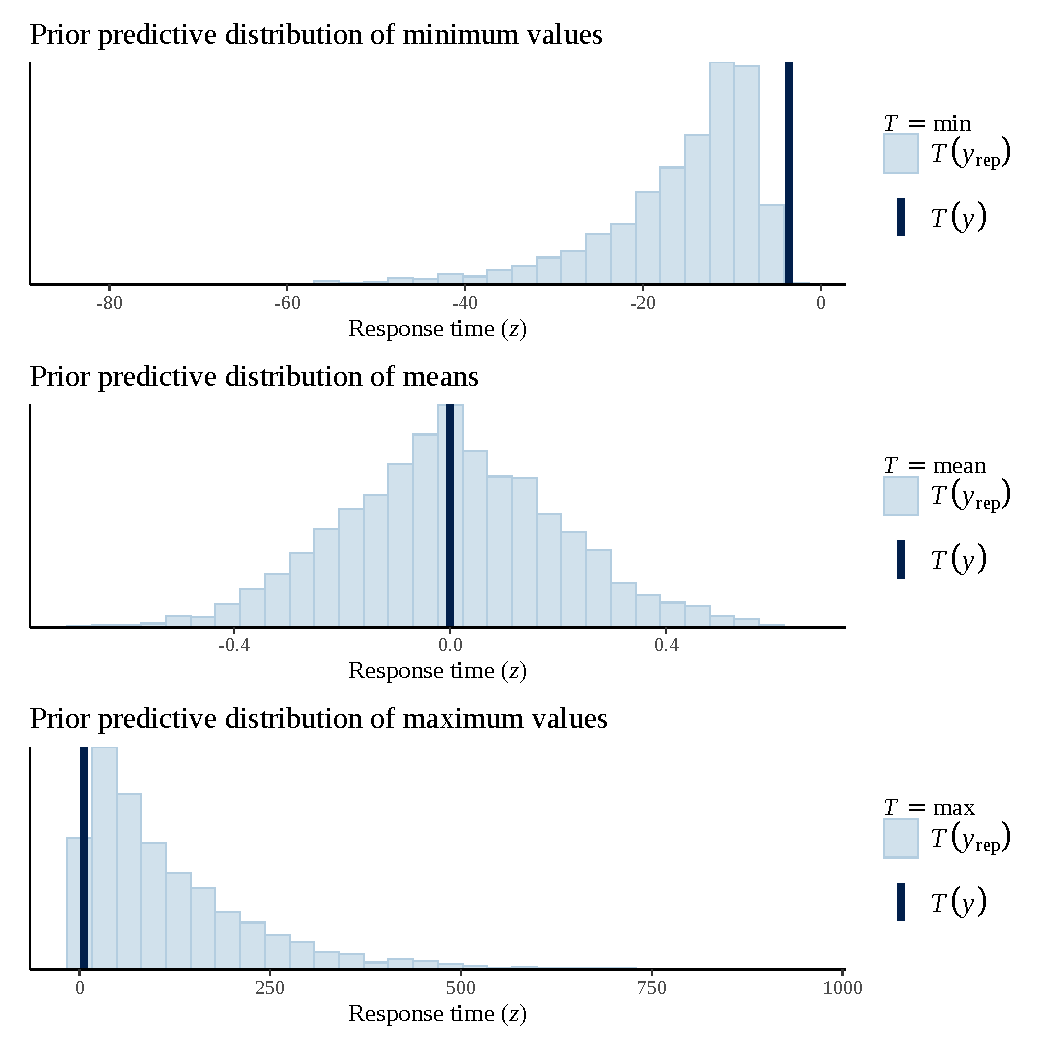
\includegraphics[width=0.8\linewidth]{/Users/pablodejuanbernabeu/Library/CloudStorage/OneDrive-LancasterUniversity/semanticpriming-semanticdecision-lexicaldecision/semanticdecision/bayesian_analysis/prior_predictive_checks/plots/semanticdecision_priorpredictivecheck_weaklyinformativepriors_exgaussian} 

}

\caption{Prior predictive checks for the ex-Gaussian, weakly-informative prior model from the semantic decision study. \(y\) = observed data; \(y_{rep}\) = predicted data.}\label{fig:semanticdecision-priorpredictivecheck-weaklyinformativepriors-exgaussian}
\end{figure}



\begin{figure}

{\centering 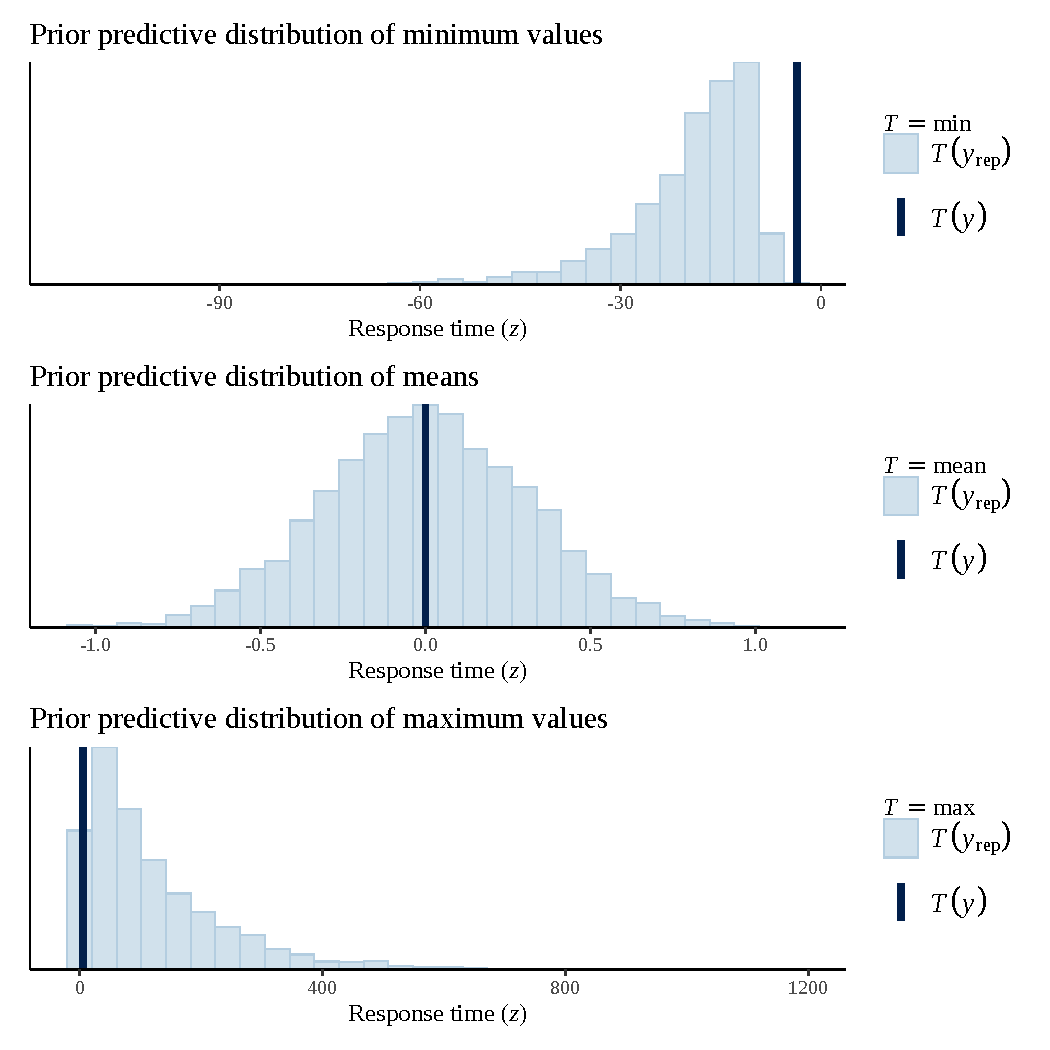
\includegraphics[width=0.8\linewidth]{/Users/pablodejuanbernabeu/Library/CloudStorage/OneDrive-LancasterUniversity/semanticpriming-semanticdecision-lexicaldecision/semanticdecision/bayesian_analysis/prior_predictive_checks/plots/semanticdecision_priorpredictivecheck_diffusepriors_exgaussian} 

}

\caption{Prior predictive checks for the ex-Gaussian, diffuse prior model from the semantic decision study. \(y\) = observed data; \(y_{rep}\) = predicted data.}\label{fig:semanticdecision-priorpredictivecheck-diffusepriors-exgaussian}
\end{figure}

\hypertarget{posterior-predictive-checks-1}{%
\subsubsection{Posterior predictive checks}\label{posterior-predictive-checks-1}}

Based on the above results, the ex-Gaussian distribution was used in the final models. Figure \ref{fig:semanticdecision-posteriorpredictivechecks-allpriors-exgaussian} presents the posterior predictive checks for the latter models. The interpretation of these plots is simple: the distributions of the observed (\(y\)) and the predicted data (\(y_{rep}\)) should be as similar as possible. As such, the plots below suggest that the results are not entirely trustworthy. Indeed, the results themselves (\protect\hyperlink{appendix-E-Bayesian-analysis-results}{\underline{Appendix E}}) are clearly not valid.



\begin{figure}

{\centering 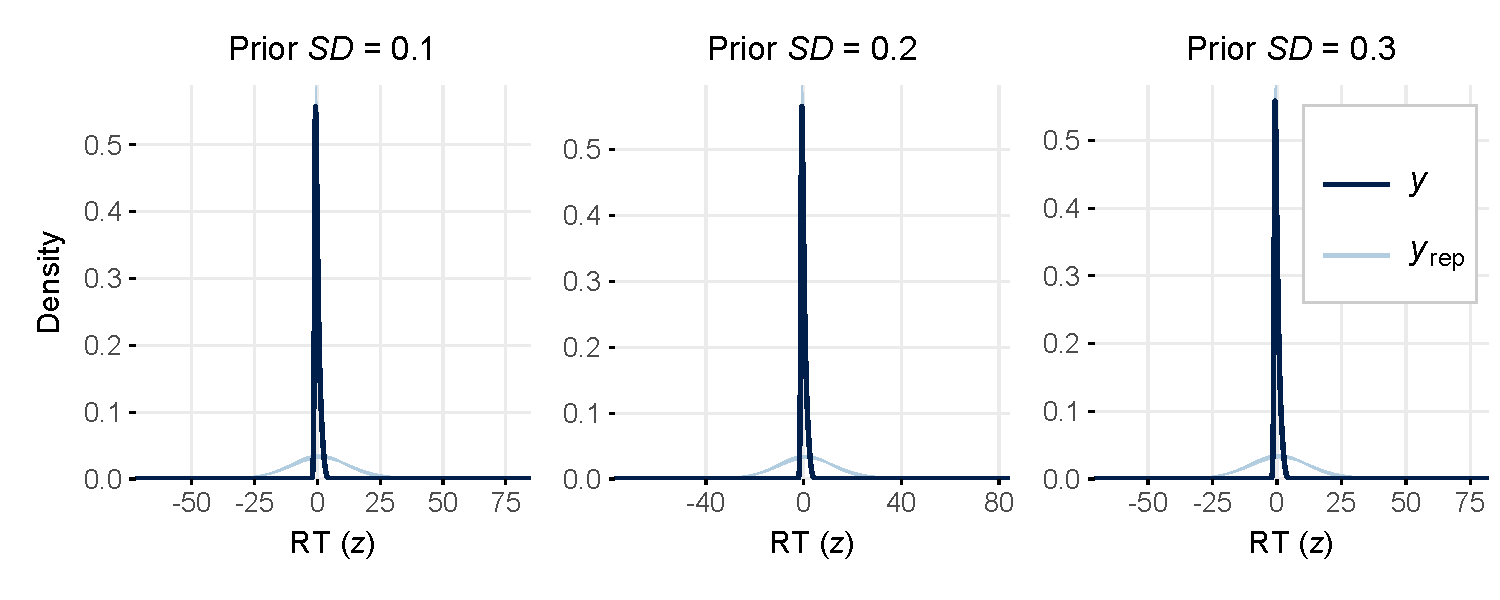
\includegraphics[width=1\linewidth]{/Users/pablodejuanbernabeu/Library/CloudStorage/OneDrive-LancasterUniversity/semanticpriming-semanticdecision-lexicaldecision/semanticdecision/bayesian_analysis/posterior_predictive_checks/plots/semanticdecision_posteriorpredictivechecks_allpriors_exgaussian} 

}

\caption{Posterior predictive checks for the (ex-Gaussian) models from the semantic decision study. \(y\) = observed data; \(y_{rep}\) = predicted data.}\label{fig:semanticdecision-posteriorpredictivechecks-allpriors-exgaussian}
\end{figure}

\hypertarget{study-3-lexical-decision-3}{%
\subsection{Study 3: Lexical decision}\label{study-3-lexical-decision-3}}

\hypertarget{prior-predictive-checks-2}{%
\subsubsection{Prior predictive checks}\label{prior-predictive-checks-2}}

Figures \ref{fig:lexicaldecision-priorpredictivecheck-informativepriors}, \ref{fig:lexicaldecision-priorpredictivecheck-weaklyinformativepriors} and \ref{fig:lexicaldecision-priorpredictivecheck-diffusepriors} show the prior predictive checks for the Gaussian models (for background on these checks, see \protect\hyperlink{study1-bayesian-diagnostics}{\underline{Study 1 above}}). The three plots---corresponding to models that used the default Gaussian distribution---show that the priors fitted the data acceptably but not very well.



\begin{figure}

{\centering 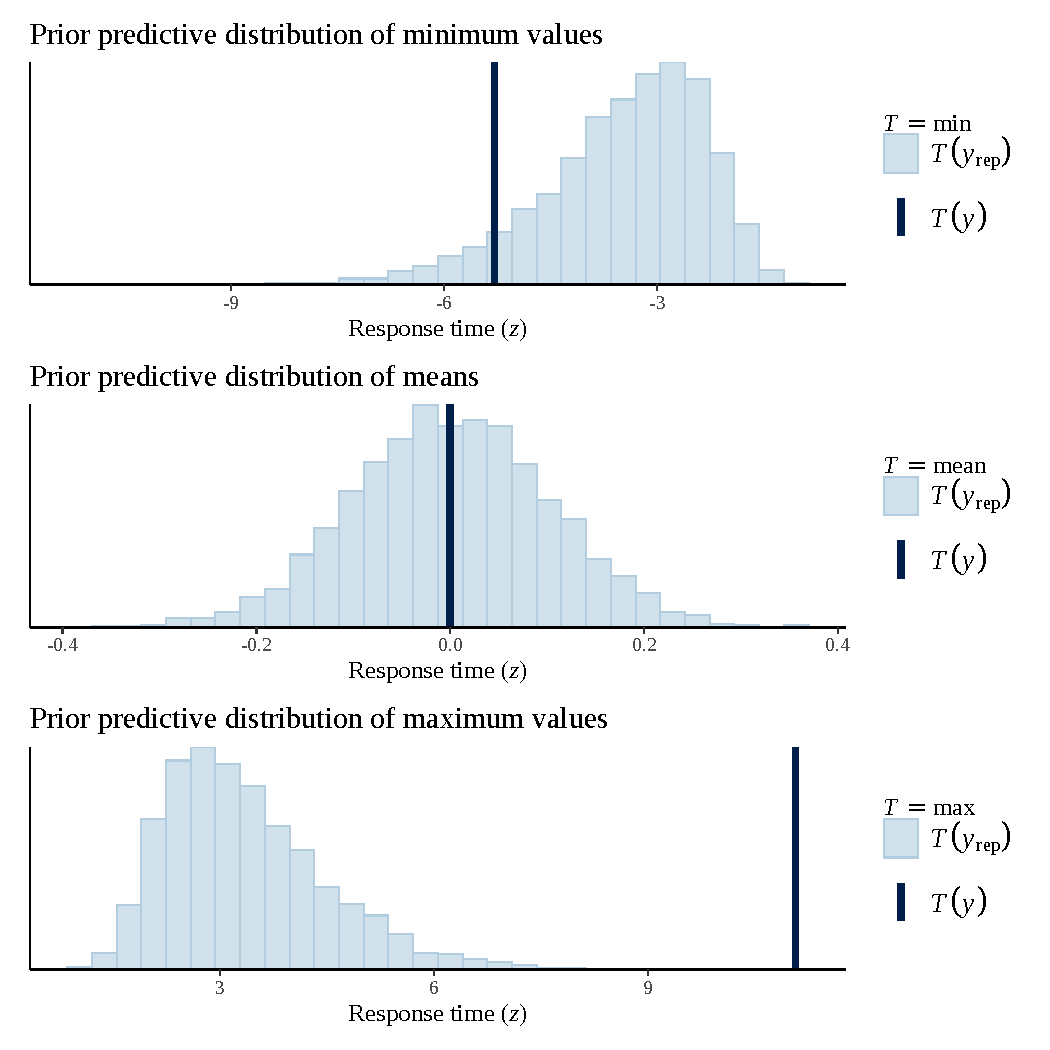
\includegraphics[width=0.8\linewidth]{/Users/pablodejuanbernabeu/Library/CloudStorage/OneDrive-LancasterUniversity/semanticpriming-semanticdecision-lexicaldecision/lexicaldecision/bayesian_analysis/prior_predictive_checks/plots/lexicaldecision_priorpredictivecheck_informativepriors} 

}

\caption{Prior predictive checks for the Gaussian, informative prior model from the lexical decision study. \(y\) = observed data; \(y_{rep}\) = predicted data.}\label{fig:lexicaldecision-priorpredictivecheck-informativepriors}
\end{figure}



\begin{figure}

{\centering 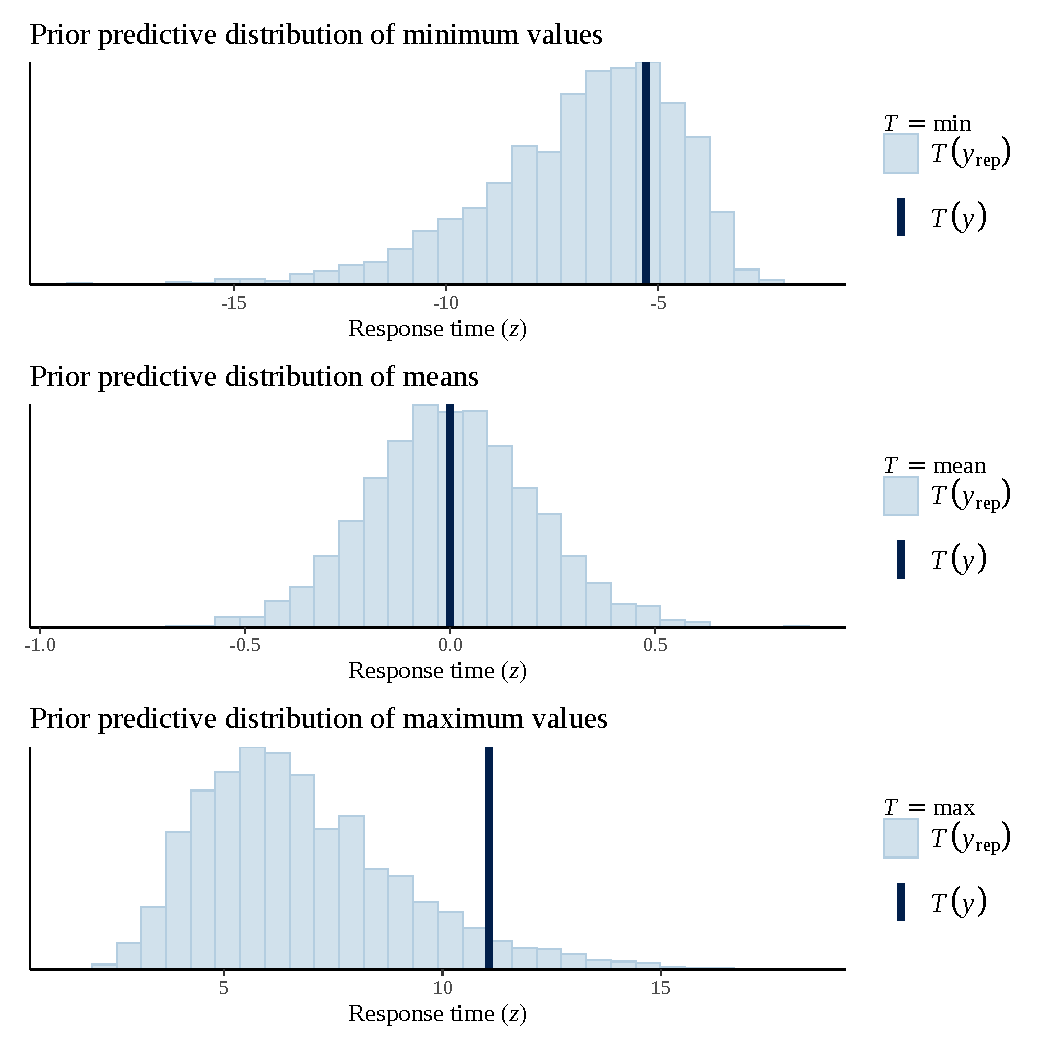
\includegraphics[width=0.8\linewidth]{/Users/pablodejuanbernabeu/Library/CloudStorage/OneDrive-LancasterUniversity/semanticpriming-semanticdecision-lexicaldecision/lexicaldecision/bayesian_analysis/prior_predictive_checks/plots/lexicaldecision_priorpredictivecheck_weaklyinformativepriors} 

}

\caption{Prior predictive checks for the Gaussian, weakly-informative prior model from the lexical decision study. \(y\) = observed data; \(y_{rep}\) = predicted data.}\label{fig:lexicaldecision-priorpredictivecheck-weaklyinformativepriors}
\end{figure}



\begin{figure}

{\centering 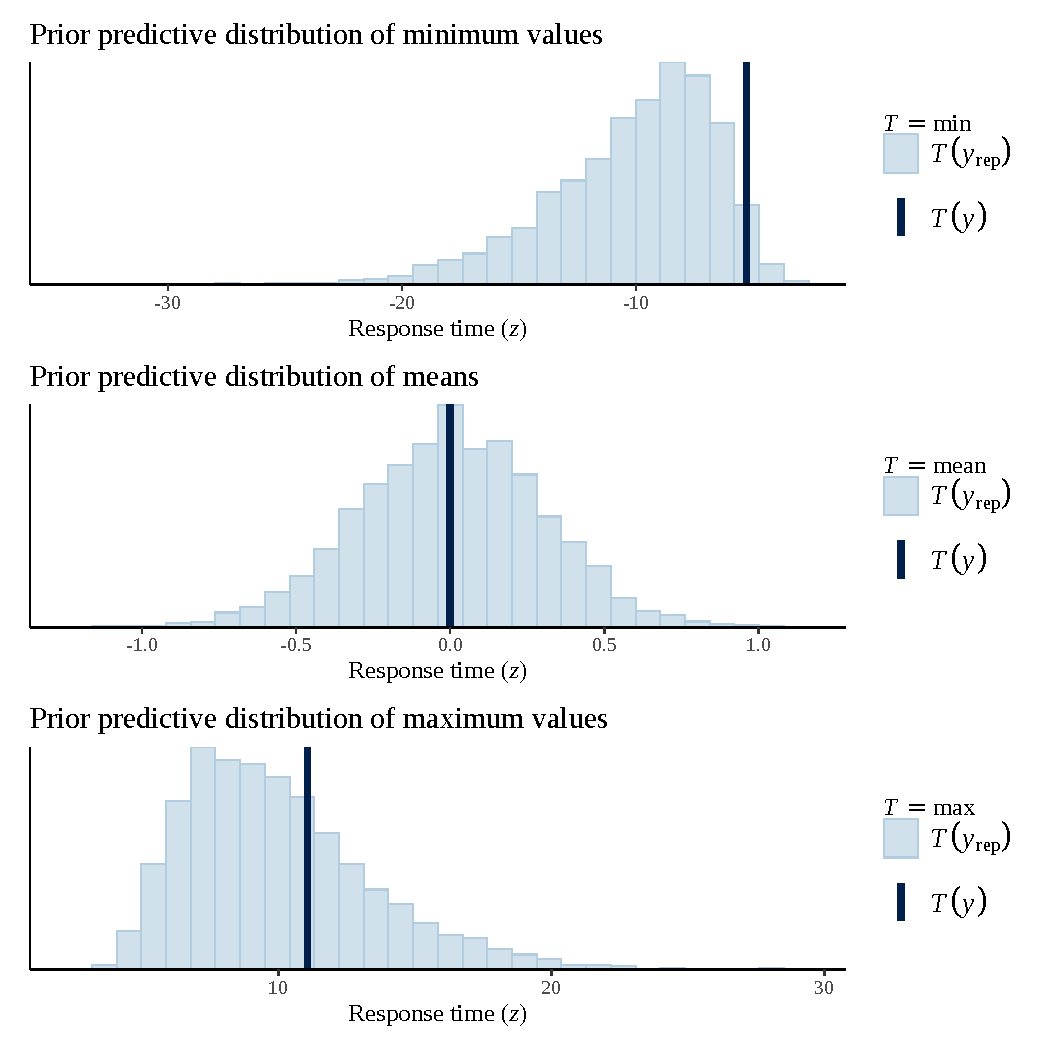
\includegraphics[width=0.8\linewidth]{/Users/pablodejuanbernabeu/Library/CloudStorage/OneDrive-LancasterUniversity/semanticpriming-semanticdecision-lexicaldecision/lexicaldecision/bayesian_analysis/prior_predictive_checks/plots/lexicaldecision_priorpredictivecheck_diffusepriors} 

}

\caption{Prior predictive checks for the Gaussian, diffuse prior model from the lexical decision study. \(y\) = observed data; \(y_{rep}\) = predicted data.}\label{fig:lexicaldecision-priorpredictivecheck-diffusepriors}
\end{figure}

In contrast to the results from the Gaussian models, Figures \ref{fig:lexicaldecision-priorpredictivecheck-informativepriors-exgaussian}, \ref{fig:lexicaldecision-priorpredictivecheck-weaklyinformativepriors-exgaussian} and \ref{fig:lexicaldecision-priorpredictivecheck-diffusepriors-exgaussian} demonstrate that, when an ex-Gaussian distribution was used, the priors fitted the data far better, which converged with the results found in Studies 1 and 2.



\begin{figure}

{\centering \includegraphics[width=0.8\linewidth]{/Users/pablodejuanbernabeu/Library/CloudStorage/OneDrive-LancasterUniversity/semanticpriming-semanticdecision-lexicaldecision/lexicaldecision/bayesian_analysis/prior_predictive_checks/plots/lexicaldecision_priorpredictivecheck_informativepriors_exgaussian} 

}

\caption{Prior predictive checks for the ex-Gaussian, informative prior model from the lexical decision study. \(y\) = observed data; \(y_{rep}\) = predicted data.}\label{fig:lexicaldecision-priorpredictivecheck-informativepriors-exgaussian}
\end{figure}



\begin{figure}

{\centering \includegraphics[width=0.8\linewidth]{/Users/pablodejuanbernabeu/Library/CloudStorage/OneDrive-LancasterUniversity/semanticpriming-semanticdecision-lexicaldecision/lexicaldecision/bayesian_analysis/prior_predictive_checks/plots/lexicaldecision_priorpredictivecheck_weaklyinformativepriors_exgaussian} 

}

\caption{Prior predictive checks for the ex-Gaussian, weakly-informative prior model from the lexical decision study. \(y\) = observed data; \(y_{rep}\) = predicted data.}\label{fig:lexicaldecision-priorpredictivecheck-weaklyinformativepriors-exgaussian}
\end{figure}



\begin{figure}

{\centering \includegraphics[width=0.8\linewidth]{/Users/pablodejuanbernabeu/Library/CloudStorage/OneDrive-LancasterUniversity/semanticpriming-semanticdecision-lexicaldecision/lexicaldecision/bayesian_analysis/prior_predictive_checks/plots/lexicaldecision_priorpredictivecheck_diffusepriors_exgaussian} 

}

\caption{Prior predictive checks for the ex-Gaussian, diffuse prior model from the lexical decision study. \(y\) = observed data; \(y_{rep}\) = predicted data.}\label{fig:lexicaldecision-priorpredictivecheck-diffusepriors-exgaussian}
\end{figure}

\hypertarget{posterior-predictive-checks-2}{%
\subsubsection{Posterior predictive checks}\label{posterior-predictive-checks-2}}

Based on the above results, the ex-Gaussian distribution was used in the final models. Figure \ref{fig:lexicaldecision-posteriorpredictivechecks-allpriors-exgaussian} presents the posterior predictive checks for the latter models. The interpretation of these plots is simple: the distributions of the observed (\(y\)) and the predicted data (\(y_{rep}\)) should be as similar as possible. As such, the plots below suggest that the results are trustworthy.



\begin{figure}

{\centering \includegraphics[width=1\linewidth]{/Users/pablodejuanbernabeu/Library/CloudStorage/OneDrive-LancasterUniversity/semanticpriming-semanticdecision-lexicaldecision/lexicaldecision/bayesian_analysis/posterior_predictive_checks/plots/lexicaldecision_posteriorpredictivechecks_allpriors_exgaussian} 

}

\caption{Posterior predictive checks for the (ex-Gaussian) models from the lexical decision study. \(y\) = observed data; \(y_{rep}\) = predicted data.}\label{fig:lexicaldecision-posteriorpredictivechecks-allpriors-exgaussian}
\end{figure}

\clearpage

\renewcommand{\thefigure}{D\arabic{figure}} \setcounter{figure}{0}
\renewcommand{\thetable}{D\arabic{table}} \setcounter{table}{0}

\hypertarget{appendix-D-interaction-plots}{%
\section{Appendix D: Further plots of interactions}\label{appendix-D-interaction-plots}}

This appendix presents plots of interactions that did not fit in the main text.

\hypertarget{study-1-semantic-priming-3}{%
\subsection{Study 1: Semantic priming}\label{study-1-semantic-priming-3}}

\begin{figure}

{\centering \includegraphics[width=1\linewidth,height=0.7\textheight]{/Users/pablodejuanbernabeu/Library/CloudStorage/OneDrive-LancasterUniversity/semanticpriming-semanticdecision-lexicaldecision/semanticpriming/frequentist_analysis/plots/semanticpriming-interactions-with-gender} 

}

\caption{Interactions with gender in the semantic priming study.}\label{fig:semanticpriming-interactions-with-gender}
\end{figure}

\ldots{} TBC

\hypertarget{study-2-semantic-decision-4}{%
\subsection{Study 2: Semantic decision}\label{study-2-semantic-decision-4}}

\ldots{}

\hypertarget{study-3-lexical-decision-4}{%
\subsection{Study 3: Lexical decision}\label{study-3-lexical-decision-4}}

\ldots{}

\clearpage

\renewcommand{\thefigure}{E\arabic{figure}} \setcounter{figure}{0}
\renewcommand{\thetable}{E\arabic{table}} \setcounter{table}{0}

\hypertarget{appendix-E-Bayesian-analysis-results}{%
\section{Appendix E: Results from the Bayesian analyses}\label{appendix-E-Bayesian-analysis-results}}

This appendix presents extended results from the Bayesian analyses, containing a prior sensitivity analysis (Schoot et al., 2021). For each study, three tables are presented that contain the results from the informative prior model (\(SD\) = 0.1), the weakly-informative prior model (\(SD\) = 0.2) and the diffuse prior model (\(SD\) = 0.3). All models had an exponentially modified Gaussian (dubbed `ex-Gaussian') distribution with an identity link function (for background, see main article and \protect\hyperlink{appendix-C-Bayesian-analysis-diagnostics}{\underline{Appendix C}}). The \(\widehat R\) value is a convergence diagnostic that should ideally be smaller than 1.01 (Vehtari et al., 2021).

The approach used in this Bayesian analysis is that of estimation (Tendeiro \& Kiers, 2019; also see Schmalz et al., 2021). Thus, the estimates were interpreted by considering the position of their credible intervals in relation to the predicted value of RT (\(z\)). That is, the closer an interval is to a value of 0 on the predicted RT (\(z\)), the smaller the effect of that predictor. For instance, an interval that is symmetrically centred on 0 indicates a very small effect, whereas---in comparison---an interval that does not include 0 indicates a far larger effect (for examples of this approach, see Milek et al., 2018; Rodríguez-Ferreiro et al., 2020).

\hypertarget{study-1-semantic-priming-4}{%
\subsection{Study 1: Semantic priming}\label{study-1-semantic-priming-4}}

Table \ref{tab:semanticpriming-informativepriors-model} presents the results of the informative prior model, and Table \ref{tab:semanticpriming-diffusepriors-model} presents those of the diffuse prior model (further to this, the weakly-informative prior model will be added when it finishes running).

\begin{table}[H]

\caption{\label{tab:semanticpriming-informativepriors-model}Informative prior model for the semantic priming study.}
\centering
\begin{threeparttable}
\begin{tabular}[t]{lrrrr}
\toprule
\multicolumn{1}{c}{ } & \multicolumn{1}{c}{$\upbeta$} & \multicolumn{1}{c}{$SE$} & \multicolumn{1}{c}{95\% CrI} & \multicolumn{1}{c}{$\widehat R$}\\
\midrule
(Intercept) & 0.00 & 0.00 & {}[0.00, 0.01] & 1.00\\
\addlinespace[0.3em]
\multicolumn{5}{l}{\textbf{Individual differences}}\\
\cellcolor{gray!6}{\hspace{1em}Attentional control} & \cellcolor{gray!6}{0.00} & \cellcolor{gray!6}{0.00} & \cellcolor{gray!6}{{}[0.00, 0.01]} & \cellcolor{gray!6}{1.00}\\
\hspace{1em}Vocabulary size $^{\text{a}}$ & -0.01 & 0.00 & {}[-0.01, 0.00] & 1.00\\
\hspace{1em}Gender $^{\text{a}}$ & 0.00 & 0.00 & {}[0.00, 0.01] & 1.00\\
\addlinespace[0.3em]
\multicolumn{5}{l}{\textbf{Target-word lexical covariates}}\\
\cellcolor{gray!6}{\hspace{1em}Word frequency} & \cellcolor{gray!6}{-0.11} & \cellcolor{gray!6}{0.00} & \cellcolor{gray!6}{{}[-0.12, -0.11]} & \cellcolor{gray!6}{1.00}\\
\cellcolor{gray!6}{\hspace{1em}Number of syllables} & \cellcolor{gray!6}{0.07} & \cellcolor{gray!6}{0.00} & \cellcolor{gray!6}{{}[0.06, 0.07]} & \cellcolor{gray!6}{1.00}\\
\addlinespace[0.3em]
\multicolumn{5}{l}{\textbf{Prime-target semantic relationship}}\\
\cellcolor{gray!6}{\hspace{1em}Word-concreteness difference} & \cellcolor{gray!6}{0.01} & \cellcolor{gray!6}{0.00} & \cellcolor{gray!6}{{}[0.00, 0.01]} & \cellcolor{gray!6}{1.00}\\
\hspace{1em}Language-based similarity $^{\text{b}}$ & -0.06 & 0.00 & {}[-0.07, -0.06] & 1.00\\
\hspace{1em}Visual-strength difference $^{\text{b}}$ & 0.01 & 0.00 & {}[0.01, 0.02] & 1.00\\
\addlinespace[0.3em]
\multicolumn{5}{l}{\textbf{Task condition}}\\
\hspace{1em}Stimulus-onset asynchrony (SOA) $^{\text{b}}$ & 0.03 & 0.01 & {}[0.02, 0.04] & 1.00\\
\addlinespace[0.3em]
\multicolumn{5}{l}{\textbf{Interactions}}\\
\cellcolor{gray!6}{\hspace{1em}\makecell[l]{Word-concreteness difference  $\times$ \\ \hspace{0.3cm} Vocabulary size}} & \cellcolor{gray!6}{0.00} & \cellcolor{gray!6}{0.00} & \cellcolor{gray!6}{{}[0.00, 0.00]} & \cellcolor{gray!6}{1.00}\\
\cellcolor{gray!6}{\hspace{1em}Word-concreteness difference  $\times$  SOA} & \cellcolor{gray!6}{0.00} & \cellcolor{gray!6}{0.00} & \cellcolor{gray!6}{{}[0.00, 0.00]} & \cellcolor{gray!6}{1.00}\\
\cellcolor{gray!6}{\hspace{1em}Word-concreteness difference  $\times$  Gender} & \cellcolor{gray!6}{0.00} & \cellcolor{gray!6}{0.00} & \cellcolor{gray!6}{{}[0.00, 0.00]} & \cellcolor{gray!6}{1.00}\\
\cellcolor{gray!6}{\hspace{1em}\makecell[l]{Language-based similarity  $\times$ \\ \hspace{0.3cm} Attentional control}} & \cellcolor{gray!6}{0.00} & \cellcolor{gray!6}{0.00} & \cellcolor{gray!6}{{}[-0.01, 0.00]} & \cellcolor{gray!6}{1.00}\\
\cellcolor{gray!6}{\hspace{1em}\makecell[l]{Visual-strength difference  $\times$ \\ \hspace{0.3cm} Attentional control}} & \cellcolor{gray!6}{0.00} & \cellcolor{gray!6}{0.00} & \cellcolor{gray!6}{{}[0.00, 0.00]} & \cellcolor{gray!6}{1.00}\\
\hspace{1em}\makecell[l]{Language-based similarity  $\times$ \\ \hspace{0.3cm} Vocabulary size} & 0.00 & 0.00 & {}[-0.01, 0.00] & 1.00\\
\hspace{1em}\makecell[l]{Visual-strength difference  $\times$ \\ \hspace{0.3cm} Vocabulary size} & 0.00 & 0.00 & {}[0.00, 0.00] & 1.00\\
\hspace{1em}Language-based similarity  $\times$  Gender & 0.00 & 0.00 & {}[-0.01, 0.00] & 1.00\\
\hspace{1em}Visual-strength difference  $\times$  Gender & 0.00 & 0.00 & {}[0.00, 0.00] & 1.00\\
\hspace{1em}Language-based similarity  $\times$  SOA $^{\text{b}}$ & 0.00 & 0.00 & {}[0.00, 0.00] & 1.00\\
\hspace{1em}Visual-strength difference  $\times$  SOA $^{\text{b}}$ & 0.00 & 0.00 & {}[0.00, 0.00] & 1.00\\
\bottomrule
\end{tabular}
\begin{tablenotes}
\item \textit{\linebreak} 
\item \textit{Note}. $\upbeta$ = Estimate based on z-scored variables; \textit{SE} = standard error; \linebreak \phantom{.}CrI = credible interval. Shaded rows contain covariates. Some interactions \linebreak \phantom{.}are split over two lines, with the second line indented. \linebreak \linebreak \phantom{.}$^{\text{a}}$ By-word random slopes were included for this effect. \linebreak \phantom{.}$^{\text{b}}$ By-participant random slopes were included for this effect.
\end{tablenotes}
\end{threeparttable}
\end{table}

\begin{table}[H]

\caption{\label{tab:semanticpriming-diffusepriors-model}Diffuse prior model for the semantic priming study.}
\centering
\begin{threeparttable}
\begin{tabular}[t]{lrrrr}
\toprule
\multicolumn{1}{c}{ } & \multicolumn{1}{c}{$\upbeta$} & \multicolumn{1}{c}{$SE$} & \multicolumn{1}{c}{95\% CrI} & \multicolumn{1}{c}{$\widehat R$}\\
\midrule
(Intercept) & 0.00 & 0.00 & {}[0.00, 0.01] & 1.00\\
\addlinespace[0.3em]
\multicolumn{5}{l}{\textbf{Individual differences}}\\
\cellcolor{gray!6}{\hspace{1em}Attentional control} & \cellcolor{gray!6}{0.00} & \cellcolor{gray!6}{0.00} & \cellcolor{gray!6}{{}[0.00, 0.01]} & \cellcolor{gray!6}{1.00}\\
\hspace{1em}Vocabulary size $^{\text{a}}$ & -0.01 & 0.00 & {}[-0.01, 0.00] & 1.00\\
\hspace{1em}Gender $^{\text{a}}$ & 0.00 & 0.00 & {}[0.00, 0.01] & 1.00\\
\addlinespace[0.3em]
\multicolumn{5}{l}{\textbf{Target-word lexical covariates}}\\
\cellcolor{gray!6}{\hspace{1em}Word frequency} & \cellcolor{gray!6}{-0.11} & \cellcolor{gray!6}{0.00} & \cellcolor{gray!6}{{}[-0.12, -0.11]} & \cellcolor{gray!6}{1.00}\\
\cellcolor{gray!6}{\hspace{1em}Number of syllables} & \cellcolor{gray!6}{0.07} & \cellcolor{gray!6}{0.00} & \cellcolor{gray!6}{{}[0.06, 0.07]} & \cellcolor{gray!6}{1.00}\\
\addlinespace[0.3em]
\multicolumn{5}{l}{\textbf{Prime-target semantic relationship}}\\
\cellcolor{gray!6}{\hspace{1em}Word-concreteness difference} & \cellcolor{gray!6}{0.01} & \cellcolor{gray!6}{0.00} & \cellcolor{gray!6}{{}[0.00, 0.01]} & \cellcolor{gray!6}{1.00}\\
\hspace{1em}Language-based similarity $^{\text{b}}$ & -0.06 & 0.00 & {}[-0.07, -0.06] & 1.00\\
\hspace{1em}Visual-strength difference $^{\text{b}}$ & 0.01 & 0.00 & {}[0.01, 0.01] & 1.00\\
\addlinespace[0.3em]
\multicolumn{5}{l}{\textbf{Task condition}}\\
\hspace{1em}Stimulus-onset asynchrony (SOA) $^{\text{b}}$ & 0.03 & 0.01 & {}[0.02, 0.04] & 1.00\\
\addlinespace[0.3em]
\multicolumn{5}{l}{\textbf{Interactions}}\\
\cellcolor{gray!6}{\hspace{1em}\makecell[l]{Word-concreteness difference  $\times$ \\ \hspace{0.3cm} Vocabulary size}} & \cellcolor{gray!6}{0.00} & \cellcolor{gray!6}{0.00} & \cellcolor{gray!6}{{}[0.00, 0.00]} & \cellcolor{gray!6}{1.00}\\
\cellcolor{gray!6}{\hspace{1em}Word-concreteness difference  $\times$  SOA} & \cellcolor{gray!6}{0.00} & \cellcolor{gray!6}{0.00} & \cellcolor{gray!6}{{}[0.00, 0.00]} & \cellcolor{gray!6}{1.00}\\
\cellcolor{gray!6}{\hspace{1em}Word-concreteness difference  $\times$  Gender} & \cellcolor{gray!6}{0.00} & \cellcolor{gray!6}{0.00} & \cellcolor{gray!6}{{}[0.00, 0.00]} & \cellcolor{gray!6}{1.00}\\
\cellcolor{gray!6}{\hspace{1em}\makecell[l]{Language-based similarity  $\times$ \\ \hspace{0.3cm} Attentional control}} & \cellcolor{gray!6}{0.00} & \cellcolor{gray!6}{0.00} & \cellcolor{gray!6}{{}[-0.01, 0.00]} & \cellcolor{gray!6}{1.00}\\
\cellcolor{gray!6}{\hspace{1em}\makecell[l]{Visual-strength difference  $\times$ \\ \hspace{0.3cm} Attentional control}} & \cellcolor{gray!6}{0.00} & \cellcolor{gray!6}{0.00} & \cellcolor{gray!6}{{}[0.00, 0.00]} & \cellcolor{gray!6}{1.00}\\
\hspace{1em}\makecell[l]{Language-based similarity  $\times$ \\ \hspace{0.3cm} Vocabulary size} & 0.00 & 0.00 & {}[-0.01, 0.00] & 1.00\\
\hspace{1em}\makecell[l]{Visual-strength difference  $\times$ \\ \hspace{0.3cm} Vocabulary size} & 0.00 & 0.00 & {}[0.00, 0.00] & 1.00\\
\hspace{1em}Language-based similarity  $\times$  Gender & 0.00 & 0.00 & {}[-0.01, 0.00] & 1.00\\
\hspace{1em}Visual-strength difference  $\times$  Gender & 0.00 & 0.00 & {}[0.00, 0.00] & 1.00\\
\hspace{1em}Language-based similarity  $\times$  SOA $^{\text{b}}$ & 0.00 & 0.00 & {}[0.00, 0.00] & 1.00\\
\hspace{1em}Visual-strength difference  $\times$  SOA $^{\text{b}}$ & 0.00 & 0.00 & {}[0.00, 0.00] & 1.00\\
\bottomrule
\end{tabular}
\begin{tablenotes}
\item \textit{\linebreak} 
\item \textit{Note}. $\upbeta$ = Estimate based on z-scored variables; \textit{SE} = standard error; \linebreak \phantom{.}CrI = credible interval. Shaded rows contain covariates. Some interactions \linebreak \phantom{.}are split over two lines, with the second line indented. \linebreak \linebreak \phantom{.}$^{\text{a}}$ By-word random slopes were included for this effect. \linebreak \phantom{.}$^{\text{b}}$ By-participant random slopes were included for this effect.
\end{tablenotes}
\end{threeparttable}
\end{table}

Figure \ref{fig:semanticpriming-frequentist-bayesian-plot-allpriors-exgaussian} presents the posterior distribution of each effect in each model. The frequentist estimates are also shown to facilitate the comparison with them.

\begin{figure}

{\centering \includegraphics[width=1\linewidth]{/Users/pablodejuanbernabeu/Library/CloudStorage/OneDrive-LancasterUniversity/semanticpriming-semanticdecision-lexicaldecision/semanticpriming/frequentist_bayesian_plots/plots/semanticpriming_frequentist_bayesian_plot_allpriors_exgaussian} 

}

\caption{Estimates from the frequentist analysis (in red) and from the Bayesian analysis (in blue) for the semantic priming study, in each model. The frequentist means (represented by points) are flanked by 95\% confidence intervals. The Bayesian means (represented by vertical lines) are flanked by 95\% credible intervals, in light blue (in some cases, the interval is covered up by the bar of the mean).}\label{fig:semanticpriming-frequentist-bayesian-plot-allpriors-exgaussian}
\end{figure}

\hypertarget{study-2-semantic-decision-5}{%
\subsection{Study 2: Semantic decision}\label{study-2-semantic-decision-5}}

Table \ref{tab:semanticdecision-informativepriors-model} presents the results of the informative prior model, Table \ref{tab:semanticdecision-weaklyinformativepriors-model} presents those of the weakly-informative prior model and Table \ref{tab:semanticdecision-diffusepriors-model} presents those of the diffuse prior model.

\begin{table}[H]

\caption{\label{tab:semanticdecision-informativepriors-model}Informative prior model for the semantic decision study.}
\centering
\begin{threeparttable}
\begin{tabular}[t]{lrrrr}
\toprule
\multicolumn{1}{c}{ } & \multicolumn{1}{c}{$\upbeta$} & \multicolumn{1}{c}{$SE$} & \multicolumn{1}{c}{95\% CrI} & \multicolumn{1}{c}{$\widehat R$}\\
\midrule
(Intercept) & 0.14 & 0.42 & {}[0.00, 1.72] & 1.31\\
\addlinespace[0.3em]
\multicolumn{5}{l}{\textbf{Individual differences}}\\
\cellcolor{gray!6}{\hspace{1em}Information uptake} & \cellcolor{gray!6}{0.03} & \cellcolor{gray!6}{0.08} & \cellcolor{gray!6}{{}[-0.01, 0.31]} & \cellcolor{gray!6}{1.31}\\
\hspace{1em}Vocabulary size $^{\text{a}}$ & 0.18 & 0.46 & {}[0.00, 1.44] & 1.31\\
\hspace{1em}Gender $^{\text{a}}$ & -0.12 & 0.39 & {}[-1.56, 0.02] & 1.31\\
\addlinespace[0.3em]
\multicolumn{5}{l}{\textbf{Lexical covariates}}\\
\cellcolor{gray!6}{\hspace{1em}Word frequency} & \cellcolor{gray!6}{-0.18} & \cellcolor{gray!6}{0.31} & \cellcolor{gray!6}{{}[-1.34, -0.07]} & \cellcolor{gray!6}{1.30}\\
\cellcolor{gray!6}{\hspace{1em}Orthographic Levenshtein distance} & \cellcolor{gray!6}{0.06} & \cellcolor{gray!6}{0.56} & \cellcolor{gray!6}{{}[-1.14, 1.94]} & \cellcolor{gray!6}{1.41}\\
\addlinespace[0.3em]
\multicolumn{5}{l}{\textbf{Semantic variables}}\\
\cellcolor{gray!6}{\hspace{1em}Word concreteness} & \cellcolor{gray!6}{0.00} & \cellcolor{gray!6}{0.26} & \cellcolor{gray!6}{{}[-0.08, 1.01]} & \cellcolor{gray!6}{1.30}\\
\hspace{1em}Distance to word 'abstract' $^{\text{b}}$ & -0.05 & 0.23 & {}[-0.87, 0.40] & 1.41\\
\hspace{1em}Visual strength $^{\text{b}}$ & -0.20 & 0.49 & {}[-1.52, -0.01] & 1.31\\
\addlinespace[0.3em]
\multicolumn{5}{l}{\textbf{Interactions}}\\
\cellcolor{gray!6}{\hspace{1em}Word concreteness  $\times$  Gender} & \cellcolor{gray!6}{0.07} & \cellcolor{gray!6}{0.40} & \cellcolor{gray!6}{{}[-0.31, 1.58]} & \cellcolor{gray!6}{1.42}\\
\cellcolor{gray!6}{\hspace{1em}Visual strength  $\times$  Information uptake} & \cellcolor{gray!6}{-0.15} & \cellcolor{gray!6}{0.46} & \cellcolor{gray!6}{{}[-1.79, 0.02]} & \cellcolor{gray!6}{1.30}\\
\hspace{1em}\makecell[l]{Distance to word 'abstract'  $\times$ \\ \hspace{0.3cm} Vocabulary size} & -0.04 & 0.55 & {}[-1.92, 1.11] & 1.42\\
\hspace{1em}Visual strength  $\times$  Vocabulary size & 0.15 & 0.38 & {}[0.00, 1.27] & 1.30\\
\hspace{1em}Distance to word 'abstract'  $\times$  Gender & 0.00 & 0.26 & {}[-0.78, 0.68] & 1.41\\
\hspace{1em}Visual strength  $\times$  Gender & 0.18 & 0.49 & {}[-0.01, 1.66] & 1.30\\
\hspace{1em}Word concreteness  $\times$  Vocabulary size & 0.02 & 0.55 & {}[-1.24, 1.83] & 1.42\\
\hspace{1em}\makecell[l]{Information uptake  $\times$ \\ \hspace{0.3cm} Distance to word 'abstract'} & -0.06 & 0.19 & {}[-0.70, 0.02] & 1.31\\
\bottomrule
\end{tabular}
\begin{tablenotes}
\item \textit{\linebreak} 
\item \textit{Note}. $\upbeta$ = Estimate based on z-scored variables; \textit{SE} = standard error; \linebreak \phantom{.}CrI = credible interval. Shaded rows contain covariates. Some interactions \linebreak \phantom{.}are split over two lines, with the second line indented. \linebreak \linebreak \phantom{.}$^{\text{a}}$ By-word random slopes were included for this effect. \linebreak \phantom{.}$^{\text{b}}$ By-participant random slopes were included for this effect.
\end{tablenotes}
\end{threeparttable}
\end{table}

\begin{table}[H]

\caption{\label{tab:semanticdecision-weaklyinformativepriors-model}Weakly-informative prior model for the semantic decision study.}
\centering
\begin{threeparttable}
\begin{tabular}[t]{lrrrr}
\toprule
\multicolumn{1}{c}{ } & \multicolumn{1}{c}{$\upbeta$} & \multicolumn{1}{c}{$SE$} & \multicolumn{1}{c}{95\% CrI} & \multicolumn{1}{c}{$\widehat R$}\\
\midrule
(Intercept) & 0.14 & 0.42 & {}[0.00, 1.72] & 1.31\\
\addlinespace[0.3em]
\multicolumn{5}{l}{\textbf{Individual differences}}\\
\cellcolor{gray!6}{\hspace{1em}Information uptake} & \cellcolor{gray!6}{0.03} & \cellcolor{gray!6}{0.08} & \cellcolor{gray!6}{{}[-0.01, 0.31]} & \cellcolor{gray!6}{1.31}\\
\hspace{1em}Vocabulary size $^{\text{a}}$ & 0.18 & 0.46 & {}[0.00, 1.44] & 1.31\\
\hspace{1em}Gender $^{\text{a}}$ & -0.12 & 0.39 & {}[-1.56, 0.02] & 1.30\\
\addlinespace[0.3em]
\multicolumn{5}{l}{\textbf{Lexical covariates}}\\
\cellcolor{gray!6}{\hspace{1em}Word frequency} & \cellcolor{gray!6}{-0.18} & \cellcolor{gray!6}{0.31} & \cellcolor{gray!6}{{}[-1.34, -0.07]} & \cellcolor{gray!6}{1.31}\\
\cellcolor{gray!6}{\hspace{1em}Orthographic Levenshtein distance} & \cellcolor{gray!6}{0.06} & \cellcolor{gray!6}{0.56} & \cellcolor{gray!6}{{}[-1.14, 1.94]} & \cellcolor{gray!6}{1.40}\\
\addlinespace[0.3em]
\multicolumn{5}{l}{\textbf{Semantic variables}}\\
\cellcolor{gray!6}{\hspace{1em}Word concreteness} & \cellcolor{gray!6}{0.00} & \cellcolor{gray!6}{0.26} & \cellcolor{gray!6}{{}[-0.08, 1.01]} & \cellcolor{gray!6}{1.30}\\
\hspace{1em}Distance to word 'abstract' $^{\text{b}}$ & -0.05 & 0.23 & {}[-0.87, 0.40] & 1.41\\
\hspace{1em}Visual strength $^{\text{b}}$ & -0.20 & 0.49 & {}[-1.52, -0.01] & 1.31\\
\addlinespace[0.3em]
\multicolumn{5}{l}{\textbf{Interactions}}\\
\cellcolor{gray!6}{\hspace{1em}Word concreteness  $\times$  Gender} & \cellcolor{gray!6}{0.07} & \cellcolor{gray!6}{0.40} & \cellcolor{gray!6}{{}[-0.31, 1.58]} & \cellcolor{gray!6}{1.42}\\
\cellcolor{gray!6}{\hspace{1em}Visual strength  $\times$  Information uptake} & \cellcolor{gray!6}{-0.15} & \cellcolor{gray!6}{0.46} & \cellcolor{gray!6}{{}[-1.79, 0.02]} & \cellcolor{gray!6}{1.31}\\
\hspace{1em}\makecell[l]{Distance to word 'abstract'  $\times$ \\ \hspace{0.3cm} Vocabulary size} & -0.04 & 0.55 & {}[-1.92, 1.11] & 1.42\\
\hspace{1em}Visual strength  $\times$  Vocabulary size & 0.15 & 0.38 & {}[0.00, 1.28] & 1.30\\
\hspace{1em}Distance to word 'abstract'  $\times$  Gender & 0.00 & 0.26 & {}[-0.78, 0.68] & 1.41\\
\hspace{1em}Visual strength  $\times$  Gender & 0.18 & 0.49 & {}[-0.01, 1.66] & 1.31\\
\hspace{1em}Word concreteness  $\times$  Vocabulary size & 0.02 & 0.55 & {}[-1.24, 1.83] & 1.41\\
\hspace{1em}\makecell[l]{Information uptake  $\times$ \\ \hspace{0.3cm} Distance to word 'abstract'} & -0.06 & 0.19 & {}[-0.70, 0.02] & 1.31\\
\bottomrule
\end{tabular}
\begin{tablenotes}
\item \textit{\linebreak} 
\item \textit{Note}. $\upbeta$ = Estimate based on z-scored variables; \textit{SE} = standard error; \linebreak \phantom{.}CrI = credible interval. Shaded rows contain covariates. Some interactions \linebreak \phantom{.}are split over two lines, with the second line indented. \linebreak \linebreak \phantom{.}$^{\text{a}}$ By-word random slopes were included for this effect. \linebreak \phantom{.}$^{\text{b}}$ By-participant random slopes were included for this effect.
\end{tablenotes}
\end{threeparttable}
\end{table}

\begin{table}[H]

\caption{\label{tab:semanticdecision-diffusepriors-model}Diffuse prior model for the semantic decision study.}
\centering
\begin{threeparttable}
\begin{tabular}[t]{lrrrr}
\toprule
\multicolumn{1}{c}{ } & \multicolumn{1}{c}{$\upbeta$} & \multicolumn{1}{c}{$SE$} & \multicolumn{1}{c}{95\% CrI} & \multicolumn{1}{c}{$\widehat R$}\\
\midrule
(Intercept) & 0.14 & 0.42 & {}[0.00, 1.72] & 1.31\\
\addlinespace[0.3em]
\multicolumn{5}{l}{\textbf{Individual differences}}\\
\cellcolor{gray!6}{\hspace{1em}Information uptake} & \cellcolor{gray!6}{0.03} & \cellcolor{gray!6}{0.08} & \cellcolor{gray!6}{{}[-0.01, 0.31]} & \cellcolor{gray!6}{1.30}\\
\hspace{1em}Vocabulary size $^{\text{a}}$ & 0.18 & 0.46 & {}[0.00, 1.44] & 1.30\\
\hspace{1em}Gender $^{\text{a}}$ & -0.12 & 0.39 & {}[-1.56, 0.02] & 1.31\\
\addlinespace[0.3em]
\multicolumn{5}{l}{\textbf{Lexical covariates}}\\
\cellcolor{gray!6}{\hspace{1em}Word frequency} & \cellcolor{gray!6}{-0.18} & \cellcolor{gray!6}{0.31} & \cellcolor{gray!6}{{}[-1.34, -0.07]} & \cellcolor{gray!6}{1.30}\\
\cellcolor{gray!6}{\hspace{1em}Orthographic Levenshtein distance} & \cellcolor{gray!6}{0.06} & \cellcolor{gray!6}{0.56} & \cellcolor{gray!6}{{}[-1.14, 1.94]} & \cellcolor{gray!6}{1.41}\\
\addlinespace[0.3em]
\multicolumn{5}{l}{\textbf{Semantic variables}}\\
\cellcolor{gray!6}{\hspace{1em}Word concreteness} & \cellcolor{gray!6}{0.00} & \cellcolor{gray!6}{0.26} & \cellcolor{gray!6}{{}[-0.08, 1.01]} & \cellcolor{gray!6}{1.30}\\
\hspace{1em}Distance to word 'abstract' $^{\text{b}}$ & -0.05 & 0.23 & {}[-0.87, 0.40] & 1.41\\
\hspace{1em}Visual strength $^{\text{b}}$ & -0.20 & 0.49 & {}[-1.52, -0.01] & 1.31\\
\addlinespace[0.3em]
\multicolumn{5}{l}{\textbf{Interactions}}\\
\cellcolor{gray!6}{\hspace{1em}Word concreteness  $\times$  Gender} & \cellcolor{gray!6}{0.07} & \cellcolor{gray!6}{0.40} & \cellcolor{gray!6}{{}[-0.31, 1.58]} & \cellcolor{gray!6}{1.41}\\
\cellcolor{gray!6}{\hspace{1em}Visual strength  $\times$  Information uptake} & \cellcolor{gray!6}{-0.15} & \cellcolor{gray!6}{0.46} & \cellcolor{gray!6}{{}[-1.79, 0.02]} & \cellcolor{gray!6}{1.30}\\
\hspace{1em}\makecell[l]{Distance to word 'abstract'  $\times$ \\ \hspace{0.3cm} Vocabulary size} & -0.04 & 0.55 & {}[-1.92, 1.11] & 1.41\\
\hspace{1em}Visual strength  $\times$  Vocabulary size & 0.15 & 0.38 & {}[0.00, 1.27] & 1.30\\
\hspace{1em}Distance to word 'abstract'  $\times$  Gender & 0.00 & 0.26 & {}[-0.78, 0.68] & 1.42\\
\hspace{1em}Visual strength  $\times$  Gender & 0.18 & 0.49 & {}[-0.01, 1.66] & 1.30\\
\hspace{1em}Word concreteness  $\times$  Vocabulary size & 0.02 & 0.55 & {}[-1.24, 1.83] & 1.41\\
\hspace{1em}\makecell[l]{Information uptake  $\times$ \\ \hspace{0.3cm} Distance to word 'abstract'} & -0.06 & 0.19 & {}[-0.70, 0.02] & 1.31\\
\bottomrule
\end{tabular}
\begin{tablenotes}
\item \textit{\linebreak} 
\item \textit{Note}. $\upbeta$ = Estimate based on z-scored variables; \textit{SE} = standard error; \linebreak \phantom{.}CrI = credible interval. Shaded rows contain covariates. Some interactions \linebreak \phantom{.}are split over two lines, with the second line indented. \linebreak \linebreak \phantom{.}$^{\text{a}}$ By-word random slopes were included for this effect. \linebreak \phantom{.}$^{\text{b}}$ By-participant random slopes were included for this effect.
\end{tablenotes}
\end{threeparttable}
\end{table}

Figure \ref{fig:semanticdecision-frequentist-bayesian-plot-allpriors-exgaussian} presents the posterior distribution of each effect in each model. The frequentist estimates are also shown to facilitate the comparison with them.

\begin{figure}

{\centering \includegraphics[width=1\linewidth]{/Users/pablodejuanbernabeu/Library/CloudStorage/OneDrive-LancasterUniversity/semanticpriming-semanticdecision-lexicaldecision/semanticdecision/frequentist_bayesian_plots/plots/semanticdecision_frequentist_bayesian_plot_allpriors_exgaussian} 

}

\caption{Estimates from the frequentist analysis (in red) and from the Bayesian analysis (in blue) for the semantic decision study, in each model. The frequentist means (represented by points) are flanked by 95\% confidence intervals. The Bayesian means (represented by vertical lines) are flanked by 95\% credible intervals, in light blue (in some cases, the interval is covered up by the bar of the mean).}\label{fig:semanticdecision-frequentist-bayesian-plot-allpriors-exgaussian}
\end{figure}

\hypertarget{study-3-lexical-decision-5}{%
\subsection{Study 3: Lexical decision}\label{study-3-lexical-decision-5}}

Table \ref{tab:lexicaldecision-informativepriors-model} presents the results of the informative prior model, Table \ref{tab:lexicaldecision-weaklyinformativepriors-model} presents those of the weakly-informative prior model and Table \ref{tab:lexicaldecision-diffusepriors-model} presents those of the diffuse prior model.

\begin{table}[H]

\caption{\label{tab:lexicaldecision-informativepriors-model}Informative prior model for the lexical decision study.}
\centering
\begin{threeparttable}
\begin{tabular}[t]{lrrrr}
\toprule
\multicolumn{1}{c}{ } & \multicolumn{1}{c}{$\upbeta$} & \multicolumn{1}{c}{$SE$} & \multicolumn{1}{c}{95\% CrI} & \multicolumn{1}{c}{$\widehat R$}\\
\midrule
(Intercept) & 0.00 & 0.01 & {}[-0.01, 0.01] & 1.00\\
\addlinespace[0.3em]
\multicolumn{5}{l}{\textbf{Individual differences}}\\
\hspace{1em}Vocabulary age $^{\text{a}}$ & 0.00 & 0.01 & {}[-0.01, 0.02] & 1.00\\
\hspace{1em}Gender $^{\text{a}}$ & 0.00 & 0.01 & {}[-0.01, 0.01] & 1.00\\
\addlinespace[0.3em]
\multicolumn{5}{l}{\textbf{Lexical covariate}}\\
\cellcolor{gray!6}{\hspace{1em}Orthographic Levenshtein distance $^{\text{b}}$} & \cellcolor{gray!6}{0.15} & \cellcolor{gray!6}{0.01} & \cellcolor{gray!6}{{}[0.13, 0.17]} & \cellcolor{gray!6}{1.00}\\
\addlinespace[0.3em]
\multicolumn{5}{l}{\textbf{Semantic variables}}\\
\cellcolor{gray!6}{\hspace{1em}Word concreteness $^{\text{b}}$} & \cellcolor{gray!6}{-0.03} & \cellcolor{gray!6}{0.01} & \cellcolor{gray!6}{{}[-0.05, -0.02]} & \cellcolor{gray!6}{1.00}\\
\hspace{1em}Word frequency $^{\text{b}}$ & -0.14 & 0.01 & {}[-0.16, -0.12] & 1.00\\
\hspace{1em}Visual strength $^{\text{b}}$ & -0.01 & 0.01 & {}[-0.02, 0.01] & 1.00\\
\addlinespace[0.3em]
\multicolumn{5}{l}{\textbf{Interactions}}\\
\cellcolor{gray!6}{\hspace{1em}Word concreteness  $\times$  Vocabulary age} & \cellcolor{gray!6}{0.01} & \cellcolor{gray!6}{0.01} & \cellcolor{gray!6}{{}[-0.01, 0.03]} & \cellcolor{gray!6}{1.00}\\
\cellcolor{gray!6}{\hspace{1em}Word concreteness  $\times$  Gender} & \cellcolor{gray!6}{0.01} & \cellcolor{gray!6}{0.01} & \cellcolor{gray!6}{{}[-0.01, 0.03]} & \cellcolor{gray!6}{1.00}\\
\hspace{1em}Word frequency  $\times$  Vocabulary age & 0.00 & 0.01 & {}[-0.02, 0.02] & 1.00\\
\hspace{1em}Visual strength  $\times$  Vocabulary age & 0.00 & 0.01 & {}[-0.02, 0.01] & 1.00\\
\hspace{1em}Word frequency  $\times$  Gender & -0.01 & 0.01 & {}[-0.03, 0.01] & 1.00\\
\hspace{1em}Visual strength  $\times$  Gender & -0.01 & 0.01 & {}[-0.02, 0.01] & 1.00\\
\bottomrule
\end{tabular}
\begin{tablenotes}
\item \textit{\linebreak} 
\item \textit{Note}. $\upbeta$ = Estimate based on z-scored variables; \textit{SE} = standard error; \linebreak \phantom{.}CrI = credible interval. Shaded rows contain covariates. \linebreak \linebreak \phantom{.}$^{\text{a}}$ By-word random slopes were included for this effect. \linebreak \phantom{.}$^{\text{b}}$ By-participant random slopes were included for this effect.
\end{tablenotes}
\end{threeparttable}
\end{table}

\begin{table}[H]

\caption{\label{tab:lexicaldecision-weaklyinformativepriors-model}Weakly-informative prior model for the lexical decision study.}
\centering
\begin{threeparttable}
\begin{tabular}[t]{lrrrr}
\toprule
\multicolumn{1}{c}{ } & \multicolumn{1}{c}{$\upbeta$} & \multicolumn{1}{c}{$SE$} & \multicolumn{1}{c}{95\% CrI} & \multicolumn{1}{c}{$\widehat R$}\\
\midrule
(Intercept) & 0.00 & 0.01 & {}[-0.01, 0.01] & 1.00\\
\addlinespace[0.3em]
\multicolumn{5}{l}{\textbf{Individual differences}}\\
\hspace{1em}Vocabulary age $^{\text{a}}$ & 0.00 & 0.01 & {}[-0.01, 0.02] & 1.00\\
\hspace{1em}Gender $^{\text{a}}$ & 0.00 & 0.01 & {}[-0.01, 0.01] & 1.00\\
\addlinespace[0.3em]
\multicolumn{5}{l}{\textbf{Lexical covariate}}\\
\cellcolor{gray!6}{\hspace{1em}Orthographic Levenshtein distance $^{\text{b}}$} & \cellcolor{gray!6}{0.15} & \cellcolor{gray!6}{0.01} & \cellcolor{gray!6}{{}[0.13, 0.17]} & \cellcolor{gray!6}{1.00}\\
\addlinespace[0.3em]
\multicolumn{5}{l}{\textbf{Semantic variables}}\\
\cellcolor{gray!6}{\hspace{1em}Word concreteness $^{\text{b}}$} & \cellcolor{gray!6}{-0.03} & \cellcolor{gray!6}{0.01} & \cellcolor{gray!6}{{}[-0.05, -0.02]} & \cellcolor{gray!6}{1.00}\\
\hspace{1em}Word frequency $^{\text{b}}$ & -0.14 & 0.01 & {}[-0.16, -0.12] & 1.00\\
\hspace{1em}Visual strength $^{\text{b}}$ & -0.01 & 0.01 & {}[-0.02, 0.01] & 1.00\\
\addlinespace[0.3em]
\multicolumn{5}{l}{\textbf{Interactions}}\\
\cellcolor{gray!6}{\hspace{1em}Word concreteness  $\times$  Vocabulary age} & \cellcolor{gray!6}{0.01} & \cellcolor{gray!6}{0.01} & \cellcolor{gray!6}{{}[-0.01, 0.03]} & \cellcolor{gray!6}{1.00}\\
\cellcolor{gray!6}{\hspace{1em}Word concreteness  $\times$  Gender} & \cellcolor{gray!6}{0.01} & \cellcolor{gray!6}{0.01} & \cellcolor{gray!6}{{}[-0.01, 0.03]} & \cellcolor{gray!6}{1.00}\\
\hspace{1em}Word frequency  $\times$  Vocabulary age & 0.00 & 0.01 & {}[-0.02, 0.02] & 1.00\\
\hspace{1em}Visual strength  $\times$  Vocabulary age & 0.00 & 0.01 & {}[-0.02, 0.01] & 1.00\\
\hspace{1em}Word frequency  $\times$  Gender & -0.01 & 0.01 & {}[-0.03, 0.01] & 1.00\\
\hspace{1em}Visual strength  $\times$  Gender & -0.01 & 0.01 & {}[-0.02, 0.01] & 1.00\\
\bottomrule
\end{tabular}
\begin{tablenotes}
\item \textit{\linebreak} 
\item \textit{Note}. $\upbeta$ = Estimate based on z-scored variables; \textit{SE} = standard error; \linebreak \phantom{.}CrI = credible interval. Shaded rows contain covariates. \linebreak \linebreak \phantom{.}$^{\text{a}}$ By-word random slopes were included for this effect. \linebreak \phantom{.}$^{\text{b}}$ By-participant random slopes were included for this effect.
\end{tablenotes}
\end{threeparttable}
\end{table}

\begin{table}[H]

\caption{\label{tab:lexicaldecision-diffusepriors-model}Diffuse prior model for the lexical decision study.}
\centering
\begin{threeparttable}
\begin{tabular}[t]{lrrrr}
\toprule
\multicolumn{1}{c}{ } & \multicolumn{1}{c}{$\upbeta$} & \multicolumn{1}{c}{$SE$} & \multicolumn{1}{c}{95\% CrI} & \multicolumn{1}{c}{$\widehat R$}\\
\midrule
(Intercept) & 0.00 & 0.01 & {}[-0.01, 0.01] & 1.00\\
\addlinespace[0.3em]
\multicolumn{5}{l}{\textbf{Individual differences}}\\
\hspace{1em}Vocabulary age $^{\text{a}}$ & 0.00 & 0.01 & {}[-0.01, 0.02] & 1.00\\
\hspace{1em}Gender $^{\text{a}}$ & 0.00 & 0.01 & {}[-0.01, 0.01] & 1.00\\
\addlinespace[0.3em]
\multicolumn{5}{l}{\textbf{Lexical covariate}}\\
\cellcolor{gray!6}{\hspace{1em}Orthographic Levenshtein distance $^{\text{b}}$} & \cellcolor{gray!6}{0.15} & \cellcolor{gray!6}{0.01} & \cellcolor{gray!6}{{}[0.13, 0.17]} & \cellcolor{gray!6}{1.00}\\
\addlinespace[0.3em]
\multicolumn{5}{l}{\textbf{Semantic variables}}\\
\cellcolor{gray!6}{\hspace{1em}Word concreteness $^{\text{b}}$} & \cellcolor{gray!6}{-0.03} & \cellcolor{gray!6}{0.01} & \cellcolor{gray!6}{{}[-0.05, -0.02]} & \cellcolor{gray!6}{1.00}\\
\hspace{1em}Word frequency $^{\text{b}}$ & -0.14 & 0.01 & {}[-0.16, -0.12] & 1.00\\
\hspace{1em}Visual strength $^{\text{b}}$ & -0.01 & 0.01 & {}[-0.02, 0.01] & 1.00\\
\addlinespace[0.3em]
\multicolumn{5}{l}{\textbf{Interactions}}\\
\cellcolor{gray!6}{\hspace{1em}Word concreteness  $\times$  Vocabulary age} & \cellcolor{gray!6}{0.01} & \cellcolor{gray!6}{0.01} & \cellcolor{gray!6}{{}[-0.01, 0.03]} & \cellcolor{gray!6}{1.00}\\
\cellcolor{gray!6}{\hspace{1em}Word concreteness  $\times$  Gender} & \cellcolor{gray!6}{0.01} & \cellcolor{gray!6}{0.01} & \cellcolor{gray!6}{{}[-0.01, 0.03]} & \cellcolor{gray!6}{1.00}\\
\hspace{1em}Word frequency  $\times$  Vocabulary age & 0.00 & 0.01 & {}[-0.02, 0.02] & 1.00\\
\hspace{1em}Visual strength  $\times$  Vocabulary age & 0.00 & 0.01 & {}[-0.02, 0.01] & 1.00\\
\hspace{1em}Word frequency  $\times$  Gender & -0.01 & 0.01 & {}[-0.03, 0.01] & 1.00\\
\hspace{1em}Visual strength  $\times$  Gender & -0.01 & 0.01 & {}[-0.02, 0.01] & 1.00\\
\bottomrule
\end{tabular}
\begin{tablenotes}
\item \textit{\linebreak} 
\item \textit{Note}. $\upbeta$ = Estimate based on z-scored variables; \textit{SE} = standard error; \linebreak \phantom{.}CrI = credible interval. Shaded rows contain covariates. \linebreak \linebreak \phantom{.}$^{\text{a}}$ By-word random slopes were included for this effect. \linebreak \phantom{.}$^{\text{b}}$ By-participant random slopes were included for this effect.
\end{tablenotes}
\end{threeparttable}
\end{table}

Figure \ref{fig:lexicaldecision-frequentist-bayesian-plot-allpriors-exgaussian} presents the posterior distribution of each effect in each model. The frequentist estimates are also shown to facilitate the comparison with them.

\begin{figure}

{\centering \includegraphics[width=1\linewidth]{/Users/pablodejuanbernabeu/Library/CloudStorage/OneDrive-LancasterUniversity/semanticpriming-semanticdecision-lexicaldecision/lexicaldecision/frequentist_bayesian_plots/plots/lexicaldecision_frequentist_bayesian_plot_allpriors_exgaussian} 

}

\caption{Estimates from the frequentist analysis (in red) and from the Bayesian analysis (in blue) for the lexical decision study, in each model. The frequentist means (represented by points) are flanked by 95\% confidence intervals. The Bayesian means (represented by vertical lines) are flanked by 95\% credible intervals, in light blue (in some cases, the interval is covered up by the bar of the mean).}\label{fig:lexicaldecision-frequentist-bayesian-plot-allpriors-exgaussian}
\end{figure}

\clearpage


\end{document}
